% ============================================================================
% MAIN THESIS DOCUMENT
% ============================================================================
% Este archivo es el punto de entrada principal para compilar la tesis.
% Para generar las 4 versiones diferentes, usa los archivos en /build/
%
% Versiones disponibles:
% - thesis_with_annex_digital_version.pdf
% - thesis_digital_version.pdf
% - annex_thesis_digital_version.pdf
% - thesis_with_annex_printed_version.pdf
% ============================================================================

% IMPORTANTE: Compilar con XeLaTeX o LuaLaTeX (NO pdfLaTeX)
% Comando: xelatex main.tex
% O usar latexmk: latexmk -xelatex main.tex

\documentclass[11pt,a4paper,twoside]{book}

% ============================================================================
% PAQUETES BÁSICOS Y CONFIGURACIÓN DE FUENTES
% ============================================================================

% Encoding y fuentes (requiere XeLaTeX o LuaLaTeX)
\usepackage{fontspec}
\usepackage{xunicode}
\usepackage{xltxtra}

% Fuente de texto: Times New Roman (mejor calidad con newtxtext)
% Nota: Con XeLaTeX no necesitamos inputenc/fontenc, pero los mantenemos por compatibilidad
% XeLaTeX maneja UTF-8 nativamente
\usepackage{newtxtext}  % Times New Roman mejorado
% Matemáticas: usar amsmath estándar (evitamos newtxmath por conflictos con XeLaTeX)
\usepackage{amsmath,amssymb}
% Nota: newtxmath causa conflictos con amssymb (\Zbar, \Bbbk). 
% Usamos amsmath estándar que funciona bien con Times text.

% Configuración de fuentes sans-serif (Fira Sans) - Usando paquete para mayor compatibilidad
\usepackage{FiraSans}
\setmainfont{TeX Gyre Termes} 
\newfontfamily\georgiafont{Georgia}

% Definir comando titlefont que use sans-serif (Fira Sans)
\newcommand{\titlefont}{\sffamily}

% Interlineado 1.5
\usepackage{setspace}
\onehalfspacing

% Separación entre párrafos (sin indentación)
\setlength{\parskip}{0.5\baselineskip}
\setlength{\parindent}{0pt}

% ============================================================================
% PAQUETES DE FORMATO Y ESTILO
% ============================================================================

% Geometría de página - márgenes normales A4
\usepackage[a4paper,left=2.5cm,right=2.5cm,top=2.5cm,bottom=2.5cm]{geometry}

% Gráficos e imágenes
\usepackage{graphicx}
\usepackage{svg}  % Para incluir SVG
\usepackage{psvectorian} % Para ornamentos
\graphicspath{{source/figures/}}

% Tablas mejoradas
\usepackage{booktabs}  % Para tablas profesionales (\toprule, \midrule, \bottomrule)
\usepackage{longtable}  % Para tablas largas
\usepackage{tabularx}   % Para tablas con ancho ajustable
\usepackage{makecell}   % Para celdas con múltiples líneas
\usepackage{array}
\usepackage{multirow}
\usepackage{ragged2e}
\usepackage{threeparttable}  % Para notas en tablas

% Configuración de tablas: texto pequeño (9pt) y mejor espaciado
\AtBeginEnvironment{longtable}{\small}
\AtBeginEnvironment{tabular}{\small}
\AtBeginEnvironment{tabularx}{\small}
\setlength{\LTpre}{12pt}   % Espacio antes de longtable
\setlength{\LTpost}{12pt}  % Espacio después de longtable
\renewcommand{\arraystretch}{1.2}  % Más espacio entre filas

% Bold math (amsmath ya cargado arriba)
\usepackage{bm}  % Bold math

% Colores
\usepackage{xcolor}
% TOC Control - colors configured later after linkcolor is defined
\usepackage{tocloft}
% Fix blank page headers globally
\usepackage{emptypage}

% ============================================================================
% CABECERAS Y PIES DE PÁGINA (fancyhdr)
% ============================================================================

\usepackage{fancyhdr}
\pagestyle{fancy}
\setlength{\headheight}{25pt}

% Limpiar headers por defecto
\fancyhf{}

% Configuración de headers - solo título del capítulo (sin "Chapter X")
\fancyhead[RO,LE]{\leftmark}     % Título del capítulo: Par Izquierda, Impar Derecha
\fancyfoot[C]{\thepage}         % Número de página abajo centrado

% Sin línea separadora
\renewcommand{\headrulewidth}{0pt}
\renewcommand{\footrulewidth}{0pt}
\setlength{\headheight}{15pt}

% Estilo para páginas de capítulo (sin header)
\fancypagestyle{plain}{
  \fancyhf{}
  \fancyfoot[C]{\thepage}
  \renewcommand{\headrulewidth}{0pt}
}

% Empty style for blank pages (no header, no footer)
\fancypagestyle{empty}{
  \fancyhf{}
  \renewcommand{\headrulewidth}{0pt}
  \renewcommand{\footrulewidth}{0pt}
}

% Redefine cleardoublepage to use empty style on blank pages
\makeatletter
\def\cleardoublepage{\clearpage\if@twoside \ifodd\c@page\else
  \thispagestyle{empty}\hbox{}\newpage\if@twocolumn\hbox{}\newpage\fi\fi\fi}
\makeatother

% Marcadores de capítulo para headers (SOLO título, sin "Chapter X")
\renewcommand{\chaptermark}[1]{\markboth{\MakeUppercase{#1}}{}}
\renewcommand{\sectionmark}[1]{}  % No actualizar el header con secciones

% ============================================================================
% REFERENCIAS CRUZADAS E HIPERVÍNCULOS
% ============================================================================

\usepackage{hyperref}
\usepackage{cleveref}  % Referencias inteligentes (\cref{}, \Cref{})

% Configuración básica de hyperref (se sobrescribirá con digital_config.tex o print_config.tex)
\hypersetup{
  pdfencoding=auto,
  pdfusetitle=true,
  pdfcreator={LaTeX via XeLaTeX},
  pdfproducer={XeLaTeX},
}

% ============================================================================
% LISTAS Y ACRÓNIMOS
% ============================================================================

\usepackage[acronym,nonumberlist,style=list,toc,nogroupskip]{glossaries}  % Para lista de acrónimos
\renewcommand*{\glspostdescription}{} % Quitar el punto final de las descripciones
\usepackage{multicol}  % Para dos columnas en abbreviations
\makeglossaries

% Cargar definiciones de acrónimos
% ============================================================================
% LIST OF ABBREVIATIONS / ACRONYMS
% ============================================================================
% Use \gls{key} in text for automatic expansion on first use
% Use \acrshort{key} to always print just the abbreviation
% Use \acrlong{key} to always print the full form
% Use \acrfull{key} to print "Full Form (ABBR)"
% ============================================================================

% A
\newacronym{adc}{ADC}{Apparent Diffusion Coefficient}
\newacronym{adct}{$ADC_t$}{Tissue Apparent Diffusion Coefficient}
\newacronym{adcv}{$ADC_v$}{Vascular Apparent Diffusion Coefficient}

% C
\newacronym{cect}{CECT}{Contrast-Enhanced Computed Tomography}
\newacronym{cindex}{C-index}{Concordance Index}
\newacronym{cr}{CR}{Complete Response}
\newacronym{crc}{CRC}{Colorectal Cancer}
\newacronym{crlm}{CRLM}{Colorectal Liver Metastases}
\newacronym{ct}{CT}{Computed Tomography}

% D
\newacronym{d0}{$D_0$}{Intrinsic Diffusivity}
\newacronym{dce}{DCE}{Dynamic Contrast-Enhanced Magnetic Resonance Imaging}
\newacronym{dl}{DL}{Deep Learning}
\newacronym{dna}{DNA}{Deoxyribonucleic Acid}
\newacronym{dsc}{DSC}{Dice Similarity Coefficient}
\newacronym{dwi}{DWI}{Diffusion-Weighted Imaging}

% E
\newacronym{egfr}{EGFR}{Epidermal Growth Factor Receptor}
\newacronym{em}{EM}{Expectation--Maximization}

% F
\newacronym{fin}{$f_{in}$}{Intracellular Signal Fraction}
\newacronym{fv}{$f_v$}{Vascular Signal Fraction}

% G
\newacronym{gbm}{GBM}{Glioblastoma Multiforme}
\newacronym{gist}{GIST}{Gastrointestinal Stromal Tumors}
\newacronym{glcm}{GLCM}{Gray-Level Co-Occurrence Matrix}
\newacronym{gldm}{GLDM}{Gray-Level Dependence Matrix}
\newacronym{glrlm}{GLRLM}{Gray-Level Run-Length Matrix}
\newacronym{glszm}{GLSZM}{Gray-Level Size Zone Matrix}
\newacronym{gmm}{GMM}{Gaussian Mixture Model}

% H
\newacronym{he}{H\&E}{Hematoxylin and Eosin}
\newacronym{hgps}{HGPs}{Histopathological Growth Patterns}
\newacronym{hu}{HU}{Hounsfield Units}

% I
\newacronym{ibsi}{IBSI}{Image Biomarker Standardization Initiative}
\newacronym{icc}{ICC}{Intraclass Correlation Coefficient}
\newacronym{iln}{ILN}{Infarct-Like Necrosis}
\newacronym{iqr}{IQR}{Interquartile Range}
\newacronym{ivim}{IVIM}{Intravoxel Incoherent Motion}
\newacronym{lcl}{LCL}{Lower Confidence Limit}

% K
\newacronym{ktrans}{$K^{trans}$}{Volume Transfer Constant}
\newacronym{km}{KM}{Kaplan--Meier}

% M
\newacronym{mcrc}{mCRC}{Metastatic Colorectal Cancer}
\newacronym{mpmri}{mpMRI}{Multiparametric Magnetic Resonance Imaging}
\newacronym{mri}{MRI}{Magnetic Resonance Imaging}
\newacronym{msi}{MSI}{Microsatellite Instability}

% O
\newacronym{ngtdm}{NGTDM}{Neighboring Gray Tone Difference Matrix}
\newacronym{os}{OS}{Overall Survival}

% P
\newacronym{pd}{PD}{Progressive Disease}
\newacronym{pet}{PET}{Positron Emission Tomography}
\newacronym{pfs}{PFS}{Progression-Free Survival}
\newacronym{pr}{PR}{Partial Response}

% R
\newacronym{recist}{RECIST}{Response Evaluation Criteria In Solid Tumors}
\newacronym{rf}{RF}{Radiomic Feature}
\newacronym{roi}{ROI}{Region of Interest}

% S
\newacronym{sd}{SD}{Stable Disease}

% T
\newacronym{t1}{$T_1$}{Longitudinal Relaxation Time}
\newacronym{t2star}{$T_2^*$}{Effective Transverse Relaxation Time}
\newacronym{t2t}{$T_{2t}$}{Tissue Transverse Relaxation Time}
\newacronym{trg}{TRG}{Tumor Regression Grading}

% V
\newacronym{vcs}{$vCS$}{Volume-Weighted Cell Size}
\newacronym{ve}{$v_e$}{Extracellular Extravascular Space Volume Fraction}
\newacronym{vegf}{VEGF}{Vascular Endothelial Growth Factor}
\newacronym{vp}{$v_p$}{Plasma Volume Fraction}

% W
\newacronym{wsi}{WSI}{Whole-Slide Imaging}

% Additional mpMRI Symbols
\newacronym{cd}{CD}{Cell Density}
\newacronym{kt}{$K_t$}{Tissue Kurtosis Excess}


% Configuración de listas
\usepackage{enumitem}
\setlist{itemsep=4pt, parsep=2pt}  % Espacio entre items para mejor legibilidad

% ============================================================================
% OTROS PAQUETES ÚTILES
% ============================================================================

\usepackage{csquotes}  % Citas mejoradas
\usepackage{etoolbox}  % Para hooks como \AtBeginEnvironment
\usepackage{tocloft}   % Para controlar el formato del TOC

% Reducir espaciado entre líneas del TOC
\setlength{\cftbeforechapskip}{4pt}
\setlength{\cftbeforesecskip}{2pt}
\setlength{\cftbeforesubsecskip}{1pt}

% Reduce espaciado en List of Figures y List of Tables
\setlength{\cftbeforefigskip}{2pt}
\setlength{\cftbeforetabskip}{2pt}

% Quitar el espacio extra entre capítulos en la LOF/LOT
\newcommand*{\noaddvspace}{\renewcommand*{\addvspace}[1]{}}

% Configurar colores del TOC: texto negro, páginas azul
\renewcommand{\cftchapfont}{\normalfont\bfseries}
\renewcommand{\cftchappagefont}{\normalfont\bfseries\color{linkcolor}}
\renewcommand{\cftsecfont}{\normalfont}
\renewcommand{\cftsecpagefont}{\normalfont\color{linkcolor}}
\renewcommand{\cftsubsecfont}{\normalfont}
\renewcommand{\cftsubsecpagefont}{\normalfont\color{linkcolor}}
\renewcommand{\cftfigfont}{\normalfont}
\renewcommand{\cftfigpagefont}{\normalfont\color{linkcolor}}
\renewcommand{\cfttabfont}{\normalfont}
\renewcommand{\cfttabpagefont}{\normalfont\color{linkcolor}}

% Part entries in TOC: number blue, title black
\renewcommand{\cftpartfont}{\normalfont\bfseries\large}
\renewcommand{\cftpartpagefont}{\normalfont\bfseries\large\color{linkcolor}}
\renewcommand{\cftpartleader}{\cftdotfill{\cftdotsep}}

% TOC/LOF/LOT Titles in Fira Sans
\renewcommand{\cfttoctitlefont}{\Huge\bfseries\sffamily}
\renewcommand{\cftloftitlefont}{\Huge\bfseries\sffamily}
\renewcommand{\cftlottitlefont}{\Huge\bfseries\sffamily}
\usepackage[sort&compress,authoryear]{natbib}  % Para bibliografía con estilo authoryear
\usepackage{microtype}  % Mejoras tipográficas
\usepackage{url}  % URLs
% Nota: breakurl no es compatible con XeLaTeX, usamos xurl en su lugar
\usepackage{xurl}  % URLs que se parten en líneas (compatible con XeLaTeX)

% Paquete para subrayado (usado por Pandoc en el contenido convertido)
\usepackage{soul}  % Proporciona \ul para subrayado

% Entornos especiales
% Nota: quote es un entorno estándar de LaTeX, no necesita paquete

% ============================================================================
% CONFIGURACIÓN DE TÍTULOS CON ROBOTO
% ============================================================================

% Aplicar Roboto a títulos de partes, capítulos, secciones, etc.
% Esto se hace redefiniendo los comandos de formato

% Títulos de partes - Part X centered at top with ornament
\makeatletter
\renewcommand{\@part}[2][]{%
  \ifnum \c@secnumdepth >-2\relax
    \refstepcounter{part}%
    \addcontentsline{toc}{part}{\thepart\hspace{1em}#1}%
  \else
    \addcontentsline{toc}{part}{#1}%
  \fi
  \markboth{}{}%
  % Part number at top, centered
  {\centering
   \normalfont
   \ifnum \c@secnumdepth >-2\relax
     \fontsize{20}{24}\selectfont\bfseries\sffamily\titlefont \partname\nobreakspace\thepart
     \par
     \vskip 10\p@
     % Ornament below Part number
     \psvectorian[scale=0.2]{8}
     \par
     \vskip 30\p@
   \fi
   % Title centered
   \fontsize{26}{32}\selectfont\bfseries\sffamily\titlefont #1\par}%
  \vskip 30\p@  % Espacio después del título, antes de la quote
  }
% Redefinir \@endpart para NO forzar nueva página
\renewcommand\@endpart{}
\makeatother

% Títulos de capítulos - número y título con tamaños similares
\makeatletter
\renewcommand{\@makechapterhead}[1]{%
  \vspace*{50\p@}%
  {\parindent \z@ \raggedright \normalfont
    \ifnum \c@secnumdepth >\m@ne
        \Huge\bfseries\sffamily\titlefont \@chapapp\space \thechapter
        \par\nobreak
        \vskip 20\p@
    \fi
    \interlinepenalty\@M
    \Huge \bfseries\sffamily\titlefont #1\par\nobreak
    \vskip 40\p@
  }}
% Títulos de capítulos sin número (para frontmatter)
\renewcommand{\@makeschapterhead}[1]{%
  \vspace*{50\p@}%
  {\parindent \z@ \raggedright \normalfont
    \interlinepenalty\@M
    \Huge \bfseries\sffamily\titlefont #1\par\nobreak
    \vskip 40\p@
  }}
\makeatother

% Títulos de secciones y subsecciones - tamaños y espaciados consistentes
\usepackage{titlesec}
\titleformat{\section}
  {\LARGE\bfseries\sffamily\titlefont}{\thesection}{1em}{}
\titlespacing*{\section}{0pt}{24pt plus 4pt minus 2pt}{12pt plus 2pt minus 2pt}

\titleformat{\subsection}
  {\Large\bfseries\sffamily\titlefont}{\thesubsection}{1em}{}
\titlespacing*{\subsection}{0pt}{18pt plus 4pt minus 2pt}{9pt plus 2pt minus 2pt}

\titleformat{\subsubsection}
  {\large\bfseries\sffamily\titlefont}{\thesubsubsection}{1em}{}
\titlespacing*{\subsubsection}{0pt}{12pt plus 4pt minus 2pt}{6pt plus 2pt minus 2pt}

% Captions de figuras y tablas
\usepackage{caption}
% Redefinir \textbf para que en el contexto de caption use sans-serif bold
\AtBeginEnvironment{caption}{
  \let\oldtextbf\textbf
  \renewcommand{\textbf}[1]{\oldtextbf{\sffamily#1}}
}
\captionsetup{
  font={small},           % 9pt para el texto del caption
  labelfont={bf,sf},      % Label en bold sans-serif (Fira Sans)
  textfont={rm,small},    % Texto del caption en roman (Times) 9pt
  format=hang,
  margin=10pt
}

% Tamaño de fuente para notas a pie de página: 8pt
\renewcommand{\footnotesize}{\fontsize{8pt}{10pt}\selectfont}

% ============================================================================
% CONFIGURACIÓN ESPECÍFICA POR VERSIÓN
% ============================================================================
% Los archivos en /build/ definen \thesisversion para elegir la configuración
% Por defecto: configuración digital
% Nota: Las rutas son relativas a donde se compila (desde build/), por eso usamos ../
\def\printversion{print}
\ifx\thesisversion\printversion
  % Configuración para versión impresa

% Configuración de colores para elementos interactivos
\definecolor{linkcolor}{RGB}{0, 0, 0} % Negro para impresión

% Configuración de hyperref para versión impresa
\hypersetup{
  colorlinks=true,     % Enable colored links
  linkcolor=black,     % Internal links in black
  urlcolor=black,      % URLs in black
  citecolor=black,     % Citations in black
  filecolor=black,     % File links in black
  pdfborder={0 0 0},
  pdfusetitle=true,
}
% Nota: Las figuras mantendrán sus colores naturales

\else
  % Configuración para versiones digitales
% Links coloreados, hipervínculos activos

% Configuración de hyperref para versiones digitales
\hypersetup{
  colorlinks=true,
  linkcolor=blue,      % Color para links internos (secciones, figuras, tablas)
  urlcolor=blue,       % Color para URLs
  citecolor=blue,      % Color para citas bibliográficas
  filecolor=blue,      % Color para links a archivos
  pdfborder={0 0 0},   % Sin borde en los links
}

% Configuración de colores para elementos interactivos
\definecolor{linkcolor}{RGB}{0, 102, 204}  % Azul estándar para links
\definecolor{citecolor}{RGB}{0, 102, 204}  % Mismo azul para citas

\fi

% ============================================================================
% METADATOS DEL DOCUMENTO
% ============================================================================

\title{Quantifying Tumor Heterogeneity in Colorectal Liver Metastases\\with CT-Derived Habitats}
\author{Olivia Prior}
\date{February 2026}

% ============================================================================
% CONTENIDO DEL DOCUMENTO
% ============================================================================

\begin{document}

% Página de créditos para versión impresa (solo si es versión print)
\def\printversion{print}
\ifx\thesisversion\printversion
  % ============================================================================
% PÁGINA DE CRÉDITOS PARA VERSIÓN IMPRESA
% ============================================================================
% Esta página debe aparecer como primera página en la versión impresa
% ============================================================================

\thispagestyle{empty}
\vspace*{\fill}
\begin{center}
  \normalfont\normalsize
  This thesis cover was created by scientist and scientific illustrator Maria Balaguer Montero.
\end{center}
\vspace*{\fill}
\newpage
\cleardoublepage

\fi

\frontmatter

% Portada
% ============================================================================
% TITLE PAGE
% ============================================================================

\begin{titlepage}
\centering

\vspace*{1cm}

% Logo UPC
\includegraphics[width=0.35\textwidth]{../source/frontmatter/upclogo.pdf}

\vspace{1.5cm}

{\large\sffamily PhD program in Biomedical Engineering}

\vspace{2cm}

{\fontsize{26}{32}\selectfont\bfseries\sffamily Quantifying Tumor Heterogeneity\\[0.3cm] in Colorectal Liver Metastases\\[0.3cm] with CT-Derived Habitats}

\vspace{2cm}

{\Large\sffamily\itshape Doctoral Thesis}

\vspace{0.8cm}

{\Large\bfseries Olivia Prior}

\vspace{2cm}

{\normalsize\sffamily\bfseries Thesis advisor:} {\normalsize Raquel Perez-Lopez, MD, PhD}

\vspace{0.3cm}

{\normalsize\sffamily\bfseries Academic tutor:} {\normalsize Eduardo Soudah, PhD}

\vspace{2cm}

{\normalsize Vall d'Hebron Institute of Oncology}

\vspace{0.3cm}

{\normalsize Barcelona, February 2026}

\vfill

\end{titlepage}

\cleardoublepage

% Copyright y Funding
% ============================================================================
% COPYRIGHT AND FUNDING
% ============================================================================

\thispagestyle{empty}

\vspace*{\fill}

\begin{center}

\textbf{Olivia Prior}

\vspace{0.3cm}

\textit{Email:} theanega@gmail.com

\textit{Website:} theanega.github.io

\textit{ORCID ID:} 0009-0000-4913-6716

© Olivia Prior 2026

\vspace{2cm}

\textbf{FUNDING}

\vspace{0.5cm}

\begin{minipage}{0.85\textwidth}
\centering
\begin{justify}
The research presented in this thesis dissertation was financially
supported by a CRIS Foundation Talent Award (TALENT19-05), the FERO
Foundation, the Instituto de Salud Carlos III-Investigación en Salud
(PI18/01395 and PI21/01019), the Prostate Cancer Foundation (18YOUN19)
and the Asociación Española Contra el Cáncer (AECC) (PRYCO211023SERR).
All of these grants were awarded to Dr.\ Raquel Perez-Lopez as principal
investigator. Olivia Prior was financially supported by a Fundació
``LaCaixa'' INPhINIT Fellowship (ID 100010434, code
LCF/BQ/DR21/11880027). The international stay at the Early Cancer
Institute (Cambridge, UK) was covered by a European Association for
Cancer Research Travel Fellowship (ID 942).
\end{justify}
\end{minipage}

\end{center}

\vspace*{\fill}

\cleardoublepage

% Dedicatoria
% ============================================================================
% DEDICATION
% ============================================================================

\thispagestyle{empty}

\vspace*{4cm}

\begin{center}
\begin{minipage}{0.75\textwidth}
\centering
\Large\itshape

Esta tesis está dedicada a todas las personas que conviven con una
enfermedad, y también a sus familias. Cuando la salud nos abandona, toda
la vida gira en torno a recuperarla. A través de la ciencia intentamos
allanar ese camino y ayudar a encontrarla.

\vspace{1.5cm}

Aquesta tesi està dedicada a totes les persones que conviuen amb una
malaltia, i també a les seves famílies. Quan la salut ens abandona, tota
la vida gira entorn de recuperar-la. A través de la ciència intentem
aplanar aquest camí i ajudar a trobar-la.

\vspace{1.5cm}

This thesis is dedicated to all people who live with an illness, and
also to their families. When health abandons us, life revolves around
recovering it. Through science we try to smooth that path and help find it.

\end{minipage}
\end{center}

\vspace*{\fill}

\cleardoublepage

% Abstract, Resumen, Resum
% ============================================================================
% ABSTRACT (English)
% ============================================================================

\chapter*{Abstract}
\addcontentsline{toc}{chapter}{Abstract}

In colorectal cancer, mortality is primarily driven by metastatic
disease, most commonly to the liver. Colorectal liver metastases are
biologically heterogeneous, composed of varying proportions of viable
tumor cells, fibrosis, and necrosis. Both the presence and spatial
organization of these tissue components influence treatment response and
patient outcome. In clinical practice, however, such information is
available only through biopsy, which samples a limited tumor region, or
after surgical resection, which is feasible in only a minority of
patients. As a result, most patients receive systemic therapy without
direct knowledge of whole-tumor tissue composition.

Computed tomography (CT) is the standard imaging modality for managing
colorectal liver metastases and is acquired repeatedly throughout the
disease course. Despite providing non-invasive, spatially resolved
information at the whole-tumor level, clinical interpretation largely
focuses on lesion size, number, and location. Consequently, the ability
of CT to characterize intratumor heterogeneity has not yet been fully
leveraged.

Habitat imaging has been proposed as a framework for capturing tumor
heterogeneity by partitioning tumors into spatial subregions with
similar imaging properties (habitats). Most habitat imaging studies rely
on multiparametric MRI (mpMRI), whose quantitative maps are biologically
interpretable, while applications to CT remain limited despite its
widespread clinical use. In addition, existing studies rarely assess the
robustness of CT-derived features, often define habitats through purely
data-driven optimization without biological grounding, and generally do
not report clinical relevance beyond tumor volume.

This thesis addresses these gaps by investigating whether routine CT can
capture biologically and clinically meaningful intratumor heterogeneity
in colorectal liver metastases. First, we identified 26 radiomic
features suitable for robust CT-based habitat computation based on
repeatability and reproducibility criteria. Second, we developed a
biologically anchored CT habitat model by incorporating co-registered
mpMRI as a reference during habitat definition, rather than relying
solely on statistical optimization. Within this framework, we compared
multiple CT representations, including handcrafted radiomic features and
deep learning embeddings, and found that handcrafted features produced
more biologically coherent habitats. The resulting three habitats
reflected vascular architecture: an avascular core, a cellular, perfused
intermediate zone, and a highly vascularized outer rim.

Third, we evaluated clinical relevance by assessing associations between
habitat-derived metrics and patient outcomes in two independent cohorts.
Habitat metrics provided prognostic information beyond tumor volume, but
only in specific treatment contexts. In particular, habitat entropy at
the tumor--liver interface predicted survival in settings in which
treatment may alter tissue composition without inducing measurable size
changes. Across all treatment contexts, prognostic information
consistently localized to the invasive tumor rim rather than being
uniformly distributed throughout the lesion.

Overall, this thesis contributes both methodological and clinical
advances: an open-source CT habitat imaging pipeline, a comprehensive
assessment of handcrafted radiomic feature robustness, the first
comparison of CT representations for habitat computation, biological
grounding of CT-derived habitats using mpMRI, and demonstration of their
context-dependent clinical relevance. Together, these findings establish
that routine CT scans contain clinically meaningful information about
tumor heterogeneity that current assessment strategies do not capture,
and provide a framework for extracting it.

\vspace{1cm}

\noindent\textbf{Keywords:} liver metastases, colorectal cancer, habitat imaging,
intratumor heterogeneity, radiomics, computed tomography,
multiparametric magnetic resonance imaging, precision oncology

\cleardoublepage

\cleardoublepage
% ============================================================================
% RESUMEN (Español)
% ============================================================================

\chapter*{Resumen}
\addcontentsline{toc}{chapter}{Resumen}

En el cáncer colorrectal, la mortalidad está impulsada principalmente
por la enfermedad metastásica, más comúnmente al hígado. Las metástasis
hepáticas de cáncer colorrectal son biológicamente heterogéneas y están
compuestas por proporciones variables de células tumorales viables,
fibrosis y necrosis. Tanto la presencia como la organización espacial de
estos componentes tisulares influyen en la respuesta al tratamiento y en
el pronóstico del paciente. Sin embargo, en la práctica clínica, esta
información solo está disponible mediante biopsia, que evalúa una región
tumoral limitada, o tras la resección quirúrgica, que solo es factible
en una minoría de pacientes. Como resultado, la mayoría de los pacientes
recibe tratamiento sistémico sin conocimiento directo de la composición
tisular del tumor completo.

La tomografía computarizada (TC) es la modalidad de imagen estándar para
el manejo de las metástasis hepáticas de cáncer colorrectal y se
adquiere de forma repetida a lo largo de la evolución de la enfermedad.
A pesar de proporcionar información no invasiva y espacialmente resuelta
a nivel de todo el tumor, la interpretación clínica continúa centrándose
principalmente en el tamaño, número y localización de las lesiones. En
consecuencia, la capacidad de la TC para caracterizar la heterogeneidad
intratumoral aún no se ha aprovechado plenamente.

El análisis de hábitats de imagen se ha propuesto como una herramienta
para capturar la heterogeneidad tumoral mediante la partición de los
tumores en subregiones espaciales con propiedades de imagen similares
(hábitats). La mayoría de los estudios de imagen de hábitats se basan en
resonancia magnética multiparamétrica (RMmp), cuyos mapas cuantitativos
son biológicamente interpretables, mientras que las aplicaciones en TC
siguen siendo limitadas a pesar de su amplio uso clínico. Además, los
estudios existentes rara vez evalúan la robustez de las características
radiómicas derivadas de TC, a menudo definen los hábitats mediante
optimización puramente basada en datos sin una base biológica, y
generalmente no informan sobre su relevancia clínica más allá del
volumen tumoral.

Esta tesis aborda estas limitaciones investigando si la TC de rutina
puede capturar heterogeneidad intratumoral biológica y clínicamente
relevante en las metástasis hepáticas de cáncer colorrectal. En primer
lugar, identificamos 26 características radiómicas adecuadas para el
cálculo robusto de hábitats basados en TC, según criterios de
repetibilidad y reproducibilidad. En segundo lugar, desarrollamos un
modelo de hábitats en TC con anclaje biológico incorporando RMmp
coregistrada como referencia durante la definición de los hábitats, en
lugar de basarnos exclusivamente en la optimización estadística. Dentro
de este marco, comparamos múltiples representaciones de TC, incluidas
características radiómicas artesanales y representaciones obtenidas
mediante aprendizaje profundo, y observamos que las características
artesanales producían hábitats biológicamente más coherentes. Los tres
hábitats resultantes reflejaron la arquitectura vascular: un núcleo
avascular, una zona intermedia celular y perfundida, y un borde externo
altamente vascularizado.

En tercer lugar, evaluamos la relevancia clínica analizando la
asociación entre métricas derivadas de los hábitats y los resultados
clínicos en dos cohortes independientes. Las métricas de hábitat
proporcionaron información pronóstica más allá del volumen tumoral, pero
solo en contextos terapéuticos específicos. En particular, la entropía
del hábitat en la interfaz tumor--hígado predijo la supervivencia en
situaciones en las que el tratamiento puede alterar la composición
tisular sin inducir cambios medibles en el tamaño. En todos los
contextos terapéuticos, la información pronóstica se localizó de forma
consistente en el borde tumoral invasivo, en lugar de distribuirse
uniformemente en toda la lesión.

En conjunto, esta tesis aporta avances tanto metodológicos como
clínicos: un pipeline de imagen de hábitats en TC de código abierto, una
evaluación exhaustiva de la robustez de las características radiómicas
artesanales, la primera comparación de representaciones de TC para el
cálculo de hábitats, el anclaje biológico de los hábitats derivados de
TC utilizando RMmp y la demostración de su relevancia clínica
dependiente del contexto. En conjunto, estos hallazgos establecen que
las TC de rutina contienen información clínicamente relevante sobre la
heterogeneidad tumoral que las estrategias actuales de evaluación no
capturan, y proporcionan un marco para su extracción.

\vspace{1cm}

\noindent\textbf{Palabras clave:} metástasis hepáticas, cáncer colorrectal,
análisis de hábitats de imagen, heterogeneidad intratumoral, radiómica,
tomografía computarizada, resonancia magnética multiparamétrica,
oncología de precisión

\cleardoublepage

\cleardoublepage
% ============================================================================
% RESUM (Català)
% ============================================================================

\chapter*{Resum}
\addcontentsline{toc}{chapter}{Resum}

En el càncer colorectal, la mortalitat està impulsada principalment per
la malaltia metastàtica, més habitualment al fetge. Les metàstasis
hepàtiques del càncer colorectal són biològicament heterogènies i estan
compostes per proporcions variables de cèl·lules tumorals viables,
fibrosi i necrosi. Tant la presència com l'organització espacial
d'aquests components tissulars influeixen en la resposta al tractament i
en el pronòstic del pacient. Tanmateix, en la pràctica clínica, aquesta
informació només està disponible mitjançant biòpsia, que avalua una
regió tumoral limitada, o després de la resecció quirúrgica, que només
és factible en una minoria de pacients. Com a resultat, la majoria dels
pacients rep tractament sistèmic sense coneixement directe de la
composició tissular del tumor complet.

La tomografia computada (TC) és la modalitat d'imatge estàndard per al
maneig de les metàstasis hepàtiques del càncer colorectal i s'adquireix
de manera repetida al llarg de l'evolució de la malaltia. Tot i
proporcionar informació no invasiva i amb resolució espacial a nivell de
tot el tumor, la interpretació clínica continua centrant-se
principalment en la mida, el nombre i la localització de les lesions. En
conseqüència, la capacitat de la TC per caracteritzar la heterogeneïtat
intratumoral encara no s'ha aprofitat plenament.

L'anàlisi d'hàbitats d'imatge s'ha proposat com una eina per capturar la
heterogeneïtat tumoral mitjançant la partició dels tumors en subregions
espacials amb propietats d'imatge similars (hàbitats). La majoria dels
estudis d'hàbitats d'imatge es basen en la ressonància magnètica
multiparamètrica (RMmp), els mapes quantitatius de la qual són
biològicament interpretables, mentre que les aplicacions en TC continuen
sent limitades malgrat el seu ampli ús clínic. A més, els estudis
existents rarament avaluen la robustesa de les característiques
radiómiques derivades de la TC, sovint defineixen els hàbitats
mitjançant una optimització purament basada en dades sense una base
biològica, i generalment no informen sobre la seva rellevància clínica
més enllà del volum tumoral.

Aquesta tesi aborda aquestes limitacions investigant si la TC de rutina
pot capturar una heterogeneïtat intratumoral biològica i clínicament
rellevant en les metàstasis hepàtiques del càncer colorectal. En primer
lloc, vam identificar 26 característiques radiómiques adequades per al
càlcul robust d'hàbitats basats en TC, segons criteris de repetibilitat
i reproductibilitat. En segon lloc, vam desenvolupar un model d'hàbitats
en TC amb ancoratge biològic incorporant la RMmp coregistrada com a
referència durant la definició dels hàbitats, en lloc de basar-nos
exclusivament en l'optimització estadística. Dins d'aquest marc, vam
comparar múltiples representacions de la TC, incloent-hi
característiques radiómiques artesanals i representacions obtingudes
mitjançant aprenentatge profund, i vam observar que les característiques
artesanals produïen hàbitats biològicament més coherents. Els tres
hàbitats resultants reflectien l'arquitectura vascular: un nucli
avascular, una zona intermèdia cel·lular i perfosa, i un marge extern
altament vascularitzat.

En tercer lloc, vam avaluar la rellevància clínica analitzant
l'associació entre mètriques derivades dels hàbitats i els resultats
clínics en dues cohorts independents. Les mètriques d'hàbitat van
proporcionar informació pronòstica més enllà del volum tumoral, però
només en contextos terapèutics específics. En particular, l'entropia de
l'hàbitat a la interfície tumor--fetge va predir la supervivència en
situacions en què el tractament pot alterar la composició tissular sense
induir canvis mesurables en la mida. En tots els contextos terapèutics,
la informació pronòstica es va localitzar de manera consistent al marge
tumoral invasiu, en lloc de distribuir-se uniformement a tota la lesió.

En conjunt, aquesta tesi aporta avenços tant metodològics com clínics:
un \emph{pipeline} d'imatge d'hàbitats en TC de codi obert, una
avaluació exhaustiva de la robustesa de les característiques radiómiques
artesanals, la primera comparació de representacions de TC per al càlcul
d'hàbitats, l'ancoratge biològic dels hàbitats derivats de la TC
utilitzant RMmp i la demostració de la seva rellevància clínica
dependent del context. En conjunt, aquests resultats estableixen que les
TC de rutina contenen informació clínicament rellevant sobre la
heterogeneïtat tumoral que les estratègies actuals d'avaluació no
capten, i proporcionen un marc per a la seva extracció.

\vspace{1cm}

\noindent\textbf{Paraules clau:} metàstasis hepàtiques, càncer colorectal, anàlisi
d'hàbitats d'imatge, heterogeneïtat intratumoral, radiòmica, tomografia
computada, ressonància magnètica multiparamètrica, oncologia de precisió

\cleardoublepage

\cleardoublepage

% Agradecimientos
% ============================================================================
% ACKNOWLEDGEMENTS
% ============================================================================

\chapter*{Acknowledgements}
\phantomsection  % Fix hyperref anchor for TOC link
\addcontentsline{toc}{chapter}{Acknowledgements}

Cuando pienso en todas las personas que han ayudado a que este documento
cobre vida durante los últimos cuatro años, me doy cuenta de que las
palabras no bastan para expresar plenamente la gratitud que siento. Lo
que sigue es, por tanto, un agradecimiento necesariamente incompleto.

Gracias a mi directora de tesis, \textbf{Raquel Pérez-López}, por
``quererme con o sin beca'', por confiar en mí en un momento pospandemia
en el que muchas puertas estaban cerradas y por darme la oportunidad de
crecer con libertad. Admiro profundamente tu capacidad de trabajo y no
puedo esperar a ver todo lo que el grupo logrará en las próximas
décadas.

Thank you to my former co-director, \textbf{Kinga Bernatowicz}.
Beginnings are hard, and you were the first person to patiently teach me
what habitats were. Your early enthusiasm laid the foundation for
everything that followed.

I am eternally grateful to \textbf{Francesco Grussu}. You treated me as
a scientific peer from day one, encouraged me to submit habitats
research to conferences, and spent countless hours patiently discussing
experiments with me and teaching me how to write convincingly about
them. You pushed me to think deeper, first by sitting next to you in the
early days (one learns a lot by watching how someone works), and later
by working together. In every single meeting, you managed two small
miracles: convincing me that the work I was doing was important, and
convincing me that I could do it. You are a true mentor, and any future
impact of my research will be, in large part, a testament to your
guidance. E, a proposito, il mio cervello è infinitamente migliore dopo
averti incontrato, ma il mio fegato\ldots{} forse meno.

Gracias a \textbf{Marta Ligero}, por allanar el camino para los
radiodoctorandos y por ser la primera mano amiga.\\
Gracias a \textbf{Alonso García}, por hacer del laboratorio un lugar más
generoso y humano, y por cuidarme con palabras y memes a partes
iguales.\\
Thank you to \textbf{Christina Zatse}, for consistently and kindly
reminding me that I am loved.

Cuando una escoge hacer el doctorado, elige sobre todo proyecto y
supervisión, pero no a sus compañeros de laboratorio. En este sentido,
me considero extraordinariamente afortunada. Gracias de corazón al
\textbf{grupo de Radiomics}, pasado y presente: \textbf{Adrià Marcos,
Anna Voronova, Athanasios Grigoriou, Bente Gielen, Camilo Monreal,
Carlos Macarro, Caterina Tozzi, Daniel Navarro, Ella Fokkinga,
Humaira Abdul, Iker Zubieta, Ingrid Cayuela, Laia Coronas, Luz Atlagich, Maria
Balaguer, Marta Buetas, Nikos Staikoglou, Óscar Llorian} and
\textbf{Rosa Melano.} Thank you for the radiobeers, VHIOFindes,
Valladolid, Amsterdam, Porto, Vienna, the cantine lunches, the Christmas
dinners, and the endless discussions in lab meetings and project
meetings, where much of this thesis was born. Every idea described here
was the product of robust discussion between us. Your collective wisdom
has been invaluable in shaping both my research and my growth as a
scientist. Thank you for the million memories I will carry with me
forever.

My work would not have been possible without many collaborators:
\textbf{Emily Latacz, Garazi Serna, Javi Ros, Kate Connor, Maria Teresa
Salcedo, Mireia Sanchís, Nadia Saoudi, Nuria Ruiz, Peter Vermeulen,
Raquel Comas, Víctor Navarro,} and \textbf{Zynya Calixto}. Their
contributions have been truly invaluable. Special thanks to
\textbf{Francesc Salvà}, for always being available and for insisting
that good research starts with the right clinical questions.

I am also deeply grateful to all the people at \textbf{VHIO} who
influenced me through stimulating conversations and shared their vision,
making it a truly special place to do a PhD. This includes \textbf{VHIO
Academy}, especially \textbf{Imma Falero}, thank you for always
listening and for the coffees at Noni. Thank you to \textbf{Alex Mur, Agustín
Sánchez, Andreu Òdena, Ana Dueso, Andrea Herencia, Ariadna Grinyó,
Carmen Escudero, Cayetano Galera, Débora Cabot, Ester Aguado, Iñigo
González, Maria López, Marion Martínez, Mariona Cubells, Paula
Carrillo,} and \textbf{Setareh Kompanian}, for friendship, knowledge,
and adventure. It has been an honor and a privilege to get to know you
all. Special thanks to \textbf{Ariadna} and \textbf{Marion} for the
early days of the PhD council and for thinking together about how to
build a better community.

Thank you to the \textbf{Mireia Crispin-Ortuzar lab} at the University
of Cambridge for keeping me warm during the Cambridge autumn and winter.
Thank you to \textbf{Inés Machado}, for the Mediterranean vibe;
\textbf{Rebecca Wray}, for running under the rain while having most
interesting conversations; and \textbf{Emanuela Greco}, for hosting me
without me ever having to ask twice. And a major thank you to
\textbf{Fabio Giuntini}, for turning a shared flat into a home and for
feeding me for three months.

Gracias a la \textbf{Fundación ``la Caixa''} por financiar la mayor
parte de esta investigación y por darme la oportunidad de asistir a
congresos donde tanto aprendí. Gracias también a todas las personas que
me animaron y ayudaron a pedir la beca cuando estaba sin trabajo. En
especial, gracias a mi amiga \textbf{Sara Barrera}, porque nunca tuviste
ninguna duda.

Gracias a mi amiga más cara, \textbf{Ares Anfruns}, por hacer tan bien
tu trabajo.

Thank you to my faraway friends for the visits: \textbf{Danielle Sher,
Emma Lower, Fang Wen Lim, Gabe Velenosi, Guillaume Varvoux, Jorge Zaera,
Lindsey Milisits, Marie Rajon} and \textbf{Rushabh Malde.} Special
mention to \textbf{Rushabh, Fang, and Jorge}, for the cookies and the
love\ldots{} ten years and still counting.

Gracias a mis amigos de toda la vida por acompañarme sin condiciones y
por las aventuras que siempre me recuerdan de dónde vengo:
\textbf{Albert Lázaro, Alex Paredes, Blanca Fornesa, Blanca Montamat,
Beltrán Jiménez, Laura Martín, Natalia Ollé, Núria Rodríguez, Pablo
Jimeno, Pat Balaguer, Rafael Jaén,} y \textbf{Sara Alberch.}

Gràcies a la cinquena promoció d'Enginyeria Biomèdica de la Universitat
de Barcelona: \textbf{Àlex Fajas, Alba Iruela, Anna Graell, Daniel
Rodríguez, Enrique Vilalta, Genís Esplugas, Gerard Trias, Helena
Briegas, Joan Ortiz, Judit Giró, Júlia Soler, Laura Escot, Mariona Ruiz,
Marta Pérez, Marta Trullols,} i \textbf{Umi Mir.} Vau convertir la
universitat en una cosa molt més gran que una etapa acadèmica, i entre
riures vau construir una base sòlida sobre la qual es sosté gran part
del que sóc avui.

Por último, quiero agradecer especialmente esta tesis a mi familia.

Gràcies, \textbf{Padrí i Irene}, per totes les visites al Papi i per ser un
model de la vida que vull tenir.\\
A \textbf{Laura y Pat}, por aprender a ser adultas juntas.\\
A \textbf{Camila y Nala}, por el amor incondicional.\\
A mis cuñadas y cuñados, \textbf{Mari Carmen, Adri, Juana Mari y Miguel
Tercero}, gracias por hacerme tía y madrina y por enseñarme tanto. Si
llego a saber que me haríais un sobrino por año de tesis, lo alargo todo
un par de años más. Gracias \textbf{Héctor, Lluc y Leo}, por llenarnos
la vida de alegría.\\
A mis suegros, \textbf{Mari y Miguel}, gracias por apoyarme en los
buenos y malos momentos, por quererme tanto y tan bien, y por darme la
oportunidad de empezar un hogar con vuestro hijo.\\
Al meu cunyat estimat, \textbf{Enric}, per totes les converses
interessants i per arrencar-me somriures, sobretot amb cafès a Pamplona
i dièsel a Saragossa.\\
Gracias a mi hermana \textbf{Virginia}, por ser siempre el lugar donde
pensar en voz alta.\\
Gracias a mis padres, \textbf{María Gracia y Enrique}. Seguramente lo
más relevante que haga en mi carrera profesional es ser hija vuestra.
Gracias por inculcarme los valores de esfuerzo, respeto, honestidad y
excelencia. Treballar dur en una cosa que m'agrada i intentar fer-ho bé
és una manera de viure en la qual sempre em sento a prop teu, Papi.\\
Gracias a mi futuro (ex)marido, \textbf{Miguel}, por aguantarme en todas
mis versiones. Me alegra saber que tengo el resto de mi vida para 
devolverte todo lo que te debo, porque necesitaré como mínimo todo 
ese tiempo.

No se me habría ocurrido hacer un doctorado si no hubiera tenido la
suerte de descubrir la ciencia por primera vez de la mano de profesoras
maravillosas. Qué importante es tener docentes en el colegio que guían,
despiertan la curiosidad y plantan una semilla que crece con los años.
Gracias a \textbf{Julie Connolly} (Science), \textbf{Hortènsia Mallén}
(Biología), \textbf{Gloria López-Barrena} (Química) y \textbf{Ana
Fuertes} (Física). No me olvido de vuestras clases.

\vspace{1cm}

\begin{flushright}
Olivia Prior\\
Barcelona, enero de 2026
\end{flushright}

\cleardoublepage

% Tabla de contenidos
\tableofcontents
\cleardoublepage

% Lista de figuras
\begingroup
\renewcommand*{\addvspace}[1]{}
\cleardoublepage
\phantomsection
\addcontentsline{toc}{chapter}{List of Figures}
\listoffigures

% Lista de tablas
\cleardoublepage
\phantomsection
\addcontentsline{toc}{chapter}{List of Tables}
\listoftables
\endgroup
\cleardoublepage

% Lista de acrónimos (mostrar todos aunque no se usen en el texto)
\glsaddall
% Explicitly add all 13 mpMRI symbols
\glsadd{adct}
\glsadd{adcv}
\glsadd{kt}
\glsadd{fv}
\glsadd{t2t}
\glsadd{d0}
\glsadd{vcs}
\glsadd{fin}
\glsadd{cd}
\glsadd{t1}
\glsadd{t2star}
\glsadd{ktrans}
\glsadd{ve}
\glsadd{vp}
\printglossary[type=\acronymtype,title=Abbreviations \& Symbols]

% End frontmatter and start mainmatter immediately
% Part I will start on page 1 (no blank pages before it)
\mainmatter

% ============================================================================
% PARTES Y CAPÍTULOS DE LA TESIS
% ============================================================================
% Los capítulos se incluirán desde source/chapters/
% Usar flags \includethesis e \includeannex para controlar qué incluir

% Por defecto: incluir tesis si no se especifica lo contrario
\ifx\includethesis\undefined
  \def\includethesis{true}
\fi

% Comparar con string "true"
\def\trueflag{true}
\ifx\includethesis\trueflag
  % Part I: Introduction
  \part{Introduction}
  \vfill
  \begin{flushright}
  \begin{minipage}{0.75\textwidth}
  \raggedleft
  \large\itshape
  The purpose of computing is insight, not numbers.
  
  \vspace{0.5cm}
  \upshape\normalsize --- Richard Hamming
  \end{minipage}
  \end{flushright}
  \vfill
  \clearpage
  \chapter{Motivation, Objectives, and
Contributions}\label{motivation-objectives-and-contributions}\label{ch:1}

\section{Motivation}\label{motivation}

A patient with metastatic colorectal cancer undergoes a radiological
examination after several cycles of therapy. The report indicates that
her liver metastases have neither increased nor decreased in size. For
the oncologist, this finding is ambiguous. The disease may be
biologically controlled, with treatment-induced changes not yet
translating into size reduction. Alternatively, the tumor may be
adapting, with early biological resistance not yet visible as measurable
growth. Size alone cannot distinguish between these possibilities. This
uncertainty, encountered routinely in oncologic practice, motivates the
work presented in this thesis.

Cancer is a leading cause of death worldwide \citep{brayGlobalCancerStatistics2024}, with
most cancer-related mortality driven by metastatic disease rather than
primary tumors \citep{chafferPerspectiveCancerCell2011}. The liver is one of the most
common sites of metastasis across cancer types \citep{tsilimigrasLiverMetastases2021}, and colorectal cancer is the leading source of liver metastases
\citep{hessMetastaticPatternsAdenocarcinoma2006}. Approximately 25\% of patients with colorectal
cancer present with liver metastases at diagnosis, and up to 50\%
develop them during the course of disease. Surgical resection can be
curative, but only a subset of patients are eligible. For the majority,
systemic therapy is the main treatment option, with limited long-term
survival \citep{engstrandColorectalCancerLiver2018}.

Pathology studies have long recognized the biological heterogeneity of
colorectal liver metastases and its clinical relevance. These tumors
mostly contain varying proportions of viable tumor cells, fibrosis (i.e.
scar tissue), and necrosis (i.e. dead cells) \citep{ozakiLiverMetastasesCorrelation2022,poultsidesPathologicResponsePreoperative2012}. Importantly, both the presence of tissue
components and their spatial location within the tumor have therapeutic
implications. Fibrotic tissue at the tumor periphery following treatment
has been associated with improved survival \citep{lataczHistopathologicalGrowthPatterns2022},
whereas extensive necrosis, particularly at the tumor core, has been
linked to more aggressive disease and poorer prognosis \citep{rubbia-brandtImportanceHistologicalTumor2007,vandeneyndenMultifacetedRoleMicroenvironment2013}. Despite their clinical
relevance, such tissue phenotypes can only be assessed through surgical
resection or biopsy. Resection provides comprehensive tissue but is
limited to eligible patients at a single timepoint. Biopsies are more
widely performed, often to obtain molecular biomarkers for treatment
selection, but they sample only a small fraction of the tumor. They
cannot characterize spatial heterogeneity across the lesion or account
for differences between metastases. Treatment decisions for most
patients are therefore made without direct knowledge of tissue
composition or its evolution over time.

CT is the standard imaging modality for the
clinical management of colorectal liver metastases. CT scans are
routinely acquired for staging and treatment monitoring, enabling
repeated, non-invasive assessment of the whole liver over time. However,
the information extracted from CT in clinical practice is largely
size-based, focusing on lesion number and diameter. While size is simple
to measure and interpret, it disregards changes in tissue composition
within tumors (e.g. treatment-induced fibrosis or necrosis) that may
precede or occur independently of volumetric shrinkage.

The field of radiomics treats medical images as quantitative data,
computing radiomic features (i.e. numerical descriptors of intensity
distributions and spatial texture patterns) to extract information
beyond visual assessment \citep{lambinRadiomicsExtractingMore2012}. Most radiomics studies
summarize each tumor using features averaged across the entire lesion,
implicitly assuming that global aggregation is sufficient to
characterize tumor biology despite known intratumor heterogeneity.
Habitat imaging challenges this assumption \citep{gatenbyQuantitativeImagingCancer2013}.
Rather than collapsing tumors into summary statistics, habitat imaging
partitions lesions into spatially distinct subregions based on imaging
characteristics. These subregions, referred to as habitats, may
correspond to different tissue phenotypes within the same tumor.

To date, habitat imaging has been applied predominantly to magnetic
resonance imaging (MRI) \citep{liMRIbasedHabitatImaging2024}. mpMRI
combines multiple quantitative sequences acquired in the same imaging
session, each sensitive to different tissue properties. For instance,
the ADC reflects tissue cellularity \citep{lebihandImagerieDiffusionVivo1985}, and the volume transfer constant,
K\textsuperscript{trans} , provides information on vascular permeability
and perfusion \citep{toftsMeasurementBloodbrainBarrier1991}. These biologically interpretable
maps make MRI particularly suitable for studying intratumor
heterogeneity in research settings. In contrast, CT-derived habitats are
generally unexplored, despite CT being the dominant modality for
managing colorectal liver metastases in routine clinical practice. This
imbalance represents a translational limitation: methods developed for
MRI are not readily applicable to clinical workflows where CT is
standard.

Moreover, the habitat imaging literature lacks systematic evaluation of
how data representation influences habitat computation. Tumor
characteristics can be encoded using handcrafted (i.e. predefined)
radiomics features \citep{vangriethuysenComputationalRadiomicsSystem2017} or learned embeddings
from deep learning models, in which image representations are optimized
automatically rather than explicitly defined \citep{paiVisionFoundationModels2025}. While
learned representations are often assumed to be superior, their
suitability for CT-derived habitats has not been established.

In addition to representation choices, important methodological and
translational limitations remain. Feature robustness is often
insufficiently assessed, biological validation is frequently qualitative
or restricted to preclinical settings, and clinical relevance is rarely
benchmarked against tumor volume, the current standard imaging
biomarker. These limitations are particularly relevant for colorectal
liver metastases, where systemic therapies may alter tissue composition
before inducing measurable size change. Anti-angiogenic agents, for
example, target tumor vasculature and can modify perfusion and tissue
organization without producing immediate shrinkage. In such settings,
biomarkers that capture tissue composition changes could improve both
treatment assessment and patient stratification.

These gaps motivate the central question of this thesis: can routine CT
imaging capture biologically and clinically meaningful intratumor
heterogeneity in colorectal liver metastases? Answering this requires
assessing technical robustness of CT-derived features, evaluating which
data representations produce biologically coherent habitats,
characterizing what tissue phenotypes these habitats represent, and
demonstrating clinical value beyond tumor volume. The following section
formalizes these problems as five research questions.

\section{Hypothesis and Objectives}\label{hypothesis-and-objectives}

This thesis aims to develop and validate a biologically grounded CT
habitat imaging framework to characterize intratumor heterogeneity in
colorectal liver metastases, and to assess its clinical relevance. This
aim is based on the hypothesis that CT-derived habitats capture
biologically meaningful heterogeneity that provides clinically relevant
information beyond tumor volume. Towards this aim, we pose the following
research questions:

\begin{enumerate}
\def\labelenumi{\arabic{enumi}.}
\item
  Which CT handcrafted radiomics features are repeatable and
  reproducible enough to support stable habitat computation?
\item
  Which CT data representation produces habitats that best separate
  tissue with different cellularity and vascularity?
\item
  What tissue phenotypes do CT-derived habitats represent?
\item
  Do CT-derived habitats provide prognostic information independent of
  tumor volume?
\item
  If prognostic information exists, is it spatially localized (i.e. at
  the core or the rim), or is it uniformly distributed within a tumor?
\end{enumerate}

These research questions correspond to five specific objectives:

\begin{enumerate}
\def\labelenumi{\arabic{enumi}.}
\item
  \textbf{Objective 1:} To identify precise CT handcrafted radiomics
  features suitable for robust habitat computation. \emph{(Chapter~\ref{ch:6})}
\item
  \textbf{Objective 2:} To determine the optimal CT data
  representation for capturing biologically distinct tissue regions.
  \emph{(Chapter~\ref{ch:7})}
\item
  \textbf{Objective 3:} To characterize the biological meaning of
  CT-derived habitats using multiparametric MRI and histopathology.
  \emph{(Chapter~\ref{ch:7})}
\item
  \textbf{Objective 4:} To evaluate whether CT-derived habitats
  provide clinically relevant information beyond tumor volume.
  \emph{(Chapter~\ref{ch:8})}
\item
  \textbf{Objective 5:} To investigate the spatial localization of
  clinically relevant heterogeneity within tumors. \emph{(Chapter~\ref{ch:8})}
\end{enumerate}

\section{Contributions to Knowledge}\label{contributions-to-knowledge}

This thesis contributes to the field of imaging-based tumor
heterogeneity analysis by addressing key methodological, biological, and
clinical limitations of existing habitat imaging approaches.

\subsubsection{Main Contributions}\label{main-contributions}

\begin{enumerate}
\def\labelenumi{\arabic{enumi}.}
\item
  \textbf{An open-source, modality-agnostic habitat imaging pipeline was
  developed for the first time.} The pipeline accepts any voxelwise
  feature maps as input and outputs cluster assignments and
  habitat-derived metrics. It is described in Chapter 5 and available
  at: \url{https://github.com/radiomicsgroup/imaging-habitats-pipeline}.
\item
  \textbf{The precision of voxelwise CT}{} \textbf{radiomics features
  for habitat imaging was evaluated.} This is the first comprehensive
  assessment of repeatability and reproducibility for 3D voxelwise
  features in liver and lung lesions. This work is described in Chapter
  6 and was published as:

  \begin{itemize}[label={--}]
  \item
    \textbf{Prior O}, Macarro C, Navarro V, et al; Bernatowicz K,
    Perez-Lopez R. Identification of Precise 3D CT Radiomics for Habitat
    Computation by Machine Learning in Cancer. \emph{Radiol Artif Intell.}
    2024;6(2):e230118. DOI:
    \href{https://doi.org/10.1148/ryai.230118}{10.1148/ryai.230118}.
  \end{itemize}

\item
  \textbf{Multiple CT}{} \textbf{data representations were compared for
  the first time for habitat imaging.} Raw Hounsfield units, handcrafted
  radiomics, and deep learning embeddings were evaluated using
  co-registered multiparametric MRI as biological reference. This work
  is described in Chapter~\ref{ch:7}.
\item
  \textbf{A biologically anchored CT}{} \textbf{habitat framework was
  developed.} Habitat definitions were constrained by tissue properties
  (cellularity, vascularity) measured with quantitative MRI rather than
  post-hoc outcome associations. This work is described in Chapter~\ref{ch:7}.
  Preliminary results were presented at international meetings as:

  \begin{itemize}[label={--}]
  \item
    \textbf{Prior O}; Grussu F; Garcia-Ruiz A; et al; Perez-Lopez R.
    Decoding liver intra-tumour heterogeneity with co-localized CT and
    multi-parametric MRI. \emph{ISMRM Diffusion MRI Workshop} (Amsterdam,
    The Netherlands, 2022). Oral presentation.
  \item
    \textbf{Prior O}; Grussu F; Macarro C; et al; Perez-Lopez R.
    Dissecting heterogeneity in liver metastases: an mpMRI and CT
    approach. \emph{ISMRM Iberian Chapter} (Valladolid, Spain, 2023).
    Poster.
  \item
    \textbf{Prior O}; Macarro C; Grigoriou A; et al; Perez-Lopez R.
    Non-invasive Characterization of Intratumor Heterogeneity: Comparing
    MRI-Radiomics and Histological Habitats. \emph{ISMRM Iberian Chapter}
    (Porto, Portugal, 2024). Oral presentation.
  \end{itemize}


\item
  \textbf{The clinical relevance of CT}{} \textbf{habitats was
  demonstrated to depend on context.} Habitat metrics were prognostic in
  anti-angiogenic and post-neoadjuvant settings but not with
  chemotherapy alone, and added information beyond tumor volume. This
  work is described in Chapter~\ref{ch:8}.
\item
  \textbf{Prognostic information was shown to concentrate at the
  invasive rim.} Rim-based metrics outperformed whole-tumor
  heterogeneity measures. This work is described in Chapter~\ref{ch:8}.
\end{enumerate}

\begin{itemize}[label={--}]
\item
  \emph{Manuscript in preparation (Contributions 3--6):} \textbf{Prior
  O}, et al; Grussu F, Perez-Lopez R. Mapping Tumor Heterogeneity of
  Colorectal Liver Metastases via CT Habitats Improves Prognosis.
  \emph{In preparation.}
\end{itemize}

\subsubsection{Other Contributions During the
PhD}\label{other-contributions-during-the-phd}

\textbf{\ul{Publications}}

\begin{itemize}[label={--}]
\item
  Ligero M, Gielen B, Navarro V, \textbf{Prior O}, et al; Perez-Lopez R.
  A whirl of radiomics-based biomarkers in cancer immunotherapy, why is
  large scale validation still lacking? \emph{npj Precis. Onc.}
  2024;8(1):42. DOI:
  \href{https://www.nature.com/articles/s41698-024-00534-9}{10.1038/s41698-024-00534-9.}
\item
  Bernatowicz K, Amat R, \textbf{Prior O}, et al; Perez-Lopez R.
  Radiomics signature for dynamic monitoring of tumor inflamed
  microenvironment and immunotherapy response prediction. \emph{J
  Immunother Cancer.} 2025;13(1):e009140. DOI:
  \href{https://www.google.com/search?q=https://doi.org/10.1136/jitc-2024-009140}{10.1136/jitc-2024-009140}.
\item
  de Grandis MC, Baraibar I, \textbf{Prior O}, et al; Perez-Lopez R.
  Differentiating low tumor burden from oligometastatic disease in
  colorectal cancer: a call for individualized therapeutic approaches.
  \emph{ESMO Open.} 2025;10(8):105520. DOI:
  \href{https://doi.org/10.1016/j.esmoop.2025.105520}{10.1016/j.esmoop.2025.105520~}.
\item
  Voronova AK, \textbf{Prior O}, Grigoriou A, et al; Perez-Lopez R.
  Simulation-informed evaluation of microvascular parameter mapping for
  diffusion MR imaging of solid tumours. \emph{medRxiv.} 2025. DOI:
  \href{https://www.google.com/search?q=https://doi.org/10.1101/2025.08.27.25334553}{10.1101/2025.08.27.25334553}.
\end{itemize}

\textbf{\ul{Conference Presentations}}

\begin{itemize}[label={--}]
\item
  \textbf{Prior O}; Bernatowicz K; Ligero M; et al; Perez-Lopez R.
  Artificial Intelligence for Predicting Response to Standard of Care
  Therapy in MSS RASmt mCRC Patients. \emph{Cancer Core Europe Summer
  School} (Albufeira, Portugal, 2022). Oral presentation.
\item
  \textbf{Prior O}; Gielen B; Ligero M; et al; Perez-Lopez R.
  Translating Imaging into Insight: Can Radiology and Machine Learning
  predict Immunotherapy Response in a Multi-Tumor Landscape?
  \emph{ASEICA 40th Anniversary Congress} (A Coruña, Spain, 2023). Oral
  presentation.
\end{itemize}

\textbf{\ul{International Research Projects}}

\begin{itemize}
\item
  \textbf{COLOSSUS (EU-funded H2020 project, led by the Royal College of
  Surgeons in Ireland):} Contribution to the development of candidate
  imaging biomarkers for colorectal cancer patients.

  \begin{itemize}[label={--}]
  \item
    \emph{Manuscript in preparation:} Connor K*, \textbf{Prior O.}*,
    Shiels LP, et al; Byrne AT. ``Co-clinical CT radiomics pipeline to
    establish candidate imaging biomarkers for colorectal cancer.'' (*equal
    contribution)
  \end{itemize}
\end{itemize}


\begin{itemize}
\item
  \textbf{POEM Study (led by the Oncology Center Antwerp, Belgium)}:
  Participation in the prospective characterization of histological
  growth patterns of liver metastases.

  \begin{itemize}
  \item
    Latacz E, Prior Palomares O., Ruiz Roig N, et al. "Prospective
    complete histopathological characterization of liver metastases from
    colorectal and breast carcinoma to predict the histopathological
    growth patterns by medical imaging (POEM)." \emph{Eur J Surg Oncol.}
    2024.
    DOI:~\href{https://doi.org/10.1016/j.ejso.2024.109241}{10.1016/j.ejso.2024.109241~}.
  \end{itemize}
\end{itemize}

\textbf{\ul{Internal Pipelines - Radiomics Group at VHIO}}

\begin{itemize}
\item
  \textbf{CT}{} \textbf{preprocessing pipeline}: Developed and
  implemented standardized CT preprocessing pipelines for the
  Radiomics Group at VHIO, ensuring reproducibility in feature
  extraction across imaging datasets from multiple clinical studies.
\item
  \textbf{Machine learning framework}: Developed a reusable machine
  learning framework for the Radiomics Group with emphasis on nested
  cross-validation to ensure model generalizability and prevent data
  leakage.
\end{itemize}

\section{Thesis Structure}\label{thesis-structure}

This thesis consists of five parts across ten chapters. Part I
introduces the problem and research objectives (\textbf{Chapter~\ref{ch:1}}).
Part II provides foundations: medical imaging techniques
(\textbf{Chapter~\ref{ch:2}}), oncological context with focus on colorectal liver
metastases and treatment response assessment (\textbf{Chapter 3}), and
imaging heterogeneity methods including the state of the art in habitat
imaging (\textbf{Chapter~\ref{ch:4}}). Part III describes data sources, the
general methodological framework, and the habitat imaging pipeline
developed for this work (\textbf{Chapter~\ref{ch:5}}). Part IV presents the core
experimental contributions: precision analysis of radiomics features
(\textbf{Chapter~\ref{ch:6}}), development and biological validation of CT
habitats using mpMRI (\textbf{Chapter~\ref{ch:7}}), and clinical
relevance assessment across treatment contexts (\textbf{Chapter~\ref{ch:8}}).
Part V synthesizes findings and draws conclusions: general discussion
including limitations and future directions (\textbf{Chapter~\ref{ch:9}}), and
main conclusions (\textbf{Chapter~\ref{ch:10}}).

Each experimental chapter is self-contained and can be read
independently. Sequentially, they follow a logical progression: from
identifying reliable imaging features, to constructing
biologically-informed habitats, to demonstrating their clinical utility.
Extended methods and supplementary results are provided in the Annexes.


  
  % Part II: Foundations
  % Part II: Foundations
  \part{Foundations}
  \vfill
  \begin{flushright}
  \begin{minipage}{0.75\textwidth}
  \raggedleft
  \large\itshape
  But suddenly the tumor tells its owner: end of mystery, the veil is
  lifted. And like in a game of Cluedo that ends, one of the players
  reveals all the details of the crime and interrupts the turns with a
  killer declaration: ``I accuse cancer, with its metastases, in the
  hospital room''.
  
  \vspace{0.5cm}
  \upshape\normalsize --- Delphine Horvilleur, \emph{Vivre avec nos morts}
  \end{minipage}
  \end{flushright}
  \vfill
  \cleardoublepage
  \chapter{Medical Image Techniques: An
Overview}\label{medical-image-techniques-an-overview}\label{ch:2}

Imaging guides clinical decisions at nearly every stage of cancer care.
The modalities most relevant to this thesis are computed tomography
(CT), magnetic resonance imaging (MRI), and histopathology. This
chapter describes how each technique generates images and captures
tumors at different scales. A note on terminology: because radiological
images are 3D volumes, the basic unit of measurement is the voxel (a
pixel extended into three dimensions). A single CT or MRI voxel
typically represents a tissue volume on the order of
1mm\textsuperscript{3}. Histopathological images, by contrast, are 2D
sections at micrometer resolution so the basic unit is the pixel.

\section{Computed Tomography}\label{computed-tomography}

CT produces cross-sectional images of the body
using X-rays \citep{sprawlsPhysicalPrinciplesMedical1995}. The physics begins with how X-ray photons
interact with matter. When photons pass through tissue, they can be
absorbed (the photoelectric effect) or deflected (Compton scattering).
Both processes remove photons from the X-ray beam reducing its
intensity. This reduction is known as attenuation and we quantify it
with the linear attenuation coefficient, \emph{μ}. In our bodies,
different tissues attenuate X-rays to different degrees depending on
their composition. For instance, bone, with its high calcium content,
attenuates strongly (i.e. has a high \emph{μ}); air attenuates almost
none; soft tissues like liver fall in between.

A CT scanner consists of an X-ray tube and a rotating detector, with
the patient lying on a table that passes through. The X-ray tube emits a
narrow beam that traverses the patient while detectors on the opposite
side count the photons that emerge. Each detector reading represents the
sum of attenuation along that beam\textquotesingle s
path---mathematically, a line integral of \emph{μ}. Fewer emerging
photons means more attenuation occurred along that path. Over a full
rotation, the scanner collects hundreds of such measurements from
different angles, effectively sampling line integrals of \emph{μ(x)}
through the body from all directions. The relationship follows
Lambert-Beer\textquotesingle s law: a beam from origin \emph{s,} with
unit direction vector \emph{θ} and initial intensity \(N_{0}\) is reduced
to \(N\) as it passes through tissue, where:

\[N\, = \, N_{0}\, e^{- \int_{}^{}{\, d\lambda\,\mu(s\, + \,\lambda\theta)}\,}\]

Turning these raw measurements into an image is an inverse problem:
recovering the spatial distribution of attenuation coefficients from
their line integrals. The standard solution is filtered back-projection,
which combines a sharpening filter with projection along original beam
paths to reconstruct each slice. The result is a 3D map of attenuation
coefficients, reconstructed as a stack of slices. Each slice represents
a cross-section of the body at a given thickness, typically 0.5--5 mm
depending on the clinical application. Each element in this 3D map
(voxel) represents the average attenuation within a small tissue volume.
All voxel values are rescaled to Hounsfield units (HU)\footnote{The
  method was developed in the early 1970s by Sir Godfrey Hounsfield,
  building on mathematical work by Allan Cormack on image
  reconstruction, for which they shared the 1979 Nobel Prize in
  Physiology or Medicine.}, a dimensionless scale defined so that water
is 0 HU and air is −1000 HU:

\[\text{HU} = 1000 \times \frac{\mu_{\text{tissue}} - \mu_{\text{water}}}{\mu_{\text{water}}}\]

On this scale (\Cref{fig:2.1}), soft tissues
typically fall around 20--80 HU, bone exceeds +400 HU, and fat is
slightly negative (around −100 HU). Radiologists can adjust the range of
HU values (known as window) to optimize visualization for different
tissues. Importantly, HU values depend on scanner model, acquisition
settings (tube voltage, reconstruction kernel), and whether contrast has
been administered. This variability is why only broad HU ranges exist
for tissues rather than a precise atlas. When contrast is used we refer
to the image as a CECT scan. Contrast agents
are usually iodine-based. This is because iodine has a high atomic
number, which makes it a strong X-ray absorber. Thus, tissues containing
the contrast show increased attenuation. Since contrast is administered
intravenously, the resulting enhancement reflects blood flow. A CECT
scan can be obtained in different phases related to where the contrast
is travelling through the body at that point:

\begin{enumerate}
\def\labelenumi{\arabic{enumi}.}
\item
  Arterial phase (\textasciitilde20--30 seconds post-injection):
  contrast fills the arterial system, highlighting arteries and
  hypervascular lesions that receive blood directly from arterial
  supply.
\item
  Portal venous phase (\textasciitilde60--70 seconds): contrast fills
  the portal venous system and liver tissue. This phase provides the
  best tumor-to-liver contrast for detection of liver metastases.
\item
  Delayed phase (several minutes): contrast has diffused into
  extracellular spaces and is washing out.
\end{enumerate}

CT is one of the most widely used imaging modalities due to its speed
(the total acquisition time is less than 15 minutes), availability, and
quantitative nature. The main disadvantage is ionizing radiation. For
primary liver tumors such as hepatocellular carcinoma, MRI is preferred
because its superior soft tissue contrast enables more accurate
diagnosis \citep{CancerFactsFigures}. For colorectal
liver metastases, however, CT remains the standard for diagnosis and
response assessment.

\begin{figure}[htbp]
\centering
\includegraphics[width=0.95\textwidth]{fig_2_1.png}
\caption[Hounsfield units and contrast enhancement in abdominal CT]{\textbf{Hounsfield units and contrast enhancement in abdominal CT.}
\textbf{(A)} Hounsfield unit (HU) scale with typical values for air
(−1000 HU), fat (≈ −100 HU), water (0 HU), soft tissue such as liver (≈
40--80 HU), and bone (>1000 HU). HU provide a quantitative
measure of X-ray attenuation, with values depending on scanner and
protocol. \textbf{(B)} Axial abdominal CT images acquired without
contrast and after contrast administration in the arterial and portal
venous phases, adapted from \citep{hartungAbdominalCTPhases2024}. Images are displayed
according to radiological convention (viewed from the patient's feet).
Arrows indicate the liver's vasculature (blue) and the aorta (green) to
highlight phase-specific enhancement. Created with BioRender.com.}
\label{fig:2.1}
\end{figure}

\section{Magnetic Resonance Imaging}\label{magnetic-resonance-imaging}

Magnetic resonance imaging\footnote{MRI was developed for clinical use
  around 1980, building on foundational work by Lauterbur (who described
  the first MR image in 1973) and Mansfield (who developed
  gradient-based spatial encoding). Both were awarded the Nobel Prize in
  Physiology or Medicine in 2003.} (MRI) generates images by exploiting
the magnetic properties of atomic nuclei, primarily hydrogen. Unlike
CT, MRI uses no ionizing radiation. Instead, it's based on
radiofrequency pulses and strong magnetic fields to induce and detect
signals from water protons in tissue. \Cref{fig:2.2} shows examples of MRI images of patients with liver metastases.

\subsection{Physical Principles}\label{physical-principles}

A hydrogen nucleus consists of a single proton, which possesses a
property called spin, an intrinsic angular momentum that gives it a
small magnetic moment. Normally, these magnetic moments are randomly
oriented. When placed in a strong external magnetic field (typically 1.5
or 3 Tesla in clinical scanners), they align preferentially with the
field direction, creating a net magnetization \citep{lauterburImageFormationInduced1973}. A
radiofrequency pulse at the resonant frequency (known as the Larmor
frequency) tips this magnetization away from equilibrium. When the pulse
ends, the system relaxes back to equilibrium, releasing energy as a
radiofrequency signal that can be detected by receiver coils. This
signal is used to construct the MR image.

Two relaxation processes govern signal behavior \citep{pooleyFundamentalPhysicsMR2005}. T1
relaxation (spin-lattice relaxation) describes the recovery of
longitudinal magnetization as protons release energy to their
surroundings. T2 relaxation (spin-spin relaxation) describes the decay
of transverse magnetization as protons lose phase coherence due to
interactions with each other. Different tissues have different T1 and T2
values depending on their molecular environment, which is what creates
contrast in MR images. By manipulating the timing of pulses and signal
acquisition, different contrasts can be generated. T1-weighted images
emphasize differences in T1 (fat appears bright, fluid dark) while
T2-weighted images emphasize differences in T2 (fluid appears bright).
This flexibility allows MRI to highlight different tissue properties
depending on clinical need. Spatial localization is achieved through
magnetic field gradients, which are small, controlled variations in
field strength across the imaging volume. These gradients encode spatial
position into the frequency and phase of the MR signal, enabling
reconstruction of a spatially resolved image through Fourier
transformation.

\subsection{Quantitative MRI}\label{quantitative-mri}

MRI can provide quantitative measurements of tissue properties through
specialized sequences and biophysical modeling. In this thesis, two
types of quantitative MRI are relevant: diffusion-weighted imaging and
dynamic contrast-enhanced imaging.

\subsubsection{Diffusion-Weighted
Imaging}\label{diffusion-weighted-imaging}

Diffusion-weighted MRI (DWI) measures the random motion of water
molecules in tissue \citep{lebihandImagerieDiffusionVivo1985}. A magnetic field gradient is
applied that labels water protons based on their position. After a short
interval, an opposite gradient is applied. If protons were stationary,
the second gradient would perfectly reverse the effect of the first and
full signal would be recovered. But water molecules undergo Brownian
motion, so protons move between the two gradients. Those that have
diffused further experience incomplete refocusing, leading to signal
loss. The more freely water can diffuse, the greater the signal
attenuation.

The strength and timing of the diffusion gradients are combined into a
single parameter called the b-value (with units s/mm²). At higher
b-values, the sequence becomes more sensitive to diffusion and signal
attenuation increases. The ADC
quantifies water mobility by fitting the signal decay across b-values.
For two b-values, b₁ and b₂, and corresponding signal intensities S(b₁)
and S(b₂), the ADC is:

\[\text{ADC} = \frac{1}{b_{2} - b_{1}}\ln\left( \frac{S\left( b_{1} \right)}{S\left( b_{2} \right)} \right)\]

Low ADC indicates restricted diffusion (water has diffused less so there
is less signal attenuation). Biologically, this can mean high
cellularity since cells obstruct water movement. Following the same
reasoning, high ADC indicates freer diffusion (water has diffused more
and therefore there is more signal attenuation), which means that the
tissue in question has low cellularity (e.g. necrosis or edema). While
ADC is used as a proxy for cellularity, we must acknowledge that it is a
measurement conflating multiple factors including cell density, cell
size, membrane permeability, and vascular perfusion. These factors
affect ADC in competing ways, which explains why correlations between
ADC and histological cellularity have been inconsistent across studies
\citep{chenCorrelationApparentDiffusion2013,surovCorrelationApparentDiffusion2017,yoshikawaRelationCancerCellularity2008}.

More advanced diffusion models attempt to disentangle these factors by
assuming a certain tissue microstructure. In these models, the signal is
represented as a mixture of compartments with distinct water
diffusivity, such as vascular, intracellular, and extracellular
components \citep{novikovModeling2018}. Many such models have been proposed,
and while they remain mostly investigational, they have shown promising
results for clinical applications. A well known example of a model is
the intravoxel incoherent motion (IVIM) model \citep{lebihanSeparationDiffusionPerfusion1988},
which assumes that tissue water is present in two different
compartments: vascular (pseudo-diffusing water inside blood vessels) and
nonvascular (diffusing water in and around cells). In this thesis, when
diffusion--relaxation modeling is employed, we therefore distinguish
between a tissue-related apparent diffusion coefficient (ADCₜ) and a
vascular-related apparent diffusion coefficient (ADCᵥ). The specific
models and fitting strategies used are described in Chapter~\ref{ch:5}.

\begin{figure}[htbp]
\centering
\includegraphics[width=0.85\textwidth]{fig_2_2.png}
\caption[Examples of MRI and multiparametric MRI maps]{\textbf{Examples of MRI and multiparametric MRI maps.}
Axial T2-weighted MRI slices from three representative patients with
liver metastases. The example mpMRI maps overlays are the apparent
diffusion coefficient (ADC) and the volume transfer constant
(K\textsuperscript{trans}), derived from DWI and DCE, respectively. In
ADC, darker regions indicate restricted diffusion (higher cellularity).
In the K\textsuperscript{trans} maps, brighter regions indicate higher
vascular permeability.}
\label{fig:2.2}
\end{figure}

\subsubsection{Dynamic Contrast-Enhanced
MRI}\label{dynamic-contrast-enhanced-mri}

DCE captures the flow of a contrast
agent through tissue over time. Unlike CT, the contrast agent is
gadolinium-based. Following the injection of the contrast, MRI
differentiates tissues based on how gadolinium shortens the T1
relaxation. Therefore, in tissues where gadolinium accumulates, the
signal is enhanced. Pharmacokinetic models analyze these enhancement
curves. The most common model used is the Tofts model \citep{toftsMeasurementBloodbrainBarrier1991} which assumes that the movement of the contrast agent in the
tissue is from the blood vessels to the extracellular space (outside the
cells). Thus, we can obtain a parameter related to the contrast agent
leakage (perfusion), \emph{K\textsuperscript{tran}}\textsuperscript{s},
and a parameter related to the volume of the extracellular space,
\emph{ve}.

Within a single examination, multiple MRI sequences can be acquired to
obtain functional information beyond anatomy. We refer to this
combination of sequences as mpMRI. After
preprocessing and model fitting, we can obtain the different
quantitative parameters such as ADC, $f_v$, and $K^{trans}$. We refer to these
as mpMRI maps. In this thesis, mpMRI serves as the biological reference
for developing and validating CT-derived habitats (Chapter~\ref{ch:7}). The
specific parameters used are detailed in Chapter~\ref{ch:5}.

\section{Histopathologic Light Microscopy}\label{histopathologic-light-microscopy}

Unlike the non-invasive imaging techniques described above,
histopathological assessment requires the surgical removal of tissue.
The extracted sample must then be processed through a series of
preparation steps \citep{paxtonLeedsHistologyGuide2003} prior to microscopic
examination.

First, to prevent tissue decay, the sample requires chemical fixation,
which is done by applying formalin, which inactivates enzymes and kills
bacteria that would otherwise degrade the tissue. Next, to enable
processing into thin slices, the tissue\textquotesingle s mechanical
stability must be increased. This is achieved by first dehydrating the
sample with alcohol and then embedding it in paraffin wax. After this
the tissue is a hardened block which is cut by a microtome (i.e. a
slicer) that produces sections typically around 5 μm thick. Once the
tissue sections are mounted on glass microscope slides, dyes are applied
to enhance visual contrast of cellular components. The most common
staining is Haematoxylin and eosin (H\&E), in which cell nuclei appear
purple and most other components different shades of pink
(\Cref{fig:2.3}).

The stained and mounted sections are then examined through conventional
light microscopy, which achieves resolutions down to approximately 200
nm. In the last few years pathologists have shifted from using
conventional microscopy to digitized images. This is known as
WSI \citep{pantanowitzWholeSlideImaging2015}. Here, automated
scanners that combine a light microscope and a digital camera digitize
whole tissue sections. WSI images are usually obtained at several
magnifications (stored as an image pyramid), with 40× magnification
producing pixels that are roughly 0.25 μm in size. The resulting files
grow to several gigabytes per slide, which presents storage issues but
also makes computational analysis possible. Algorithms that quantify
details that are impossible for the human eye to count can be fed the
same image that a pathologist examines.

Understanding the scale gap between radiology and pathology will allow
us to contextualize the results in Chapter~\ref{ch:7}. A single CT voxel may
contain tens of thousands of hepatocytes (liver cells) while in a
whole-slide image a single hepatocyte covers thousands of pixels. The
resolution gap is approximately nine orders of magnitude in
volume.\footnote{A CT voxel is approximately 1 mm³ volume (=10⁹ μm³).
  Assuming an average hepatocyte diameter of \textasciitilde30 μm
  (volume ≈ 14,000 μm³ for a sphere), this is roughly 10⁴--10⁵
  hepatocytes per voxel. Whole-slide imaging at 40× magnification has a
  pixel size of \textasciitilde0.25 × 0.25 μm (0.0625 μm²).
  Approximating a hepatocyte cross-section as a circle of diameter 30 μm
  (area ≈ 700 μm²), one cell spans \textasciitilde10⁴ pixels. Comparing
  volumes: one CT voxel (10⁹ μm³) versus one histology pixel extended
  to a 5 μm section thickness (0.0625 μm² × 5 μm ≈ 0.3 μm³) gives a
  ratio of \textasciitilde10⁹.} As an analogy, we can picture
Barcelona's beach. Histopathology is like examining individual grains of
sand while CT imaging is like viewing the beach from an airplane. From
altitude we can tell fine sand from rocky areas, but individual grains
are invisible.

\begin{figure}[htbp]
\centering
\includegraphics[width=0.95\textwidth]{fig_2_3.png}
\caption[From radiological imaging to histopathological examination]{\textbf{From radiological imaging to histopathological examination.}
Pre-operative CT reveals a colorectal liver metastasis (dashed
contour, $\sim$4 cm). Following surgical resection, the
specimen is sectioned and processed for whole-slide imaging (H\&E),
enabling examination at cellular resolution.}
\label{fig:2.3}
\end{figure}



  \cleardoublepage
  \chapter{Colorectal Liver Metastases}\label{colorectal-liver-metastases}

This chapter provides the clinical and biological context for
understanding the importance of imaging heterogeneity in colorectal
liver metastases.

\section{Background}\label{background}

Liver metastases are tumors that originate from a primary cancer
elsewhere in the body and establish growth in hepatic tissue
(Tsilimigras et al., 2021). The liver is one of the most common
metastatic sites regardless of primary tumor type (Budczies et al.,
2015). There are two main theories explaining this organotropism (i.e.
preference of cancer for specific organs). On one hand, Paget (Paget,
1889) proposed that metastasis requires compatibility between tumor
cells (the "seed") and the host organ (the "soil"). The liver is highly
vascularized, rich in growth factors, and immunologically more tolerant
than other organs (Valderrama-Treviño et al., 2017). These features make
it a hospitable environment for circulating cancer cells. On the other
hand, Ewing (Ewing, 1919) emphasized the role of blood flow. The liver
receives a dual blood supply: oxygenated blood from the hepatic artery
and blood from the portal vein, which drains the intestines and other
abdominal organs. For tumor cells that enter the circulation from an
abdominal primary, the liver is often the first organ they encounter.

Among solid tumors, colorectal cancer is the most common source of liver
metastases, followed by pancreatic cancer, breast cancer, lung cancer,
and melanoma (Hess et al., 2006). Colorectal cancer originates in the
epithelial lining (i.e. tissue walls) of the colon or rectum. It is the
third most common malignancy worldwide, with approximately 1.9 million
new cases and over 900,000 deaths annually (Morgan et al., 2023). Around
25\% of patients present with liver metastases at diagnosis, and half
will develop them during their disease course (Maher et al., 2017). This
results in a significantly reduced life expectancy with a 5-year overall
survival of 17\% compared to patients without liver metastases (5-years
survival rate of 70\%) (Engstrand et al., 2018). Tumors that originate
in the left side of the colon are more likely to metastasize to the
liver, whereas right-sided tumors more commonly spread fo the peritoneum
(i.e. membrane that covers abdominal organs) (Siegel, Jakubowski, et
al., 2020).

\section{Histopathological Heterogeneity}\label{histopathological-heterogeneity}

Colorectal liver metastases are not uniform masses. Different tissue
types coexist within the same lesion, and their proportions vary from
tumor to tumor (\hyperref[_Ref219653911]{Figure 3.1}A). The three main
tissue types in colorectal liver metastases are viable tumor, fibrosis,
and necrosis (Bird et al., 2006). Viable tumor consists of densely
packed cancer cells, usually forming glandular patterns inherited from
the primary colorectal tumor. These regions have high blood supply to
match their metabolic demands. Fibrosis is the deposition of collagen
and extracellular matrix by stromal cells. Necrosis represents cell
death, typically resulting from inadequate blood supply or treatment
effect. Necrotic regions lack cellular architecture and contain dying
cells or cellular debris.

In the histopathology literature of colorectal liver metastases, we can
find two types of necrosis: usual necrosis and infarct-like necrosis
(ILN) (H. H. L. Chang et al., 2012). Usual necrosis is characterized by
cell debris mixed with some viable cells while ILN presents as large
confluent areas with absent or minimal cell debris. It is hypothesized
that usual necrosis is the result of the tumor outgrowing its blood
supply while ILN is a consequence of treatment and may represent an
intermediate stage in the evolution from viable tumor to fibrosis
(Loupakis et al., 2013). These two definitions have been relevant in
research settings but are not routinely distinguished in clinical
practice.

These tissue types do not distribute randomly within tumors, as can be
observed in \hyperref[_Ref219653911]{Figure 3.1}. A common spatial
pattern is concentric organization: necrosis or fibrosis predominates at
the center while viable tumor glands are located at the periphery. The
presence of viable cells at the periphery may be explained by the
periphery\textquotesingle s proximity to healthy liver vasculature. A
scattered distribution of tissue types throughout the metastasis, or a
pattern with viable cells at the center, is less commonly observed.

Importantly, necrosis, fibrosis and viable tumor carry prognostic
significance, though interpretation depends on context. Baseline
necrosis (i.e. present before treatment, usual necrosis) suggests
aggressive biology and predicts worse outcomes (Van den Eynden et al.,
2013), perhaps due to poor drug penetration into the tumor core (Wong \&
Neville, 2007). Fibrosis, in contrast, is linked to improved outcomes
after treatment, following the hypothesis that when tumor cells are
killed, the liver replaces them with scar tissue. As a matter of fact,
fibrosis is the only tissue type that is formally measured. This only
happens when patients have been selected for surgery and have received
presurgical (i.e. neoadjuvant) treatment. After surgical resection,
pathologists evaluate resected tumors using tumor regression grading
(TRG), a histological scoring system that quantifies the extent of
residual viable tumor versus fibrosis (Rubbia-Brandt et al., 2007).

In this system, TRG 1 indicates complete regression with no residual
tumor and dense fibrosis, while TRG 5 indicates no response, with
abundant viable tumor and no fibrosis. This scoring system illustrates
the prognostic importance of fibrosis. TRG, however, can only be
assessed in patients who undergo surgery, which represents a minority of
patients with colorectal liver metastases. For the majority, tissue
composition remains unknown throughout treatment.

Another tissue type that may be present in colorectal liver metastases
is mucin (i.e. acellular collections of mucus). This occurs in mucinous
adenocarcinomas, which represent 10--15\% of colorectal cancers (Hugen
et al., 2016). Colorectal liver metastases with mucinous histology are
not studied in this thesis.

Beyond internal composition, the interface between tumor and liver
carries prognostic significance. This interaction has been characterized
through histopathological growth patterns (HGPs), described not only for
colorectal liver metastases but for liver metastases from other
primaries as well (Latacz et al., 2022) (\hyperref[_Ref219653911]{Figure
3.1}B). Liver metastases present three main HGPs: desmoplastic,
replacement and less common pushing pattern. Desmoplastic, also known as
encapsulated, growth is characterized by a fibrous rim separating tumor
from liver parenchyma. It is not clear whether this rim is a reaction
from the liver or a consequence of the tumor composition determining
this specific growth. Tumors with desmoplastic HGP associate with
improved outcomes. Replacement growth occurs when tumor cells infiltrate
along existing liver architecture, co-opting host vasculature rather
than inducing new vessel formation. This pattern is associated with
worse prognosis and has been hypothesized to be the default pattern of
successful aggressive tumor invasion (Fernández Moro et al., 2023).
Pushing growth, which is less common, describes tumors that compress but
do not infiltrate surrounding liver. The tumor-liver boundary is
well-defined but lacks a fibrous capsule, and prognosis is intermediate.

The distinction between these patterns has therapeutic implications.
Solid tumors require blood supply to grow beyond a few millimeters. They
can acquire this supply through two mechanisms: angiogenesis or vascular
co-option. Angiogenesis is the formation of new blood vessels, typically
driven by hypoxia. When tumors outgrow their blood supply, hypoxic
regions upregulate vascular endothelial growth factor (VEGF), which
promotes new vessel formation. Vascular co-option occurs when tumor
cells `hijack' existing vasculature without inducing new vessels.
Replacement-pattern tumors rely on vascular co-option: they grow along
the liver\textquotesingle s vascular network rather than building their
own vessels. Anti-angiogenic therapy (e.g. bevacizumab) targets
VEGF-driven new vessel formation, so tumors that co-opt existing vessels
may be inherently resistant (Frentzas et al., 2016).

\begin{figure}[htbp]
\centering
\includegraphics[width=0.95\textwidth]{fig_3_1.png}
\caption{Histopathological heterogeneity in colorectal liver metastases.
(A) Representative histology sections of a colorectal liver metastasis
showing the three dominant tissue compartments: viable tumor (cellular,
vascularized), necrosis (central, avascular), and fibrosis (often
treatment-induced). (B) The two main histopathological growth patterns
at the tumor-liver interface: desmoplastic (fibrous rim indicated by
arrowheads) and replacement (infiltration along liver architecture
indicated by arrows). Asterisks indicate areas of infarct-like necrosis.
Adapted from Frentzas et al., 2016.}
\label{fig:3.1}
\end{figure}

\section{Treatment Landscape and Selection Challenges}\label{treatment-landscape-and-selection-challenges}

The prognosis for patients with metastatic colorectal cancer (mCRC) is
poor, but outcomes vary substantially depending on whether the tumors
can be resected or not. This distinction, primarily determined by CT{}
imaging, separates patients into two fundamentally different treatment
paths: surgery or systemic therapy.

\subsection{3.3.1. Resectable disease}\label{resectable-disease}

Hepatic resection is considered to be the only potentially curative
treatment. The goal is complete resection with negative margins (i.e.
resection margins free of tumor cells) while preserving enough
functional liver volume. Eligibility for hepatic resection depends on
patient fitness, absence of other distant metastases, tumor number,
size, and location. CT{} imaging plays a central role in this
assessment. Five-year survival rates after resection are 58\% compared
with 27\% for patients without resection (Zeineddine et al., 2023).

For patients whose disease is initially unresectable due to tumor burden
or location, neoadjuvant chemotherapy can sometimes reduce tumor size
sufficiently to enable surgery. This conversion strategy has expanded
the population eligible for potentially curative resection. The response
to neoadjuvant treatment also provides prognostic information: patients
whose tumors respond favorably have better long-term outcomes even after
complete resection. As discussed in Section 3.2, neoadjuvant therapy
does not merely shrink tumors but remodels their internal composition,
and pathological response (assessed via TRG) correlates with survival.

\subsection{Unresectable disease}\label{unresectable-disease}

The majority of patients with colorectal liver metastases are not
candidates for surgery. For these patients, systemic therapy is given
with the goal of controlling the disease, prolonging survival, and
maintaining quality of life. There are three main types of treatment:
chemotherapy, targeted therapies and immunotherapy. Treatment selection
is guided by molecular biomarkers and primary tumor sidedness
(\hyperref[_Ref219654146]{Figure 3.2}).

Standard chemotherapy regimens combine fluoropyrimidines (5-fluorouracil
or capecitabine) with either oxaliplatin (FOLFOX) or irinotecan
(FOLFIRI). These agents target rapidly dividing cells by disrupting DNA
synthesis and repair. When effective, they kill tumor cells, which is
why we refer to chemotherapy as being a cytotoxic (i.e. causing damage
or death to cells) treatment. Unlike chemotherapy, targeted therapies
and immunotherapy are cytostatic (i.e. inhibiting cell growth and
proliferation, which may lead to cell death eventually). ~In
immunotherapy, the patient's immune system is enhanced to recognize and
control cancer cells by blocking inhibitory signals, thereby slowing
tumor growth without immediately killing cells outright. Immunotherapy
has transformed outcomes for mCRC patients, with median overall survival
being more than twice as long as in patients treated with chemotherapy
(André et al., 2025). Only 5\% of mCRC patients are eligible for
approved immunotherapy (Bari et al., 2025). These are patients with
microsatellite instability (MSI) status, which indicates defective DNA
mismatch repair system.

Targeted therapies are treatments that target specific proteins involved
in tumor growth and survival. In metastatic colorectal cancer, the main
targets are the epidermal growth factor receptor (EGFR) and vascular
endothelial growth factor (VEGF). EGFR is a receptor on the cell surface
that, when activated, triggers signaling pathways promoting cell
proliferation and survival. The RAS proteins (KRAS and NRAS) are
downstream components of this pathway. In tumors with RAS mutations, the
pathway is active regardless of whether EGFR is blocked. This is why
anti-EGFR therapy benefits only patients with RAS wild-type tumors. In
RAS-mutant disease, blocking EGFR has no effect because the downstream
signal is already permanently switched on (Goldberg \& Kirkpatrick,
2005). RAS mutation status is therefore a predictive biomarker: it
identifies patients who will not benefit from anti-EGFR therapy.

BRAF is another protein in the same signaling cascade, downstream of
RAS. About 10\% of mCRC patients have BRAF mutations, which
significantly worsens prognosis with standard chemotherapy. These
patients are now treated with a triplet combination of chemotherapy,
BRAF inhibitors and anti-EGFR therapy, following clinical trials
demonstrating improved outcomes compared to chemotherapy alone (Kopetz
et al., 2024).

VEGF is a growth factor that promotes angiogenesis. Anti-angiogenic
treatments target VEGF to prevent angiogenesis. The best known treatment
is bevacizumab, an antibody that binds VEGF and prevents it from
activating its receptor, thereby inhibiting angiogenesis. Unlike
anti-EGFR therapy, there is currently no validated biomarker to predict
which patients will benefit from bevacizumab. It is added to
chemotherapy regimens empirically, and while it modestly improves
survival in unselected populations, individual responses vary
considerably (Loupakis et al., 2014).

Primary tumor sidedness has emerged as an additional factor guiding
treatment selection. Left-sided tumors (descending colon, sigmoid,
rectum) have better prognosis and respond more favorably to anti-EGFR
therapy than right-sided tumors (cecum, ascending colon) (Cervantes et
al., 2023; Morris et al., 2023). The biological basis is not fully
understood but likely relates to differences in molecular subtypes and
embryological origin.

These criteria for treatment selection have been established through a
series of landmark clinical trials over the past two decades (Di
Nicolantonio et al., 2021). The result is that metastatic colorectal
cancer has become one of the success stories of precision oncology. We
now define patient subtypes based on RAS status, BRAF status, MSI
status, and primary tumor sidedness, and treatment is tailored
accordingly. Despite this progress, many patients with favorable
biomarker profiles do not respond as expected, and many with unfavorable
profiles outlive predictions. Current biomarkers guide treatment
selection but do not guarantee treatment success. We need better
biomarkers, both to select treatments more precisely and to assess
whether selected treatments are working. This is where imaging may have
a role to play.

\begin{figure}[htbp]
\centering
\includegraphics[width=0.95\textwidth]{fig_3_2.pdf}
\caption{Treatment landscape for colorectal liver metastases.
Simplified flowchart showing treatment decision-making based on
resectability and molecular profiling. Resectable disease proceeds to
surgery with or without perioperative chemotherapy. Unresectable disease
is treated with systemic therapy, with regimen selection guided by RAS,
BRAF, and MSI status. Anti-angiogenic therapy (bevacizumab) is added to
chemotherapy in appropriate patients. Adapted from Cervantes et al., 2023. Created with BioRender.com.}
\label{fig:3.2}
\end{figure}

\section{Response Assessment and Its Limitations}\label{response-assessment-and-its-limitations}

In routine clinical practice, treatment response assessment is primarily
based on two sources of information: how the patient feels (symptoms,
performance status, tolerance of treatment) and what imaging shows. For
solid tumors, the imaging assessment is dominated by size. CT{} is the
standard imaging modality for monitoring colorectal liver metastases.
Scans are acquired at baseline and at regular intervals during
treatment. Radiologists measure tumor dimensions, count lesions, and
look for new disease. In day-to-day clinical practice, response
assessment is often straightforward: if tumors are smaller, treatment is
working; if tumors are larger or new lesions appear, it is not.

For clinical trials, this assessment is formalized through the Response
Evaluation Criteria in Solid Tumors (RECIST). The original criteria were
published in 2000 (Therasse et al., 2000) and were updated to version
1.1 in 2009 (Eisenhauer et al., 2009) . RECIST provides standardized
definitions that enable comparison of treatment effects across studies.
Under RECIST 1.1, up to five target lesions (maximum two per organ) are
selected at baseline, each measuring at least 10 mm in longest diameter.
The sum of these diameters constitutes baseline tumor burden. At
subsequent assessments, percentage change determines the response
category out of four options (\hyperref[_Ref219662305]{Figure 3.3}).
Complete response (CR) requires disappearance of all target lesions.
Partial response (PR) requires at least 30\% decrease in sum of
diameters. Progressive disease (PD) is defined as at least 20\% increase
with a minimum 5 mm absolute increase, or the appearance of new lesions.
Stable disease (SD) encompasses everything in between.

RECIST has served clinical trials well by providing common language and
enabling multi-center studies. However, it has well-recognized
limitations (Burton, 2007; Nishino, 2018). By focusing exclusively on
size, RECIST creates a system where treatments that shrink tumors appear
successful and treatments that alter tumor biology without changing size
appear ineffective. RECIST was designed for a different era of oncology,
one dominated by cytotoxic chemotherapy where treatment either killed
cells and tumors shrank or it did not. As discussed in Section 3.3,
modern oncology includes targeted agents, immunotherapies, and
combination regimens that affect tumor composition in ways size alone
cannot capture.

The gaps found in treatment selection and response assessment motivate
the search for imaging biomarkers that capture heterogeneity (Gerwing et
al., 2019). The following chapter reviews how imaging heterogeneity has
been defined and measured, from qualitative visual assessment through
radiomics to habitat imaging, establishing the scientific context for
the methods developed in this thesis.

\begin{figure}[htbp]
\centering
\includegraphics[width=0.95\textwidth]{fig_3_3.pdf}
\caption{Response Evaluation Criteria in Solid Tumors (RECIST).
Illustration of RECIST 1.1 response categories based on percentage
change in sum of longest diameters from baseline. Complete response (CR)
requires disappearance of all target lesions. Partial response (PR)
requires $\geq$30\% decrease. Progressive disease (PD) is defined as $\geq$20\%
increase (with minimum 5 mm absolute increase) or appearance of new
lesions. Stable disease (SD) encompasses changes that do not meet
criteria for PR or PD. Created with BioRender.com.}
\label{fig:3.3}
\end{figure}

  
  % Part III: Methodological Framework
  % NOTE: Chapter 4 is now part of Part II (Foundations) or preceding Part III.
  % The user requested Part III to start AFTER Chapter 4, before Chapter 5.
  % So Chapter 4 stays here (visually under Foundations unless we want a separate part, but user just said "is part of Part II").
  \cleardoublepage
  \chapter{Imaging Heterogeneity: State of the
Art}\label{imaging-heterogeneity-state-of-the-art}\label{ch:4}

This chapter reviews how imaging heterogeneity has been approached, from
qualitative visual assessment through radiomics to habitat imaging. The
goal is to establish the scientific context for the work in this thesis
and to identify the methodological gaps that motivate it. This chapter
largely follows the comprehensive reviews carried out by O'Connor (J. P.
O'Connor et al., 2008; J. P. B. O'Connor et al., 2015; O'Connor, 2017).

\section{Definition and Historical Context}\label{definition-and-historical-context}

At the macroscopic scale of radiology, intratumor heterogeneity refers
to variations in imaging phenotype observed within tumor . These are
differences in intensity, texture, enhancement patterns, and spatial
organization that may reflect underlying biological variation. In the
literature, the term has been used inconsistently. Different authors
have referred to imaging heterogeneity when describing abstract
radiological phenotypes linked to CT density, global texture features
computed across whole tumors, or subregions (i.e. habitats). In this
thesis, we focus on the latter. We define imaging heterogeneity as the
spatial variation in tissue composition that can be detected and
quantified from imaging and that corresponds to known histopathological
structures such as viable tumor, necrosis, and fibrosis.

What the literature agrees on is twofold. First, clinical imaging is
currently underutilized. We extract only a fraction of the information
contained in routine scans, primarily size, location, and number of
lesions. Second, tumor heterogeneity is clinically important.
Heterogeneity is thought to drive treatment resistance and tumor
adaptation. In the era of precision medicine, where patients receive
targeted therapies requiring monitoring, non-invasive assessment of
spatial and temporal heterogeneity could inform treatment decisions.

Approaches to quantifying imaging heterogeneity have evolved over time
(\Cref{fig:4.1}).The idea of using computers to
extract quantitative information from medical images dates back to the
1960s, when Lodwick first applied computational analysis to chest
radiographs and introduced the concept of computer-aided diagnosis
\citep{lodwickCodingRoentgenImages1963}. A decade later, Haralick developed the
gray-level co-occurrence matrix (GLCM), establishing the mathematical
foundation for texture analysis that would later support radiomics
\citep{haralickTexturalFeaturesImage1973}. Early applications of clustering to identify
tumor subregions appeared in the 2000s \citep{caranoQuantificationTumorTissue2004}, predating
the formal concept of habitat imaging. Around the same time,
quantitative approaches to response assessment emerged, including the
Choi criteria incorporating CT attenuation changes \citep{choiCorrelationComputedTomography2007}
and morphological response criteria for colorectal liver metastases
\citep{chunAssociationComputedTomography2009}.

The field was formalized in the early 2010s. The term radiomics was
coined in a seminal paper of 2012 \citep{lambinRadiomicsExtractingMore2012}, rebranding
texture analysis as a systematic, high-throughput approach to extracting
quantifiable data from medical images. A year later, the concept of
imaging habitats was introduced \citep{gatenbyQuantitativeImagingCancer2013}. The landmark
study by Aerts and colleagues \citep{aertsDecodingTumourPhenotype2014} demonstrated that
radiomic features could predict clinical outcomes across multiple cancer
types, catalyzing widespread interest in the field. Standardization
followed with PyRadiomics \citep{vangriethuysenComputationalRadiomicsSystem2017} and the Image
Biomarker Standardization Initiative (IBSI) \citep{zwanenburgImageBiomarkerStandardization2020}.

\begin{figure}[htbp]
\centering
\includegraphics[width=0.95\textwidth]{fig_4_1.pdf}
\caption[Evolution of approaches to imaging heterogeneity]{\textbf{Evolution of approaches to imaging heterogeneity.}
Timeline illustrating the methodological progression in quantifying
tumor heterogeneity from medical images. Early foundations include
computer-aided diagnosis \citep{lodwickCodingRoentgenImages1963} and texture analysis
mathematics \citep{haralickTexturalFeaturesImage1973}. The 2000s saw early subregion
analysis \citep{caranoQuantificationTumorTissue2004} and quantitative response criteria (Choi
et al., 2007; Chun, 2009). The field was formalized in the early 2010s
with the definition of radiomics \citep{lambinRadiomicsExtractingMore2012} and habitats
\citep{gatenbyQuantitativeImagingCancer2013}, followed by the demonstration of prognostic
value across cancers \citep{aertsDecodingTumourPhenotype2014} and standardization
initiatives \citep{vangriethuysenComputationalRadiomicsSystem2017,zwanenburgImageBiomarkerStandardization2020}. The
late 2010s marked the entry of deep learning into radiology (Lakhani \&
Sundaram, 2017) and foundation models for cancer imaging biomarkers have
emerged most recently \citep{paiFoundationModelCancer2024}. The trajectory shows a shift
from qualitative assessment and handcrafted features toward learned
representations. Created with Biorender.com.}
\label{fig:4.1}
\end{figure}

More recently, deep learning approaches have begun to complement or
replace handcrafted features. Lakhani and Sundaram (2017) demonstrated
the application of deep convolutional neural networks to chest
radiograph interpretation, marking the entry of deep learning into
mainstream radiology research \citep{lakhaniDeepLearningChest2017}. Foundation
models are now emerging in medical imaging, including models
specifically designed for cancer imaging biomarker discovery (Pai et
al., 2024). These developments represent a shift from handcrafted
features designed by humans to learned representations discovered by
neural networks.

\section{Qualitative and Conventional Quantitative Approaches}\label{qualitative-and-conventional-quantitative-approaches}

The simplest approach to imaging heterogeneity is qualitative visual
assessment, the subjective evaluation of tumor characteristics by
radiologists without explicit measurement. These are the classic
features noted in radiology reports: morphology, enhancement patterns,
and relationship with surrounding tissues. A radiologist might describe
margins as irregular versus well-defined, enhancement as homogeneous
versus heterogeneous, or note the presence of rim enhancement.

For colorectal liver metastases specifically, qualitative morphological
criteria were proposed to improve response assessment \citep{chunAssociationComputedTomography2009}. The
authors based the criteria on overall attenuation (heterogeneous, mixed,
or homogeneous), tumor-liver interface (ill-defined, variable, or
sharp), and peripheral rim of enhancement (present or absent). They
observed that metastases treated with anti-angiogenic therapy often
transform from heterogeneous, irregular lesions with ill-defined borders
into homogeneous, hypoattenuating lesions with well-defined borders.
Importantly, morphologic response. \Cref{fig:4.2}
shows an example of pre- and post-treatment CT{} scans of two patients
response.

\begin{figure}[htbp]
\centering
\includegraphics[width=0.8\textwidth]{fig_4_2.png}
\caption[Example of qualitative approach to imaging heterogeneity]{\textbf{Example of qualitative approach to imaging heterogeneity.}
Pre- and posttreatment CT scans showing RECIST stable disease and
morphological optimal response (top) and incomplete response (bottom).
Optimal response is characterized by homogenous attenuation and sharp
tumor-liver interface while incomplete response is characterized.
Adapted from Chun, 2009.}
\label{fig:4.2}
\end{figure}

Conventional quantitative approaches use objective numerical values
derived from standard imaging. The most direct quantitative measure from
CT{} is the Hounsfield unit value itself. In CECT, the
difference in HU between pre-contrast and post-contrast images reflects
contrast agent accumulation, which is related to tissue vascularity.
Studies have shown that changes in tumor attenuation can detect early
anti-vascular effects of bevacizumab before size changes occur
\citep{koukourakisEarlyAntivascularEffects2007}. A seminal study in this area is the work of
Choi et al., 2007, who extended RECIST by incorporating HU changes for
gastrointestinal stromal tumors (GIST) treated with imatinib, a targeted
therapy. Similar to the therapies discussed in Section
\Cref{treatment-landscape-and-selection-challenges}, imatinib is a cytostatic drug,
inhibiting growth and division of cancer cells rather than killing them
outright. In the study, a 15\% reduction in HU on CECT
was included alongside size criteria, acknowledging that for targeted
therapies, compositional changes captured by attenuation matter. The use
of Choi criteria has been suggested for metastatic colorectal cancer,
but current evidence is insufficient to recommend them routinely
\citep{zamboniESREssentialsResponse2024}.

However, these approaches have limitations. First, both approaches
provide single-point measurements or global descriptions that fail to
capture spatial complexity within tumors. Second, qualitative assessment
suffers from inter-observer variability and HU values are sensitive to
acquisition parameters (tube voltage, reconstruction kernel, contrast
timing). For an imaging measurement to serve as a biomarker, it must be
quantifiable and reproducible (J. P. B. O'Connor et al., 2017). The
qualitative observations and conventional quantitative measures
described above showed that imaging heterogeneity contains prognostic
information, but they lacked the standardization required for clinical
use. The field needed a systematic effort to convert these observations
into proper quantitative imaging biomarkers with demonstrated
reproducibility. This came in the 2010s with the formalization of
radiomics.



\section{Radiomics}\label{radiomics}

The idea of extracting quantitative features from medical images is not
new. Historically, this work was known as texture analysis and included
different methods for quantifying spatial patterns in images. The most
widely used was the gray-level co-occurrence matrix (GLCM) (Haralick et
al., 1973), which counts how often specific pairs of intensity values
appear next to each other in an image. Texture analysis was applied to
medical imaging throughout the 1990s and 2000s. Early studies
demonstrated that CT texture features could predict survival in
colorectal cancer \citep{milesColorectalCancerTexture2009}, decode gene expression patterns
in hepatocellular carcinoma \citep{segalDecodingGlobalGene2007}, and correlate with
histopathological characteristics in non-small cell lung cancer (Kawata
et al., 2012).

What changed in the 2010s was not the underlying mathematics but the
framing and infrastructure. The term \emph{radiomics} was coined by
Lambin and colleagues \citep{lambinRadiomicsExtractingMore2012}, rebranding texture analysis
as a systematic, high-throughput approach to extracting quantifiable
data from medical images. The real catalyst for widespread adoption was
PyRadiomics \citep{vangriethuysenComputationalRadiomicsSystem2017}, an open-source and
user-friendly Python package that standardized the computation of
handcrafted radiomic features. An additional effort to push radiomic
features towards clinical biomarkers was the Image Biomarker
Standardization Initiative (IBSI) \citep{zwanenburgImageBiomarkerStandardization2020}. The IBSI
established consensus definitions for feature computation, addressing
the problem that different groups had previously implemented features
differently, making comparison across studies difficult.

While radiomic features are broadly defined as any quantitative measures
derived from radiological images, the term is most commonly used in the
literature to denote \emph{handcrafted} radiomic features (a convention
largely shaped by the influence of PyRadiomics). Handcrafted features
are derived from explicitly defined mathematical formulas or matrices
designed by humans, such as the GLCM (\Cref{fig:4.3}). They are typically grouped into three categories: shape features
that describe tumor geometry (e.g., volume, surface area, sphericity),
first-order features that summarize the distribution of voxel
intensities (e.g., mean, variance, skewness), and texture features that
quantify spatial relationships between voxels (e.g., entropy, contrast,
homogeneity derived from GLCM and similar matrices).

The defining characteristic of handcrafted features is that they are
designed a priori, based on domain knowledge, before observing the data.
This is also their main limitation: their usefulness depends on whether
the predefined features capture the patterns that are relevant for a
given task. Traditional machine learning methods cannot adapt the
feature representation itself \citep{goodfellowDeepLearning2016}: when applied
directly to raw pixel data without carefully engineered inputs, they
tend to perform poorly. Deep learning \citep{lecunDeepLearning2015} overcomes
this limitation by learning hierarchical feature representations
directly from data, progressively building complex concepts from simpler
ones across multiple layers. Rather than requiring humans to specify
which image patterns matter, deep neural networks learn representations
optimized for the task at hand. More recently, foundation models
\citep{bommasaniOpportunitiesRisksFoundation2021} have emerged as a further development: large
neural networks pretrained on vast datasets that learn general-purpose
representations and can be adapted to specific tasks with minimal
additional training. In the context of this thesis, which began in 2021,
deep learning and foundation model approaches for radiomics were not yet
sufficiently mature. The methods developed here therefore focus on
handcrafted features, although comparisons with deep learning--based
embeddings are presented in Chapter~\ref{ch:7}.

A relevant distinction in radiomics is how features are computed
spatially (\Cref{fig:4.3}). Computing features over
the entire tumor, producing a single value per feature, is known as
region-of-interest-wise (ROI-wise) or standard radiomics. This is the
dominant approach because most radiomics studies use supervised
learning, which requires fixed-length feature vectors as input.
Voxelwise radiomics computes features locally, within a sliding kernel
centred on each voxel. For example, to compute voxelwise GLCM entropy,
the algorithm defines a neighbourhood around each voxel, computes
entropy within that neighbourhood, and assigns the result to the central
voxel. This produces a feature map rather than a single number,
preserving where heterogeneity is located within the tumor. The standard
radiomics pipeline is straightforward: extract features from segmented
tumors, select or reduce features to avoid overfitting, and train a
supervised model to predict a clinical endpoint.

\begin{figure}[htbp]
\centering
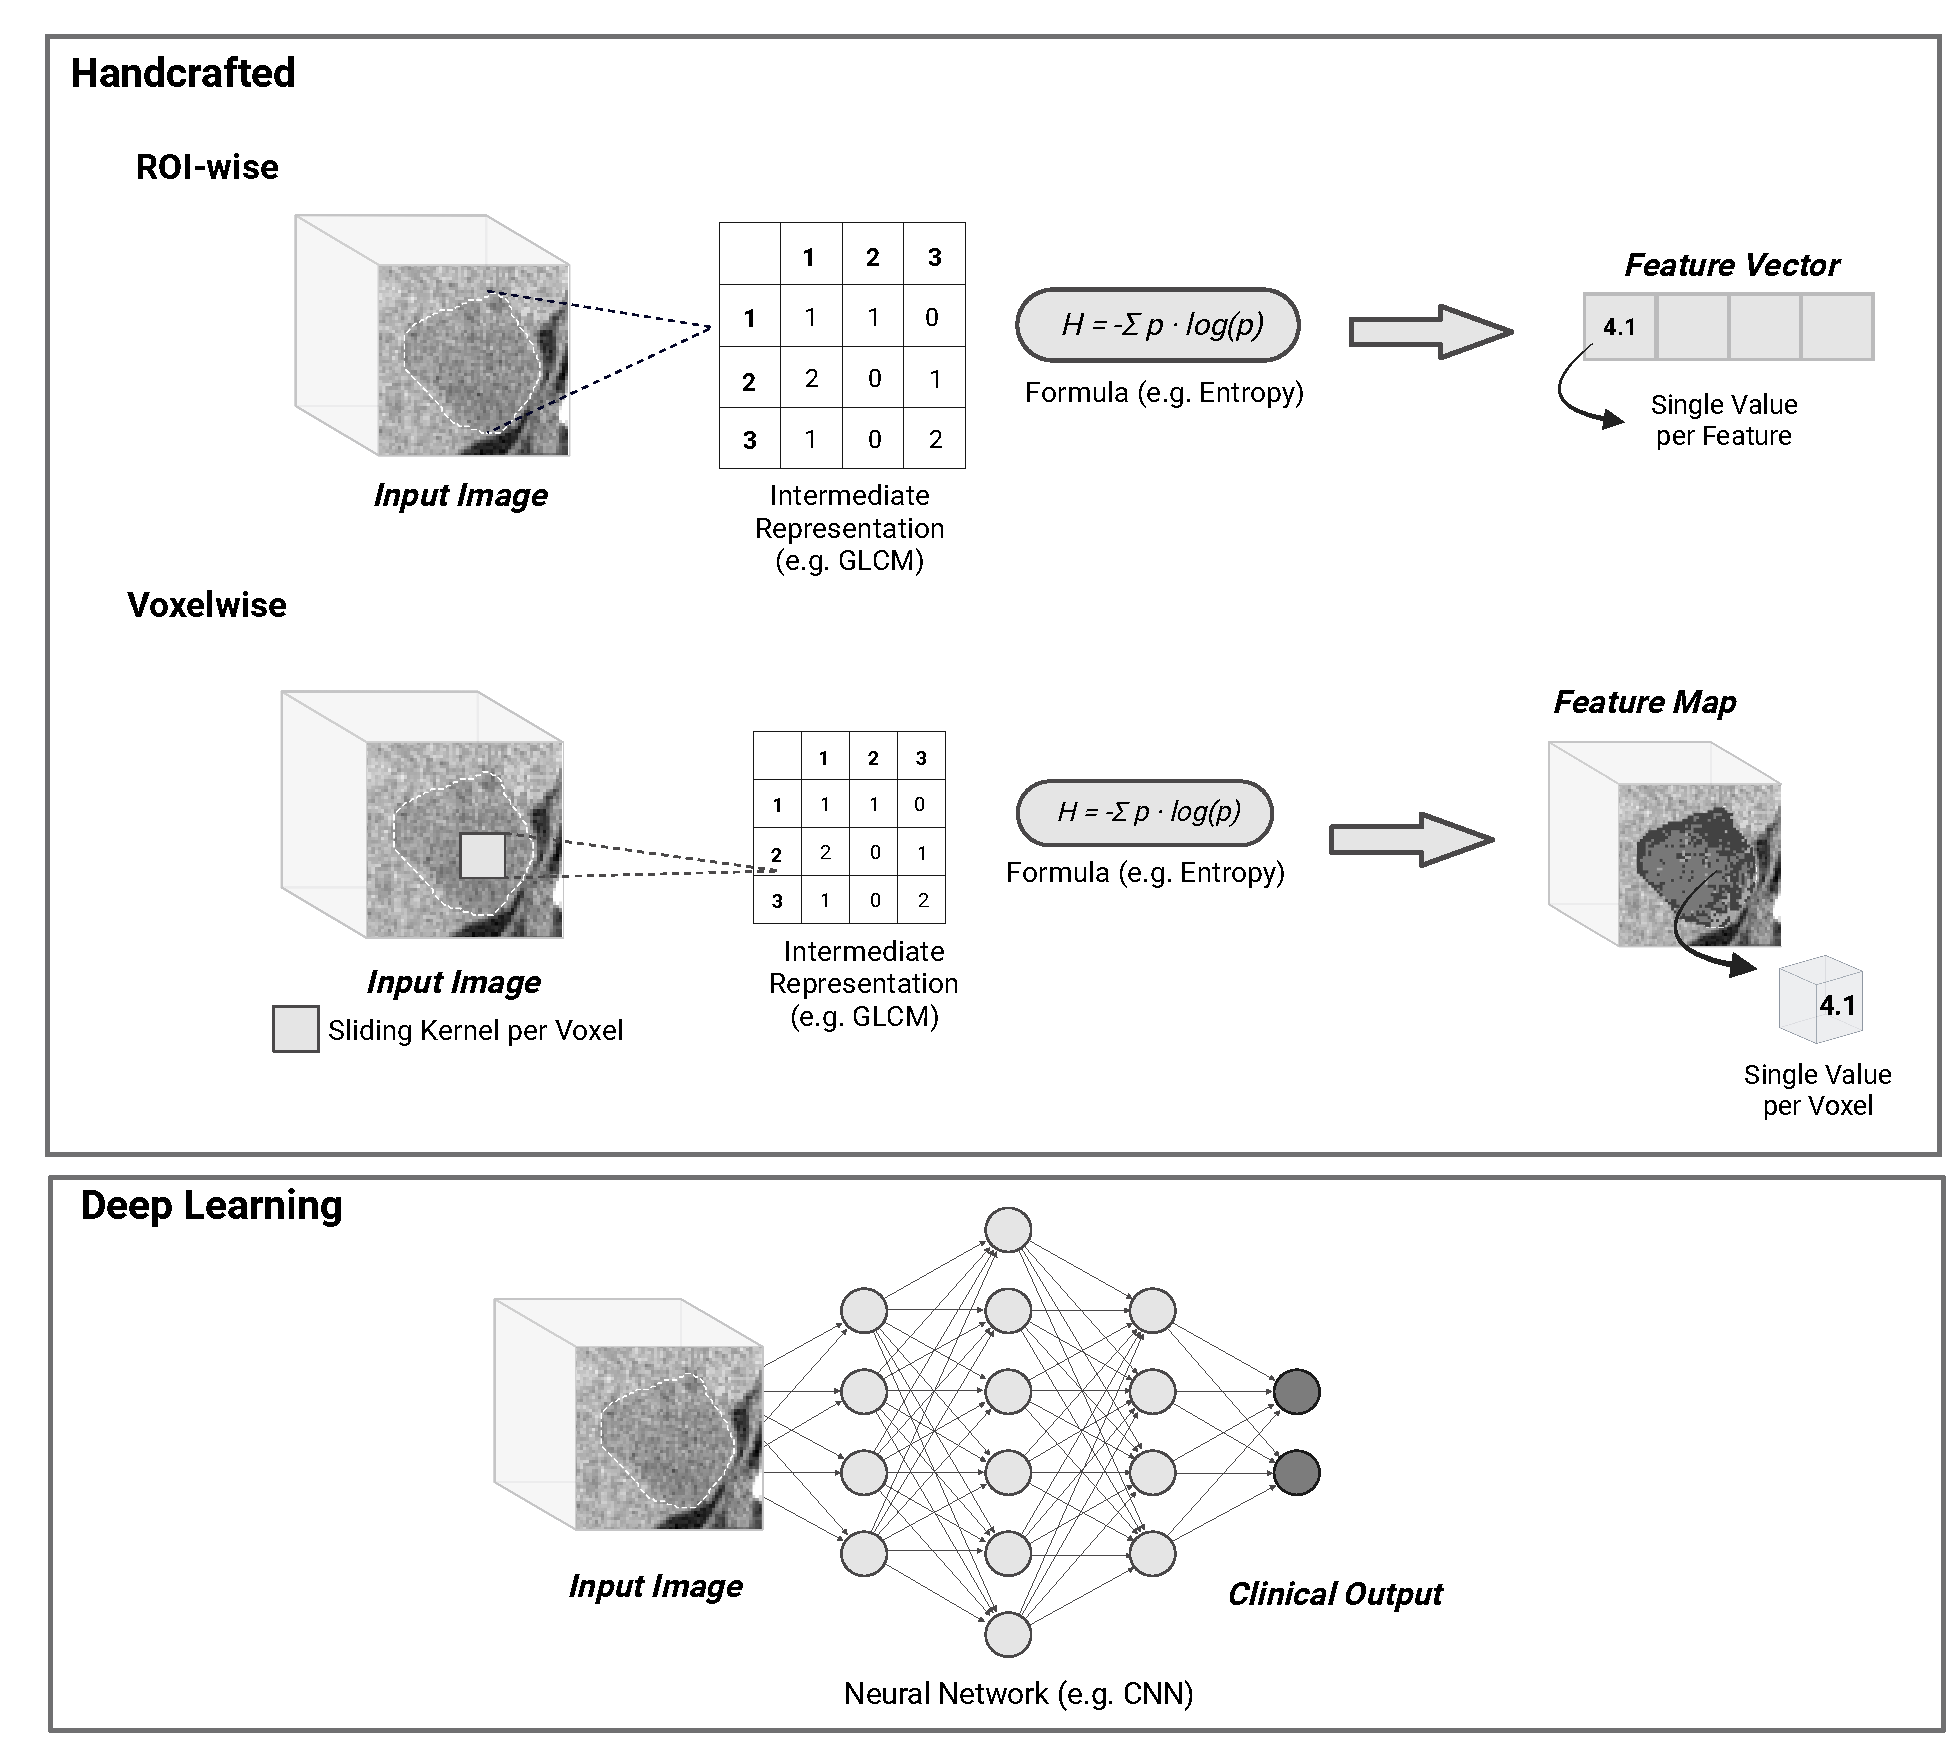
\includegraphics[width=0.95\textwidth]{fig_4_3.pdf}
\caption[Schematic comparison of radiomics feature extraction methods]{\textbf{Schematic comparison of radiomics feature extraction methods.}
Handcrafted Radiomics: Features are derived from explicit intermediate
mathematical representations, such as the Gray-Level Co-occurrence
Matrix (GLCM). In the ROI-wise approach (top), a single large GLCM is
accumulated over the entire tumor mask, and a formula (e.g., for
entropy) is applied once to yield a single global value. In the
Voxelwise approach (bottom), a small, local GLCM is computed within a
sliding kernel around each voxel. The formula is applied to this local
matrix, and the resulting value is assigned to the center voxel,
generating a spatial feature map. Deep Learning: The raw input image is
passed directly through a neural network (e.g., a CNN) to learn
abstract, hierarchical feature representations (embeddings) optimized
for a specific task, without explicit human-defined formulas or
intermediate matrix representations. Created with BioRender.com.}
\label{fig:4.3}
\end{figure}

The limitation of ROI-wise radiomics is that it implicitly assumes
tumors are sufficiently homogeneous that averaging captures their
essential properties. As discussed in Chapter~\ref{ch:3}, colorectal liver
metastases are histologically heterogeneous, with viable tumor,
necrosis, and fibrosis distributed in spatial patterns. Averaging over
this heterogeneity may discard clinically relevant information.



\section{Habitat Imaging}\label{habitat-imaging}

The idea of partitioning tumors into spatially distinct subregions based on imaging characteristics predates the term \emph{habitat}. In the 2000s and early 2010s, several studies already proposed the use of clustering algorithms to study intratumor heterogeneity (mainly necrosis and viable tumor) for several cancer types in preclinical models \citep{caranoQuantificationTumorTissue2004,divinePopulationBasedGaussianMixture2016,henningMultispectralQuantificationTissue2007} using PET and MRI imaging modalities.

The term habitat and its ecological framing were introduced in 2013
\citep{gatenbyQuantitativeImagingCancer2013}. Drawing on landscape ecology, they proposed that
tumors could be understood as ecosystems containing distinct habitats
with different environmental conditions. Just as a forest contains
distinct microenvironments with different species compositions, a tumor
contains regions with different blood flow, oxygenation, and cellular
populations. According to the authors, the heterogeneous environment may
drive tumor evolution (e.g., hypoxic habitats select for cells with
aggressive, therapy-resistant phenotypes) and therefore habitats might
be worth studying. This ecological framing was subsequently applied to
breast cancer DCE-MRI by the same group \citep{chaudhuryIdentifyingMetastaticBreast2015},
establishing the conceptual foundation for the field. The field remained
relatively small throughout the 2010s, with most radiomics research
focusing on supervised learning approaches that required whole-tumor
feature vectors.

To date, most habitat imaging studies have used MRI rather than CT.
This is mainly due to the richer biological information available from
multiparametric MRI: diffusion-weighted imaging provides the apparent
diffusion coefficient (ADC), which correlates with cellularity; dynamic
contrast-enhanced sequences yield perfusion parameters such as Ktrans
and ve; and T2-weighted imaging reflects tissue water content and edema.
These parameters have known relationships to tissue biology, making
habitat interpretation more straightforward.

This advantage was first demonstrated in glioblastoma, where Katiyar and
colleagues \citep{katiyarNovelUnsupervisedSegmentation2017} applied spatially regularised spectral
clustering to mpMRI in mouse xenografts, achieving strong
correlation with histological tissue fractions of necrosis and viable
tumor. This was later shown in breast cancer mouse models
\citep{jardim-perassiMultiparametricMRICoregistered2019}, where habitats derived from six MRI
parameters were validated against co-registered histology using
3D-printed tumor moulds (\Cref{fig:4.4}). The
resulting habitats corresponded to viable-normoxic, viable-hypoxic,
nonviable-hypoxic, and nonviable-normoxic tissue types, validated
against H\&E staining, pimonidazole (a hypoxia marker), and CD31 (a
vasculature marker). Beyond biological validation, imaging habitats have
been shown to correlate with clinical outcomes, mainly in glioblastoma
\citep{waqarVisualisingSpatialHeterogeneity2022}. The most prominent study computed vascular
habitats from perfusion MRI and demonstrated that they were highly
prognostic at presurgery \citep{juan-albarracinGlioblastomaVascularHabitats2018}.

\begin{figure}[htbp]
\centering
\includegraphics[width=0.95\textwidth]{fig_4_4.png}
\caption[Examples of MRI-based habitat imaging]{\textbf{Examples of MRI-based habitat imaging.}
\textbf{(A)} Preclinical breast cancer model illustrating biological
validation of imaging habitats. Habitats were defined by clustering six
MRI parameters (T2, T2*, ADC, and DCE kinetic metrics) using a Gaussian
Mixture Model. The resulting spatial maps (bottom center) were validated
against co-registered histology (right), where habitats correlated with
specific biological microenvironments: viable-normoxic (green),
viable-hypoxic (magenta/yellow), and nonviable/necrotic (blue) regions,
confirmed by H\&E, pimonidazole (hypoxia), and CD31 (vasculature)
staining. Adapted from Jardim-Perassi et al., 2019. \textbf{(B)}
Glioblastoma illustrating vascular habitats derived from perfusion MRI.
Tumors are partitioned into four distinct vascular habitats based on
perfusion characteristics: High Angiogenic Tumor (HAT, red), Low
Angiogenic Tumor (LAT, yellow), Infiltrated Peripheral Edema (IPE,
green), and Vasogenic Peripheral Edema (VPE, blue). These habitats have
been shown to differ in survival prognosis. Adapted from
Juan-Albarracín et al., 2018.}
\label{fig:4.4}
\end{figure}

CT-based habitat imaging has received less attention across all tumor
types, likely because CT provides fewer biologically interpretable
parameters. CECT reflects vascularity, and Hounsfield
units correlate broadly with tissue density, but the relationship
between CT intensity and specific tissue types is less direct than for
MRI-derived parameters.

Two studies have applied habitat imaging to colorectal liver metastases,
both using MRI rather than CT as well. In one study, researchers used
a semi-automated clustering approach based on PCA of DCE-MRI contrast
uptake curves to define regions of viable and non-viable tumor in 14
patients with CRLM scheduled for hepatic resection \citep{franklinTumourSubregionAnalysis2020}. Imaging-derived subregions showed good concordance with spatially
matched histology (mean Dice similarity coefficient 0.74 for viable
tumor), and pharmacokinetic parameters differed significantly between
viable and non-viable subregions. In \citep{katiyarQuantificationIntratumouralHeterogeneity2023} , the
authors applied a cross-species approach, training multi-view spectral
clustering on preclinical PET-MRI and applying it to six CRLM lesions
from four patients undergoing resection, with tissue fractions
correlating with histology. These studies provide proof-of-concept that
imaging habitats can reflect meaningful biological phenotypes in CRLM,
but sample sizes were small and the imaging modalities (DCE-MRI,
PET-MRI) are not routinely used for CRLM management.



Unlike supervised radiomics, where the pipeline is relatively
standardised (feature extraction, feature selection, model training),
there is no consensus pipeline for habitat imaging. Published studies
vary considerably in their methodological choices, and these differences
affect results in ways that are not fully understood
(\Cref{tab:habitat_studies}).

Studies differ in the features used for clustering: some use raw
intensity values from single or multiple imaging sequences, others use
derived parameters such as ADC or Ktrans, and still others compute
voxelwise texture features in local neighbourhoods before clustering.
K-means clustering dominates the literature due to its computational
efficiency and interpretability, though Gaussian mixture models offer
probabilistic assignments that may better reflect gradual transitions
between tissue types. The choice of cluster number (k) remains a central
challenge, with some studies fixing k a priori based on expected tissue
types and others using data-driven criteria such as the Calinski and
Harabasz score or the Bayesian Information Criterion \citep{schubertStopUsingElbow2023}.
Once habitats are defined, studies extract different metrics for
downstream analysis, ranging from simple volume fractions to texture
features within each habitat or spatial diversity indices. This
methodological heterogeneity makes comparison across studies difficult
and complicates efforts to establish habitat imaging as a reliable tool.

The lack of standardisation would be less problematic if habitat methods
were rigorously validated. However, validation remains the most
significant gap in the literature. The imaging biomarker roadmap for
cancer studies (O'Connor et al., 2017) describes three types of
validation: technical (is the measurement reproducible?), biological
(does it reflect true tissue properties?), and clinical (does it predict
outcomes independently of established factors?). Most habitat studies
fall short on all three criteria.

Technical validation, such as test-retest reproducibility or multi-site
stability, is reported in only a minority of studies. Biological
validation against histopathology requires resected specimens and
careful co-registration, which few studies achieve; most rely on
indirect evidence such as correlation with known physiology or gene
expression patterns. Clinical validation typically consists of survival
analysis, but external validation in independent cohorts is rare, and
few studies benchmark habitat metrics against tumor volume, a strong
prognostic factor that any new imaging biomarker should demonstrate
added value beyond.

Habitat imaging is virtually unexplored for colorectal liver metastases
despite strong biological rationale: the histopathological heterogeneity
of CRLM (viable tumor, necrosis, fibrosis) and its prognostic
significance suggest that spatial imaging phenotypes may carry clinical
information. The absence of CT-based habitat studies in CRLM, combined
with the broader validation gaps, motivated the work in this thesis. The
following chapters address these gaps through a staged approach: Chapter~\ref{ch:5} develops a standardised pipeline for CT-based habitat imaging in
CRLM, Chapter~\ref{ch:6} establishes technical precision through feature
stability analysis, Chapter~\ref{ch:7} provides biological validation using
multiparametric MRI as a reference, and Chapter~\ref{ch:8} assesses clinical
utility by benchmarking habitat metrics against volume across treatment
contexts.

\begin{table}[ht]
    \centering
    \small
    \caption[Summary of selected habitat imaging studies]{\textbf{Summary of selected habitat imaging studies.} Studies are listed chronologically. Technical validation refers to test-retest reproducibility or multi-site stability; biological validation refers to correlation with histopathology or known tissue biology; clinical validation refers to outcome prediction. GBM: glioblastoma; GMM: Gaussian mixture model.}
    \label{tab:habitat_studies}
    
    \begin{tabularx}{\textwidth}{@{} l >{\centering\arraybackslash}X >{\centering\arraybackslash}X >{\centering\arraybackslash}X c >{\centering\arraybackslash}X >{\centering\arraybackslash}X >{\centering\arraybackslash}X @{}}
        \toprule
        \textbf{Study} & \textbf{\makecell{Cancer\\type}} & \textbf{Modality} & \textbf{Method} & \textbf{\textit{k}} & \textbf{\makecell{Tech.\\Val.}} & \textbf{\makecell{Biol.\\Val.}} & \textbf{\makecell{Clin.\\Val.}} \\
        \midrule
        \citep{caranoQuantificationTumorTissue2004} & \makecell{Colorectal\\(preclinical)} & MRI & K-means & 4 & No & \makecell{Yes\\(histo.)} & No \\ \addlinespace
        \citep{henningMultispectralQuantificationTissue2007} & \makecell{Sarcoma\\(preclinical)} & MRI & K-means & 4 & No & \makecell{Yes\\(histo.)} & No \\ \addlinespace
        \citep{chaudhuryIdentifyingMetastaticBreast2015} & Breast & MRI & K-means & 4 & No & No & \makecell{Yes\\(molecular)} \\ \addlinespace
        \citep{divinePopulationBasedGaussianMixture2016} & \makecell{Breast\\(preclinical)} & \makecell{PET/\\MRI} & GMM & 5 & No & \makecell{Yes\\(histo.)} & No \\ \addlinespace
        \citep{katiyarNovelUnsupervisedSegmentation2017} & \makecell{GBM\\(preclinical)} & MRI & Spectral & 3 & No & \makecell{Yes\\(histo.)} & No \\ \addlinespace
        \citep{juan-albarracinGlioblastomaVascularHabitats2018} & GBM & MRI & K-means & 4 & No & \makecell{Yes\\(vascular)} & \makecell{Yes\\(survival)} \\ \addlinespace
        \citep{jardim-perassiMultiparametricMRICoregistered2019} & \makecell{Breast\\(preclinical)} & MRI & GMM & 4 & \makecell{Yes\\(repeat.)} & \makecell{Yes\\(histo.)} & No \\ \addlinespace
        \citep{franklinTumourSubregionAnalysis2020} & CRLM & MRI & K-means & 2 & No & \makecell{Yes\\(histo.)} & No \\ \addlinespace
        \citep{katiyarQuantificationIntratumouralHeterogeneity2023} & CRLM & \makecell{PET/\\MRI} & Spectral & 2 & No & \makecell{Yes\\(histo.)} & No \\
        \bottomrule
    \end{tabularx}
\end{table}


  
  \part{Methodological Framework}
  \vfill
  \begin{flushright}
  \begin{minipage}{0.75\textwidth}
  \raggedleft
  \large\itshape
  ``Science is a bit like the joke about the drunk who is looking under a
  lamppost for a key that he has lost on the other side of the street,
  because that's where the light is. It has no other choice.''
  
  \vspace{0.5cm}
  \upshape\normalsize --- Noam Chomsky
  \end{minipage}
  \end{flushright}
  \vfill
  \cleardoublepage
  \chapter{Data and Habitat Imaging
Pipeline}\label{data-and-habitat-imaging-pipeline}\label{ch:5}

This chapter describes the datasets and methods that support the
experiments carried out in this thesis. We begin by introducing the four
main patient cohorts and their role in habitat model development,
validation, and clinical application (Section 5.1). We then present the
habitat imaging pipeline (Section 5.2), our end-to-end framework for
computing tumor habitats from medical images.

\section{Patient Cohorts}\label{patient-cohorts}

\begin{figure}[htbp]
\centering
\includegraphics[width=0.95\textwidth]{fig_5_1.pdf}
\caption[Overview of patient cohorts used in this thesis]{\textbf{Overview of patient cohorts used in this thesis.}
Prospective cohorts provide multiparametric imaging (PREDICT) and
histology (POEM) for developing and validating the biologically-informed
habitat model. Retrospective cohorts (blue) provide large-scale CT
imaging with clinical outcomes for applying the habitat model and
assessing its clinical relevance. Numbers indicate patients and tumors
remaining after exclusions.}
\label{fig:5.1}
\end{figure}

This thesis is based on four main datasets of colorectal cancer patients
with liver metastases, each serving a distinct role in the development,
validation, and clinical application of CT-derived tumor habitats
(\Cref{tab:datasets}, \Cref{fig:5.1}). For the development and
biological validation of the habitat model we used two small prospective
cohorts: PREDICT (n=10 patients, 42 tumors) provides co-registered
multiparametric MRI (mpMRI) to anchor CT-derived habitats to
quantitative imaging proxies of vascularity and cellularity, while POEM
(n=6 patients, 6 tumors) provides whole-tumor histopathology for
independent validation. Two large retrospective cohorts---TCIA (n=189
patients, 389 tumors) and VHIO (n=343 patients, 1759 tumors)---provide
portal-phase CT imaging alongside clinical outcomes and are used to
apply the biologically-informed habitat model (developed in Chapter~\ref{ch:7})
and assess its prognostic value (Chapter~\ref{ch:8}). Detailed demographic and
clinical characteristics of TCIA and VHIO are provided in Chapter~\ref{ch:8}.

Chapter~\ref{ch:6} presents a broader technical study assessing the precision of
3D voxelwise radiomics features using additional retrospective data from
both liver and lung lesions. That analysis established which handcrafted
features are sufficiently robust for habitat computation and informed
the feature selection strategy used in Chapter 7. The datasets described
here---PREDICT, POEM, TCIA, and VHIO---form the foundation for the
biologically-informed habitat model and its clinical translation, which
are the central contributions of this thesis.

\begin{table}[ht]
    \centering
    \small
    \caption[Summary of datasets and their role in this thesis]{\textbf{Summary of datasets and their role in this thesis.} PREDICT provides co-registered mpMRI for biologically-informed habitat model development; POEM provides histology for independent validation. TCIA and VHIO provide large-scale CT imaging with survival outcomes for applying the habitat model and testing its prognostic value. OS: overall survival; PFS: progression-free survival; DFS: disease-free survival; mpMRI: multiparametric MRI; HE: hematoxylin and eosin.}
    \label{tab:datasets}
    
    \begin{tabularx}{\textwidth}{@{} l c c >{\raggedright\arraybackslash}X c >{\raggedright\arraybackslash}X @{}}
        \toprule
        \textbf{Dataset} & \textbf{\makecell{N\\patients}} & \textbf{\makecell{N\\tumors}} & \textbf{Imaging modalities} & \textbf{\makecell{Clinical\\outcome}} & \textbf{Primary use} \\
        \midrule
        PREDICT & 10 & 42 & CT (Portal Phase), MRI & --- & Habitat model development (mpMRI-anchored) and validation (Chapter~\ref{ch:7}) \\ \addlinespace
        POEM & 6 & 6 & CT (Portal Phase), Histology (HE) & --- & Biological validation of habitat model (Chapter~\ref{ch:7}) \\ \addlinespace
        TCIA & 189 & 389 & CT (Portal Phase) & OS, DFS & Application of habitat model and clinical outcome modeling (Chapter~\ref{ch:8}) \\ \addlinespace
        VHIO & 343 & 1759 & CT (Portal Phase) & OS, PFS & Application of habitat model and clinical outcome modeling (Chapter~\ref{ch:8}) \\
        \bottomrule
    \end{tabularx}
\end{table}

All cohorts were collected as part of ongoing studies approved by the
Vall d'Hebron University Hospital Ethics Committee: PR(AG)29/2020
(PREDICT), PR(AG)305/2024 (POEM), PR(AG)335/2018 and PR(AG)500/2023
(VHIO). Patients provided written informed consent to participate in
such studies.

\subsection{CT Image Preprocessing}\label{ct-image-preprocessing}

All CT images were acquired in the portal venous phase with
intravenous contrast, tube voltage of 100-130kV, slice thickness of
1.25-5mm and pixel size 0.7-1.1mm\textsuperscript{2}, and stored in
DICOM format (\emph{Digital Imaging and Communications in Medicine
(DICOM) Standard} \citep{DigitalImagingCommunications2025}). PREDICT and VHIO scans were retrieved from the
Vall d\textquotesingle Hebron Hospital imaging archive (Picture
Archiving and Communication System, PACS), anonymized with an
identifiable patient ID, and transferred to a password-protected VHIO
storage server. TCIA scans were downloaded from the public repository
(\url{https://www.cancerimagingarchive.net/}). POEM scans were provided
through a collaborative project with Hospital Universitari de Bellvitge
(see Section 5.1.3.) DICOM files were converted to NIfTI (Neuroimaging
Informatics Technology Initiative) format using dcm2niix \citep{liFirstStepNeuroimaging2016},

Images underwent qualitative assessment by both the author and the
group's experienced radiologists to ensure acquisition quality and
suitability for analysis. Scans were excluded if they were
non-contrast-enhanced, acquired outside the portal venous phase, did not
include the entire liver, or showed no measurable disease at baseline
(defined as liver lesions \textless1 cm in diameter or absent liver
metastases). \Cref{fig:5.1} summarizes exclusion counts for
each cohort.

For the majority of the scans, tumor segmentation was performed manually
using 3D Slicer \citep{fedorov3DSlicerImage2012}. For PREDICT and POEM, all
well-defined target lesions per patient were delineated by the group's
experienced radiologists. For VHIO cohort, a third of the tumors
(\textasciitilde600) were manually delineated by the author and
supervised by an experienced radiologist. The rest were automatically
delineated by SALSA, an automated liver tumor segmentation tool
developed in our lab during the course of this thesis, with manual
correction when needed. For TCIA, manual segmentations were performed by
radiologists as part of the original data collection \citep{simpsonPreoperativeCTSurvival2024}

Voxel resampling and intensity preprocessing were performed during
feature extraction (see Methods Section of Chapters 6 and 7), ensuring
consistent spatial resolution and intensity normalization across all
voxelwise feature maps.

\subsection{Multiparametric MRI Preprocessing (PREDICT)}\label{multiparametric-mri-preprocessing-predict}

The PREDICT cohort included contrast-enhanced CT alongside
mpMRI acquired on two scanners: a 1.5T Siemens
Avanto and a 3T GE SIGNA Pioneer. The MRI protocol included
high-resolution anatomical imaging (T2-weighted and T1-weighted),
advanced diffusion MRI with multiple b-values and echo times, variable
flip angle spoiled gradient echo (SGrE) imaging for T1 mapping, and
dynamic contrast-enhanced (DCE) MRI. Full acquisition parameters are
provided in Annex A.

MRI preprocessing was performed by MRI physicist F. Grussu, and included
denoising (MP-PCA) \citep{veraartDenoisingDiffusionMRI2016}, Gibbs unringing \citep{kellnerGibbsringingArtifactRemoval2016}, motion correction via affine coregistration \citep{ourselinReconstructing3DStructure2001}, and EPI distortion correction using reversed phase-encoding
acquisitions \citep{anderssonHowCorrectSusceptibility2003}. Anatomical images underwent N4
bias field correction based on ANTs \citep{avantsSymmetricDiffeomorphicImage2008}. Tumor
segmentations were drawn manually by an experienced radiologist on the
T2-weighted scan, aided by visual inspection of all MRI contrasts.

From the preprocessed MRI data, thirteen multiparametric (mpMRI) maps
were derived using biophysical models (\Cref{tab:mpmri_maps}). Diffusion-relaxation MRI was modeled using two approaches: (1) a
two-pool system capturing tissue and vascular water contributions,
yielding apparent diffusion coefficients ($ADC_t$, $ADC_v$), corresponding to
tissue and vascular water contributions, transverse relaxation times
($T_{2t}$), vascular signal fraction ($f_v$), and tissue kurtosis excess ($K_t$);
and (2) an advanced microstructural model \citep{grussuClinicallyFeasibleLiver2025}
incorporating intra- and extracellular compartments, yielding intrinsic
diffusivity ($D_0$), volume-weighted cell size ($vCS$), intracellular
fraction ($f_{in}$), and cell density. Variable flip angle imaging provided
total longitudinal relaxation time ($T_1$). DCE MRI was fitted using a
two-compartment Tofts model \citep{toftsModelingTracerKinetics1997}, yielding the capillary
permeability constant ($K^{trans}$), plasma volume fraction
($v_p$), and extracellular-extravascular volume fraction ($v_e$). Model
fitting was performed using custom Python code available at
\url{https://github.com/fragrussu/MyRelax} and
\url{https://github.com/fragrussu/bodymritools}.

\begin{table}[ht]
    \centering
    \small
    \caption[Multiparametric MRI maps used for CT habitat development]{\textbf{Multiparametric MRI maps used for CT habitat development.} Thirteen quantitative maps were derived from diffusion-relaxation MRI, variable flip angle T1 mapping, and dynamic contrast-enhanced MRI.}
    \label{tab:mpmri_maps}
    
    \begin{tabularx}{\textwidth}{@{} l l l c >{\raggedright\arraybackslash}X @{}}
        \toprule
        \multicolumn{2}{c}{\textbf{mpMRI metric}} & \textbf{Computed from} & \textbf{Units} & \textbf{Description} \\
        \cmidrule(r){1-2}
        $ADC_t$ & Tissue ADC & Diffusion-relaxation MRI & $\mu m^2/ms$ & Apparent diffusivity of water in tissue (excluding vasculature) \\ \addlinespace
        $ADC_v$ & Vascular ADC & Diffusion-relaxation MRI & $\mu m^2/ms$ & Apparent diffusivity in vascular compartment (IVIM effect) \\ \addlinespace
        $K_t$ & Tissue kurtosis excess & Diffusion-relaxation MRI & Dim.less & Quantifies non-Gaussian diffusion due to heterogeneity or restriction \\ \addlinespace
        $f_v$ & Vascular signal fraction & Diffusion-relaxation MRI & Norm. & Signal arising from vascular compartment (IVIM) \\ \addlinespace
        $T_{2t}$ & Tissue $T_2$ & Diffusion-relaxation MRI & ms & Transverse relaxation time of tissue (excluding vasculature) \\ \addlinespace
        $D_0$ & Intrinsic diffusivity & Advanced diffusion model & $\mu m^2/ms$ & Intrinsic intracellular diffusivity \\ \addlinespace
        $vCS$ & Vol-weighted cell size & Advanced diffusion model & $\mu m$ & Average cell size weighted by cell volume \\ \addlinespace
        $f_{in}$ & Intracellular fraction & Advanced diffusion model & Norm. & Fraction of signal arising from intracellular water \\ \addlinespace
        $CD$ & Cell density & Advanced diffusion model & Cells/$mm^3$ & Estimated cell density (derived from $f_{in}$ and $vCS$) \\ \addlinespace
        $T_1$ & $T_1$ & Variable flip angle SGrE & ms & Total longitudinal relaxation time \\ \addlinespace
        $T_2^*$ & $T_2^*$ & Multiecho SGrE & ms & Effective transverse relaxation time \\ \addlinespace
        $K^{trans}$ & Capillary permeability & DCE MRI & $min^{-1}$ & Influx mass transfer rate of contrast agent \\ \addlinespace
        $v_e$ & EES volume & DCE MRI & Norm. & Volume of extracellular, extravascular space per unit tissue volume \\
        \bottomrule
    \end{tabularx}
\end{table}

We harmonized mpMRI metrics across scanners with a custom-written ComBat
\citep{fortinHarmonizationCorticalThickness2018} implementation, rescaling metrics obtained on the
1.5T system to the 3T range. Quality control ensured that all mpMRI
values were biologically plausible. For each metric, we established a
valid range based on empirical knowledge (Annex A). Voxels within this
range were included, those marginally outside (±10\%) were clipped to
the boundary, and those beyond this tolerance were excluded.



\subsection{Histopathology Workflow (POEM)}\label{histopathology-workflow-poem}

The POEM cohort (PrOspEctive Metastases Imaging) was collected as part
of a multicenter observational study led by Dr. Peter Vermeulen (GZA
Hospitals, Belgium) in collaboration with Hospital Universitari de
Bellvitge (Spain). The study aims to develop radiomic signatures of
histopathological growth patterns \citep{lataczCanMedicalImaging2021} in liver
metastases from colorectal and breast cancer using standard-of-care CT
and MRI alongside complete histopathological sampling \citep{lataczProspectiveCompleteHistopathological2024}. Our analysis focused on colorectal liver metastases from patients
treated at Hospital Universitari de Bellvitge who underwent complete
tumor resection.

The histopathology protocol was designed to preserve spatial orientation
for comparison with preoperative imaging. Surgeons applied orientation
marks to the resected specimen, allowing the pathologist to slice the
tissue in transverse (axial) planes corresponding to CT and MRI
imaging planes. Slices were cut at 0.5--1 cm thickness, photographed,
and sampled systematically. Tissue samples were formalin-fixed,
paraffin-embedded, and stained with hematoxylin and eosin (H\&E).
Whole-slide images were acquired using a 3DHISTECH Pannoramic-series
scanner, producing MRXS files.

Histological annotations of necrosis, viable cancer and fibrosis/stroma
were automatically performed using QuPath \citep{bankheadQuPathOpenSource2017}, an
open-source digital pathology platform, and supervised by an experienced
pathologist. An experienced pathologist manually delineated regions of
necrosis, fibrosis, and viable tumor on digitized whole-slide images.
These annotations provided qualitative ground truth for validating
CT-derived habitats (Chapter~\ref{ch:7}). We attempted spatial coregistration
between histology slices and corresponding CT slices but found it
impractical due to tissue deformation during resection and processing.
As a result, histology was used for qualitative biological validation
rather than voxel-by-voxel spatial comparison.

\section{Habitat Imaging Pipeline}\label{habitat-imaging-pipeline}

Habitat imaging is becoming increasingly popular in oncology as a way to
segment tumors into meaningful radiological subregions. Yet despite a
growing literature, there is no standard tool for computing habitats.
Each study implements its own custom-built codes, which are rarely
shared and in the case they are, poorly documented. Any researcher
interested in habitat imaging faces the same challenges repeatedly: how
to preprocess voxelwise features, how to choose the clustering
algorithm, how to ensure habitat labels are across patients are
consistent so that ``Habitat 1'' means the same thing in every case,
etc.

These are not trivial implementation choices. A pipeline that ignores
voxel spacing differences will produce habitats that reflect acquistion
parameters rather than biology. A pipeline that clusters all tumors
together may dilute tumor-specific heterogeneity into noise. The
experiments carried out in Chapter~\ref{ch:6} made these challenges concrete for
us. Computing habitats for the precision analysis requires solvign each
of these problems from scratch, and the solutions were tied to the
specific dataset and analysis.

To enable the work in Chapters 7 and 8, and to support future research,
we developed a modular, documented pipeline that addresses these issues
systematically. The pipeline is image-modality agnostic, being
applicable to any voxelwise imaging data (CT, MRI, PET, etc.) and
works with both 2D and 3D data. It also includes key design choices as
configurable parameters rather than hardcoded assumptions. We are
currently preparing the pipeline for public release as an open-source
tool, available at
https://github.com/radiomicsgroup/imaging-habitats-pipeline. We share it
with the hope that it saves other researchers the substantial time and
effort required to build habitat imaging workflows from scratch, and
that it helps standardize methods across studies to improve
reproducibility and comparability in the field.

\subsection{Pipeline Overview}\label{pipeline-overview}

The pipeline consists of three modules: Preprocessing, Clustering, and
Analysis (\Cref{fig:5.2}):

\begin{itemize}
\item
  \textbf{Preprocessing} takes voxelwise feature maps (e.g., Kurtosis,
  ADC, Coarseness) as 3D NIfTI files, removes background voxels,
  enforces consistent array shapes across maps, and applies feature
  scaling. The output is a 4D NIfTI volume per tumor (dimensions: x, y,
  z, features), with both scaled and unscaled versions preserved for
  transparency. Background voxels are automatically detected and masked
  out, and all feature maps are checked for spatial alignment.
\item
  \textbf{Clustering} takes the preprocessed 4D volumes and assigns each
  voxel to a habitat. The module supports multiple algorithms (Gaussian
  Mixture Models, K-means, Bayesian GMM, HDBSCAN) and allows the number
  of clusters to be set manually or selected via data-driven criteria
  (BIC, silhouette score). Cluster labels are integers starting at 1;
  background is reserved as 0.
\item
  \textbf{Analysis} computes habitat-derived metrics (described in
  Section 5.2.4) and exports summary statistics as CSV files for
  downstream analysis.
\end{itemize}

\begin{figure}[t!]
\centering
\includegraphics[width=0.95\textwidth]{fig_5_2.pdf}
\caption[Habitat imaging pipeline overview]{\textbf{Habitat imaging pipeline overview.}
The pipeline consists of three modules. Preprocessing removes background
voxels, applies optional log transformation, and performs standard
scaling, outputting a 4D NIfTI volume per tumor. Clustering assigns
voxels to habitats using GMM, K-means, Bayesian GMM, or HDBSCAN, with
automatic or manual selection of cluster number. Three clustering scopes
are available: single-tumor, pooled, or hybrid (Figure~\ref{fig:5.3}). Analysis computes
habitat-derived metrics (proportions, entropy, rim/core statistics) and
exports summary tables.}
\label{fig:5.2}
\end{figure}



The pipeline is implemented in Python and can be run from the command
line. All random seeds are exposed for reproducibility, and outputs are
organized by experiment name to support version control.

\subsection{Key Implementation Choices}\label{key-implementation-choices}

\textbf{Voxel resampling.} Texture features describe spatial
relationships between neighboring voxels, which means their values
depend on voxel dimensions. A feature computed on a 0.7×0.7×1.0 mm grid
is not directly comparable to the same feature computed on a 0.9×0.9×2.5
mm grid. For cross-tumor comparisons to be meaningful, input images
should be resampled to a common isotropic resolution before feature
extraction. The pipeline itself does not yet perform resampling---it
expects preprocessed inputs---but users working with heterogeneous
acquisitions should resample upstream since results may reflect
acquisition differences rather than biology.

\textbf{Feature scaling.} Clustering algorithms are sensitive to feature
magnitudes. If one feature ranges from 0 to 1 and another from 0 to
10,000, the latter will dominate distance calculations regardless of its
biological relevance. We apply standard scaling (zero mean, unit
variance) to all features before clustering. The scaler can be fit per
tumor, per patient, or across the full cohort, depending on the analysis
goal. For the studies in this thesis, we fit a single scaler across all
voxels being processed, ensuring that habitat definitions are comparable
across tumors.

\textbf{Log transformation.} Some imaging metrics span several orders of
magnitude and exhibit strong right skew---ADC values, T1 relaxation
times, and permeability coefficients are common examples. Clustering
such features in their raw form can produce habitats driven by outliers
rather than typical tissue properties. We assess each
feature\textquotesingle s distribution (skewness, dynamic range,
coefficient of variation) and apply log transformation where
appropriate, excluding bounded fractions (e.g., volume fractions
constrained to {[}0,1{]}) to preserve their probabilistic
interpretation. This is not a universal preprocessing step; it is a
decision that must be made feature by feature, with the goal of
presenting the clustering algorithm with distributions that reflect
meaningful biological variation rather than measurement artifacts.

\textbf{Clustering algorithm and number of clusters.} The pipeline
supports multiple clustering algorithms: Gaussian Mixture Models (GMM),
K-means, and HDBSCAN. GMM is our default because it provides
probabilistic (soft) assignments that better capture gradual transitions
between tumor phenotypes---biologically plausible given partial volume
effects and mixed tissue interfaces. However, users may prefer hard
assignments or density-based clustering depending on their application.
The number of clusters can be specified manually or determined
automatically using different criteria such as the Bayesian Information
Criterion (BIC) or the Silhouette Score.

\textbf{Clustering Scope:} A critical design choice is whether to
cluster each tumor individually or pool all tumors together. The
pipeline supports three modes (\Cref{fig:5.3}):

\begin{figure}[t!]
\centering
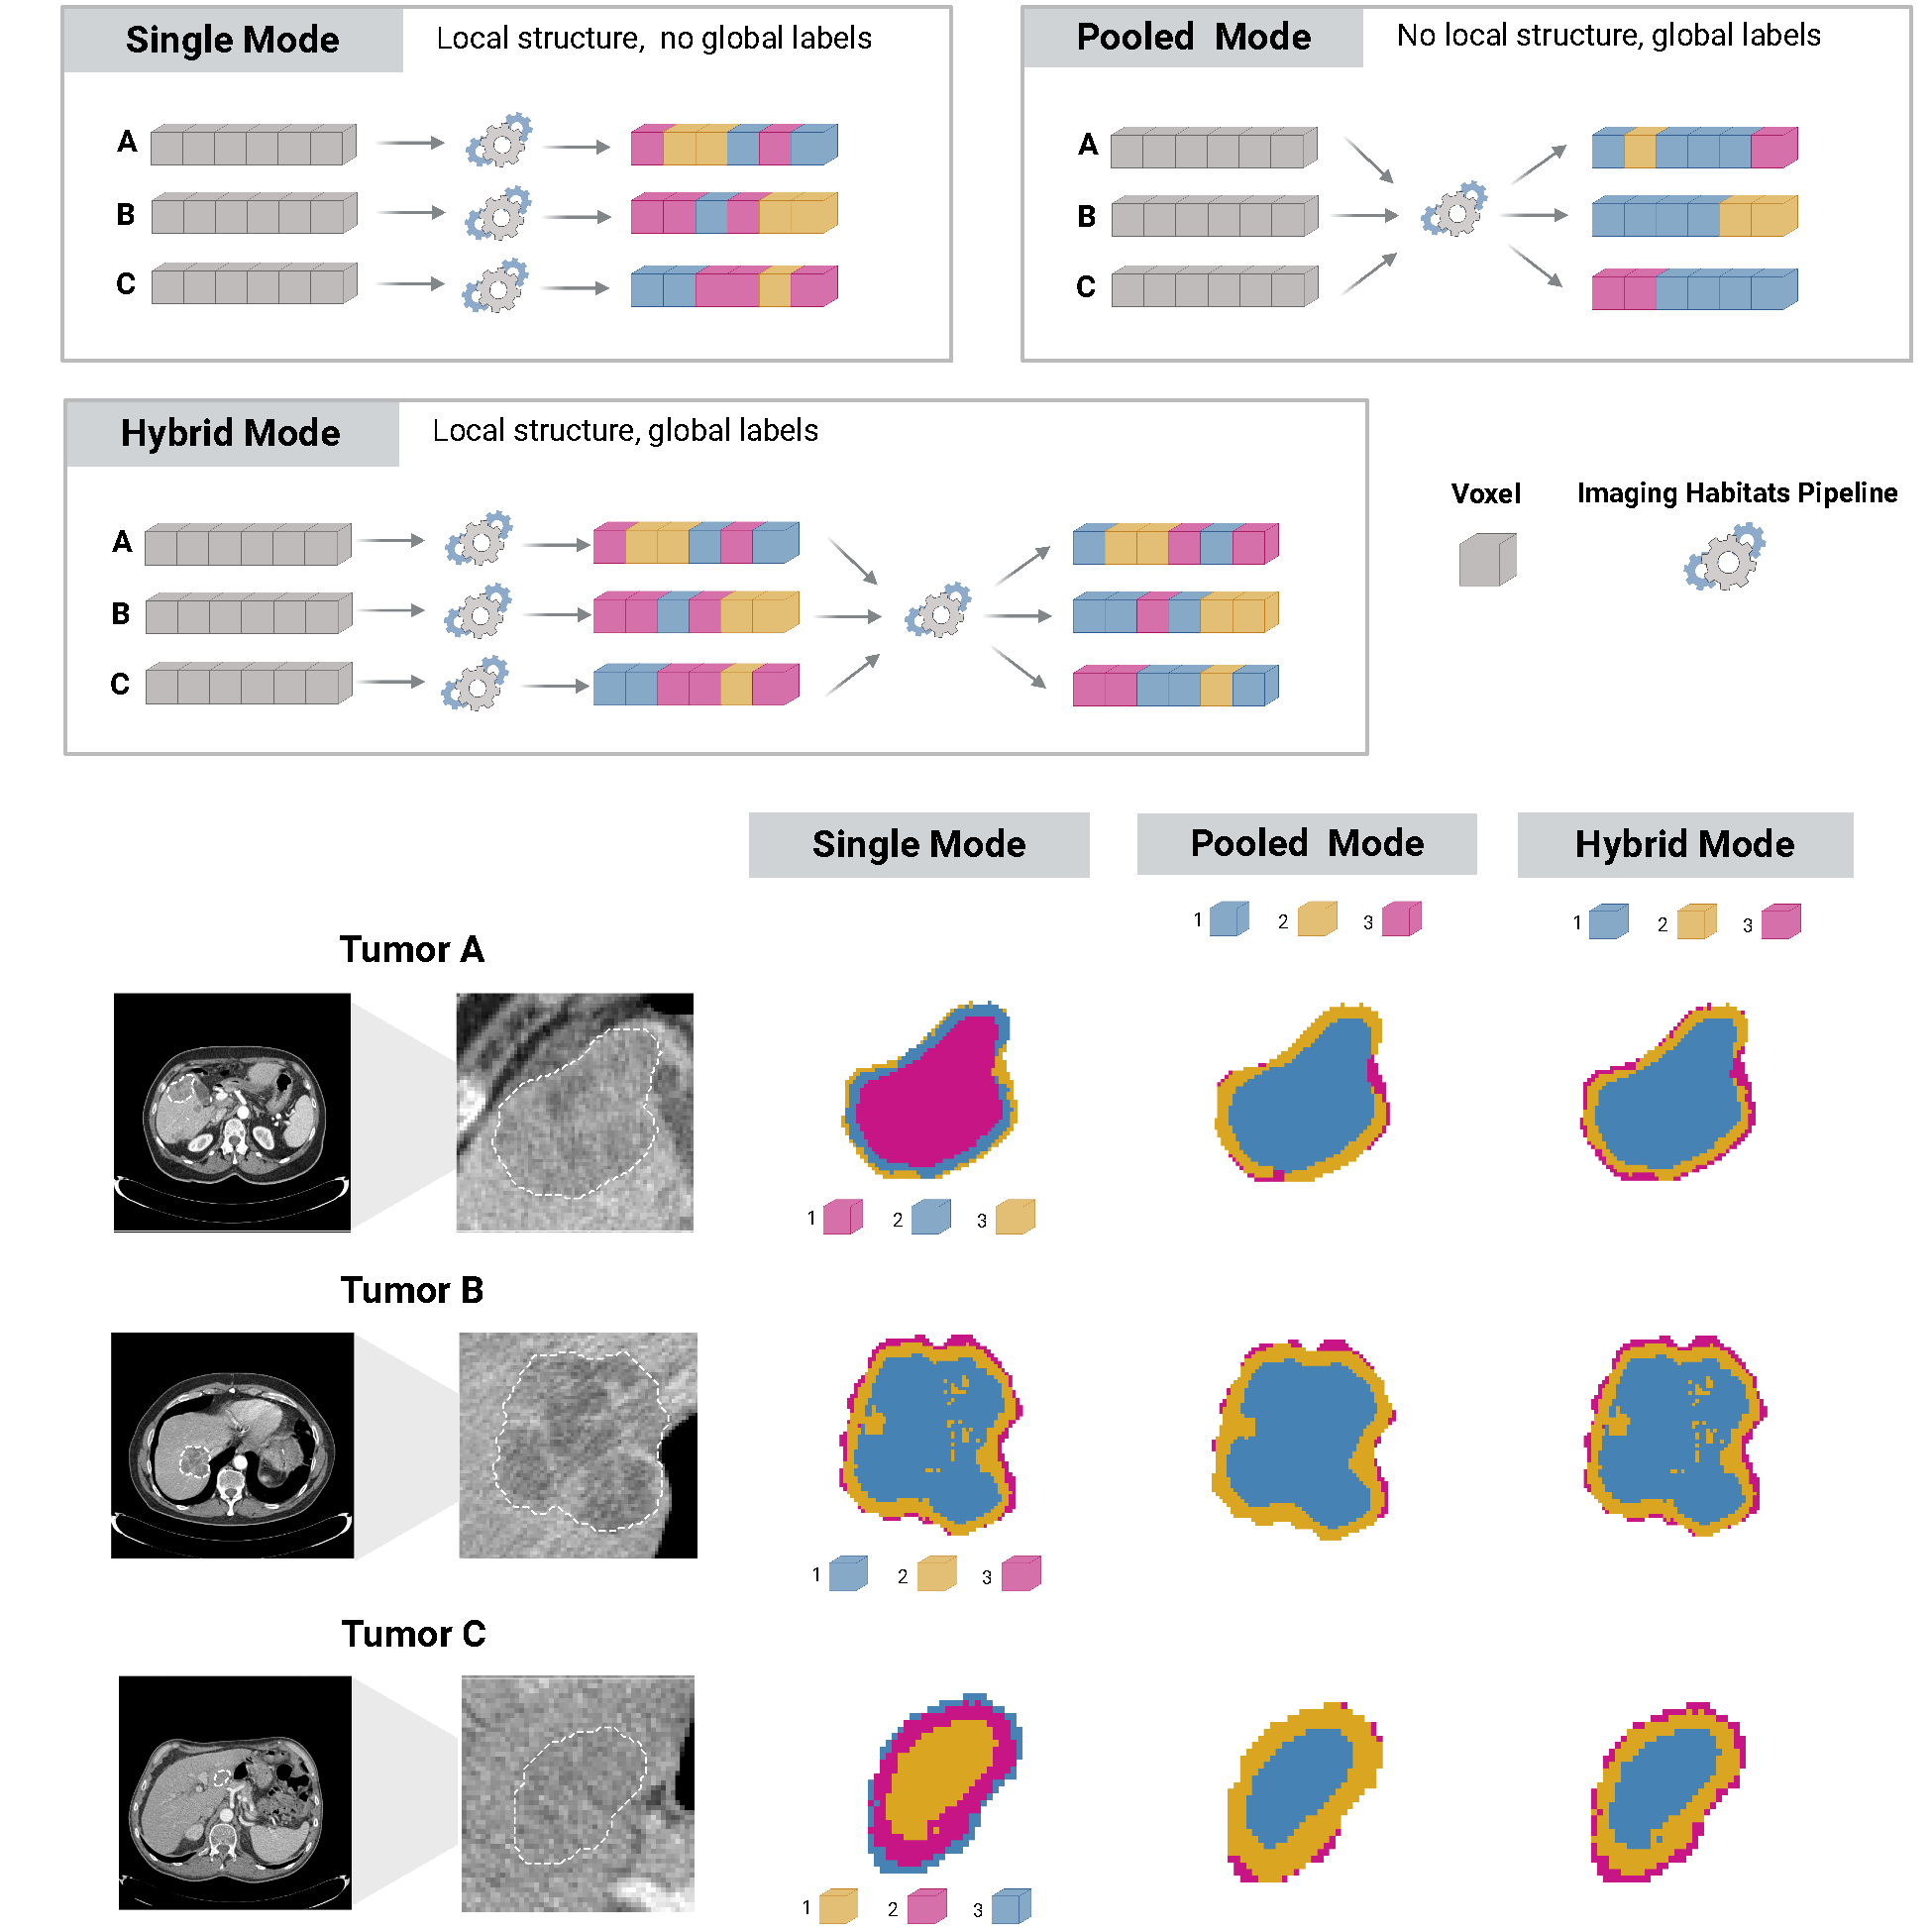
\includegraphics[width=0.9\textwidth]{fig_5_3.pdf}
\caption[Clustering scope: single-tumor, pooled, and hybrid modes]{\textbf{Clustering scope: single-tumor, pooled, and hybrid modes.}
\textbf{(A)} Single-tumor mode. Each tumor is clustered independently.
Labels are arbitrary and not comparable across tumors. \textbf{(B)}
Pooled mode. All voxels are clustered together, producing globally
consistent labels. However, local heterogeneity may be diluted.
\textbf{(C)} Hybrid mode. Tumors are first clustered locally, then local
cluster centroids are pooled and meta-clustered to define global
prototypes. Each local cluster is mapped to its nearest prototype,
yielding consistent labels while preserving local structure.}
\label{fig:5.3}
\end{figure}

\emph{Single-tumor mode} clusters each tumor independently. This
preserves local heterogeneity patterns but produces arbitrary label
IDs---"Cluster 1" in Tumor A might represent necrosis, while "Cluster 1"
in Tumor B might represent highly perfused tissue. Cross-patient
comparisons require post-hoc label alignment.

\emph{Pooled mode} stacks all voxels from all tumors and clusters them
in a single run. Labels are globally consistent by construction: every
voxel in the cohort is assigned to one of K shared habitats. However,
pooling can dilute tumor-specific patterns. If one tumor is
predominantly necrotic and another highly vascular, the algorithm may
find "average" habitats that represent neither tumor well. Inter-tumor
variability in baseline intensities can dominate the clustering,
obscuring biologically meaningful intra-tumor structure.

\emph{Hybrid mode} combines both strategies through a two-level
approach:

\begin{enumerate}
\def\labelenumi{\arabic{enumi}.}
\item
  \emph{Local clustering}: Each tumor is clustered independently (as in
  single-tumor mode), preserving fine-grained heterogeneity.
\item
  \emph{Centroid extraction}: The centroid (mean feature vector) of each
  local cluster is computed, producing a compact representation of each
  tumor\textquotesingle s habitat structure.
\item
  \emph{Meta-clustering}: All centroids from all tumors are pooled and
  clustered again. The resulting cluster centers define \emph{global
  prototypes}---canonical imaging phenotypes that recur across the
  cohort.
\item
  \emph{Label assignment}: Each local cluster is mapped to its nearest
  global prototype, producing globally consistent habitat labels while
  respecting local tumor structure.
\end{enumerate}

\textbf{Label harmonization.} Regardless of clustering mode, local
cluster labels are arbitrary---determined by algorithm initialization,
not biology. The pipeline provides an optional harmonization step that
reorders labels based on a biologically meaningful reference feature
(e.g., median Hounsfield units). After harmonization, Habitat 1
consistently represents the lowest-intensity phenotype across all
tumors, Habitat K the highest. This can be applied to any mode.



\subsection{Habitat-Derived Quantitative Metrics}\label{habitat-derived-quantitative-metrics}

Once habitats are defined, the pipeline computes metrics that summarize
tumor composition and heterogeneity. For each tumor, we calculate:

\begin{itemize}
\item
  \textbf{Habitat proportions}: The fraction of tumor volume assigned to
  each habitat. A tumor might be 60\% Habitat 1, 30\% Habitat 2, and
  10\% Habitat 3. Differences in these proportions across patients may
  correlate with clinical outcomes.
\item
  \textbf{Shannon entropy}: A single number quantifying habitat
  diversity, calculated as
\end{itemize}

\begin{quote}
\[H(p) = - \sum_{i = 1}^{K}{p_{i}\log_{2}p_{i}}\]

\(p_{i}\,\)is the proportion of habitat \emph{i}. Entropy is maximized
when habitats are equally distributed (high heterogeneity) and minimized
when one habitat dominates (low heterogeneity).
\end{quote}

The pipeline outputs clustered NIfTI files, allowing users to compute
additional metrics as needed. In our studies of liver metastases
(Chapters 7 and 8), we observed that tumors often exhibit a viable rim
surrounding a necrotic core---a spatial pattern with potential
prognostic relevance. To capture this, we extended the metrics to
separate tumor subregions:

\begin{itemize}
\item
  \textbf{Rim}: The outer shell within a specified distance from the
  tumor boundary, computed using signed distance transforms.
\item
  \textbf{Core}: The interior region remaining after excluding the rim.
\end{itemize}

The rim thickness is a user-defined parameter. In this thesis, we use a
default of 2 mm based on biological considerations: tumor cells cannot
survive more than approximately 2 mm from a blood vessel due to the
diffusion limits of oxygen and nutrients \citep{thngPerfusionMagneticResonance2010}. This distance
defines the maximum viable thickness of tissue without direct vascular
supply, and is the rationale underlying anti-angiogenic therapies that
target tumor neovascularization. For each subregion, we compute habitat
proportions and entropy separately. High rim entropy, for example, may
reflect an active tumor-host interface with mixed viable tumor and
vascular remodeling, while low core entropy may indicate uniform
necrosis. These spatially-resolved metrics are used as imaging
biomarkers in the clinical analyses of Chapter 8.


  
  % Part IV: A Data-Driven Approach to CT Habitats
  % Part IV: A Data-Driven Approach to CT Habitats
  \part{A Data-Driven Approach to CT Habitats}
  \vfill
  \begin{flushright}
  \begin{minipage}{0.75\textwidth}
  \raggedleft
  \large\itshape
  There are no straight lines or sharp corners in nature.
  
  \vspace{0.5cm}
  \upshape\normalsize --- Antoni Gaudí
  \end{minipage}
  \end{flushright}
  \vfill
  \cleardoublepage
  \chapter{\texorpdfstring{Identification of Precise Handcrafted Features
for CT{} Habitats
Computation}{Identification of Precise Handcrafted Features for CT Habitats Computation}}\label{identification-of-precise-handcrafted-features-for-ct-habitats-computation}

Robustness is a prerequisite for useful representations. If a radiomic
feature\textquotesingle s value changes meaningfully when a patient
shifts position by a few millimeters, or when we adjust a minor
computational parameter, then any habitat computed with that feature
will be measuring noise, not biology. In this Chapter we describe a
comprehensive study of precision analysis of handcrafted features, with
the goal of identifying optimal features for stable habitat computation.

\textbf{Contributions}:

\begin{itemize}
\item
  We assess repeatability by perturbating images to simulate a
  test-retest dataset collected under routine clinical conditions.
\item
  We assess reproducibility against two key parameters for computing
  handcrafted radiomics: kernel radius (R, defining the neighborhood for
  feature calculation) and bin size (B, defining intensity
  discretization).
\item
  Combining repeatability and reproducibility resutls, we identify a
  subset of precise voxelwise features for both lung and liver lesions,
  and test whether habitats computed with only precise features are more
  stable.
\item
  We explore the biological meaning of habitats in an independent cohort
  of 13 liver metastases with mpMRI and histology.
\end{itemize}

This chapter reproduces many parts of the publication (Prior et al.,
2024), adapted to the thesis format. A note on scope: lung lesion
results are not directly relevant to the questions addressed in this
thesis and therefore are not discussed in depth, they have just been
kept for comparison.

\section{Rationale}\label{rationale}

CT{}-based habitat imaging offers a non-invasive, volumetric approach to
quantify tumor heterogeneity. Unlike biopsy, it samples the entire
tumor. Unlike whole-region summary statistics (e.g. mean kurtosis), it
preserves spatial structure. This makes habitats potentially valuable
for treatment planning, response monitoring, and understanding
resistance patterns---but only if the habitats themselves are stable.

For habitats to be stable, and therefore clinically useful, the
underlying radiomics features (RFs) (Lambin et al., 2017) must be
precise. This means that RFs should be both \emph{repeatable} (i.e.,
exhibiting measurement precision under the same set of computation
conditions, also known as test-retest) and \emph{reproducible} (i.e.,
exhibiting measurement precision under different computation conditions)
(Kessler et al., 2015; Sullivan et al., 2015).

Most existing studies of radiomics precision, however, focus on features
extracted from entire regions of interest (ROIs) and evaluate them as
independent predictive biomarkers. Many such studies also fail to
provide critical information such as whether the features were computed
in 2D (pixelwise) or 3D (voxelwise) (Pfaehler et al., 2021; Traverso et
al., 2018). This is especially relevant for habitat compuation since
pixelwise features are computed slice-by-slice and ignore out-of-plane
texture information, making them less representative of true 3D tumor
architecture. Few studies address the precision of voxelwise 3D features
specifically, and fewer still in the context of clustering-based methods
like habitat imaging (Ng et al., 2013; Xu et al., 2019). Thus, there is
a lack of knowledge on precision of 3D RF for CT{} tumor habitat
computation.

We therefore set out to answer: Which 3D radiomics features are precise
enough to support stable habitat computation? We evaluated precision
under three sources of variability:

\begin{enumerate}
\def\labelenumi{\arabic{enumi}.}
\item
  Repeatability: Do features remain consistent when the same patient is
  scanned twice (test-retest)?
\item
  Reproducibility against kernel radius (R): Does changing the size of
  the neighborhood used for feature calculation alter feature values
  significantly?
\item
  Reproducibility against bin size (B): Does changing the intensity
  discretization design alter feature values significantly?
\end{enumerate}

Features that ``passed'' all three tests were identified as
\emph{precise} and suitable for habitat modeling. We then asked whether
using only precise features resulted in more stable habitats, using a
Gaussian mixture model (GMM) clustering approach (Divine et al., 2016;
Jardim-Perassi et al., 2019). Finally, we explored the biological
plausibility of the resulting CT{} habitats by comparing them to
multiparametric MRI and histopathology in an independent liver
metastasis cohort.

\section{Methods}\label{methods}

\subsection{Patient Cohorts}\label{patient-cohorts-1}

We analyzed 1,861 liver lesions and 575 lung lesions from 318 patients
(mean age 64.5 years ± 10.1 SD; 185 male) imaged at multiple timepoints
between November 2010 and December 2021 (\hyperref[_Ref219819126]{Figure
6.1}A). All patients had advanced cancer with liver metastases.
Intravenous contrast-enhanced CT{} scans were acquired as part of
routine clinical care at Vall d\textquotesingle Hebron University
Hospital. The analysis of anonymized imaging data was approved by the
Vall d\textquotesingle Hebron Ethics Committee with waiver of informed
consent. The cohort comprised four primary tumor types: (1) colorectal,
(2) lung, (3) gastrointestinal neuroendocrine tumors, and (4) a mixed
group of other cancers. Patients with neuroendocrine tumors were
enrolled in the multicenter phase II TALENT trial (NCT02678780). Full
cohort characteristics and imaging protocols are detailed in Annex B.

A small independent cohort of 13 patients with liver metastases,
enrolled in the PREDICT prospective trial (PR{[}AG{]}29/2020), underwent
CT{}, multiparametric MRI (mpMRI), and image-guided biopsy. This cohort
was used solely for exploratory biological validation. All participants
provided written informed consent for acquisition and analysis of
imaging and tissue samples.

\subsection{Image Segmentation and Perturbation}\label{image-segmentation-and-perturbation}

A radiologist with more than 10 years of experience in oncologic imaging
manually segmented all measurable lesions (maximal diameter ≥10 mm per
RECIST 1.1 (Eisenhauer et al., 2009)) in 3D using 3D Slicer
(v4.11.20210226) (Fedorov et al., 2012).

To assess repeatability, we simulated test-retest scenarios by applying
controlled image perturbations, implemented using the
\href{https://github.com/oncoray/mirp}{Medical Image Radiomics Processor
(MIRP) toolkit} (v1.2.0) (Zwanenburg et al., 2019). Details of the
perturbation protocol are provided in Annex B.

\begin{figure}[htbp]
\centering
\includegraphics[width=0.95\textwidth]{fig_6_1.png}
\caption{Precision analysis workflow.
\textbf{(A)} Distribution of lung and liver lesions across different
cohorts for precision analysis. \textbf{(B)} Precision analysis design.
3D radiomic features were computed from both original and perturbed
images, four times per image, each time with a different combination of
kernel radius, R (1mm/3mm), and bin size, B (12HU/25HU). To study
repeatability, original-perturbed feature pairs were evaluated for every
combination of extraction settings (R1B12, R1B25, R3B12 and R3B25). To
study reproducibility against extraction parameters, we compared
original feature pairs extracted with different extraction settings: for
reproducibility against R, we first compared features extracted with
fixed B=12HU and different kernel radius, and then repeated for features
extracted with fixed B=25HU; analogously, for reproducibility against
B, we compared features extracted from original images with fixed R=1mm
and different bin size, and then repeated with those extracted with
fixed R=3mm. Precise features were selected by linking reproducibility
and repeatability results. R, kernel size; B, bin size.}
\label{fig:6.1}
\end{figure}

\subsection{Radiomics Feature Computation}\label{radiomics-feature-computation}

We computed 91 voxelwise radiomics features using PyRadiomics (v3.0.1)
(Van Griethuysen et al., 2017). The full feature list is provided in
Annex B. Features were calculated on original (unfiltered) images at
each voxel within the segmented lesion volume. For each lesion we
computed features four times, using the different combinations of the
two computational parameteres we're studying:

\begin{itemize}
\item
  \textbf{Kernel radius (R)}: the size of the neighborhood used for
  texture computation (1 mm or 3 mm).
\item
  \textbf{Bin size (B)}: the intensity discretization used before
  feature calculation (12 HU or 25 HU).
\end{itemize}

The four parameter combinations---denoted R1B12, R1B25, R3B12, and
R3B25---were chosen based on common practice in the radiomics
literature. PyRadiomics defaults to R=1 mm and B=25 HU; we selected R=3
mm and B=12 HU as alternative values frequently reported in prior
studies. All computations followed the Image Biomarker Standardization
Initiative (IBSI) guidelines (Zwanenburg et al., 2020). Computation
details are provided in Annex B.

\subsection{Precision Analysis: Repeatability and Reproducibility}\label{precision-analysis-repeatability-and-reproducibility}

\hyperref[_Ref219819126]{Figure 6.1}B summarizes the precision analysis
workflow. We evaluated:

\begin{itemize}
\item
  \textbf{Repeatability} (test-retest stability): We compared feature
  values from original and perturbed images for each of the four
  parameter settings (R1B12, R1B25, R3B12, R3B25).
\item
  \textbf{Reproducibility against kernel radius (R)}: We compared
  features computed with R=1 mm versus R=3 mm, holding bin size
  constant. Two experiments were conducted: one at B=12 HU (R1B12 vs.
  R3B12) and one at B=25 HU (R1B25 vs. R3B25).
\item
  \textbf{Reproducibility against bin size (B)}: We compared features
  computed with B=12 HU versus B=25 HU, holding kernel radius constant.
  Two experiments were conducted: one at R=1 mm (R1B12 vs. R1B25) and
  one at R=3 mm (R3B12 vs. R3B25).
\end{itemize}

All experiments were performed on the full dataset, on liver and lung
lesions separately, and stratified by primary tumor type. This allowed
us to assess whether precision varied by lesion location or primary
cancer.

We quantified precision using the intraclass correlation coefficient
(ICC) (Koo \& Li, 2016). For repeatability, we used a
single-measurement, absolute-agreement, two-way mixed-effects model. For
reproducibility, we used a single-measurement, consistency, two-way
mixed-effects model. Following Koo and Li, we classified features based
on the lower 95\% confidence limit (LCL) of the ICC: poor (LCL
\textless0.50), moderate (0.50 ≤ LCL \textless0.75), good (0.75 ≤ LCL
\textless0.90), and excellent (LCL ≥0.90). A feature was selected as
\textbf{precise} if the 95\% lower confidence limit (LCL) of the ICC was
≥ 0.50 across the three relevant experiments: repeatability (R3B12),
reproducibility against R (B=12HU), and reproducibility against B
(R=3mm).

\subsection{Habitat Computation and Stability Assessment}\label{habitat-computation-and-stability-assessment}

Habitats were computed using Gaussian mixture models (GMMs). We
clustered voxels based on their radiomics feature values, treating each
lesion independently. To avoid redundancy, we first removed highly
correlated features (Spearman\textquotesingle s r ≥0.70, p
\textless0.001) (Schwarz, 1978). The optimal number of clusters
(habitats) for each lesion was determined using the Bayesian Information
Criterion (BIC) (Cohen, 1992). We computed habitats four times per
lesion:

\begin{itemize}
\item
  Using all 91 features, on original images
\item
  Using all 91 features, on perturbed images
\item
  Using only precise features, on original images
\item
  Using only precise features, on perturbed images
\end{itemize}

Habitat stability was quantified by comparing the spatial overlap of
habitats derived from original versus perturbed images, using the Dice
Similarity Coefficient (DSC). Higher DSC indicates greater stability. We
tested the hypothesis that habitats derived from precise features would
be more stable than those derived from all features. Details of the GMM
implementation and BIC optimization are provided in Annex B.

\subsection{Exploratory Biological Case Study}\label{exploratory-biological-case-study}

To assess whether CT{} habitats capture biologically meaningful tissue
compartments rather than imaging artifacts, we conducted an exploratory
analysis in a subset of 13 patients from the PREDICT cohort (see Section
5.1) who had co-acquired CT{}, multiparametric MRI (mpMRI) and digitized
hematoxylin-eosin (HE) histopathology from biopsy.

CT{} habitats were computed using the precise liver features identified
in Section 6.2.4, clustered with GMM and BIC as described above. For
comparison, mpMRI habitats were computed by voxelwise clustering of nine
quantitative maps---warped non-linearly onto a high-resolution
T2-weighted anatomical scan---including tissue T2 (T2t), longitudinal
relaxation time (T1), tissue and vascular apparent diffusion
coefficients (ADCt, ADCv), tissue apparent kurtosis (Kt), vascular
fraction (fv), capillary permeability constant (Ktrans), extracellular
extravascular volume fraction (ve), and plasma volume fraction (vp). We
then compared the number of habitats selected by BIC for both CT{} and
mpMRI habitats in each lesion and the qualtiative correspondence between
imaging habitats and tissue phenotypes identified by a pathologist on HE
slides.

This analysis was deliberately exploratory. Given the sampling bias, our
goal was not to establish definitive biological ground truth, but to
confirm that CT{} habitats have a plausible relationship to known tissue
phenotypes such as necrosis and viable tumor.

\subsection{Statistical Analysis}\label{statistical-analysis}

Differences in feature reproducibility across parameter settings, lesion
locations, and habitat stability were assessed using paired two-sided
Wilcoxon signed-rank tests. Effect sizes were calculated using
Cohen\textquotesingle s d and classified as small (d ≥0.20), medium (d
≥0.50), or large (d ≥0.80) (Cohen, 1992). Statistical significance was
defined as p \textless0.05. All statistical analyses were reviewed by a
statistician and performed in Python (v3.7.10). Code for reproducibility
and repeatability analysis is publicly available at
\url{https://github.com/radiomicsgroup/precise-habitats}.

\section{Results}\label{results}

\subsection{Precision Analysis}\label{precision-analysis}

\textbf{Repeatability.} \hyperref[_Ref219819183]{Figure 6.2} shows the
distribution of repeatability across the four parameter settings. Most
features exhibited poor repeatability (ICC LCL \textless0.50) regardless
of settings, but clear differences emerged between parameter choices.

Features computed with a kernel radius of 3 mm were substantially more
repeatable than those computed with 1 mm, regardless of bin size. The
R3B12 setting yielded the highest repeatability, with a median ICC LCL
of 0.442 (IQR: 0.312--0.516) across all features, compared to 0.191
(0.116--0.382) for R1B12, 0.199 (0.103--0.344) for R1B25, and 0.415
(0.306--0.516) for R3B25. Bin size had minimal impact: changing B from
12 HU to 25 HU did not meaningfully alter repeatability for either
kernel radius.

The type of repeatable features varied by lesion location
(\hyperref[_Ref219819183]{Figure 6.2}B). In liver lesions, first-order
and Gray-Level Run-Length Matrix (GLRLM) features were more repeatable.
Primary tumor type (colorectal, lung, neuroendocrine, other) had no
detectable effect on repeatability (Annex B).

\begin{figure}[htbp]
\centering
\includegraphics[width=0.95\textwidth]{fig_6_2.png}
\caption{Repeatability of voxelwise radiomics features.
\textbf{(A)} Repeatability distribution of radiomics features per
setting. Most radiomic features exhibit poor repeatability. Features
extracted with kernel radius (R) of 3mm were more repeatable than those
extracted with R=1mm. Bin size changes didn't affect repeatability.
\textbf{(B)} Repeatability distribution of radiomics features extracted
with setting R3B12 per feature class for lung and liver lesions
separately. First order and GLRLM features were more repeatable in liver
lesions while GLCM features were more repeatable in lung lesions. LCL,
95\% lower confidence limit of the Intraclass Correlation Coefficient;
R3B12, features extracted with kernel radius 3mm and bin size 12HU; FO,
First-Order; GLCM, Grey Level Co-occurrence Matrix features; GLDM, Grey
Level Dependence Matrix; GLRLM, Grey Level Run Length Matrix; GLSZM,
Grey Level Size Zone Matrix; NGTDM, Neighboring Grey Tone Difference
Matrix Features.}
\label{fig:6.2}
\end{figure}

\textbf{Reproducibility.} Features were far more sensitive to changes in
kernel radius than to changes in bin size
(\hyperref[_Ref219819213]{Figure 6.3}A-B). Changing R from 1 mm to 3 mm
substantially altered feature values: median ICC LCL was only 0.440
(IQR: 0.330--0.526) when B=12 HU and 0.437 (0.355--0.524) when B=25 HU.
In contrast, changing B from 12 HU to 25 HU had little effect: median
ICC LCL was 0.929 (0.853--0.988) when R=3 mm and 0.833 (0.706--0.946)
when R=1 mm.

\textbar{} Reproducibility against kernel radius and bin size

Median (IQR) lower confidence limit of the Intraclass Correlation
Coefficient reported. B = bin size, HU = Hounsfield units, R = kernel
radius.

{\def\LTcaptype{none} % do not increment counter
\begin{longtable}[]{@{}
  >{\centering\arraybackslash}p{(\linewidth - 16\tabcolsep) * \real{0.1666}}
  >{\centering\arraybackslash}p{(\linewidth - 16\tabcolsep) * \real{0.1047}}
  >{\centering\arraybackslash}p{(\linewidth - 16\tabcolsep) * \real{0.1053}}
  >{\centering\arraybackslash}p{(\linewidth - 16\tabcolsep) * \real{0.1036}}
  >{\centering\arraybackslash}p{(\linewidth - 16\tabcolsep) * \real{0.1049}}
  >{\centering\arraybackslash}p{(\linewidth - 16\tabcolsep) * \real{0.1044}}
  >{\centering\arraybackslash}p{(\linewidth - 16\tabcolsep) * \real{0.1051}}
  >{\centering\arraybackslash}p{(\linewidth - 16\tabcolsep) * \real{0.1040}}
  >{\centering\arraybackslash}p{(\linewidth - 16\tabcolsep) * \real{0.1014}}@{}}
\toprule\noalign{}
\begin{minipage}[b]{\linewidth}\centering
\end{minipage} &
\multicolumn{4}{>{\centering\arraybackslash}p{(\linewidth - 16\tabcolsep) * \real{0.4186} + 6\tabcolsep}}{%
\begin{minipage}[b]{\linewidth}\centering
\textbf{Reproducibility against R}
\end{minipage}} &
\multicolumn{4}{>{\centering\arraybackslash}p{(\linewidth - 16\tabcolsep) * \real{0.4149} + 6\tabcolsep}@{}}{%
\begin{minipage}[b]{\linewidth}\centering
\textbf{Reproducibility against B}
\end{minipage}} \\
\midrule\noalign{}
\endhead
\bottomrule\noalign{}
\endlastfoot
&
\multicolumn{2}{>{\centering\arraybackslash}p{(\linewidth - 16\tabcolsep) * \real{0.2100} + 2\tabcolsep}}{%
\textbf{Fixed B = 12HU}} &
\multicolumn{2}{>{\centering\arraybackslash}p{(\linewidth - 16\tabcolsep) * \real{0.2085} + 2\tabcolsep}}{%
\textbf{Fixed B = 25HU}} &
\multicolumn{2}{>{\centering\arraybackslash}p{(\linewidth - 16\tabcolsep) * \real{0.2095} + 2\tabcolsep}}{%
\textbf{Fixed R = 1mm}} &
\multicolumn{2}{>{\centering\arraybackslash}p{(\linewidth - 16\tabcolsep) * \real{0.2053} + 2\tabcolsep}@{}}{%
\textbf{Fixed = 3mm}} \\
\emph{Lesion type} & \emph{Liver} & \emph{Lung} & \emph{Liver} &
\emph{Lung} & \emph{Liver} & \emph{Lung} & \emph{Liver} & \emph{Lung} \\
LCL {[}Median(IQR){]} & 0.422 (0.346-0.513) & 0.573 (0.403-0.701) &
0.407 (0.291-0.536) & 0.573 (0.443-0.696) & 0.805 (0.672-0.919) & 0.929
(0.823-0.997) & 0.921 (0.821-0.982) & 0.967 (0.93-0.999) \\
\end{longtable}
}

In other words, \textbf{most features were reproducible against bin
size} (good or excellent agreement), \textbf{but poorly reproducible
against kernel radius}. The choice of neighborhood size matters more
than the choice of discretization bin. Features computed with B=12 HU
were slightly more reproducible against kernel radius than those with
B=25 HU (p \textless0.001). Features computed with R=3 mm were more
reproducible against bin size than those with R=1 mm (p \textless0.001).

As with repeatability, lesion location affected reproducibility
(\hyperref[_Ref219819213]{Figure 6.3}C-D, \hyperref[_Ref219819227]{Table
6.2}\hyperref[_Ref219819242]{Table 6.1}). Features from lung lesions
were more reproducible than those from liver lesions, both against R and
against B (p \textless0.001), particularly for GLCM and GLRLM feature
classes. Primary tumor type again had no detectable effect (Annex B).

\begin{figure}[htbp]
\centering
\includegraphics[width=0.95\textwidth]{fig_6_3.png}
\caption{Reproducibility against kernel radius and bin size.
\textbf{(A)} Reproducibility distribution against kernel radius, R, for
features extracted with fixed bin size of 12HU and bin size 25HU. Most
features present poor reproducibility against R. Features extracted with
B=12HU were more reproducible (p$<$.001). \textbf{(B)}
Reproducibility distribution against bin size, B, for features extracted
with fixed kernel radius 3mm and fixed kernel radius 1mm. Most features
present good or excellent reproducibility against B. Features extracted
with R=3mm were more reproducible (p$<$.001). \textbf{(C)}
Reproducibility distribution against kernel radius for features
extracted with fixed bin size of 12HU per feature class for lung and
liver lesions separately. Features extracted from lung lesions are more
reproducible against R, especially for features belonging to GLCM and
GLRLM classes. \textbf{(D)} Reproducibility distribution against bin
size for features extracted with fixed kernel radius 3mm per feature
class for lung and liver lesions separately. Features extracted from
lung lesions are more reproducible against B, especially for features
belonging to GLCM, first-order and NGTDM classes. LCL, 95\% lower
confidence limit of the Intraclass Correlation Coefficient; FO,
First-Order features; GLCM, Grey Level Co-occurrence Matrix features;
GLDM, Grey Level Dependence Matrix; GLRLM, Grey Level Run Length Matrix;
GLSZM, Grey Level Size Zone Matrix; NGTDM, Neighboring Grey Tone
Difference Matrix Features.}
\label{fig:6.3}
\end{figure}

\subsection{\texorpdfstring{6.3.2. Identification of Precise Features
}{6.3.2. Identification of Precise Features }}\label{identification-of-precise-features}

We defined a feature as precise if it met three criteria: ICC LCL ≥0.50
for (1) repeatability (R3B12 setting), (2) reproducibility against
kernel radius (at B=12 HU), and (3) reproducibility against bin size (at
R=3 mm). These thresholds represent the minimum acceptable stability for
clinical use.

Of the 91 features tested, 25 met all three criteria for liver lesions.
A 26th feature---NGTDM Coarseness---was added based on its consistently
high performance across experiments (top 3 most repeatable and
reproducible against B; see Annex B for justification). The final set
thus comprised 26 precise features for liver lesions. The same analysis
for lung lesions also identified 26 precise features
(\hyperref[_Ref219819227]{Table 6.2}). \hyperref[_Ref219819288]{Figure
6.4} displays the ICC LCL values for all 91 features across the three
experiments, for liver and lung lesions separately.

\textbar{} Precise 3D Radiomics Features in Liver and Lung Lesions

A precise radiomic feature was defined as lower confidence limit ≥ 0.50
in the repeatability and reproducibility experiments. FO = first-order;
GLCM = Grey Level Co-occurrence Matrix features; GLDM = Grey Level
Dependence Matrix; GLRLM = Grey Level Run Length Matrix; GLSZM = Grey
Level Size Zone Matrix; NGTDM = Neighboring Grey Tone Difference Matrix
Features.

{\def\LTcaptype{none} % do not increment counter
\begin{longtable}[]{@{}
  >{\raggedright\arraybackslash}p{(\linewidth - 2\tabcolsep) * \real{0.5464}}
  >{\raggedright\arraybackslash}p{(\linewidth - 2\tabcolsep) * \real{0.4536}}@{}}
\toprule\noalign{}
\begin{minipage}[b]{\linewidth}\centering
\textbf{Liver lesions}
\end{minipage} & \begin{minipage}[b]{\linewidth}\centering
\textbf{Lung} \textbf{lesions}
\end{minipage} \\
\midrule\noalign{}
\endhead
\bottomrule\noalign{}
\endlastfoot
FO\_10Percentile

FO\_90Percentile

FO\_Energy

FO\_Mean

FO\_Median

FO\_Minimum

FO\_RootMeanSquared

GLCM\_Autocorrelation

GLCM\_JointAverage

GLCM\_SumAverage

GLDM\_DependenceEntropy

GLDM\_GrayLevelNonUniformity

GLDM\_HighGrayLevelEmphasis

GLDM\_LargeDependenceLowGrayLevelEmphasis

GLDM\_LowGrayLevelEmphasis

GLDM\_SmallDependenceHighGrayLevelEmphasis

GLRLM\_GrayLevelNonUniformity

GLRLM\_HighGrayLevelRunEmphasis

GLRLM\_LongRunHighGrayLevelEmphasis

GLRLM\_LongRunLowGrayLevelEmphasis

GLRLM\_LowGrayLevelRunEmphasis

GLRLM\_RunLengthNonUniformity

GLRLM\_RunPercentage

GLRLM\_RunVariance

GLRLM\_ShortRunHighGrayLevelEmphasis & FO\_90Percentile

GLCM\_Id

GLCM\_Idm

GLCM\_Imc1

GLCM\_InverseVariance

GLCM\_JointEntropy

GLDM\_DependenceEntropy

GLDM\_DependenceNonUniformityNormalized

GLDM\_GrayLevelNonUniformity

GLDM\_LargeDependenceEmphasis

GLDM\_LargeDependenceHighGrayLevelEmphasis

GLDM\_SmallDependenceEmphasis

GLDM\_SmallDependenceHighGrayLevelEmphasis

GLRLM\_GrayLevelNonUniformity

GLRLM\_LongRunEmphasis

GLRLM\_LongRunHighGrayLevelEmphasis

GLRLM\_RunLengthNonUniformity

GLRLM\_RunLengthNonUniformityNormalized

GLRLM\_RunPercentage

GLRLM\_RunVariance

GLRLM\_ShortRunEmphasis

GLSZM\_LargeAreaEmphasis

GLSZM\_LargeAreaHighGrayLevelEmphasis

GLSZM\_ZonePercentage

GLSZM\_ZoneVariance \\
NGTDM\_Coarseness & NGTDM\_Coarseness \\
\multicolumn{2}{@{}>{\raggedright\arraybackslash}p{(\linewidth - 2\tabcolsep) * \real{1.0000} + 2\tabcolsep}@{}}{%
} \\
\end{longtable}
}

\begin{figure}[htbp]
\centering
\includegraphics[width=0.9\textwidth]{fig_6_4.png}
\caption{Summary of Precision Analysis.
Heatmap displaying the lower 95\% confidence limit (LCL) of the
Intraclass Correlation Coefficient results obtained in the three
experiments used to identify precise features: repeatability (setting
R3B12), reproducibility against R (fixed B=12HU), and reproducibility
against B (fixed R=3mm), for lung and liver lesions separately. FO,
First-Order features; GLCM, Grey Level Co-occurrence Matrix features;
GLDM, Grey Level Dependence Matrix; GLRLM, Grey Level Run Length Matrix;
GLSZM, Grey Level Size Zone Matrix; NGTDM, Neighboring Grey Tone
Difference Matrix Features.}
\label{fig:6.4}
\end{figure}

\subsection{Imaging Habitats Computed with Precise Features Show Increased Stability}\label{imaging-habitats-computed-with-precise-features-show-increased-stability}

Having identified which features are precise, we asked whether using
only these features improves habitat stability. For each lesion, we
computed habitats twice: once using all 91 features, and once using only
the 26 precise features. In both cases, highly correlated features
(Spearman\textquotesingle s r ≥0.70) were removed before clustering.
Habitats were generated using Gaussian mixture models (GMMs), with the
number of clusters determined by the Bayesian Information Criterion
(BIC). We then compared the spatial overlap of habitats derived from
original versus perturbed images using the Dice Similarity Coefficient
(DSC). Higher DSC indicates greater stability.

Habitats computed from precise features were significantly more stable
than those computed from all features (p \textless0.001, Wilcoxon
signed-rank test; \hyperref[_Ref219819367]{Figure 6.5}C). This held for
both liver and lung lesions, with small-to-medium effect sizes
(Cohen\textquotesingle s d = 0.34 for lung, 0.43 for liver).

For liver lesions, the median DSC was 0.587 (IQR: 0.465--0.703) when
using all features, compared to 0.651 (0.520--0.784) when using only
precise features. For lung lesions, median DSC was 0.532 (0.424--0.637)
with all features versus 0.601 (0.494--0.712) with precise features.

\hyperref[_Ref219819367]{Figure 6.5}B illustrates this difference for a
single liver lesion. Habitats derived from precise features maintained
their spatial structure across test-retest (DSC: 0.976, 0.891, 0.915 for
the three habitats), whereas habitats derived from all features
exhibited substantial variation (DSC: 0.751, 0.328, 0.570).

\textbf{\hfill\break
}

\begin{figure}[htbp]
\centering
\includegraphics[width=0.9\textwidth]{fig_6_5.png}
\caption{Precise features increase habitat stability.
\textbf{(A)} Original and perturbed CT scans for one liver lesion.
\textbf{(B)} Example of habitats obtained for the same lesion. Habitats
computed with precise features show higher stability (measured via Dice
Similarity Coefficient [DSC] of original-perturbed habitat pairs).
Top row: habitats obtained with precise features computed from original
image (left) and perturbed image (right). DSC scores for habitats 1, 2
and 3 are 0.976, 0.891 and 0.915, respectively. Bottom row: habitats
obtained with non-precise (i.e., all computed features) features
computed from original image (left) and perturbed image (right). DSC
scores for habitats 1, 2 and 3 are 0.751, 0.328 and 0.57, respectively.
\textbf{(C)} Quantification of habitat stability computed with precise
features and non-precise features for all lung and liver lesions.
Habitats computed with precise features present higher stability
(Wilcoxon signed rank test, p $<$ 0.0001). DSC: Dice Similarity
Coefficient.}
\label{fig:6.5}
\end{figure}

\subsection{Exploratory Biological Case Study}\label{exploratory-biological-case-study-1}

As a preliminary check of biological plausibility, we examined CT{}
habitats in 13 PREDICT patients with multiparametric MRI (mpMRI) and
histopathology (biopsy, not whole tumor resection).
\hyperref[_Ref219819404]{Figure 6.6} shows an example from a patient
with liver metastasis from melanoma.

CT{} habitats (computed from precise features) displayed spatial
distributions qualitatively consistent with habitats derived from nine
mpMRI maps (\hyperref[_Ref219819404]{Figure 6.6}A--B). For example, a
CT{} habitat depicted in blue---spatially concordant with an mpMRI
habitat in the lesion core---showed elevated T2t, T1, and ADCt
(consistent with lower cellularity) and reduced fv, Ktrans, ve, and vp
(consistent with lower vascularization). This pattern is compatible with
necrosis. Histopathology confirmed a necrotic core surrounded by viable
tumor (\hyperref[_Ref219819404]{Figure 6.6}C), matching the spatial
organization suggested by both imaging modalities.

This exploratory analysis relied on visual comparison rather than
voxel-wise co-registration or quantitative spatial metrics. Its purpose
was not to validate the biological meaning of habitats definitively, but
to rule out the possibility that they reflect pure imaging noise or
reconstruction artifacts. The qualitative agreement between CT{}
habitats, mpMRI habitats, and pathologist-identified tissue types
(necrosis, viable tumor) suggests that CT{} habitats encode biologically
relevant information about tumor microenvironment heterogeneity.

\begin{figure}[htbp]
\centering
\includegraphics[width=0.95\textwidth]{fig_6_6.png}
\caption{Exploration of the biological relevance of imaging habitats.
One exemplificatory patient (liver metastasis of melanoma). \textbf{(A)}
CT scan with visible lesion (yellow arrow) and resulting CT habitats
computed with precise liver radiomic features (also shown). \textbf{(B)}
Anatomical MRI T2 scan with visible lesion (yellow arrow) and resulting
mpMRI habitats computed with the 9 mpMRI maps (also shown). mpMRI and
CT habitats presented comparable distributions. \textbf{(C)} Image
guided biopsy with needle (N) and liver (L) tumor lesion (T), and
resulting histologic image (H\&E stain) with observable tissue types,
annotated by a pathologist. The H\&E-stained histological material reveals
areas of necrosis in the core of the lesion. ADCt: tissue apparent
diffusion coefficient, ADCv: vascular apparent diffusion coefficient,
T2t: tissue transverse relaxation time, AKt: tissue apparent kurtosis
coefficient, Fv: vascular signal fraction, T1: total longitudinal
relaxation time, Ktrans: capillary permeability constant, Vp: plasma
volume fraction, Ve: extravascular and extracellular volume fraction.}
\label{fig:6.6}
\end{figure}

\section{Discussion}\label{discussion}

To achieve an effective clinical translation of CT{} habitats, excellent
robustness of the underlying imaging features is necessary. In this
chapter we examined 3D radiomics\textquotesingle{} repeatability in a
simulated test-retest scenario and reproducibility against kernel radius
(R) and bin size (B), two relevant computation parameters.

Of the 91 features we evaluated, only 26 met our criteria for acceptable
repeatability and reproducibility in liver lesions. These precise
features were not a random subset---they exhibited consistent patterns.
Texture features generally outperformed first-order (histogram)
features, likely because histogram features depend on absolute intensity
values and are more vulnerable to outliers. Features computed with a
larger kernel radius (R=3 mm) were more repeatable than those with a
smaller radius (R=1 mm), suggesting that averaging over a larger
neighborhood reduces sensitivity to noise. Features were far more
sensitive to changes in kernel radius than to changes in bin size,
meaning the choice of neighborhood matters more than the choice of
discretization.

Using only precise features produced more stable habitats. When we
clustered voxels based on all 91 features, habitats shifted
substantially between test and retest (median DSC: 0.587 for liver
lesions). When we used only the 26 precise features, habitat boundaries
remained far more consistent (median DSC: 0.651). The improvement was
statistically significant (p \textless0.001) and, while modest in
absolute terms, represents a meaningful gain in reliability. Without
ground truth, we cannot say which habitat map is "correct," but we can
say which is more robust---and robustness is a prerequisite for clinical
utility.

The set of precise features differed between liver and lung lesions.
This was true both in number and in type: GLCM features were more
precise in lung, while first-order and GLRLM features were more precise
in liver. One plausible explanation is the difference in
contrast-to-noise ratio between the two tissue types. Lung lesions,
surrounded by air, exhibit high contrast on CT{}; liver lesions,
embedded in soft tissue, do not. This suggests that radiomics models are
not universally portable---features that work in one anatomical site may
not work in another. Primary tumor type (colorectal, lung,
neuroendocrine, other) had no detectable effect on precision, implying
that lesion location matters more than tumor origin.

Our exploratory case study attempted to explore the biological relevance
of CT{} habitats, inspired by previous studies that highlighted the
value of quantitative MRI-derived habitats for characterizing tumor
heterogeneity (Divine et al., 2016; Jardim-Perassi et al., 2019). In the
13 patients examined, CT{} habitats showed qualitative agreement with
habitats derived from nine mpMRI maps and with tissue features visible
on histology (e.g., necrotic cores, viable tumor rims). Though
conclusions are difficult to draw in view of our limited sample size,
CT{} and mpMRI habitats may be capturing biologically relevant imaging
phenotypes, potentially serving as non-invasive markers of cancer
aggressiveness. This underscores the potential clinical utility of our
approach, still in an exploratory context.

To our knowledge, this is the first study to systematically evaluate the
precision of 3D voxelwise radiomics features against both kernel radius
and bin size in liver and lung lesions. Direct comparison with prior
work is therefore limited. Previous studies reported higher proportions
of repeatable features (Berenguer et al., 2018; Bernatowicz et al.,
2021; Jha et al., 2021; Mottola et al., 2021), which could be attributed
to differences in the number of RF, perturbation methods (Jha et al.,
2021; Mottola et al., 2021) and the use of phantoms instead of real
patients (Berenguer et al., 2018)

Our finding that texture features are more precise than first-order
features contrasts with some earlier reports (Traverso et al., 2018).
This discrepancy may reflect our focus on voxelwise computation:
histogram features, which summarize intensity distributions, are
inherently less local and may be more stable when computed over large
regions but less stable when computed voxel-by-voxel.

The high sensitivity of features to kernel radius has received little
attention in the literature, yet it has important implications. Many
radiomics studies do not report the kernel radius used, or report it
inconsistently. If a feature\textquotesingle s value changes
substantially when R is varied from 1 mm to 3 mm---a seemingly minor
adjustment---then comparing results across studies becomes difficult.
Our results underscore the need for standardized reporting of all
computational parameters, not just acquisition protocols.

The generalizability of our results is subject to several key
limitations. First, we evaluated only original (unfiltered) features.
Convolutional filters---such as wavelet and Laplacian of Gaussian
filters---are commonly used in radiomics and have been shown to improve
predictive performance in some contexts (Demircioğlu, 2022). Whether
filtered features are more or less precise than original features, and
whether they improve habitat stability, remains unknown. Filter
standardization is still under development, and extending our precision
framework to filtered features is a natural next step.

Second, all segmentations were performed by a single radiologist. While
this ensures consistency, it does not capture variability introduced by
inter-observer differences in lesion delineation. Features depend on
contours, and contours vary across readers. Assessing the impact of
segmentation variability on habitat stability is important future work,
but it was beyond the scope of this chapter. In addition, we did not
evaluate reproducibility across different scanners. Scanner variability
is a well-studied problem in radiomics and has been addressed
extensively elsewhere. Our focus was on sources of variability that
arise even when imaging is performed on the same scanner under identical
protocols---namely, patient repositioning and computational parameter
choices. These sources of variability are less explored and, we argue,
equally important.

Fourth, our precision analysis was limited to CT{}. Whether the same
features are precise in MRI or PET, and whether habitats derived from
different modalities overlap spatially, are open questions. The
exploratory mpMRI analysis in this chapter suggests qualitative
agreement, but quantitative validation requires dedicated studies with
co-registered multimodal imaging and ground truth from spatially matched
biopsies.

Finally, our habitat stability analysis relied on voxel-by-voxel
comparison (Dice coefficient). This may underestimate global similarity:
two habitat maps with slightly shifted boundaries but similar overall
structure would receive a low DSC despite being qualitatively similar.
Alternative metrics---such as mutual information or topology-based
measures---might capture stability more holistically. The modest
absolute DSC values we observed (median \textasciitilde0.65 for precise
features) likely reflect this limitation, along with genuine variability
in how habitats are defined when clustering is applied to noisy
features.

\section{Summary}\label{summary}

Our comprehensive repeatability and reproducibility analysis identified
two subsets of precise RF for effectively computing stable CT{} tumor
habitats in lung and liver lesions. By employing these precise RF and
using unsupervised clustering models, we demonstrated the ability to
identify distinct tumor phenotypes in an exploratory case study. CT{}
tumor habitats correlated with biologically meaningful tumor aspects
such as cellularity, vascularization, and necrosis, but further studies
with larger sample sizes are needed to validate these findings. This
approach to computing CT{} habitats holds great potential for studying
intra-tumoral heterogeneity and monitoring cancer evolution throughout
the course of the disease.

\textbf{Key Points:}

\begin{itemize}
\item
  Voxelwise 3D radiomics features showed poor repeatability (median ICC
  LCL: 0.442) and reproducibility against kernel radius (ICC LCL:
  0.440), but excellent reproducibility against bin size (ICC LCL:
  0.929).
\item
  Of 91 features, 26 were classified as precise for liver lesions. The
  set of precise features differed between liver and lung lesions.
\item
  Habitats computed from precise features were 11\% more stable (median
  DSC: 0.651 vs. 0.587, p \textless0.001) than those computed from all
  features.
\item
  Exploratory validation with mpMRI and histopathology suggested that
  CT{} habitats capture biologically relevant tissue compartments (e.g.,
  necrosis, viable tumor, vascularization differences).
\end{itemize}



  \cleardoublepage
  \chapter{\texorpdfstring{Development and Validation of an mpMRI-anchored
CT{} Habitat
Model}{Development and Validation of an mpMRI-anchored CT Habitat Model}}\label{development-and-validation-of-an-mpmri-anchored-ct-habitat-model}

In Chapter 6, we identified a set of precise handcrafted radiomics
features for stable CT{} habitat computation. An exploratory analysis
suggested qualitative agreement between these habitats and histologic
phenotypes such as necrosis and viable cancer. In this chapter, we
address the central question arising from that observation: can CT{}
habitats capture the tissue phenotypes that dominate colorectal liver
metastases?

The key methodological strength is the use of the PREDICT dataset (see
Section 5.1.). Each CT{} voxel is paired with aligned mpMRI maps
reflecting cellularity and vascularity. This allows us to evaluate CT{}
habitats against pseudo-biological ground truth during development---not
just post-hoc.

\textbf{Contributions:}

\begin{itemize}
\item
  We compare four CT{} data representations for habitat
  computation---raw Hounsfield units, handcrafted radiomics features,
  deep learning features from a liver tumor segmentation model, and deep
  learning features from a foundation model---and identify the
  representation that yields the most biologically coherent habitats.
\end{itemize}

\begin{itemize}
\item
  We develop an mpMRI-anchored framework for CT{} habitat discovery,
  using co-registered multiparametric MRI as a surrogate for tissue
  cellularity and vascularity.
\end{itemize}

\begin{itemize}
\item
  We validate CT{} habitats against whole-tumor histopathology
  annotations of necrosis, fibrosis, and viable cancer in resected
  samples.
\end{itemize}

The work presented in Chapters 7 and 8 forms the basis of a manuscript
currently in preparation.

\section{Rationale}\label{rationale-1}

Colorectal cancer is the third most common malignancy worldwide, and the
liver is its most frequent site of metastasis (Arnold et al., 2017;
Siegel, Miller, et al., 2020). Approximately half of patients with
colorectal cancer will develop liver metastases during their disease
course. While surgical resection offers the best change for long-term
survival, the majority of patients present with unresectable disease and
receive systemic therapy (i.e. chemotherapy and/or targeted therapy).
Response to these therapies is highly variable, and a significant
proportion of patients develop resistance (Zeineddine et al., 2023).

Tumor heterogeneity is increasingly recognized as a driver of this
resistance. Colorectal liver metastases are not uniform masses but
histologically complex ecosystems containing variable proportions of
viable tumor, necrosis, and fibrosis. These compartments carry
prognostic significance: fibrosis often indicates favorable response to
chemotherapy (Poultsides et al., 2012), while central necrosis may
reflect treatment failure due to poor drug penetration (Wong \& Neville,
2007b). If we could distinguish these tissue states non-invasively, we
might stratify patients more accurately and guide treatment decisions
earlier.

Habitat imaging offers a potential solution. By clustering voxels into
spatially distinct subregions, habitats can identify tissue compartments
that correspond to different biological states, potentially including
necrosis, fibrosis and viable cancer. In Chapter 6, we demonstrated that
stable CT{} habitats can be computed using a precise subset of
handcrafted radiomics features, and we observed qualitative
correspondence with histologic phenotypes in an exploratory analysis.
Two questions remained open: Can CT{} habitats reliably capture these
three dominant tissue phenotypes? And if so, are handcrafted features
the optimal CT{} representation for this task?

This second question arises from the fact that deep learning has
transformed medical image analysis over the past decade. Radiology
foundation models have become recently available and encode rich
hierarchical information after being trained on extremely alrge
datasets. In conventional radiomics studies (i.e. bulk radiomics, not
voxelwise studies) several studies have compared handcrafted and deep
learning features for outcome prediction. For habitat imaging, however,
no study has compared these representations. Thus, to date, we do not
know whether the representational capacity of deep learning trnaslated
into more biologically coherent habitats, or if simpler handcrafted
features are enough.

Answering these questions requires a reference standard that captures
tissue biology at the voxel level. Histopathology is the gold standard
for tissue characterization, but voxel-to-pixel alignment between
radiology and pathology remains technically challenging. Tissue deforms
during resection and fixation; the scale mismatch between radiology
slices (\textasciitilde1--2 mm) and histology sections
(\textasciitilde4--5 μm) complicates spatial correspondence; and
registration errors accumulate.

Multiparametric MRI offers a middle ground between
histology\textquotesingle s cellular resolution and
CT{}\textquotesingle s accessibility. Diffusion-weighted imaging (DWI),
the primary non-invasive MRI technique for probing tissue microstructure
(Le Bihan et al., 2001), measures water diffusion at scales far below
the millimeter-level image resolution. In tumors, apparent diffusion
coefficient (ADC) values inversely correlate with cellularity: dense
cellular packing restricts water motion, yielding low ADC (Chen et al.,
2013; Surov et al., 2017). Advanced diffusion models can also estimate
microvascular volume fraction (fv), a marker of tissue vascularity
(Federau et al., 2014; Togao et al., 2018). Similarly, dynamic
contrast-enhanced (DCE) MRI quantifies vascular properties through
pharmacokinetic modeling. Parameters such as the transfer constant
(\emph{Ktrans)} have been validated as markers of tumor vascularity and
perfusion (Jackson et al., 2007; Tofts \& Kermode, 1991). Together,
these modalities provide voxel-level maps of biologically meaningful
tissue states---cellularity and vascularity---that are impractical to
obtain from histology alone. If CT{} habitats reflect true biology, they
should naturally differentiate tissue according to these same underlying
properties.

The PREDICT cohort provides a unique resource since patients underwent
both contrast-enhanced CT{} and multiparametric MRI. This enables
something beyond post-hoc validation---it allows us to select the CT{}
representation whose habitats best align with mpMRI-derived biophysical
metrics. Rather than computing CT{} habitats and hoping they reflect
biology, we can ask directly: which CT{} features produce clusters that
separate tissue with different cellularity and vascularity? The
resulting model is not merely validated against mpMRI; it is anchored to
it. mpMRI serves as both the selection criterion and the biological
reference.

We followed a two-stage strategy. First, in the PREDICT cohort, we
compared four CT{} representations and selected the one whose habitats
best separated mpMRI-derived measures of cellularity (ADC) and
vascularity (fv, Ktrans). Second, we applied the selected model to the
POEM cohort---patients with resected colorectal liver metastases and
whole-tumor histopathology---to confirm that habitats exhibit spatial
organization consistent with necrotic cores, fibrotic regions, and
viable tumor rims.

Our hypothesis was that CT{} habitats can capture the three dominant
histological phenotypes of colorectal liver metastases: necrosis,
fibrosis, and viable tumor. We tested this by identifying the optimal
CT{} representation, characterizing the biological profile of each
habitat using mpMRI, and validating the spatial correspondence against
whole-tumor histopathology.

\section{Methods}\label{methods-1}

\subsection{Study Design and Patient Cohorts}\label{study-design-and-patient-cohorts}

This study employed two cohorts to develop, characterize, and validate
the CT{} habitat model (\hyperref[_Ref219844810]{Figure 7.1}).

\begin{quote}
\textbf{1. CT}{} \textbf{Habitat Model Development and Characterization
(PREDICT).} The PREDICT cohort (Section 5.1.2) comprises patients with
colorectal liver metastases who underwent both contrast-enhanced CT{}
and multiparametric MRI before treatment. CT{} was acquired in the
portal venous phase; mpMRI included T2-weighted, diffusion-weighted, and
dynamic contrast-enhanced sequences. Quantitative mpMRI maps---including
ADCt, Ktrans, and fv---were derived as described in Section 5.1.2. For
the present analysis, we included 10 patients (42 tumors) with evaluable
imaging on both modalities and successful CT{}--mpMRI co-registration.

\textbf{2. Histopathological Validation (POEM).} The POEM cohort
(Section 5.1.3) was used for independent validation against biological
ground truth. This cohort includes 6 patients with colorectal liver
metastases who underwent surgical resection. Whole-tumor specimens were
processed for histology and annotated for necrosis, fibrosis, and viable
tumor, providing a macroscopic spatial reference for validating habitat
architecture.
\end{quote}

\begin{figure}[htbp]
\centering
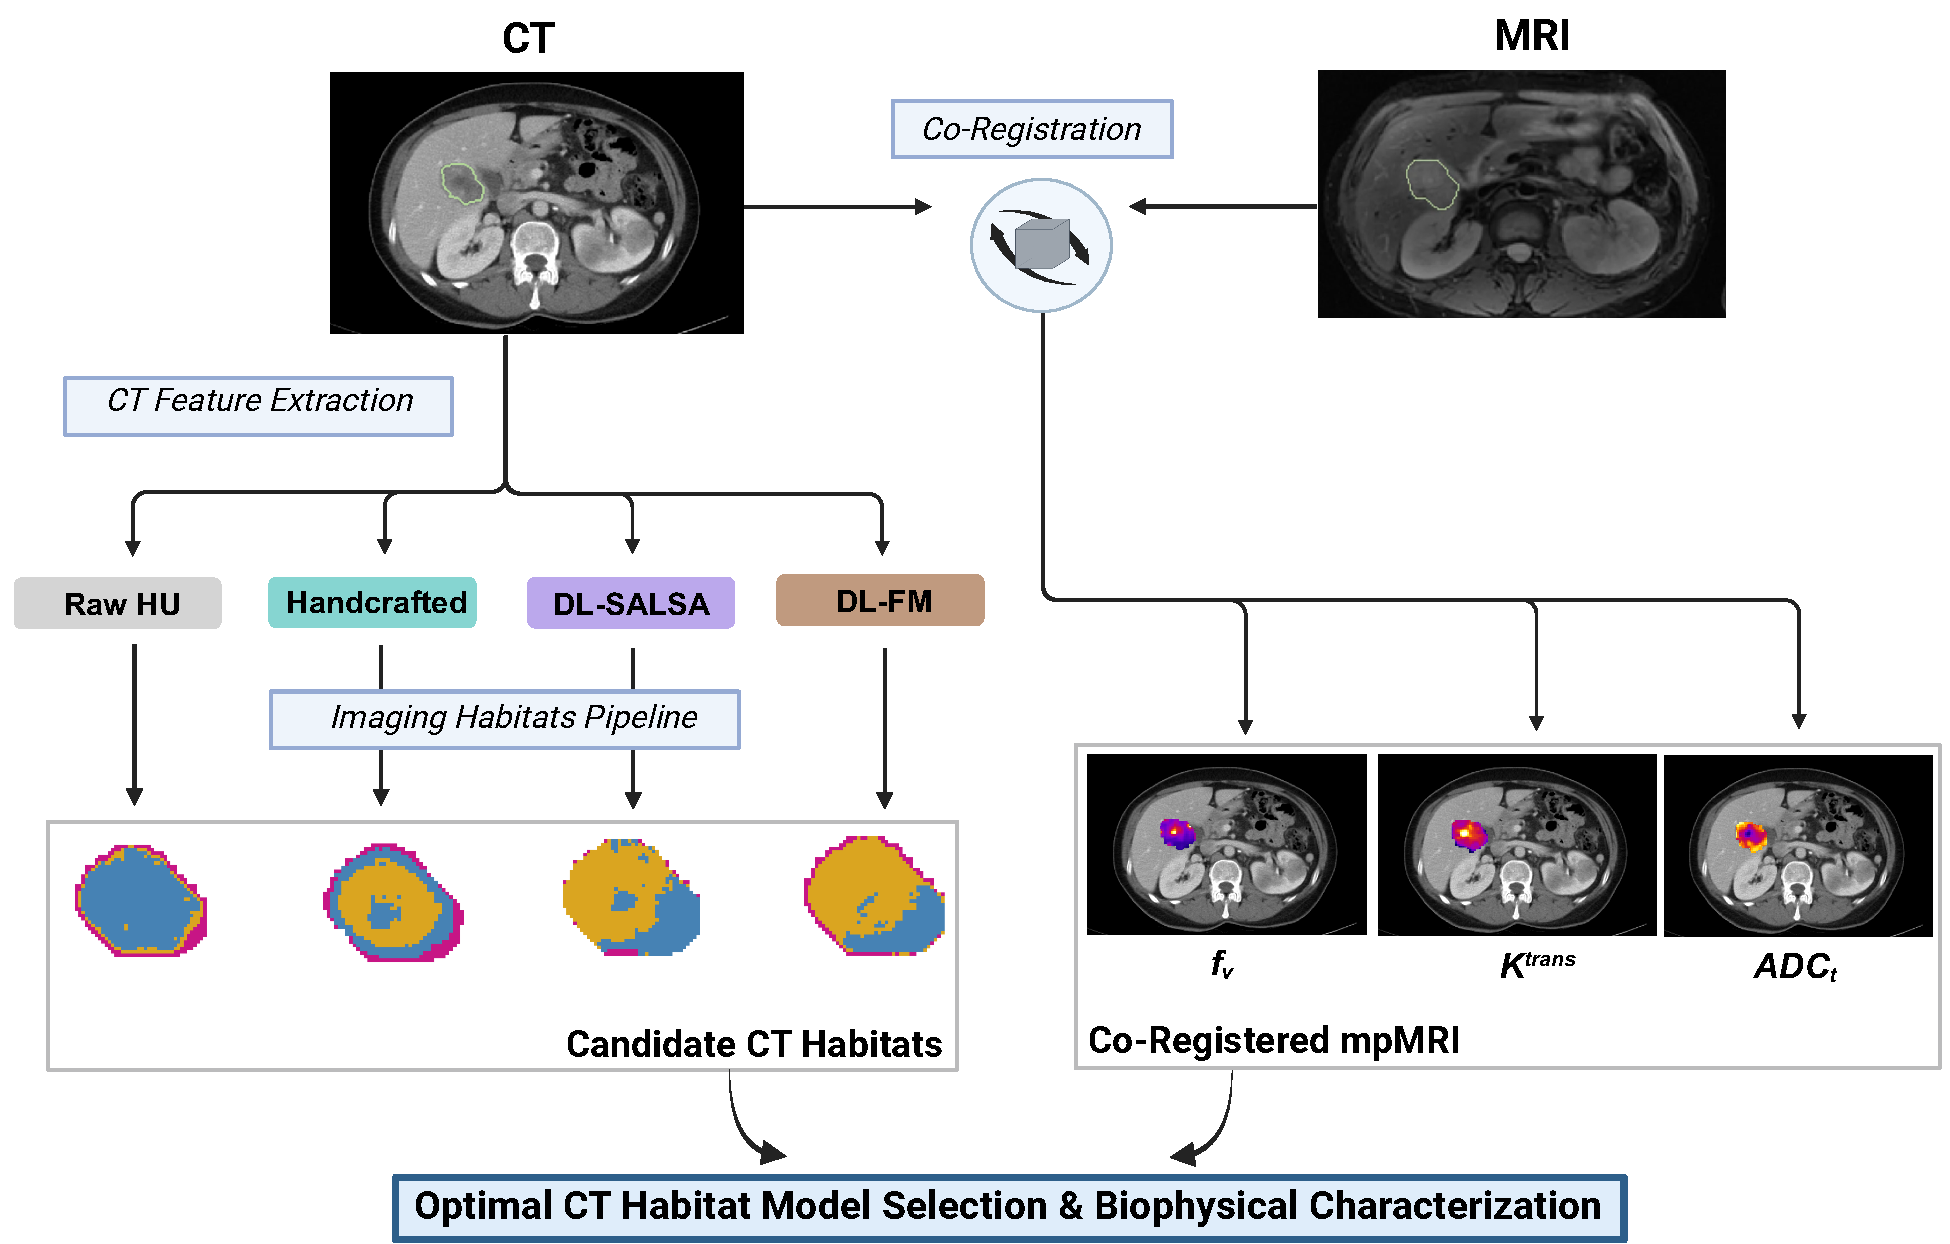
\includegraphics[width=0.95\textwidth]{fig_7_1.pdf}
\caption{Schematic of the mpMRI-anchored CT habitat model development.
CT and MRI scans from the PREDICT cohort were co-registered to T2w
space. Four voxelwise CT feature representations---Raw HU, Handcrafted
Radiomics, DL-SALSA, and DL-FM---were extracted and processed through
the imaging habitats pipeline to generate candidate habitat maps.
Co-registered mpMRI maps (including vascular fraction, $f_v$; capillary
permeability, $K^{trans}$; and tissue apparent diffusion coefficient, $ADC_t$)
provided biophysical reference for model selection. The optimal CT
habitat model was selected based on its ability to spatially separate
tissue properties reflecting cellularity and vascularity (with the three
mpMRI maps shown: ADCt, Ktrans and fv), and further characterized using
additional mpMRI maps. Created with BioRender.com.}
\label{fig:7.1}
\end{figure}

\subsection{CT-mpMRI Co-Registration}\label{ct-mpmri-co-registration}

To enable voxelwise comparison between CT{} and mpMRI, all images were
spatially co-registered to the T2-weighted image, which served as the
fixed reference. This required three registration pipelines: CT{}→T2w,
DWI→T2w, and GRE→T2w. We followed

Images were cropped to a tumor-centered bounding box (5--7 mm margin)
and resampled to 2×2×2 mm isotropic resolution prior to registration.
Registration was performed using NiftyReg in sequential stages: rigid,
affine, then deformable B-spline if alignment improved. Quality was
assessed by Dice similarity coefficient (DSC) between the T2w tumor mask
and the warped mask; the transformation yielding the highest DSC was
retained. Full methodological details are provided in Annex C.

\subsection{CT Feature Extraction}\label{ct-feature-extraction}

Four CT{} representations were evaluated:

\begin{itemize}
\item
  \textbf{Raw Hounsfield units.} The original portal-venous phase CT{}
  images, serving as baseline.
\item
  \textbf{Handcrafted radiomics features.} Voxelwise texture features
  computed using PyRadiomics, based on the 26 precise features
  identified in Chapter 6 (see Section 6.3.2). To avoid clustering on
  redundant information, we removed highly correlated features (Spearman
  \textbar ρ\textbar{} ≥ 0.80), retaining 6 non-redundant features: 10th
  percentile intensity, GLDM dependence entropy, GLDM small dependence
  high gray level emphasis, GLRLM gray level non-uniformity, GLRLM run
  length non-uniformity, and NGTDM coarseness. Correlation analysis is
  detailed in Annex C.
\item
  \textbf{Deep learning features from a liver tumro segmentation model
  (DL-SALSA).} Activations from the penultimate decoder layer of SALSA,
  a 3D nnU-Net trained for liver tumor segmentation (Balaguer-Montero et
  al., 2025).
\item
  \textbf{Deep learning features from a foundation model (DL-FM).}
  Activations from a SegResEncoder foundation model pretrained on
  diverse CT{} datasets using self-supervised learning (Pai et al.,
  2025).
\end{itemize}

All CT{} images were resampled to 1×1×1 mm isotropic resolution prior to
feature extraction. For biological evaluation, the resulting habitat
maps were warped to the T2w reference space (2×2×2 mm) using
nearest-neighbor interpolation.

\subsection{CT Habitat Model Development}\label{ct-habitat-model-development}

\subsubsection{\texorpdfstring{\textbf{7.2.4.1 Clustering
Configuration}}{7.2.4.1 Clustering Configuration}}\label{clustering-configuration}

Habitats were computed using the imaging habitats pipeline described in
Section 5.4, with standard preprocessing: features with high
right-skewness (\textgreater1.0) were log-transformed; all features were
then standardized to zero mean and unit variance. Clustering followed
the two-stage hybrid approach: local GMM clustering within each tumor,
followed by meta-clustering of local centroids to define global
prototypes. The number of habitats was set to K=3, based on the
hypothesis that CT{}-derived clusters could correspond to the dominant
histological compartments of colorectal liver metastases: viable tumor,
necrosis, and fibrosis. The fitted scaler and global prototypes were
saved, enabling application to new data without retraining.

\subsubsection{\texorpdfstring{\textbf{7.2.4.2 CT}{} \textbf{Habitat
Model
Selection}}{7.2.4.2 CT Habitat Model Selection}}\label{ct-habitat-model-selection}

To select the optimal CT{} representation, we evaluated how well each
feature set produced habitats that separate \emph{biologically} distinct
tissue, using the co-registered mpMRI maps as reference. Specifically,
we selected the following three:

\begin{itemize}
\item
  \textbf{ADC\textsubscript{t}} (tissue apparent diffusion coefficient):
  a proxy for cellularity
\item
  \textbf{f\textsubscript{v}} (vascular signal fraction): a measure of
  blood volume
\item
  \textbf{K\textsuperscript{trans}} (volume transfer constant): a
  measure of capillary permeability
\end{itemize}

Both fv and Ktrans were included to capture different aspects of tumor
vascularity---structural vascular density fv versus functional leakiness
and perfusion Ktrans.

For each representation, we computed habitats and extracted the median
value of each mpMRI metric within each habitat for each patient. We
aggregated to patient level (N=10) to avoid pseudo-replication. Habitat
separation was assessed using the Friedman test, with
Kendall\textquotesingle s W as effect size (Kendall \& Smith, 1939;
Tomczak \& Tomczak, n.d.) . To summarize performance across the three
metrics, we computed a biophysical separation score defined as the mean
Kendall\textquotesingle s W across ADCt, fv, and Ktrans. The
representation with the highest biophysical separation score was
selected for further validation.

\subsubsection{\texorpdfstring{\textbf{7.2.4.3 Technical
Validation}}{7.2.4.3 Technical Validation}}\label{technical-validation}

Strong biophysical separation could be spurious if the clustering is
unstable. We therefore evaluated:

\begin{itemize}
\item
  \textbf{Initialization stability.} Mean pairwise Adjusted Rand Index
  across 5 random seeds. High ARI indicates the solution is reproducible
  regardless of initialization.
\item
  \textbf{Data stability.} Mean ARI across 30 bootstrap iterations,
  comparing each resampled model to the full-cohort reference. High ARI
  indicates that habitat definitions are not driven by a few patients.
\item
  \textbf{Spatial coherence.} Moran\textquotesingle s I (spatial
  autocorrelation) and surface-area-to-volume ratio. Biologically
  plausible habitats should form contiguous regions, not scattered
  noise.
\end{itemize}

\subsubsection{\texorpdfstring{\textbf{7.2.4.4 Habitat Characterization
with
mpMRI}}{7.2.4.4 Habitat Characterization with mpMRI}}\label{habitat-characterization-with-mpmri}

Having selected the optimal CT{} representation based on biophysical
separation, we characterized the resulting habitats using the full panel
of mpMRI metrics available in the PREDICT cohort.

Our initial hypothesis was that CT{} habitats would correspond to
histologically defined compartments: necrosis, fibrosis, and viable
tumor. The mpMRI characterization served to test this hypothesis and, if
the correspondence proved incomplete, to build an alternative
interpretive framework based on the tissue properties the habitats
actually captured.

For each of the 13 mpMRI maps (\hyperref[_Ref219812935]{Table 5.2}), we
extracted the median value within each habitat for each patient,
following the same aggregation approach used for model selection.
Differences across the three habitats were assessed using the Friedman
test, with Kendall\textquotesingle s W as effect size. Post-hoc pairwise
comparisons used Wilcoxon signed-rank tests with Benjamini-Hochberg
(Benjamini \& Hochberg, 1995) correction for multiple comparisons within
each metric.

\subsection{Histopathological Validation}\label{histopathological-validation}

To assess whether CT{} habitats correspond to histologically defined
tissue compartments, we applied the trained model to the POEM cohort
(Section 5.1.3). Whole-tumor H\&E sections were digitized and annotated
for viable tumor, necrosis, and fibrosis using a supervised pixel
classifier in QuPath (Bankhead et al., 2017), trained on regions
delineated by the author of this thesis, based on an experienced
pathologist's guidance. Automated annotations were reviewed by the
pathologist for quality assurance. We then performed two experiments:

\begin{itemize}
\item
  \textbf{Qualitative spatial correspondence.} Direct voxel-to-voxel
  co-registration between CT{} and histology was not feasible. We
  therefore evaluated correspondence qualitatively, comparing the
  spatial distribution of CT{} habitats with the architecture visible on
  annotated histology sections.
\item
  \textbf{Correlation with histological tissue percentages}. As an
  exploratory analysis, we computed Spearman correlations between
  whole-tumor habitat proportions and whole-tumor tissue percentages.
\end{itemize}

The primary goal was not to establish quantitative agreement---which
would require spatial co-registration and larger samples---but to
confirm that CT{} habitats exhibit spatial organization consistent with
known histological architecture: viable tumor rims surrounding necrotic
or fibrotic cores.

\section{Results}\label{results-1}

\subsection{Handcrafted Radiomics Yields the Most Biologically Coherent CT Habitats}\label{handcrafted-radiomics-yields-the-most-biologically-coherent-ct-habitats}

\textbf{Co-registration quality.} We first assessed the quality of the
three registration pipelines required for voxelwise CT{}--mpMRI
comparison. The majority of registrations used rigid transformations; no
deformable registration was required. Across 42 tumors, the DWI-to-T2w
registration achieved the highest alignment (median DSC = 0.79, IQR:
0.71--0.84), followed by GRE-to-T2w (median DSC = 0.76, IQR: 0.66--0.85)
and CT{}-to-T2w (median DSC = 0.70, IQR: 0.65--0.78).

\textbf{CT}{} \textbf{Habitat Model Selection.} We compared the four
CT{} representations by their ability to produce habitats that separate
the three pre-specified mpMRI metrics: tissue ADC (cellularity proxy),
vascular fraction (fv), and perfusion (Ktrans).
\hyperref[_Ref219821967]{Figure 7.2} shows examples of CT{} habitats
with the four feature sets. \hyperref[_Ref219821259]{Table 7.1}
summarizes the results.

Handcrafted radiomics achieved the highest biophysical separation score
(mean W = 0.45), driven by strong effects for vascular fraction (W =
0.67, p = 0.005) and perfusion (W = 0.52, p = 0.018). Raw HU showed
moderate separation for cellularity (W = 0.31) but failed to distinguish
vascular phenotypes. DL-SALSA performed moderately on vascular metrics;
DL-FM showed no significant separation on any metric.

Notably, none of the representations achieved strong separation on ADCt,
our primary cellularity proxy. This suggested that CT{} habitats capture
vascular rather than cellular heterogeneity---a finding we examine in
detail in Section 7.3.2.

\textbar{} Comparison of candidate CT{} feature representations

\begin{longtable}[]{@{}
  >{\centering\arraybackslash}p{(\linewidth - 14\tabcolsep) * \real{0.1841}}
  >{\centering\arraybackslash}p{(\linewidth - 14\tabcolsep) * \real{0.0651}}
  >{\centering\arraybackslash}p{(\linewidth - 14\tabcolsep) * \real{0.1189}}
  >{\centering\arraybackslash}p{(\linewidth - 14\tabcolsep) * \real{0.0912}}
  >{\centering\arraybackslash}p{(\linewidth - 14\tabcolsep) * \real{0.1390}}
  >{\centering\arraybackslash}p{(\linewidth - 14\tabcolsep) * \real{0.1227}}
  >{\centering\arraybackslash}p{(\linewidth - 14\tabcolsep) * \real{0.1073}}
  >{\centering\arraybackslash}p{(\linewidth - 14\tabcolsep) * \real{0.1563}}@{}}
\caption{*p \textless{} 0.05 after Bonferroni correction. W =
Kendall\textquotesingle s W effect size.}\tabularnewline
\toprule\noalign{}
\multirow{2}{=}{\centering\arraybackslash \begin{minipage}[b]{\linewidth}\centering
\end{minipage}} &
\multicolumn{2}{>{\centering\arraybackslash}p{(\linewidth - 14\tabcolsep) * \real{0.1841} + 2\tabcolsep}}{%
\begin{minipage}[b]{\linewidth}\centering
\textbf{ADCt}
\end{minipage}} &
\multicolumn{2}{>{\centering\arraybackslash}p{(\linewidth - 14\tabcolsep) * \real{0.2301} + 2\tabcolsep}}{%
\begin{minipage}[b]{\linewidth}\centering
\textbf{Vascular Fraction}
\end{minipage}} &
\multicolumn{2}{>{\centering\arraybackslash}p{(\linewidth - 14\tabcolsep) * \real{0.2300} + 2\tabcolsep}}{%
\begin{minipage}[b]{\linewidth}\centering
\textbf{Ktrans}
\end{minipage}} &
\multirow{2}{=}{\centering\arraybackslash \begin{minipage}[b]{\linewidth}\centering
\textbf{Biophysical Score}
\end{minipage}} \\
& \begin{minipage}[b]{\linewidth}\centering
W
\end{minipage} & \begin{minipage}[b]{\linewidth}\centering
P-value
\end{minipage} & \begin{minipage}[b]{\linewidth}\centering
W
\end{minipage} & \begin{minipage}[b]{\linewidth}\centering
P-value
\end{minipage} & \begin{minipage}[b]{\linewidth}\centering
W
\end{minipage} & \begin{minipage}[b]{\linewidth}\centering
P-value
\end{minipage} \\
\midrule\noalign{}
\endfirsthead
\toprule\noalign{}
\multirow{2}{=}{\centering\arraybackslash \begin{minipage}[b]{\linewidth}\centering
\end{minipage}} &
\multicolumn{2}{>{\centering\arraybackslash}p{(\linewidth - 14\tabcolsep) * \real{0.1841} + 2\tabcolsep}}{%
\begin{minipage}[b]{\linewidth}\centering
\textbf{ADCt}
\end{minipage}} &
\multicolumn{2}{>{\centering\arraybackslash}p{(\linewidth - 14\tabcolsep) * \real{0.2301} + 2\tabcolsep}}{%
\begin{minipage}[b]{\linewidth}\centering
\textbf{Vascular Fraction}
\end{minipage}} &
\multicolumn{2}{>{\centering\arraybackslash}p{(\linewidth - 14\tabcolsep) * \real{0.2300} + 2\tabcolsep}}{%
\begin{minipage}[b]{\linewidth}\centering
\textbf{Ktrans}
\end{minipage}} &
\multirow{2}{=}{\centering\arraybackslash \begin{minipage}[b]{\linewidth}\centering
\textbf{Biophysical Score}
\end{minipage}} \\
& \begin{minipage}[b]{\linewidth}\centering
W
\end{minipage} & \begin{minipage}[b]{\linewidth}\centering
P-value
\end{minipage} & \begin{minipage}[b]{\linewidth}\centering
W
\end{minipage} & \begin{minipage}[b]{\linewidth}\centering
P-value
\end{minipage} & \begin{minipage}[b]{\linewidth}\centering
W
\end{minipage} & \begin{minipage}[b]{\linewidth}\centering
P-value
\end{minipage} \\
\midrule\noalign{}
\endhead
\bottomrule\noalign{}
\endlastfoot
\begin{minipage}[t]{\linewidth}\centering
\begin{quote}
Raw HU
\end{quote}
\end{minipage} & 0.31 & 0.2928 & 0.12 & 0.4894 & 0.04 & 0.6703 &
0.1567 \\
\begin{minipage}[t]{\linewidth}\centering
\begin{quote}
Handcrafted
\end{quote}
\end{minipage} & 0.16 & 0.3281 & 0.67 & 0.0053* & 0.52 & 0.0055* &
0.4500 \\
\begin{minipage}[t]{\linewidth}\centering
\begin{quote}
DL-SALSA
\end{quote}
\end{minipage} & 0.1481 & 0.3808 & 0.4815 & 0.0853 & 0.3457 & 0.0446* &
0.3251 \\
\begin{minipage}[t]{\linewidth}\centering
\begin{quote}
DL-FM
\end{quote}
\end{minipage} & 0.13 & 0.4429 & 0.19 & 0.3889 & 0.13 & 0.2725 &
0.1500 \\
\end{longtable}

To assess whether the three-habitat solution was optimal for the
selected representation, we performed post-hoc sensitivity analyses with
K=2 and K=4. The K=3 solution provided the best balance between
biological interpretability and cluster stability; K=2 merged
biologically distinct vascular phenotypes, while K=4 introduced a
habitat with unstable membership across bootstrap iterations. Results
are detailed in Annex C.

\textbf{Technical validation.} All representations demonstrated high
initialization stability (ARI \textgreater{} 0.96), indicating that the
clustering solution was reproducible regardless of random seed. However,
spatial coherence differed substantially. Handcrafted features produced
spatially contiguous habitats (Moran\textquotesingle s I ≈ 0.80), while
DL-SALSA and DL-FM produced fragmented, "salt-and-pepper" patterns with
low spatial autocorrelation. Full technical validation results are
reported in Annex C.

Based on these findings, handcrafted radiomics was selected as the final
CT{} habitat model.

\begin{figure}[htbp]
\centering
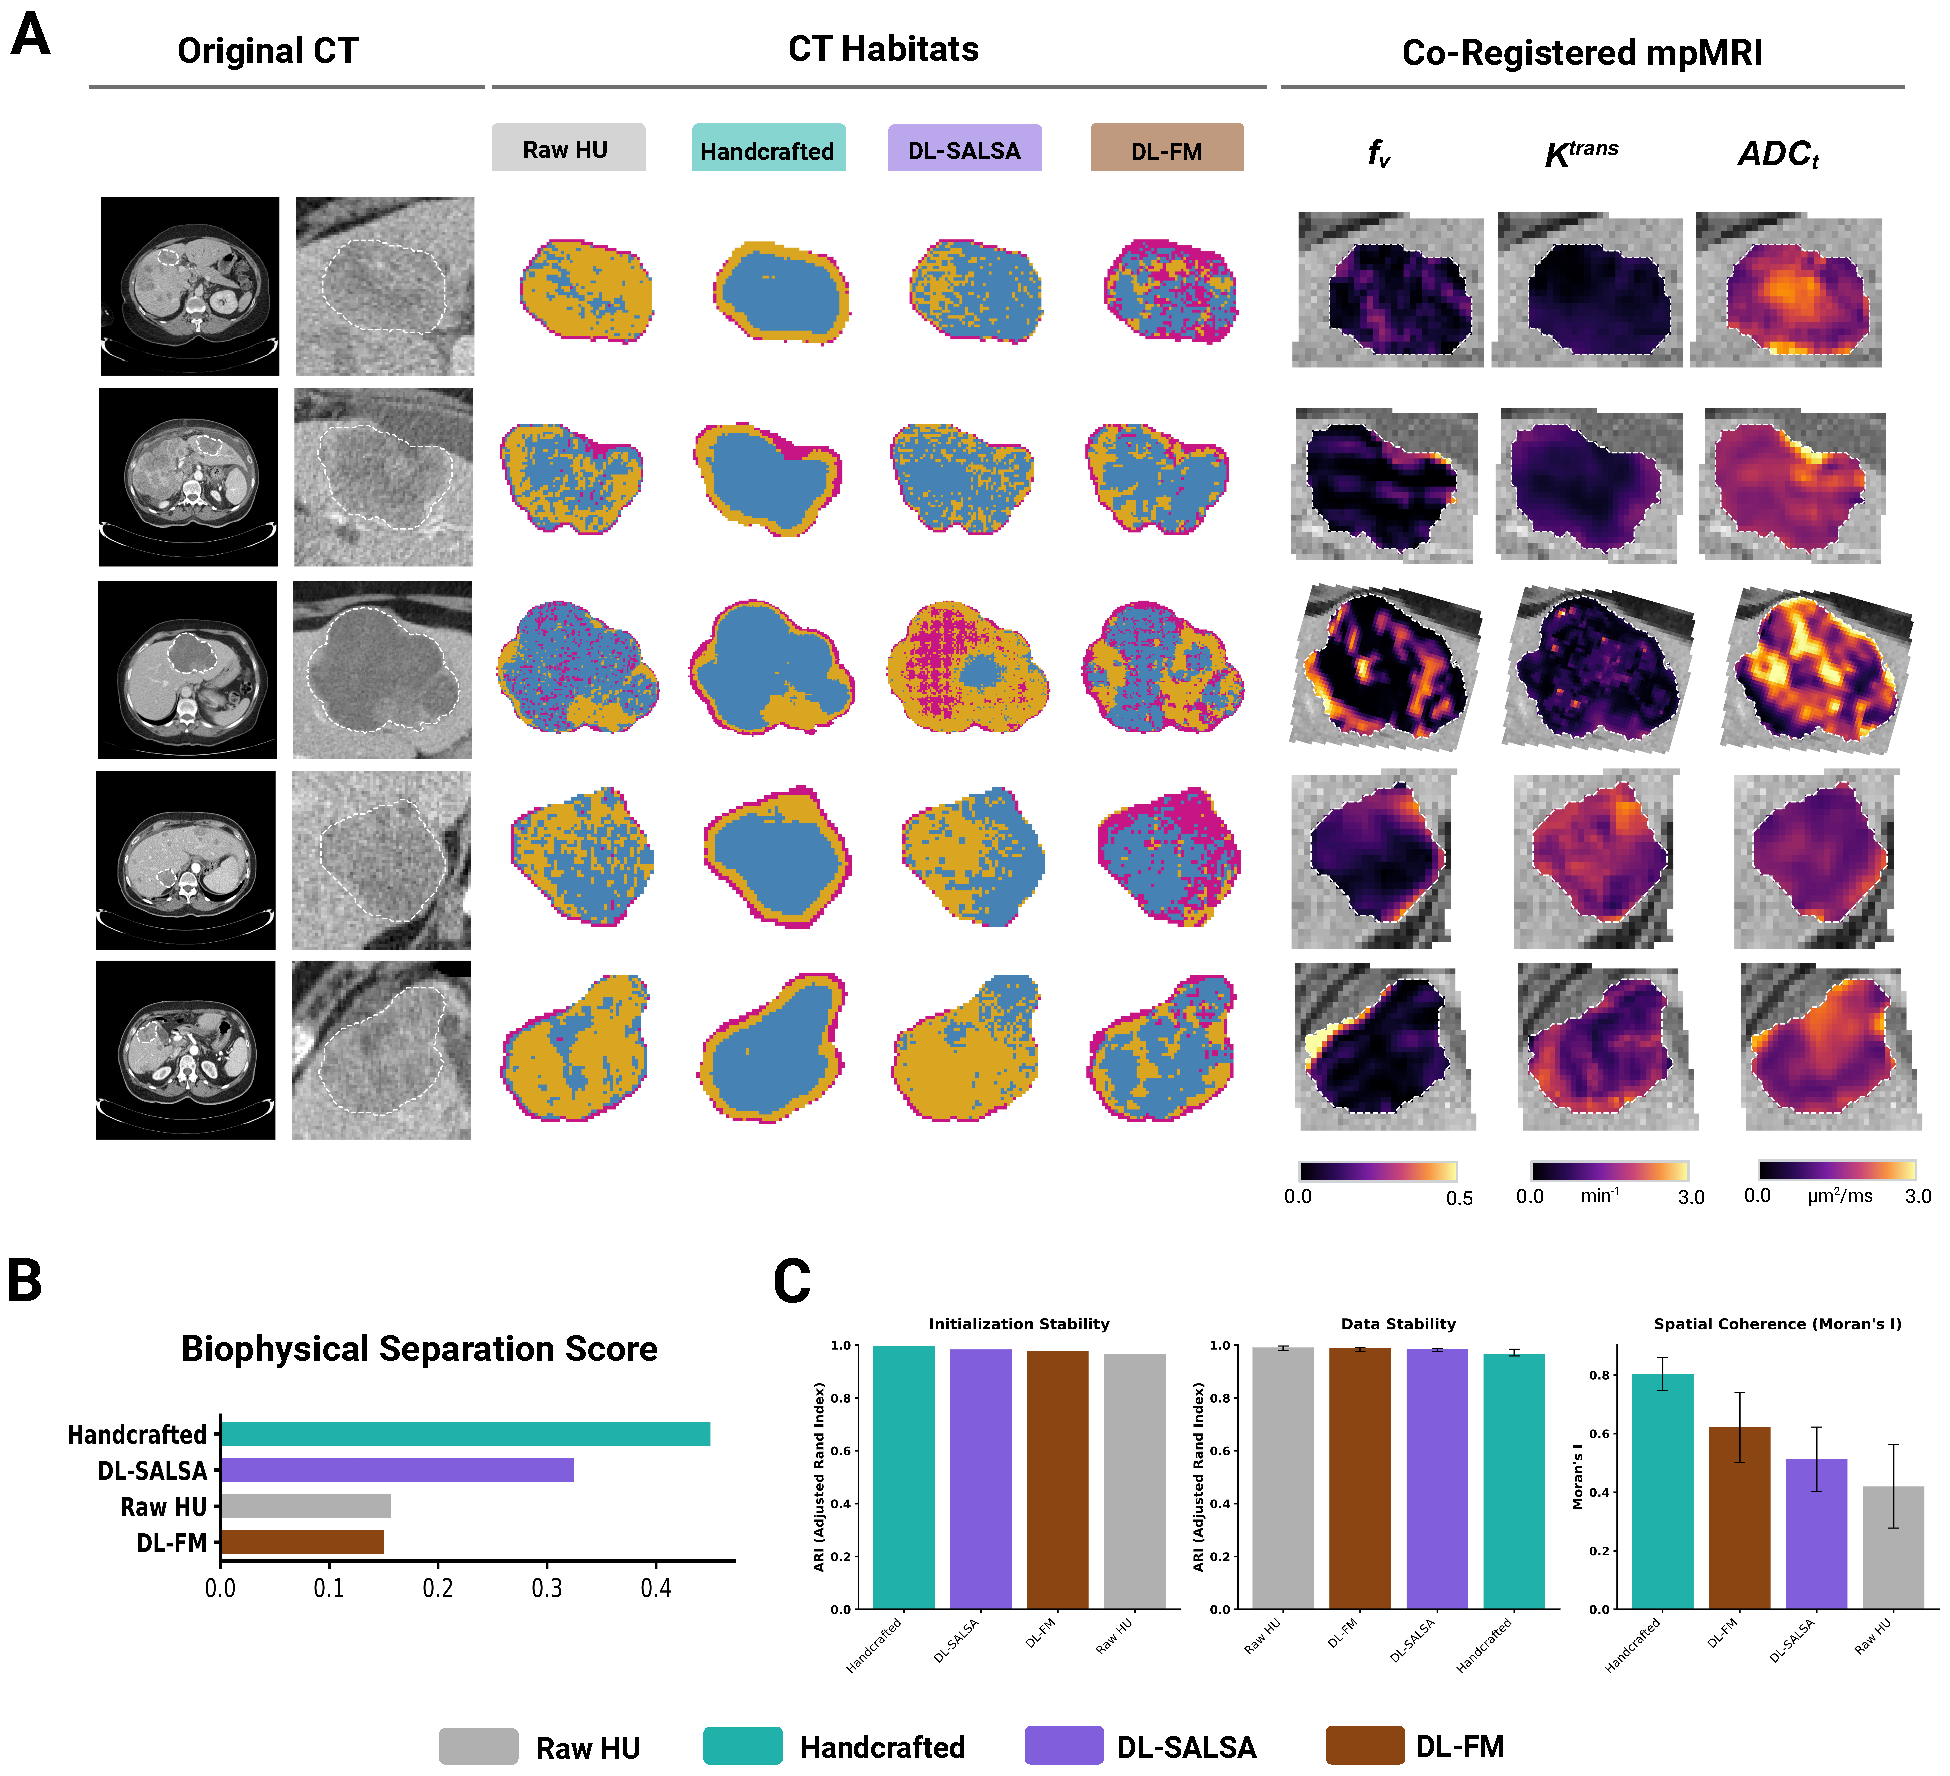
\includegraphics[width=0.95\textwidth]{fig_7_2.pdf}
\caption{Selection of the optimal CT representation.
\textbf{(A)} Representative habitat maps for a single tumor generated by
the four candidate representations (Raw HU, Handcrafted Radiomics,
DL-SALSA, DL-FM), alongside reference mpMRI maps (ADCt, fv, Ktrans).
\textbf{(B)} Biophysical separation performance
(Kendall's W) for each representation across the three
pre-specified mpMRI metrics. Handcrafted radiomics achieved the highest
separation on vascular metrics (fv, Ktrans) but not on cellularity
(ADCt). \textbf{(C)} Technical stability metrics: initialization
stability (ARI across seeds), data stability (bootstrap ARI), and
spatial coherence (Moran's I).}
\label{fig:7.2}
\end{figure}

\subsection{CT Habitats Capture Distinct Vascular and Cellular Phenotypes}\label{ct-habitats-capture-distinct-vascular-and-cellular-phenotypes}

We characterized the three habitats using 13 mpMRI metrics to test
whether they corresponded to the hypothesized histological
compartments---necrosis, fibrosis, and viable tumor
(\hyperref[_Ref219821277]{Table 7.2}). \hyperref[_Ref219821980]{Figure
7.3} shows boxplots for the eight metrics with significant differences
across habitats, plus two cellularity-related metrics (fin, ADCt). Full
results with pairwise significance tests are available in Annex C.

\textbar{} CT{} Habitat Characterization with mpMRI metrics

\begin{longtable}[]{@{}
  >{\centering\arraybackslash}p{(\linewidth - 14\tabcolsep) * \real{0.0649}}
  >{\centering\arraybackslash}p{(\linewidth - 14\tabcolsep) * \real{0.2053}}
  >{\centering\arraybackslash}p{(\linewidth - 14\tabcolsep) * \real{0.1460}}
  >{\centering\arraybackslash}p{(\linewidth - 14\tabcolsep) * \real{0.1196}}
  >{\centering\arraybackslash}p{(\linewidth - 14\tabcolsep) * \real{0.1196}}
  >{\centering\arraybackslash}p{(\linewidth - 14\tabcolsep) * \real{0.1196}}
  >{\centering\arraybackslash}p{(\linewidth - 14\tabcolsep) * \real{0.1124}}
  >{\centering\arraybackslash}p{(\linewidth - 14\tabcolsep) * \real{0.1127}}@{}}
\caption{Patient-level median values for 13 mpMRI-derived biophysical
parameters across the three CT{} habitats (N = 10 patients, 42 tumors).
Vascular parameters (fv, Ktrans, ADCv) show a gradient from H1 to H3;
cellular parameters (ADCt, fin, CD) peak in H2. Significance assessed
using Friedman test with Benjamini-Hochberg correction; effect size
reported as Kendall\textquotesingle s W. BH = Benjamini-Hochberg
correction for multiple comparisons across metrics. W =
Kendall\textquotesingle s W coefficient of concordance (effect size). *p
\textless{} 0.05, **p \textless{} 0.01.}\tabularnewline
\toprule\noalign{}
\multicolumn{2}{@{}>{\centering\arraybackslash}p{(\linewidth - 14\tabcolsep) * \real{0.2702} + 2\tabcolsep}}{%
\multirow{2}{=}{\centering\arraybackslash \begin{minipage}[b]{\linewidth}\centering
\textbf{mpMRI metric}
\end{minipage}}} &
\multirow{2}{=}{\centering\arraybackslash \begin{minipage}[b]{\linewidth}\centering
\textbf{Units}
\end{minipage}} &
\multicolumn{3}{>{\centering\arraybackslash}p{(\linewidth - 14\tabcolsep) * \real{0.3587} + 4\tabcolsep}}{%
\begin{minipage}[b]{\linewidth}\centering
\textbf{Habitats (medians)}
\end{minipage}} &
\multirow{2}{=}{\centering\arraybackslash \begin{minipage}[b]{\linewidth}\centering
\textbf{p-value (BH)}
\end{minipage}} &
\multirow{2}{=}{\centering\arraybackslash \begin{minipage}[b]{\linewidth}\centering
\textbf{Effect Size (W)}
\end{minipage}} \\
& & & \begin{minipage}[b]{\linewidth}\centering
\textbf{H1}
\end{minipage} & \begin{minipage}[b]{\linewidth}\centering
\textbf{H2}
\end{minipage} & \begin{minipage}[b]{\linewidth}\centering
\textbf{H3}
\end{minipage} \\
\midrule\noalign{}
\endfirsthead
\toprule\noalign{}
\multicolumn{2}{@{}>{\centering\arraybackslash}p{(\linewidth - 14\tabcolsep) * \real{0.2702} + 2\tabcolsep}}{%
\multirow{2}{=}{\centering\arraybackslash \begin{minipage}[b]{\linewidth}\centering
\textbf{mpMRI metric}
\end{minipage}}} &
\multirow{2}{=}{\centering\arraybackslash \begin{minipage}[b]{\linewidth}\centering
\textbf{Units}
\end{minipage}} &
\multicolumn{3}{>{\centering\arraybackslash}p{(\linewidth - 14\tabcolsep) * \real{0.3587} + 4\tabcolsep}}{%
\begin{minipage}[b]{\linewidth}\centering
\textbf{Habitats (medians)}
\end{minipage}} &
\multirow{2}{=}{\centering\arraybackslash \begin{minipage}[b]{\linewidth}\centering
\textbf{p-value (BH)}
\end{minipage}} &
\multirow{2}{=}{\centering\arraybackslash \begin{minipage}[b]{\linewidth}\centering
\textbf{Effect Size (W)}
\end{minipage}} \\
& & & \begin{minipage}[b]{\linewidth}\centering
\textbf{H1}
\end{minipage} & \begin{minipage}[b]{\linewidth}\centering
\textbf{H2}
\end{minipage} & \begin{minipage}[b]{\linewidth}\centering
\textbf{H3}
\end{minipage} \\
\midrule\noalign{}
\endhead
\bottomrule\noalign{}
\endlastfoot
ADCₜ & Tissue ADC & μm²/ms & 1.45 & 1.3 & 1.36 & 0.328 & 0.16 \\
ADCᵥ & Vascular ADC & μm²/ms & 16.6 & 16.8 & 17.6 & 0.044* & 0.39 \\
Kₜ & Tissue kurtosis excess & Dimensionless & 0.75 & 0.69 & 0.7 & 0.587
& 0.07 \\
\textbf{fᵥ} & \textbf{Vascular signal fraction} & Normalized & 0.068 &
0.081 & 0.112 & 0.005** & 0.67 \\
T₂ₜ & Tissue T₂ & ms & 81.4 & 100.8 & 82.9 & 0.726 & 0.04 \\
\textbf{D₀} & \textbf{Intrinsic diffusivity} & μm²/ms & 37.5 & 54.1 &
71.6 & 0.001** & 0.84 \\
vCS & Volume-weighted cell size & μm & 24 & 23.6 & 23.9 & 0.529 &
0.09 \\
fᵢₙ & Intracellular fraction & Normalized & 0.46 & 0.5 & 0.48 & 0.113 &
0.28 \\
CD & Cell density & x10\textsuperscript{3} Cells/mm³ & 51.2 & 56.8 &
53.6 & 0.529 & 0.09 \\
\textbf{T₁} & \textbf{T₁} & ms & 1063 & 945 & 911 & 0.019* & 0.49 \\
\textbf{T2\textsuperscript{*}} & \textbf{T2\textsuperscript{*}} & ms &
27.5 & 26.5 & 23.7 & 0.001** & 0.84 \\
\textbf{Kᵗʳᵃⁿˢ} & \textbf{Capillary permeability} & min⁻¹ & 0.41 & 0.52
& 0.51 & 0.018* & 0.52 \\
vₑ & Extracellular-extravascular volume & Normalized & 0.66 & 0.73 &
0.74 & 0.741 & 0.03 \\
\end{longtable}

Vascular parameters showed consistent gradients across habitats.
Vascular fraction (fv) increased monotonically from H1 to H3 (0.068 →
0.112; W = 0.67, p = 0.005), as did vascular ADC. Relaxation times (T2*,
T1) decreased in parallel, consistent with increased blood content and
contrast uptake. However, capillary permeability (Ktrans) did not follow
this gradient---it was highest in H2 (0.52 min⁻¹), not H3 (0.51 min⁻¹),
with both elevated relative to H1 (W = 0.52, p = 0.018). If H3
represented angiogenic tumor tissue, we would expect it to show the
highest Ktrans, since tumor neovessels are typically leaky. The
combination of high fv but moderate Ktrans in H3 suggests partial volume
effects at the tumor-liver interface, where voxels mix tumor tissue with
adjacent normal liver parenchyma---which has mature, less permeable
vasculature.

Cellular parameters showed a different pattern. Metrics related to
cellularity did not follow a simple gradient---instead, H2 emerged as
the most cellular habitat. Tissue ADC was lowest in H2 (1.30 µm²/ms;
pairwise p = 0.029 vs H1), indicating more restricted diffusion.
Intracellular fraction (fin), cell density (CD), and cell size (vCS)
pointed in the same direction: H2 contains the most densely packed
cells. H1, by contrast, showed low-moderate cellularity consistent with
necrotic or fibrotic tissue; H3 showed intermediate values.

\begin{figure}[htbp]
\centering
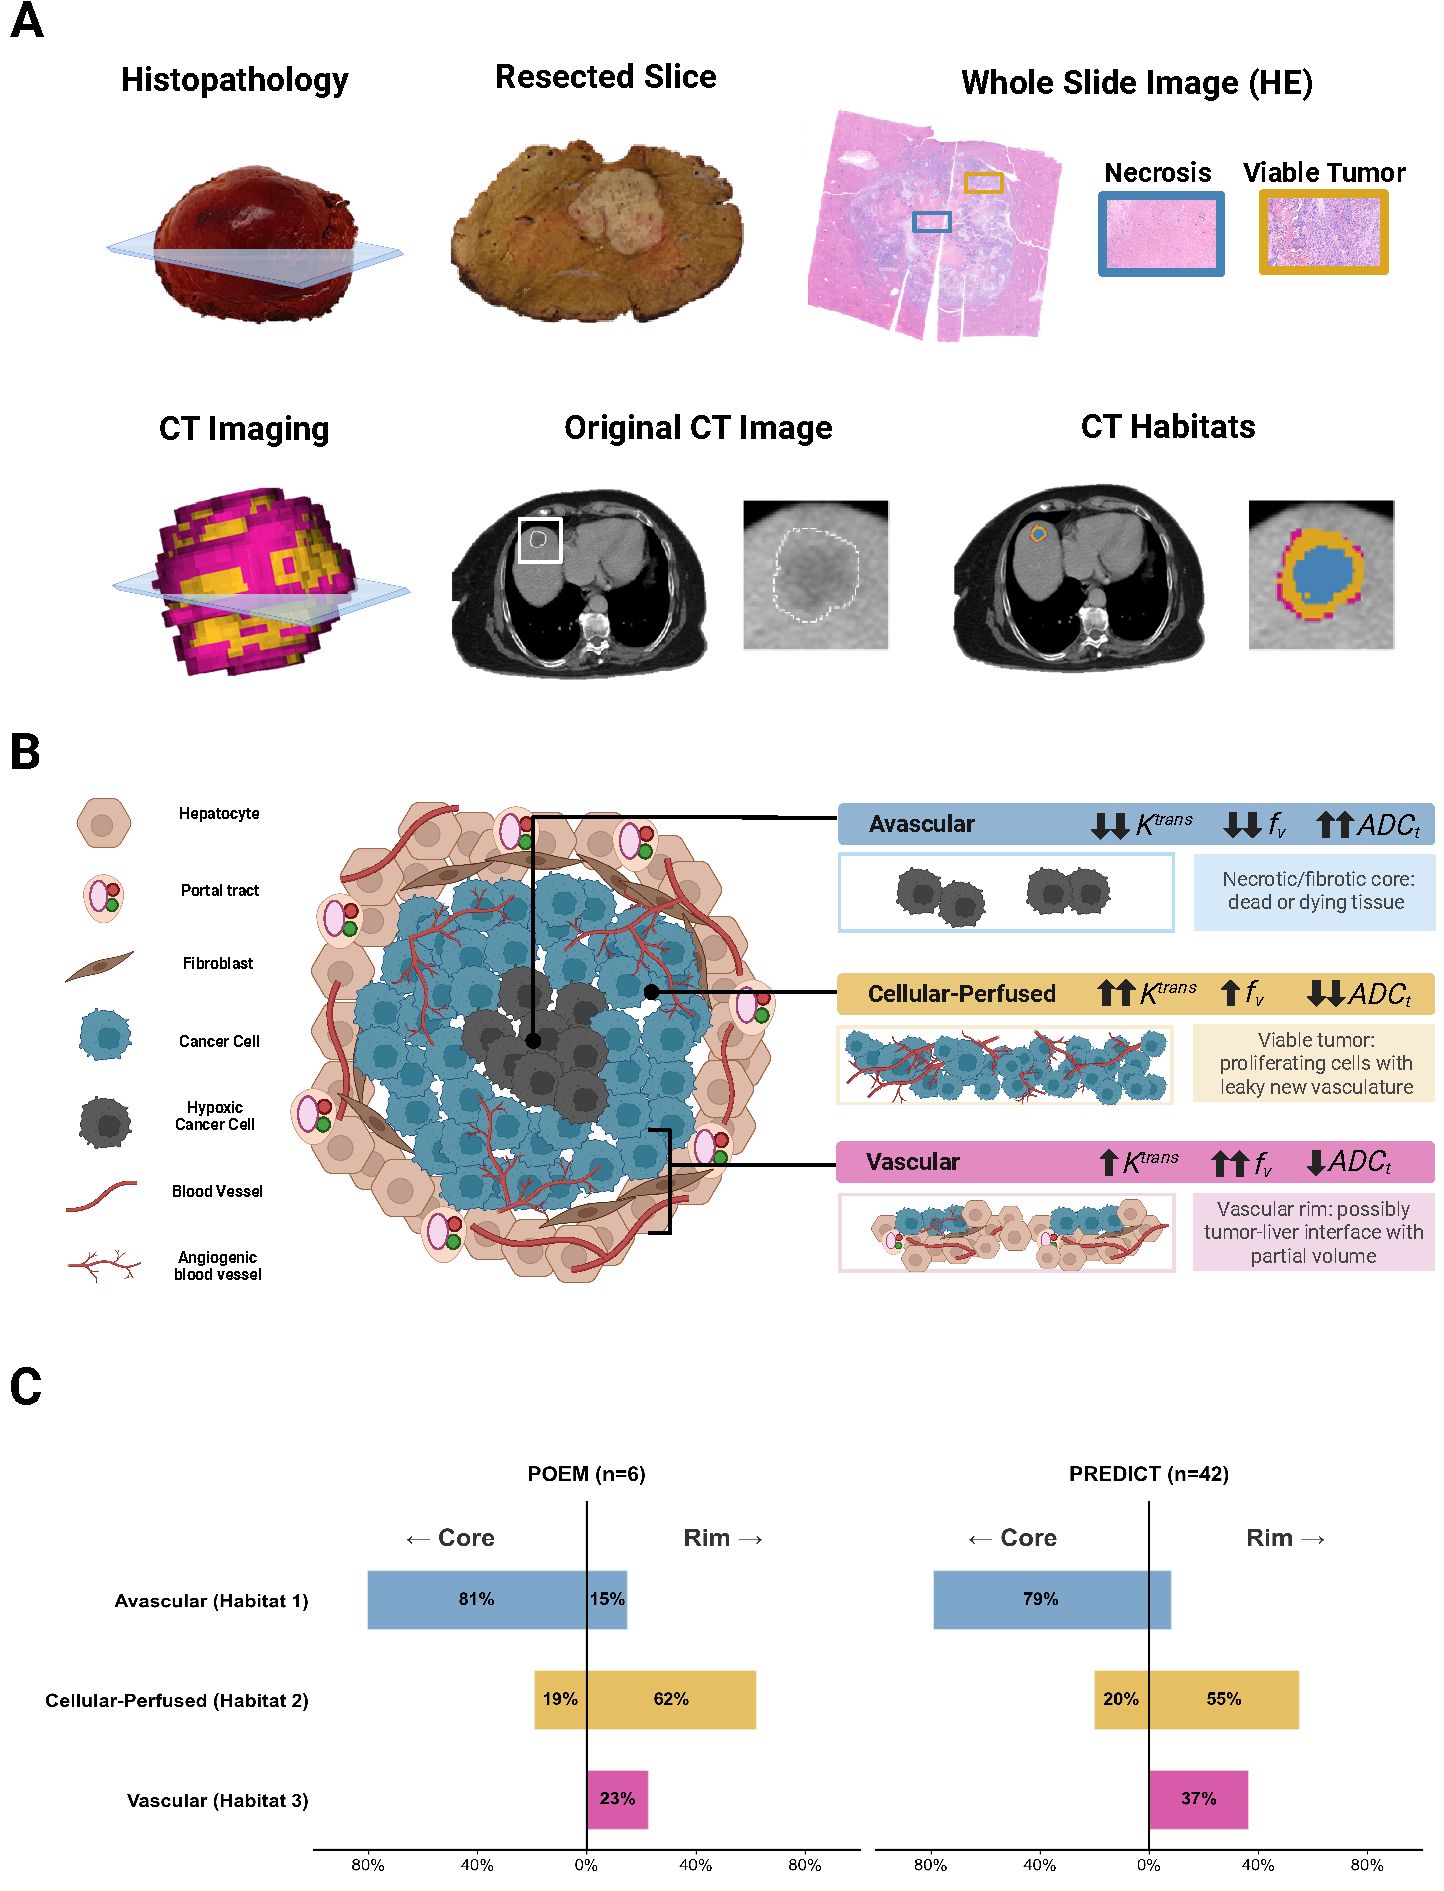
\includegraphics[width=0.95\textwidth]{fig_7_4.pdf}
\caption{Biophysical characterization of CT habitats using mpMRI.
Distribution of eight mpMRI metrics across the three CT habitats (H1:
blue, H2: yellow, H3: pink). Vascular parameters (fv, Ktrans, ADCv, D0)
show gradients from H1 to H3. Cellular parameters (ADCt, fin) show H2 as
the most cellular habitat. Boxplots show patient-level medians (N = 10).
Brackets indicate significant pairwise comparisons (Wilcoxon,
BH-corrected): *p $<$ 0.05, **p $<$ 0.01.}
\label{fig:7.4}
\end{figure}

Based on these profiles, we propose the following biological
interpretation:

\begin{itemize}
\item
  \textbf{Habiat 1: Avascular.} Low vascular fraction, low permeability,
  low-moderate cellularity. Likely contains necrosis, fibrosis, or
  both---CT{} cannot distinguish between them.
\item
  \textbf{Habitat 2: Cellular-Perfused.} Intermediate vascular fraction,
  highest capillary permeability, highest cellularity. Consistent with
  actively proliferating tumor tissue: densely packed viable cells with
  leaky neovessels.
\item
  \textbf{Habitat 3: Vascular.} Highest vascular fraction, moderate
  permeability, moderate cellularity. May capture the tumor-liver
  interface with partial volume from normal liver parenchyma, or a
  vascular-dominant tumor compartment.
\end{itemize}

CT{} habitats thus reflect two aspects of tumor heterogeneity: a
vascular gradient (H1 → H3) and a cellularity peak (H2). The model
distinguishes viable, proliferative tumor (H2) from both the avascular
core (H1) and the vascular interface zone (H3).

\subsection{Spatial Architecture and Histopathological Validation}\label{spatial-architecture-and-histopathologial-validation}

\textbf{Qualitative spatial correspondence.} We applied the trained CT{}
habitat model to the POEM cohort (n = 6) to assess correspondence with
whole-tumor histology. Resected specimens displayed the architecture
characteristic of colorectal liver metastases: central regions of
necrosis and fibrosis surrounded by viable tumor at the periphery
(\hyperref[_Ref219822008]{Figure 7.4}A). CT{} habitat maps captured this
organization---H1 (Avascular) localized to tumor cores, coinciding
mostly with histologically annotated necrosis, while H2
(Cellular-Perfused) and H3 (Vascular) predominated at the periphery,
corresponding to viable tumor margins (\hyperref[_Ref219822008]{Figure
7.4}B).

To quantify this spatial organization, we computed habitat proportions
separately for the tumor rim (2mm outer shell) and core (interior)
across both cohorts (N = 48 tumors: 6 POEM, 42 PREDICT;
\hyperref[_Ref219822008]{Figure 7.4}C). H1 dominated the core (79.4\% ±
2.9\%) but was largely absent from the rim (9.0\% ± 2.3\%). H3 was
concentrated in the rim (35.0\% ± 1.5\%) and virtually absent from the
core (0.4\% ± 0.2\%). H2 showed intermediate localization, enriched in
the rim (56.0\% ± 2.5\%) compared to the core (20.2\% ± 2.9\%). This
pattern was consistent across cohorts: in POEM, cores were 80.5\% H1; in
PREDICT, 79.2\% H1. H3 was absent from POEM cores entirely and
near-absent from PREDICT cores (0.4\%).

\textbf{Correlation with histological tissue percentages}. As an
exploratory analysis, we computed Spearman correlations between
whole-tumor habitat proportions and histological tissue percentages.
Correlations were weak and non-significant (Annex C), reflecting the
scale mismatch between voxel-level imaging and microscopic histology, as
well as CT{}\textquotesingle s inability to distinguish necrosis from
fibrosis within the avascular compartment.

\begin{figure}[htbp]
\centering
\includegraphics[width=0.95\textwidth]{fig_7_3.png}
\caption{Spatial architecture and histopathological validation of CT habitats.
\textbf{(A)} Schematic representation of habitat organization in
colorectal liver metastases. H1 (Avascular, blue) localizes to the tumor
core; H2 (Cellular-Perfused, yellow) represents viable proliferating
tumor; H3 (Vascular, pink) localizes to the periphery at the tumor-liver
interface. \textbf{(B)} Habitat proportions in whole tumor, rim (2mm
outer shell), and core (interior) across both cohorts (POEM n=6, PREDICT
n=42). H1 dominates the core ($\sim$80\%); H2 and H3 dominate
the rim. \textbf{(C)} Representative case from the POEM cohort showing
correspondence between CT habitats and whole-tumor histology. Left:
CT slice with habitat overlay. Right: H\&E section. H1 coincides with
necrotic/fibrotic regions (blue); H2 corresponds to viable tumor at the
periphery (yellow).}
\label{fig:7.3}
\end{figure}

\section{Discussion}\label{discussion-1}

Habitat imaging offers a framework for quantifying intratumor
heterogeneity, but most studies cluster voxels without establishing what
the resulting regions represent biologically. In this chapter, we
addressed this gap by developing an mpMRI-anchored framework for CT{}
habitat discovery. We also addressed a question that has not yet been
studied: which CT{} representation produces the most biologically
coherent habitats? Using co-registered mpMRI as a proxy for tissue
cellularity and vascularity, we compared four CT{} representations and
selected the one whose habitats best separated biologically distinct
tissue phenotypes. We then validated the spatial organization of these
habitats against whole-tumor histopathology.

Handcrafted features outperformed deep learning embeddings for habitat
computation. This was unexpected: foundation models trained on large
CT{} datasets encode rich information, and one might assume they would
produce superior results. However, for unsupervised voxelwise
clustering, stability and spatial coherence matter more than
representational capacity. Deep learning features produced fragmented
patterns while handcrafted features produced contiguous regions aligned
with biological gradients. We note that we did not fine-tune the
foundation model or task-specific embeddings for this application---with
domain-specific optimization, learned representations might perform
better. In Section 9.3. we discuss further the use of handcrafted
features in the era of deep learning.

The mpMRI characterization showed that CT{} habitats mostly reflect
vascular architecture. This is not surprising given that we used
contrast-enhanced portal-venous phase CT{}, where signal intensity
directly reflects contrast uptake and thus tissue perfusion. Our
interpretation of the three habitats was: avascular tissue (H1) with low
fv/Ktrans; a cellular-perfused habitat (H2) towards the rim with highest
Ktrans and celullarity indicating possible viable cancer, and finally a
vascular rim (H3) with highest fv and moderate-high Ktrans. The
fv/Ktrans dissociation in H3 has a plausible explanation: high vascular
fraction but moderate permeability is consistent with the tumor-liver
interface, where voxels mix tumor with normal liver parenchyma that has
mature, less leaky vessels.

The spatial analysis confirmed biological plausibility. Across 48 tumors
from two independent cohorts, H1 dominated tumor cores
(\textasciitilde80\%) while H2 and H3 were enriched at the rim (56\% and
35\%, respectively). This architecture---avascular interior,
vascularized periphery---matches the known histology of colorectal liver
metastases, where viable tumor surrounds a necrotic or fibrotic core
{[}Poultsides et al., 2012; Van den Eynden et al., 2013{]}. Our initial
hypothesis---that CT{} habitats would map onto necrosis, fibrosis, and
viable tumor as discrete categories---was not fully supported. CT{}
reliably separates vascularized from avascular tissue, but within the
avascular core it cannot distinguish necrosis from fibrosis. Both are
hypovascular, lack contrast enhancement, and exhibit similar texture on
portal-venous imaging.

This study presented several limitations. The first one and most
important: habitat labels represent the dominant phenotype for each
voxel. In practice, each voxel (which has an average size of one cubic
millimeter) contains several tissue phenotypes at once. The GMM
clustering assigns each voxel a probability distribution across all
three habitats and we report the maximum-probability assignment. This
discretization loses information---a voxel with 40\% probability for H1
and 35\% for H2 is assigned to H1. Despite this inherent uncertainty,
the spatial segregation is clear: avascular tissue dominates the core,
vascular tissue dominates the rim.

Moreover, sample sizes were small (N = 10 PREDICT, N = 6 POEM),
reflecting the difficulty of acquiring co-registered multimodal imaging
and whole-tumor histology. CT{}-mpMRI registration introduces
uncertainty that propagates into habitat analyses although our median
accuracy (DSC 0.70--0.79) compares favorably with recent benchmarks
{[}Demir et al., 2025{]}. The biological interpretation of H3 as
tumor-liver interface is plausible but not proven---alternative
explanations such as a stromal-rich compartment cannot be excluded.
Finally, histopathological validation was qualitative since voxel-wise
co-registration between CT{} and histology was not feasible.

Despite these limitations, the findings have practical relevance. CT{}
is widely available, reproducible, and already part of standard
oncologic care. If CT{} habitats can stratify patients by tumor vascular
architecture, they could inform treatment decisions without additional
imaging. The distinction between vascularized and avascular compartments
is clinically meaningful: vascularized tissue is more likely to respond
to systemic therapy, while avascular cores may indicate resistance.
Whether habitat-derived metrics predict treatment response or survival
is tested in Chapter 8.

\section{Summary}\label{summary-1}

We developed and validated an mpMRI-anchored CT{} habitat model for
colorectal liver metastases. The central question was whether CT{}
habitats can capture the dominant tissue phenotypes of these tumors.
Using co-registered multiparametric MRI as biological reference and
whole-tumor histopathology for validation, we found that CT{} habitats
reflect vascular architecture---but not discrete histological
categories.

\textbf{Key Points:}

\begin{itemize}
\item
  Handcrafted radiomics features yield the most biologically coherent
  habitats. Comparing four CT{} representations (raw HU, handcrafted
  radiomics, DL-SALSA, DL-FM), handcrafted texture features produced
  habitats with the strongest separation of mpMRI-derived vascular
  parameters and the highest spatial coherence.
\item
  CT{} habitats capture vascular heterogeneity, not discrete
  histological compartments. The three habitats represent an avascular
  core (H1), a cellular-perfused zone with leaky neovessels (H2), and a
  vascular rim likely reflecting the tumor-liver interface (H3). CT{}
  cannot distinguish necrosis from fibrosis within the avascular
  compartment.
\item
  Spatial architecture is biologically plausible and consistent across
  cohorts. H1 dominates tumor cores (\textasciitilde80\%); H2 and H3
  dominate the rim. This organization matches the known histology of
  colorectal liver metastases and was validated against whole-tumor
  histopathology in resected specimens.
\end{itemize}



  \cleardoublepage
  \chapter{Clinical Relevance of CT Habitats}\label{clinical-relevance-of-ct-habitats}\label{ch:8}

In Chapter~\ref{ch:7}, we developed an mpMRI-anchored CT habitat model that
segments colorectal liver metastases into three biologically meaningful
compartments: avascular core, cellular-perfused viable tumor, and
vascular rim. Histopathological validation confirmed that this spatial
architecture reflects genuine tumor biology. In this chapter, we address
the central follow-up question: Do these biologically-grounded habitats
provide clinical value beyond standard imaging biomarkers?

\textbf{Contributions:}

\begin{itemize}
\item
  We assess whether habitat-derived metrics predict survival
  independently of tumor volume across two clinical contexts: resectable
  disease treated with curative-intent surgery (TCIA, n=189) and
  unresectable disease treated with palliative systemic therapy (VHIO,
  n=344).
\item
  We evaluate how treatment context modifies prognostic value, testing
  whether habitat metrics are informative after neoadjuvant chemotherapy
  (TCIA) and with anti-angiogenic therapy (VHIO).
\item
  We test whether prognostic signal concentrates at specific spatial
  locations, comparing rim, core, and whole-tumor metrics.
\item
  We explore whether longitudinal habitat changes during treatment
  capture response biology that RECIST classification misses, focusing
  on the ambiguous stable disease category.
\end{itemize}

\begin{quote}
The work presented in Chapters 7 and 8 forms the basis of a manuscript
currently in preparation.
\end{quote}

\section{Rationale}\label{rationale-2}

Tumor volume is the dominant imaging biomarker in oncology. Together
with anatomical location, it determines resectability and guides the
choice between curative surgery and palliative systemic therapy. RECIST
criteria \citep{eisenhauerNewResponseEvaluation2009}, which inform treatment decisions
across solid tumors, define response and progression primarily through
size change. This framework works reasonably well when tumors shrink or
grow substantially ---but there are moments during treatment when
changes in size are not informative

The limitation is not volume itself but what volume ignores: the
internal composition of the tumor. A 30 cm³ metastasis that is 80\%
necrotic differs fundamentally from one that is 80\% viable tumor---yet
both receive identical volumetric assessment. This matters for two
clinical problems. First, response assessment: a tumor that neither
shrinks nor grows might be genuinely controlled by treatment, or it
might be slowly progressing. Survival outcomes among volumetrically
similar patients vary widely, yet current imaging cannot distinguish
these scenarios. Second, treatment selection: many patients do not
respond as expected to first-line therapy, and we lack imaging tools to
predict who will benefit from which regimen. Both problems---assessing
response and selecting treatment---could benefit from imaging biomarkers
that characterize tumor heterogeneity beyond size.

Habitat imaging offers a potential solution. By segmenting tumors into
spatially distinct subregions with different imaging phenotypes,
habitats capture the heterogeneity information that volume discards. In
Chapter 7, we established that CT habitats in colorectal liver
metastases reflect vascular architecture: an avascular compartment
representing necrotic or fibrotic tissue, a cellular-perfused
compartment representing viable tumor, and a vascular rim at the
tumor-liver interface. If these phenotypes have prognostic relevance,
habitat-derived metrics should predict survival independently of
volume---and potentially discriminate outcomes among volumetrically
similar patients.

This chapter tests these hypotheses across two cohorts with
complementary clinical contexts:

TCIA cohort (n=189, resectable disease): Patients underwent hepatic
resection with curative intent; 60\% received neoadjuvant chemotherapy.
We ask: Does neoadjuvant treatment alter habitat composition? Do
post-treatment habitat patterns predict survival? We hypothesize that
treatment remodels tumor composition in ways detectable by CT, and
that spatial heterogeneity at the invasive rim will carry prognostic
information beyond what volume provides.

VHIO cohort (n=344, unresectable disease): Patients received first-line
systemic therapy---chemotherapy alone, chemotherapy plus bevacizumab, or
chemotherapy plus targeted agents. We ask: Do baseline habitat metrics
predict survival? Does prognostic value depend on treatment type and
molecular context? We hypothesize that for cytotoxic chemotherapy, where
response manifests as tumor shrinkage, volume will dominate. For
anti-angiogenic therapy, where treatment slows growth without
necessarily shrinking tumors, spatial heterogeneity at the rim may
capture treatment-relevant biology that volume cannot.

A subset of VHIO patients (n=38) had paired baseline and follow-up
imaging, allowing us to ask a third question: Does the direction of
habitat change during treatment predict outcomes beyond what RECIST
categories provide? If rim heterogeneity captures treatment response,
then the direction of rim entropy change may differ systematically
between responders and progressors.

\section{Methods}\label{methods-2}

\subsection{Patient Cohorts}\label{patient-cohorts-2}

Two independent cohorts were analyzed (\Cref{fig:8.1}A, \Cref{tab:clinical_characteristics}). The TCIA cohort included
189 patients with resectable colorectal liver metastases from a publicly
available dataset. All patients underwent hepatic resection with
curative intent; 115 (60.8\%) received neoadjuvant chemotherapy prior to
surgery. CT imaging was acquired pre-surgery, representing
post-neoadjuvant status in treated patients and treatment-naive status
in untreated patients.

The VHIO cohort included 344 patients with unresectable metastatic
colorectal cancer treated at Vall d\textquotesingle Hebron Institute of
Oncology. All patients received first-line systemic therapy:
chemotherapy alone (n=122), chemotherapy plus bevacizumab (n=133), or
chemotherapy plus targeted therapy (n=69). CT imaging was acquired at
baseline (pre-treatment) for all patients; a subset of 38 patients had
paired follow-up imaging for longitudinal analysis. RAS mutation status
was available for 331 patients (96\%): 136 RAS wild-type, 195 RAS
mutant. Inclusion criteria and image preprocessing for both cohorts are
detailed in Section 5.1.

\subsection{Habitat Computation}\label{habitat-computation}

CT habitats were computed using the biologically-anchored model
developed in Chapter~\ref{ch:7} (Section 7.3.1). Briefly, six handcrafted
features were computed from contrast-enhanced CT (portal phase) and
clustered using a Gaussian mixture model (K=3) in two steps (hybrid mode
in the imaging habitats pipeline, see Section 5.2). The handcrafted
representation was selected over alternatives (raw HU, deep learning
features) based on its superior ability to separate biologically
distinct tissue compartments as measured by co-registered
multiparametric MRI.

This produced three habitats (\Cref{fig:8.1}B):
the avascular habitat (corresponding to necrotic-like or poorly perfused
tissue with low cellularity), the cellular-perfused habitat (highest
cellularity and perfusion, corresponding to viable tumor), and the
vascular habitat (moderate cellularity and high vascularity). The
vascular habitat may partly reflect partial volume effects at the
tumor-liver interface. The biologically-anchored approach ensured that
habitats captured cellular and vascular heterogeneity validated against
ground truth rather than arbitrary clusters.

\subsection{Habitat-Derived Quantitative Metrics}\label{habitat-derived-quantitative-metrics-1}

Quantitative metrics were derived at three spatial scales: whole tumor,
rim (outer 2mm), and core (tumor interior)
(\Cref{fig:8.1}C).

For each scale, we computed habitat proportions (fraction of voxels
assigned to each habitat) and Shannon entropy (diversity of habitat
composition). Higher entropy indicates a more heterogeneous mixture of
habitats; lower entropy indicates dominance by a single habitat. Tumor
volume was computed as the sum of tumor voxels multiplied by voxel
spacing. These metrics follow the definitions in Section 5.2.3. For
patients with multiple liver metastases, metrics were aggregated across
lesions using volume-weighted averaging, giving greater weight to larger
lesions.

\begin{figure}[htbp]
\centering
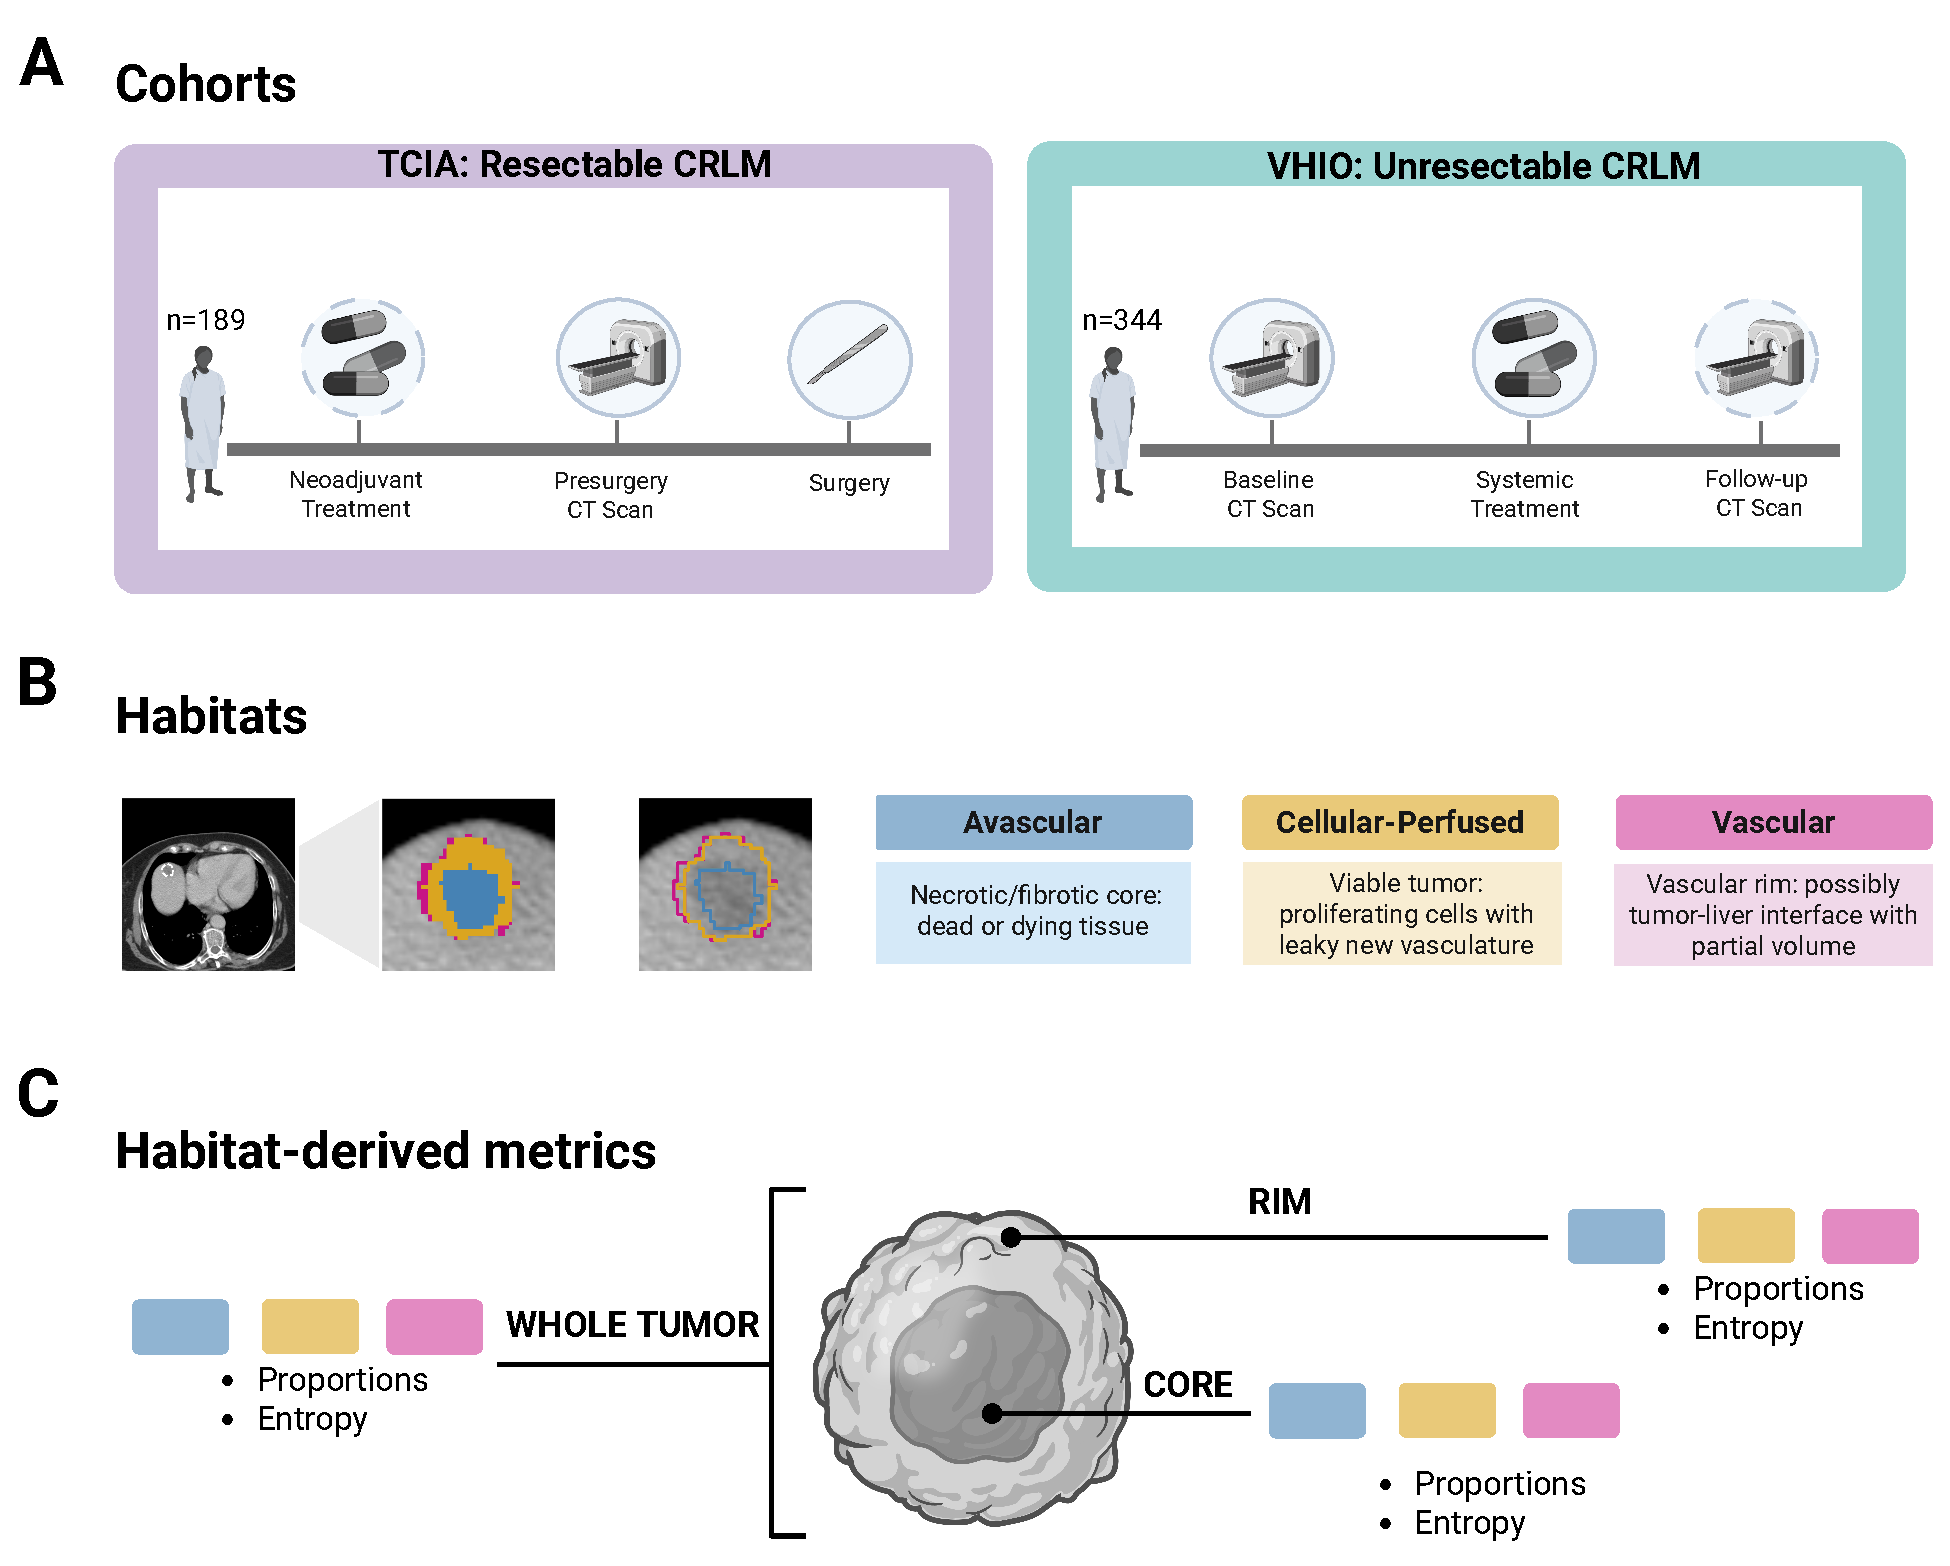
\includegraphics[width=0.95\textwidth]{fig_8_1.pdf}
\caption[Clinical validation study design]{Clinical validation study design.
\textbf{(A)} Two independent cohorts with distinct clinical scenarios.
TCIA (n=189): resectable colorectal liver metastases, CT acquired
pre-surgery (60.8\% received neoadjuvant chemotherapy). VHIO (n=344):
unresectable metastatic colorectal cancer receiving first-line systemic
therapy, CT acquired at baseline; a subset (n=38) had paired follow-up
imaging for longitudinal analysis. \textbf{(B)} CT habitats derived
from the biologically-anchored model (Chapter 7). The avascular habitat
(blue) dominates tumor cores. The cellular-vascular habitat (yellow) and
vascular habitat (red) enrich at the invasive rim. The vascular habitat
may partly reflect partial volume effects at the tumor-liver interface.
\textbf{(C)} Habitat-derived quantitative metrics computed at three
spatial scales (whole tumor, rim, core): habitat proportions and Shannon
entropy. Tumor volume computed as sum of tumor voxels $\times$ voxel spacing.}
\label{fig:8.1}
\end{figure}
For patients with multiple lesions, metrics were aggregated using
volume-weighted averaging. Created with BioRender.com.

\subsection{Statistical Analyses}\label{statistical-analyses}

Group comparisons used Mann-Whitney U tests \citep{mannTestWhetherOne1947} with
false discovery rate (FDR) correction for multiple comparisons
\citep{benjaminiControllingFalseDiscovery1995}.

Survival analyses used Cox proportional hazards regression \citep{coxRegressionModelsLifeTables1972}
in a two-stage approach. Stage 1 screened all variables in univariable
models, retaining those with p\textless0.10. Stage 2 fitted a
multivariable model with retained variables. Hazard ratios (HR) are
reported per standard deviation increase. Model discrimination was
assessed using Harrell\textquotesingle s C-index \citep{harrellMULTIVARIABLEPROGNOSTICMODELS1996}.
The proportional hazards assumption was tested using Schoenfeld
residuals \citep{schoenfeldPartialResidualsProportional1982}. Kaplan-Meier curves \citep{kaplanNonparametricEstimationIncomplete1958} were generated using median splits, with differences assessed by
log-rank test \citep{petoDesignAnalysisRandomized1976}.

Statistical analyses used Python 3.10 with lifelines 0.27
\citep{davidson-pilonLifelinesSurvivalAnalysis2019} and scipy 1.11. Significance was set at
p\textless0.05.

\section{Results}\label{results-2}

\subsection{Patient characteristics}\label{patient-characteristics}

Clinical characteristics of both cohorts are summarized in
\Cref{tab:clinical_characteristics}. The TCIA cohort included 189
patients with resectable colorectal liver metastases who underwent
hepatic resection with curative intent; 115 (60.8\%) received
neoadjuvant chemotherapy prior to surgery. The VHIO cohort included 344
patients with unresectable disease receiving first-line systemic
therapy. VHIO patients had higher liver tumor burden (median 32.4 cm³ vs
10.7 cm³) and more metastases per patient (median 3 vs 2), consistent
with their more advanced disease stage. Overall survival was longer in
TCIA (median 67.1 months) than VHIO (median 19.1 months), reflecting the
curative versus palliative treatment intent.



\begin{table}[ht]
    \centering
    \small
    \caption[Clinical characteristics of the TCIA and VHIO cohorts]{%
        \textbf{Clinical characteristics of the TCIA and VHIO cohorts.}%
        TCIA patients had resectable disease treated with curative-intent surgery; VHIO patients had unresectable disease treated with palliative systemic therapy. IQR = interquartile range; OS = overall survival; DFS = disease-free survival; PFS = progression-free survival.}
    \label{tab:clinical_characteristics}
    \begin{tabular}{@{} p{8cm} c c @{}}
        \toprule
        \textbf{Variables} & \textbf{TCIA (n=189)} & \textbf{VHIO (n=344)} \\
        \midrule
        \textbf{Age} [years, Median(range)] & 61 (30 -- 88) & 69 (32 -- 88) \\ \addlinespace
        \textbf{Sex} [n (\%)] & & \\
        \quad Male & 111 (58.7) & 205 (59.6) \\
        \quad Female & 78 (41.3) & 139 (40.4) \\ \addlinespace
        \textbf{Primary Tumor Location} [n (\%)] & & \\
        \quad Right & & 139 (40.4) \\
        \quad Left & & 183 (53.2) \\
        \quad Rectum & & 17 (4.9) \\
        \quad Unknown & 189 (100) & 5 (1.5) \\ \addlinespace
        \textbf{RAS Status} [n (\%)] & & \\
        \quad Wild-type & & 136 (39.5\%) \\
        \quad Mutant & & 195 (56.7\%) \\
        \quad Unknown & & 13 (3.8\%) \\ \addlinespace
        \textbf{Synchronous CRLM} [n(\%)] & 104 (55.0) & 277 (80.5) \\ \addlinespace
        \textbf{Extrahepatic Disease} [n(\%)] & 15 (7.9) & 203 (59.0) \\ \addlinespace
        \textbf{No. of liver metastases per patient} & 2.0 (1.0, 3.0) & 3.0 (2.0, 7.0) \\
        \quad [Median (IQR)] & & \\ \addlinespace
        \textbf{Median liver metastasis size} & 3.2 (1.2, 10.9) & 5.1 (2.0, 15.0) \\
        \quad [cm$^3$, Median (IQR)] & & \\ \addlinespace
        \textbf{Liver Disease Volume} & 10.7 (4.1, 32.8) & 32.4 (6.8, 180.3) \\
        \quad [cm$^3$, Median (IQR)] & & \\ \addlinespace
        \textbf{First-line Treatment Type} [n (\%)] & -- & \\
        \quad Chemotherapy Only & & 122 (35.5) \\
        \quad Chemotherapy + Antiangiogenic & & 133 (38.7) \\
        \quad Chemotherapy + Targeted & & 69 (20.1) \\
        \quad Other & & 20 (5.8\%) \\ \addlinespace
        \textbf{Neoadjuvant chemotherapy} [n (\%)] & 115 (60.8) & -- \\ \addlinespace
        \textbf{Progression Free Survival} & -- & 8.9 (5.0, 15.3) \\
        \quad [months, Median (IQR)] & & \\ \addlinespace
        \textbf{Overall Survival} & 67.1 (34.4, 97.5) & 19.1 (11.1, 32.8) \\
        \quad [months, Median (IQR)] & & \\ \addlinespace
        \textbf{Disease Free Survival} & 22.3 (9.4, 69.3) & 8.9 (5.0, 15.3) \\
        \quad [months, Median (IQR)] & & \\
        \bottomrule
    \end{tabular}
\end{table}



\subsection{Habitat Characteristics Across Cohorts}\label{habitat-characteristics-across-cohorts}

We assessed whether CT habitats showed consistent spatial patterns and
how they related to tumor volume.

\textbf{Spatial architecture.} Despite differences in tumor burden and
clinical setting, both cohorts showed the same spatial pattern observed
in POEM and PREDICT (Section 7.3.3): cores dominated by the avascular
habitat (\textasciitilde75\%), rims enriched in cellular-perfused
(\textasciitilde50\%) and vascular (\textasciitilde35\%) habitats
(\Cref{fig:8.2}A). This consistency confirms that
the CT habitat model captures generalizable tumor biology rather than
cohort-specific artifacts.

\textbf{Correlation with volume.} Habitat metrics were correlated with
tumor volume (\Cref{fig:8.2}B). The strongest
relationship was between rim entropy and volume (ρ = -0.77 TCIA, ρ =
-0.71 VHIO, both p\textless0.001): larger tumors have more homogeneous
rims, while smaller tumors maintain greater spatial diversity at the
invasive margin. Volume also correlated positively with rim
cellular-perfused proportion (ρ = 0.49 TCIA, ρ = 0.45 VHIO) and whole
avascular proportion (ρ = 0.44 TCIA, ρ = 0.70 VHIO), and negatively with
whole entropy (ρ = -0.44 TCIA, ρ = -0.62 VHIO), all p\textless0.001.

Our interpretation is as follows: as tumors grow, their cores outpace
blood supply, leading to central necrosis and expansion of the avascular
core. Larger tumors therefore have proportionally more avascular core,
reducing overall habitat diversity. At the rim, larger tumors show
higher cellular-perfused proportion---more viable tumor at the invasive
front---and lower entropy. The result is that large tumors appear more
homogeneous on CT: dominated by avascular core with a uniform, viable
rim. Smaller tumors retain more balanced composition and greater spatial
diversity.

\begin{figure}[htbp]
\centering
\includegraphics[width=0.95\textwidth]{fig_8_2.png}
\caption[Spatial architecture and habitat-volume correlations across cohorts]{Spatial architecture and habitat-volume correlations across cohorts.
\textbf{(A)} Diverging barplot showing habitat composition in tumor
cores (left) and rims (right) for TCIA and VHIO. Both cohorts show the
same pattern: cores dominated by avascular habitat, rims enriched in
cellular-perfused and vascular habitats. \textbf{(B)} Scatter plots
showing key correlations between habitat metrics and tumor volume ($\log_{10}$
scale). Larger tumors have more homogeneous rims (rim entropy: $\rho$ = -0.77
TCIA, $\rho$ = -0.71 VHIO), more viable tumor at the rim (rim
cellular-perfused: $\rho$ = 0.49 TCIA, $\rho$ = 0.45 VHIO), higher avascular
proportion (whole avascular: $\rho$ = 0.44 TCIA, $\rho$ = 0.70 VHIO), and lower
diversity (whole entropy: $\rho$ = -0.44 TCIA, $\rho$ = -0.62 VHIO). All
p$<$0.001. Full correlation matrix in Annex D.}
\label{fig:8.2}
\end{figure}

\subsection{TCIA: Neoadjuvant Chemotherapy Remodels Tumor Composition}\label{tcia-neoadjuvant-chemotherapy-remodels-tumor-composition}

We examined whether neoadjuvant chemotherapy alters habitat composition.
\Cref{fig:8.3}A compares habitat metrics between
treatment-naive (n=74) and neoadjuvant-treated (n=115) patients.

Several metrics differed between groups after FDR correction.
Neoadjuvant-treated tumors showed higher whole entropy (median 1.51 vs
1.45, adjusted p=0.001), higher vascular habitat proportion (21.4\% vs
16.8\%, adjusted p=0.001), and higher rim entropy (1.25 vs 1.13,
adjusted p=0.001). Avascular proportion was lower in treated tumors
(35.4\% vs 39.8\%, adjusted p=0.057) and tumor volume was smaller
(median 8,620 vs 14,639 mm³, adjusted p=0.057), though neither reached
the corrected significance threshold. Both whole entropy and rim entropy
showed stronger evidence of treatment-associated difference than tumor
volume (adjusted p=0.001 vs p=0.057), suggesting that compositional
remodeling may be a more sensitive marker of treatment effect than size
reduction alone.

Surprisingly, cellular-perfused habitat proportion did not differ
between groups at any spatial scale (whole: p=0.75; rim: p=0.057; core:
p=0.23). If this habitat represents viable tumor, one might expect
treatment to reduce it. The lack of difference suggests that neoadjuvant
chemotherapy may not selectively eliminate the cellular-perfused
compartment---or that treated and untreated tumors in this cohort had
similar proportions of viable tissue at the time of imaging, perhaps
because responding tumors were selected for surgery while non-responders
were excluded. The treatment effect appears primarily as increased
heterogeneity (entropy) rather than selective habitat depletion.
Extended results are available in Annex D.

\subsection{TCIA: Prognostic Value Depends on Treatment Context and Spatial Location}\label{tcia-prognostic-value-depends-on-treatment-context-and-spatial-location}

We next assessed whether habitat metrics predict survival. Rim metrics
were the most prognostic and only in neoadjuvant-treated patients, not
in treatment-naive tumors (\Cref{tab:cox_regression}).

In treatment-naive patients (n=74, 36 events), no habitat metric reached
significance (all p\textgreater0.15), and tumor volume showed no
association with survival (HR=0.99, p=0.97). Extrahepatic disease was
the only prognostic factor, though it violated the proportional hazards
assumption. The model achieved only marginal discrimination (C-index
0.611).

In neoadjuvant-treated patients (n=115, 66 events), a spatial gradient
emerged. Rim metrics were strongly prognostic in univariable analysis:
rim entropy (HR=0.59, p\textless0.001), rim avascular proportion
(HR=0.60, p\textless0.001), and rim cellular-perfused proportion
(HR=1.65, p=0.001). Whole-tumor metrics showed intermediate effects:
whole entropy (HR=0.62, p=0.001), whole cellular-perfused proportion
(HR=1.49, p=0.010). Core metrics showed no associations (all
p\textgreater0.12). Tumor volume was also prognostic (HR=2.01, p=0.001).
Kaplan-Meier curves confirmed these patterns
(\Cref{fig:8.3}B): high rim cellular-perfused
proportion predicted worse survival (median 48 vs 92 months, p=0.002);
high rim entropy was protective (median 92 vs 51 months, p=0.002); core
entropy showed no separation (p=0.087).

Across metrics, higher entropy and higher avascular proportion were
protective, while higher cellular-perfused proportion predicted worse
outcomes. This is consistent with the interpretation that residual
cellular-perfused habitat after treatment indicates viable,
treatment-resistant tumor, while high entropy or avascular dominance
(perhaps indicanting treatment-induced necrosis or fibrosis) indicates
treatment response.

The pattern was consistent across metrics: higher entropy and higher
avascular proportion were protective, while higher aellular-perfused
proportion predicted worse outcomes. Patients with high rim
cellular-perfused proportion had markedly worse survival than those with
low rim cellular-Pprfused (median 48 vs 92 months, p=0.002). High rim
entropy (median 92 vs 51 months, p=0.002) and high rim avascular
proportion (median 109 vs 52 months, p=0.002) were protective. Core
entropy showed no significant separation (p=0.087), confirming that
prognostic information concentrates at the tumor rim rather than the
interior (\Cref{fig:8.3}B).

In multivariable analysis, most rim metrics lost significance despite
strong univariable associations. This attenuation reflects the
collinearity documented in Section 8.3.2: rim entropy correlates
strongly with tumor volume (ρ = -0.77), and rim metrics correlate with
each other. When modeled jointly, they compete for the same variance.
Whole cellular-perfused proportion was the only habitat metric to retain
independent significance (HR=1.66, 95\% CI 1.04--2.65, p=0.033), likely
because it shares less variance with volume than the rim metrics do. The
multivariable model showed improved discrimination over the
treatment-naive model (C-index 0.699 vs 0.611), confirming that habitat
information adds prognostic value in the post-treatment context.

\begin{figure}[htbp]
\centering
\includegraphics[width=0.95\textwidth]{fig_8_3.png}
\caption[Neoadjuvant chemotherapy remodels tumor composition]{Neoadjuvant chemotherapy remodels tumor composition.
\textbf{(A)} Boxplots comparing habitat metrics between treatment-naive
(n=74, grey) and neoadjuvant-treated (n=115, purple) TCIA patients.
Treated tumors show higher whole entropy, vascular proportion, and rim
entropy (FDR p$<$0.05). Avascular proportion and volume show
trends (p=0.057). Cellular-perfused proportion did not differ (p=0.75).
Mann-Whitney U test; ***p$<$0.001, **p$<$0.01.
Extended results are available in Annex D. \textbf{(B)} Kaplan-Meier
curves for overall survival in neoadjuvant-treated patients, stratified
by median split. Top row: rim metrics (avascular, cellular-perfused,
entropy)---all prognostic (p=0.002). Bottom row: tumor volume (p=0.001),
whole entropy (p=0.008), core entropy (not significant, p=0.087).
Prognostic signal concentrates at the rim.}
\label{fig:8.3}
\end{figure}




\begin{table}[ht]
    \centering
    \small
    \caption[Cox regression for overall survival in neoadjuvant-treated TCIA patients]{%
        \textbf{Cox regression for overall survival in neoadjuvant-treated TCIA patients.}%
        Multivariable model includes variables with univariable p$<$0.10. Dashes indicate variables not entered. Bold indicates p$<$0.05.}
    \label{tab:cox_regression}
    \begin{tabular}{l c c c c}
        \toprule
        & \multicolumn{2}{c}{\textbf{Univariable}} & \multicolumn{2}{c}{\textbf{Multivariable}} \\
        \cmidrule(lr){2-3} \cmidrule(lr){4-5}
        \textbf{Variable} & \textbf{HR [95\% CI]} & \textbf{P-value} & \textbf{HR [95\% CI]} & \textbf{P-value} \\
        \midrule
        \textbf{Clinical} & & & & \\
        \quad Extrahepatic disease & 2.61 [1.28--5.30] & \textbf{0.008} & 2.64 [0.96--7.27] & 0.059 \\
        \quad Synchronous metastases & 0.76 [0.46--1.25] & 0.280 & --- & --- \\ \addlinespace
        \textbf{Tumor volume} & & & & \\
        \quad Tumor volume & 2.01 [1.31--3.07] & \textbf{0.001} & 1.90 [0.75--4.80] & 0.173 \\ \addlinespace
        \textbf{Habitats-Whole Tumor} & & & & \\
        \quad Whole entropy & 0.62 [0.47--0.83] & \textbf{0.001} & 0.73 [0.32--1.66] & 0.455 \\
        \quad Whole Avasc. prop. & 0.92 [0.69--1.23] & 0.585 & --- & --- \\
        \quad Whole Cell.-Perf. prop. & 1.49 [1.10--2.01] & \textbf{0.010} & 1.66 [1.04--2.65] & \textbf{0.033} \\ \addlinespace
        \textbf{Habitats-Rim} & & & & \\
        \quad Rim entropy & 0.59 [0.45--0.78] & \textbf{$<$0.001} & 0.90 [0.60--1.35] & 0.622 \\
        \quad Rim Avasc. prop. & 0.60 [0.45--0.80] & \textbf{$<$0.001} & 0.60 [0.29--1.24] & 0.168 \\
        \quad Rim Cell.-Perf. prop. & 1.65 [1.21--2.23] & \textbf{0.001} & 0.59 [0.26--1.33] & 0.201 \\ \addlinespace
        \textbf{Habitats-Core} & & & & \\
        \quad Core entropy & 1.22 [0.95--1.57] & 0.121 & --- & --- \\
        \quad Core Avasc. prop. & 1.11 [0.88--1.41] & 0.370 & --- & --- \\
        \quad Core Cell.-Perf. prop. & 0.87 [0.69--1.09] & 0.224 & --- & --- \\ \midrule
        \textbf{Model C-index} & & & \multicolumn{2}{c}{\textbf{0.699}} \\
        \bottomrule
    \end{tabular}
\end{table}

\subsection{VHIO: Prognostic Value Depends on Treatment and Molecular Context}\label{vhio-prognostic-value-depends-on-treatment-and-molecular-context}

We then studied whether baseline habitat metrics predict survival in
unresectable disease and we found that it's context-dependent, similar
to the resectable clinical scenario.

\subsubsection{Overall Cohort}\label{overall-cohort}

In the full VHIO cohort (n=344, 246 events), tumor volume was prognostic
in multivariable analysis (HR=1.29, 95\% CI 1.08--1.55, p=0.006), along
with clinical factors that were not surprising: extrahepatic disease
(HR=1.50, p=0.003), left-sided primary (HR=0.61, p\textless0.001 vs
right-sided), rectal primary (HR=0.32, p=0.001), and older age (HR=1.19,
p=0.038). Rim entropy showed a trend toward protection (HR=0.88, p=0.10)
but did not survive adjustment. No other habitat metric reached
significance.

This partially parallels TCIA, where baseline habitat metrics also
failed to predict survival in treatment-naive patients. The difference
is that in VHIO, volume was prognostic---probably because unresectable
disease spans a wider range of tumor burden where size meaningfully
stratifies risk. In resectable TCIA, where patients are selected for
surgery based on resectability criteria, volume varies less and other
factors (like lesion location and surgical margins) likely matter more.

\begin{figure}[htbp]
\centering
\includegraphics[width=0.95\textwidth]{fig_8_4.png}
\caption[Treatment and molecular context modify prognostic value in VHIO]{Treatment and molecular context modify prognostic value in VHIO.
Kaplan-Meier curves for overall survival stratified by tumor volume
(left column) and rim entropy (right column), using median splits.
\textbf{(A)} Treatment-stratified analysis. Top row: Chemotherapy alone
(n=122)---volume separates survival (p=0.002) but rim entropy does not
(p=0.374). Bottom row: Chemotherapy plus bevacizumab (n=133)---both
volume (p$<$0.001) and rim entropy (p$<$0.001) separate
survival. \textbf{(B)} RAS-stratified analysis. Top row: RAS wild-type
(n=136)---volume separates survival (p=0.023) but rim entropy does not
typically receive bevacizumab rather than anti-EGFR therapy).}
\label{fig:8.4}
\end{figure}

\subsubsection{Treatment-Stratified Analysis}\label{treatment-stratified-analysis}

We hypothesized that habitat metrics would matter more for cytostatic
therapies, where treatment slows growth without necessarily shrinking
tumors, than for cytotoxic chemotherapy, where response manifests as
cell death and volume reduction.

The data supported this hypothesis (\Cref{fig:8.4}A, \Cref{tab:context_dependent_prognostic}). In patients receiving
chemotherapy alone (n=122), tumor volume dominated with a massive effect
size (HR=5.46, 95\% CI 3.19--9.34, p\textless0.001). No habitat metric
added value. In this cytotoxic context, tumor burden determines
outcomes.

In patients receiving chemotherapy plus bevacizumab (n=133), a different
pattern emerged. Volume remained prognostic (HR=1.69, p\textless0.001),
but rim entropy emerged as an independent predictor (HR=0.68, 95\% CI
0.52--0.88, p=0.004). Patients with more heterogeneous rims lived
longer. This finding has a plausible biological explanation: bevacizumab
targets VEGF, and a heterogeneous vascular rim may indicate diverse
vessel populations---some mature, some immature---that respond
differentially to anti-angiogenic attack. Alternatively, baseline rim
heterogeneity may reflect the desmoplastic reaction, which is associated
with both better prognosis and potentially different vascular biology.
In patients receiving chemotherapy plus targeted therapy (n=69), volume
showed a modest effect (HR=1.21, p=0.043) but no habitat metric reached
significance. These patients receive anti-EGFR agents, which target a
different pathway; rim heterogeneity may be less relevant to this
treatment mechanism.

\subsubsection{RAS-Stratified Analysis}\label{ras-stratified-analysis}

RAS-mutant tumors cannot receive anti-EGFR therapy and are typically
treated with bevacizumab when combination therapy is indicated. If rim
entropy captures biology relevant to anti-angiogenic response, it should
also be prognostic in RAS-mutant patients regardless of the specific
treatment they received.

As predicted, in RAS wild-type patients (n=136), only volume was
prognostic (HR=1.23, p=0.028); rim entropy showed no association
(HR=0.96, p=0.76). In RAS-mutant patients (n=195), both volume (HR=1.89,
p\textless0.001) and rim entropy (HR=0.80, 95\% CI 0.65--1.00, p=0.047)
were independently prognostic \Cref{fig:8.4}B).

The bevacizumab and RAS-mutant findings converge---unsurprising given
that these groups overlap substantially---RAS-mutant patients often
receive bevacizumab---and both show the same rim entropy signal. This
suggests we are capturing real biology, not statistical noise. Extended
results are available in Annex D.

Context-dependent prognostic value of habitat metrics in VHIO is
summarized in \Cref{tab:context_dependent_prognostic}.

\begin{table}[ht]
    \centering
    \small
    \setlength{\tabcolsep}{3pt}
    \caption[Context-dependent prognostic value of habitat metrics in VHIO]{%
        \textbf{Context-dependent prognostic value of habitat metrics in VHIO.}%
        Multivariable hazard ratios adjusted for clinical covariates (extrahepatic disease, primary site, age, synchronous metastases where p$<$0.10). Bold indicates p$<$0.05. Rim entropy is independently prognostic in bevacizumab-treated and RAS-mutant patients—contexts where anti-angiogenic therapy is relevant.}
    \label{tab:context_dependent_prognostic}
    \begin{tabular}{l c c c c c c c}
        \toprule
        & & & \multicolumn{2}{c}{\textbf{Volume}} & \multicolumn{2}{c}{\textbf{Rim Entropy}} & \\
        \cmidrule(lr){4-5} \cmidrule(lr){6-7}
        & \textbf{n} & \textbf{Events} & \textbf{HR [95\% CI]} & \textbf{p} & \textbf{HR [95\% CI]} & \textbf{p} & \textbf{C-index} \\
        \midrule
        \textbf{All patients} & 344 & 246 & 1.29 [1.08--1.55] & \textbf{0.006} & 0.88 [0.76--1.02] & 0.10 & 0.665 \\ \addlinespace
        \textbf{By Treatment} & & & & & & & \\
        \quad Chemo alone & 122 & -- & 5.46 [3.19--9.34] & \textbf{$<$0.001} & 0.88 [0.54--1.43] & 0.61 & 0.703 \\
        \quad Chemo + Bevacizumab & 133 & -- & 1.69 [1.31--2.17] & \textbf{$<$0.001} & 0.68 [0.52--0.88] & \textbf{0.004} & 0.674 \\
        \quad Chemo + Targeted & 69 & -- & 1.21 [1.01--1.47] & \textbf{0.043} & 1.14 [0.81--1.60] & 0.46 & 0.723 \\ \addlinespace
        \textbf{By RAS Status} & & & & & & & \\
        \quad RAS Wild-Type & 136 & -- & 1.23 [1.02--1.48] & \textbf{0.028} & 0.96 [0.77--1.21] & 0.76 & 0.705 \\
        \quad RAS Mutant & 195 & -- & 1.89 [1.41--2.53] & \textbf{$<$0.001} & 0.80 [0.65--1.00] & \textbf{0.047} & 0.700 \\
        \bottomrule
    \end{tabular}
\end{table}

\subsubsection{Biological Interpretation: Rim Entropy and Growth Patterns}\label{biological-interpretation-rim-entropy-and-growth-patterns}

We do not know what rim entropy is measuring at the tissue level. But
one hypothesis emerged from the POEM cohort, where an experienced
pathologist annotated histopathological growth patterns. Colorectal
liver metastases exhibit either desmoplastic growth (tumor surrounded by
fibrous stroma, associated with better prognosis) or replacement growth
(tumor directly replacing hepatocytes, associated with worse prognosis).
Growth pattern is currently assessed only through histopathology.

In the six POEM tumors with annotated growth patterns, desmoplastic
tumors (n=3) showed higher rim entropy than replacement tumors (n=3),
with large effect sizes despite the small sample (rim entropy:
Cohen\textquotesingle s d = 1.92; rim avascular proportion: d = 2.03;
(\Cref{fig:8.5}). Desmoplastic tumors also showed
lower rim cellular-perfused proportion (d = -1.44), consistent with the
fibrous stroma displacing viable tumor at the interface.

This is exploratory---six tumors cannot establish a robust correlation.
But the pattern suggests that rim entropy may capture the desmoplastic
reaction: the fibrous, heterogeneous interface that characterizes less
aggressive disease. If confirmed in larger cohorts, CT habitat
analysis could provide a non-invasive surrogate for growth pattern
assessment, currently requiring resection or biopsy.

\begin{figure}[htbp]
\centering
\includegraphics[width=0.9\textwidth]{fig_8_5.png}
\caption[Rim metrics differ between histopathological growth patterns]{Rim metrics differ between histopathological growth patterns.
Boxplots comparing rim habitat metrics between replacement (n=3, blue)
and desmoplastic (n=3, salmon) tumors in the POEM cohort, annotated by
an experienced pathologist. Desmoplastic tumors show higher rim entropy
(Cohen's d = 1.92) and higher rim avascular proportion
(d = 2.03), with lower rim cellular-perfused proportion (d = -1.44). Rim
vascular proportion did not differ (d = -0.37). Despite the small
sample, effect sizes are large, suggesting rim entropy may capture the
fibrous stromal reaction characteristic of desmoplastic growth.
Welch's t-test p-values shown; statistical significance
limited by sample size.}
\label{fig:8.5}
\end{figure}

\subsection{VHIO: Rim Entropy Change During Treatment}\label{vhio-rim-entropy-change-during-treatment}

RECIST classifies patients by tumor size change, but PR and SD
categories have overlapping survival curves
(\Cref{fig:8.6}A, left)---size alone does not
cleanly separate outcomes. We asked whether rim entropy change could
provide additional information.

In 38 patients with paired imaging, rim entropy direction did not
significantly predict OS (HR=0.90, p=0.76). However, the pattern was
biologically consistent: partial responders showed increasing entropy
(median Δ = +0.053, median OS = 32.8 months), while progressors showed
decreasing entropy (median Δ = −0.041, median OS = 9.0 months) (Annex
D).

The waterfall plot (\Cref{fig:8.6}B) reveals the
key finding: SD patients span the full range of entropy change. Four
showed increasing entropy (among the highest in the cohort), four showed
decreasing entropy. When substratified by entropy direction
(\Cref{fig:8.6}A, right), SD patients with
increasing entropy tracked with PR, while those with decreasing entropy
tracked closer to PD.

This analysis is exploratory and limited by sample size. With only 38
patients and 8 in the SD category, we lacked power to detect modest
effects. The non-significant p-value does not exclude a true
association; it reflects uncertainty. What the data do show is that rim
entropy dynamics vary systematically with RECIST category and that the
SD category contains biologically divergent subgroups. Whether rim
entropy change can improve response classification requires validation
in larger cohorts.

\begin{figure}[htbp]
\centering
\includegraphics[width=0.95\textwidth]{fig_8_6.png}
\caption[Rim entropy dynamics during treatment]{Rim entropy dynamics during treatment.
\textbf{(A)} Standard RECIST classification (left) versus RECIST with
rim entropy substratification (right). Left: PR, SD, and PD categories
show separation (p$<$0.001). Right: SD patients split by entropy
direction---those with increasing entropy (n=4) track with PR, while
those with decreasing entropy (n=4) track closer to PD. \textbf{(B)}
Waterfall plot showing rim entropy change for each patient, sorted by
magnitude and colored by RECIST category. Partial responders (dark
green) cluster toward increasing entropy; progressive disease (red)
clusters toward decreasing entropy. Stable disease patients span the
full range: four show increasing entropy (dark brown, ``SD + Entropy $\uparrow$'')
representing potential hidden responders, while four show decreasing
entropy (light brown, ``SD + Entropy $\downarrow$'') with trajectories resembling
progressors. This heterogeneity within the SD category---invisible to
size-based assessment---suggests rim entropy captures treatment-tumor
interactions that RECIST classification misses.}
\label{fig:8.6}
\end{figure}

\section{Discussion}\label{discussion-2}

In this Chapter we study whether CT habitats provide clinical value
beyond tumor volume in colorectal liver metastases. We consistently
found that habitat-derived heterogeneity metrics are prognostic in
specific treatment contexts but not universally. In TCIA, post-treatment
rim entropy predicted survival only after neoadjuvant chemotherapy
(HR=0.59)---not in treatment-naive patients. In VHIO, baseline rim
entropy was prognostic specifically with bevacizumab (HR=0.68, p=0.004)
and in RAS-mutant patients (HR=0.80, p=0.047), who typically receive
anti-angiogenic rather than anti-EGFR therapy. For chemotherapy alone,
volume dominated with a large effect size (HR=5.46) and habitat metrics
added nothing.

This pattern has a coherent interpretation. Cytotoxic chemotherapy
produces measurable tumor shrinkage; response assessment based on size
works. Anti-angiogenic therapy works differently---it stops blood
supply, slows growth, and may induce compositional changes without
substantial size reduction. In this context, spatial heterogeneity at
the invasive margin captures treatment-relevant biology that volume
cannot. The implication is that habitat analysis is not universally
prognostic but specifically informative where size-based assessment is
limited.

Across both cohorts, rim metrics consistently outperformed whole-tumor
and core metrics. In TCIA, univariable associations were strongest for
rim entropy (HR=0.59), rim avascular proportion (HR=0.60), and rim
cellular-perfused proportion (HR=1.65); core metrics showed no signal.
In VHIO, rim entropy was the only habitat metric to survive
multivariable adjustment in the bevacizumab subgroup. This gradient
supports the biological premise that the invasive margin---where tumor
meets liver, where angiogenesis and immune interactions concentrate---is
the most clinically relevant compartment. This finding aligns with
growing recognition in the literature that the tumor-liver interface
carries distinct prognostic information \citep{nielsenMorphologicalGrowthPatterns2014}. Our
results suggest that CT-derived rim heterogeneity may capture similar
biology non-invasively.

Higher rim entropy predicted better survival across multiple contexts,
which seems counterintuitive---shouldn't heterogenous tumors do worse?
One explanation is that rim entropy captures biological features
associated with better prognosis. The POEM analysis suggests a specific
hypothesis: rim entropy may reflect desmoplastic growth pattern.
Desmoplastic tumors develop a fibrous capsule at the tumor-liver
interface, creating a heterogeneous rim on CT; replacement tumors lack
this capsule and show uniform rims. If rim entropy is indeed capturing
desmoplasia the prognostic association would be explained \citep{fernandezmoroIdiosyncraticZonatedStroma2023}. In the post-treatment context, a different
interpretation is possible: low entropy may suggest a tumor that is
uniformly resistant, whereas high entropy can suggest response
heterogeneity---a mixture of necrotic, fibrotic, and viable tissue.

The exploratory longitudinal analysis in 38 patients with paired imaging
did not demonstrate statistically significant prediction of OS by rim
entropy direction (p=0.76). However, the pattern was consistent with
other findings: partial responders showed increasing entropy (median OS
32.8 months), progressors showed decreasing entropy (median OS 9.0
months). Among patients classified as stable disease by RECIST---where
clinical decisions are most uncertain---rim entropy trajectories varied
substantially. Four showed the highest entropy increases in the cohort;
four showed decreasing entropy. This heterogeneity suggests that rim
entropy dynamics may capture treatment-tumor interactions invisible to
size measurement, though larger studies are needed.

Regarding limitations, we should note that both cohorts are
retrospective, and treatment was not randomized. The
treatment-stratified and RAS-stratified analyses involve subgroups with
reduced power. Both the desmoplastic growth pattern analysis (n=6) and
the longitudinal analysis (n=38 with only 8 stable disease patients) are
exploratory and require proper validation.

In conclusion, CT habitat analysis provides prognostic information
beyond tumor volume, but this value depends on context. Rim
heterogeneity matters in anti-angiogenic treatment
contexts---post-neoadjuvant in resectable disease, with bevacizumab or
RAS-mutant status in unresectable disease. For cytotoxic chemotherapy
alone, volume is enough.

\section{Summary}\label{summary-2}

In this Chapter we study whether CT habitats provide prognostic
information beyond tumor volume in colorectal liver metastases. Using
two independent cohorts representing resectable and unresectable
disease, we found that the biologically-anchored CT habitat model
developed in Chapter~\ref{ch:7} translates into clinical signal where spatial
heterogeneity captures treatment response that size-based metrics can't.

\textbf{Key Points:}

\begin{itemize}
\item
  Prognostic value depends on context. Rim entropy predicted survival
  only in specific treatment contexts: after neoadjuvant chemotherapy in
  resectable disease (HR=0.59, p\textless0.001) and with bevacizumab or
  in RAS-mutant patients in unresectable disease (HR=0.68--0.80,
  p\textless0.05). For cytotoxic chemotherapy alone, tumor volume
  dominated (HR=5.46) and habitat metrics added nothing.
\item
  Prognostic signal concentrates at the invasive rim. Across both
  cohorts, rim metrics consistently outperformed whole-tumor and core
  metrics. The 2mm vascular rim---where tumor meets liver, where
  angiogenesis and treatment resistance concentrate---encodes clinically
  relevant information that whole-tumor averaging discards.
\item
  Rim entropy may reflect histopathological growth pattern. Exploratory
  analysis in tumors with annotated growth patterns showed that
  desmoplastic tumors (better prognosis) had higher rim entropy than
  replacement tumors. If confirmed, CT habitat analysis could provide
  a non-invasive surrogate for growth pattern assessment.
\item
  Longitudinal rim entropy change shows patterns consistent with
  treatment response. In patients with follow-up imaging available, the
  direction of rim entropy change did not significantly predict OS
  (p=0.76), but the pattern was biologically coherent: responders showed
  increasing entropy (median OS 32.8 months), progressors showed
  decreasing entropy (median OS 9.0 months). Half of the stable disease
  (SD) showed increasing entropy and the other half decreasing. This
  heterogeneity within SD suggests rim entropy may capture
  treatment-tumor interactions that size-based assessment misses, though
  validation in larger cohorts is needed.
\end{itemize}


  
  % Part V: Synthesis and Conclusions
  % Part V: Synthesis and Conclusions
  \part{Synthesis and Conclusions}
  \vfill
  \begin{flushright}
  \begin{minipage}{0.75\textwidth}
  \raggedleft
  \large\itshape
  For now, at least, we need to wrestle with the grim realities of drug
  development, the inadequate animal models, our ignorance of the behavior
  of cellular regulatory circuitry, and the confounding biological
  complexities of human cancer. And most importantly, we must never give
  up. If our ancestors had, we would still be living in the Stone Age.
  
  \vspace{0.5cm}
  \upshape\normalsize --- Robert Weinberg, \emph{The Biology of Cancer}
  \end{minipage}
  \end{flushright}
  \vfill
  \cleardoublepage
  \chapter{General Discussion}\label{general-discussion}\label{ch:9}

This thesis set out to determine whether routine contrast-enhanced CT
imaging can capture biologically and clinically meaningful intratumor
heterogeneity in colorectal liver metastases. The work was structured
around five interconnected research questions, each building on the
findings of the previous one. Taken together, the results support a
qualified affirmative answer: CT can capture meaningful tumor
heterogeneity, but only under specific conditions. In this chapter, the
main findings of the thesis are synthesized, their biological and
clinical implications are discussed, and directions for future research
are outlined.

\section{Synthesis of Findings}\label{synthesis-of-findings}

The \textbf{central hypothesis} of this thesis was that CT-derived
habitats could capture biologically meaningful heterogeneity and provide
clinically relevant information beyond tumor volume. This hypothesis was
supported, with important qualifications: CT habitats primarily reflect
vascular organization rather than discrete histological compartments,
and their prognostic value depends on context.

\begin{itemize}
\item
  \textbf{RQ1: Which CT handcrafted radiomics features are repeatable
  and reproducible enough to support stable habitat computation?}
  \emph{(Chapter 6)}
\end{itemize}

Only a minority of handcrafted features met repeatability and
reproducibility criteria in liver lesions. Out of 91 features evaluated,
26 were sufficiently precise to support robust habitat computation.
Feature stability was more sensitive to kernel radius than to intensity
discretization, and the set of robust features identified in liver
tumors differed from those identified in lung. These findings highlight
the site-specific nature of radiomics precision and the need for task-
and anatomy-specific validation.

\begin{itemize}
\item
  \textbf{RQ2: Which CT}{} \textbf{data representation produces habitats
  that best separate tissue with different cellularity and vascularity?}
  \emph{(Chapter~\ref{ch:7})}
\end{itemize}

Contrary to expectations, handcrafted texture features produced habitats
with stronger biological coherence than deep learning embeddings derived
from both a liver tumor segmentation model and a foundation model.
Handcrafted features yielded more spatially contiguous clusters and
greater separation on co-registered mpMRI metrics of cellularity and
perfusion (ADC, K\textsuperscript{trans}, and f\textsubscript{v}).

\begin{itemize}
\item
  \textbf{RQ3: What tissue phenotypes do CT}{}\textbf{-derived habitats
  represent?} \emph{(Chapter~\ref{ch:7})}
\end{itemize}

Rather than mapping onto necrosis, fibrosis, and viable tumor, CT
habitats consistently reflected gradients of vascular organization:
avascular cores, transitional cellular--perfused regions, and
vascularized rims at the tumor--liver interface. Histopathological
assessment confirmed qualitative spatial correspondence between habitats
and tissue composition, but the dominant signal was vascular rather than
categorical histology.

\begin{itemize}
\item
  \textbf{RQ4: Do CT-derived habitats provide prognostic information
  independent of tumor volume?} \emph{(Chapter~\ref{ch:8})}
\end{itemize}

Habitat-derived metrics added prognostic information beyond tumor volume
in specific clinical contexts. Rim entropy predicted survival after
neoadjuvant chemotherapy in resectable disease and prior to
anti-angiogenic therapy in unresectable disease. In contrast, with
cytotoxic chemotherapy alone, tumor volume remained the dominant
predictor.

\begin{itemize}
\item
  \textbf{RQ5: If prognostic information exists, is it spatially
  localized (i.e. at the core or the rim), or is it uniformly
  distributed within a tumor?} \emph{(Chapter~\ref{ch:8})}
\end{itemize}

Across cohorts and treatment settings, metrics derived from a 2 mm outer
rim consistently outperformed whole-tumor and core-based metrics.
Exploratory pathology-correlated exploratory analyses suggested that rim
entropy may reflect histopathological growth patterns, with higher
entropy observed in desmoplastic growth compared to replacement growth.

\section{Biological Interpretation of CT-Derived Habitats}\label{biological-interpretation-of-ct-derived-habitats}

The findings of this thesis indicate that CT-derived habitats in
colorectal liver metastases do not primarily represent discrete
histological compartments such as necrosis, fibrosis, and viable tumor.
Instead, they capture gradients of vascular organization and perfusion,
with a consistent spatial structure across lesions. This observation is
biologically plausible given the physics of contrast-enhanced CT, which
is inherently sensitive to iodine distribution within blood vessels.

Across cohorts, habitats consistently delineated an avascular tumor
core, a transitional cellular--perfused zone, and a vascularized rim at
the tumor--liver interface. This spatial organization aligns with known
aspects of tumor biology. The invasive margin is the region where
angiogenesis occurs, where tumor cells interact with host tissue, and
where histopathological growth patterns are defined. In colorectal liver
metastases, desmoplastic growth is characterized by a fibrotic rim
separating tumor cells from liver parenchyma, whereas replacement growth
involves direct infiltration of tumor cells along hepatic sinusoids
without an intervening fibrotic barrier. The consistent concentration of
prognostic information at the invasive rim suggests that CT-derived
habitats may be sensitive to these growth-related vascular
architectures. Tumors with heterogeneous rims may reflect mixed or
unstable angiogenic patterns, variable perfusion, or coexistence of
distinct growth behaviors within the same lesion. When heterogeneity is
averaged across the entire tumor volume, this signal is diluted,
explaining the superior performance of rim-based metrics compared to
whole-tumor measures.

These findings also provide a framework for understanding the
context-dependent prognostic value of habitat-derived metrics. Cytotoxic
chemotherapy primarily induces tumor cell death, leading to volumetric
shrinkage that is well captured by size-based criteria. Anti-angiogenic
therapies, in contrast, target the tumor vasculature, often altering
tissue organization and perfusion without producing immediate changes in
tumor diameter. In this setting, heterogeneity in contrast enhancement
at the invasive margin captures treatment-relevant biology that is
invisible to volumetric assessment.

A recurring ambition in imaging research is the concept of a ``virtual
biopsy'', implying that non-invasive imaging might replace tissue
sampling in the future. While appealing, this framing ignores the
complementary nature of radiology and pathology. These modalities
operate at different spatial scales and capture different aspects of
tumor biology.

Histopathology provides molecular specificity and cellular detail,
enabling assessment of genetic alterations, microarchitecture, and
immune contexture. Imaging, in contrast, provides spatial context across
the entire tumor and its surroundings, non-invasively and
longitudinally. As of today, a habitat map cannot identify a BRAF
mutation, but it can characterize vascular organization across the whole
lesion at every timepoint. This information cannot be provided by a
single biopsy due to sampling constraints. CT-derived habitats should
therefore be understood as a distinct representation of tumor biology
rather than an imperfect surrogate for histology. As illustrated in
\Cref{fig:9.1}, different representations of the
same object emphasize different features without one being inherently
superior. The clinical value of a model lies not in its fidelity to
histology, but in its usefulness for decision-making.

\begin{figure}[t!]
\centering
\includegraphics[width=0.7\textwidth]{fig_9_1.png}
\caption[Different representations capture different information]{Different representations capture different information.
Leonardo da Vinci's anatomical sketch and finished
portrait of the Mona Lisa depict the same subject but emphasize
different features. Similarly, histopathology and imaging habitats are
both valid representations of tumor biology, suited to different
purposes. Adapted from \citep{novikovModeling2018}.}
\label{fig:9.1}
\end{figure}

\section{Technical and Translational Considerations}\label{technical-and-translational-considerations}

Several limitations must be acknowledged when considering the
translational potential of habitat imaging. First, all clinical analyses
performed in this thesis were retrospective. Although associations
between rim-based habitat metrics and outcome were consistent across
cohorts and treatment contexts, prospective validation is required
before these metrics can be used to inform clinical decision-making.

A further limitation concerns the treatment of multiple liver
metastases. In this thesis, habitat-derived metrics were aggregated at
the patient level using volume-weighted averages, implicitly assuming
that larger tumors carry more clinically relevant information. While
this is a reasonable first approximation, it does not account for
dissociated responses, where some metastases may respond biologically
despite stable or increasing size in others. Before habitat imaging can
be evaluated in clinical trials, it will be essential to study how
\emph{inter}tumor heterogeneity (i.e. between tumors) should be
combined, whether specific lesions dominate outcome, and how conflicting
signals across metastases should be interpreted.

Moreover, habitat imaging relies on a multi-step computational pipeline
involving tumor segmentation, feature extraction, and clustering. Each
step introduces variability and design choices. One reason tumor size
remains the dominant imaging biomarker in oncology is its simplicity: it
is easy to measure and widely interpretable. In contrast, habitat
imaging currently requires multiple parameters to be specified, which
may limit robustness and reproducibility. An important byproduct of this
thesis is the development of a complete, end-to-end CT habitat imaging
pipeline implemented from first principles. Although methodological
standardization was not an explicit objective, addressing the research
questions posed here required constructing a transparent and
reproducible framework. This represents the first fully described
habitat imaging pipeline and constitutes an initial step toward
standardization. Future work should aim to simplify this framework,
establish robust defaults, and enable automated deployment suitable for
clinical workflows.

Within this technical context, the choice of feature representation
deserves particular attention. During the course of this thesis,
expectations surrounding medical image analysis shifted rapidly with the
adoption of deep learning and the emergence of foundation models
\citep{paschaliFoundationModelsRadiology2025}. These have transformed representation learning
in other fields such as pathology \citep{songArtificialIntelligenceDigital2023} and therefore it
was reasonable to expect that learned embeddings would outperform
handcrafted radiomics features for habitat computation. In this task and
with the datasets used in this thesis, however, handcrafted texture
features produced more spatially coherent and biologically meaningful CT
habitats than deep learning embeddings derived from pretrained
segmentation and foundation models. This likely reflects constraints
imposed by data size and task type: first, none of the evaluated models
were optimized for spatial clustering or habitat discovery; second, in
limited datasets, lower-dimensional and interpretable representations
such as handcrafted features may also be less prone to overfitting.

These findings do not argue against deep learning, but rather emphasize
that representation choice must be aware of both the task and the scale.
Many clinically established imaging biomarkers, including tumor size and
the multiparametric MRI maps used in this thesis, are handcrafted and
remain valuable due to their interpretability and biological grounding.
Learned representations may eventually surpass them, but such claims
must be demonstrated empirically for each application.

Additional challenges include robustness across scanners and
institutions, dependence on tumor segmentation accuracy, and extension
of biological validation beyond qualitative histopathological
correspondence. One promising approach to address this last challenge
involves imaging resected liver metastases with ex vivo MRI and CT using
preclinical scanners. Such datasets would enable accurate
co-registration across pathology and radiology, providing a quantitative
link between voxel-level imaging habitats and underlying tissue
composition.

\section{Final Reflections}\label{final-reflections}

The global burden of cancer is projected to increase substantially over
the coming decades. At the same time, advances in targeted therapies,
immunotherapy, and supportive care raise the possibility that many
cancers may increasingly be managed as chronic diseases rather than
acute, fatal conditions. In this context, the need for robust,
non-invasive, and informative biomarkers becomes even more urgent.

Medical imaging occupies a unique position in this landscape. It is
routinely acquired, longitudinal, and captures the entire tumor and its
microenvironment. As emphasized in recent perspectives on artificial
intelligence in cancer research \citep{changHallmarksArtificialIntelligence2025}, the
challenge is no longer the lack of data, but the ability to extract
meaningful and clinically relevant information from complex datasets.
This thesis argues that part of this challenge can be addressed by
asking better questions of the imaging data already available. Habitat
imaging seeks to move beyond the question of how large a tumor is,
toward how it is organized and how it interacts with host tissue.
Inevitably, this framework introduces new complexities and opens new
methodological questions, which future PhD theses will need to address.

This work began with the image of a patient whose CT scan showed stable
disease, offering little insight into whether her tumor was responding
or adapting. One can envision a future in which intratumor heterogeneity
assessment becomes a routine component of imaging interpretation,
allowing radiologists to ask not only how large a tumor is, but how it
is responding biologically. Narrowing the gap between what imaging
captures and what clinicians need will require continued biological
validation, technical rigor, and prospective testing, but the
information is already present in the images we acquire every day.



  \cleardoublepage
  \chapter{\texorpdfstring{Conclusions }{Conclusions }}\label{conclusions}\label{ch:10}

\begin{enumerate}
\def\labelenumi{\arabic{enumi}.}
\item
  \textbf{Only a minority of handcrafted radiomics features are suitable
  for robust habitat computation.} Of the 91 handcrafted CT radiomics
  features evaluated, only 26 met repeatability and reproducibility
  criteria in liver lesions. Feature stability was strongly influenced
  by computational choices, with kernel radius having a greater impact
  than intensity discretization.
\item
  \textbf{Handcrafted texture features outperform deep learning
  embeddings for CT habitat computation.} Handcrafted features produced
  more spatially contiguous and biologically coherent habitats than
  embeddings from both a liver tumor segmentation model and a foundation
  model. The optimal representation depends on the downstream task, data
  type, and sample size, not model complexity alone.
\item
  \textbf{CT-derived habitats reflect vascular organization rather than
  discrete histological compartments.} While habitats were initially
  expected to distinguish necrosis, fibrosis, and viable tumor, they
  instead consistently mapped gradients of vascular organization:
  avascular cores, cellular--perfused regions, and vascularized rims.
\item
  \textbf{The prognostic value of CT habitat metrics depends on
  context.} Rim entropy was associated with survival after neoadjuvant
  chemotherapy and anti-angiogenic treatment, but not with cytotoxic
  chemotherapy alone, where tumor volume remained dominant. CT habitats
  may complement volumetric assessment when treatment effects are not
  captured by size change.
\item
  \textbf{Prognostic information is spatially concentrated at the
  invasive tumor rim.} Metrics derived from a 2 mm outer rim
  consistently outperformed whole-tumor and core-based measures for
  survival prediction. Rim heterogeneity may capture biologically
  relevant features related to histopathological growth patterns.
  Focusing analysis on the invasive margin, rather than averaging across
  the tumor, preserves this signal and improves prognostic performance.
\end{enumerate}

\fi

% ============================================================================
% ANEXOS (si aplica)
% ============================================================================
% Por defecto: no incluir anexo si no se especifica
\ifx\includeannex\undefined
  \def\includeannex{false}
\fi

% Comparar con string "true"
\ifx\includeannex\trueflag
  \appendix
  \input{source/chapters/annex/annex_A_image_aquisition_details.tex}
  \cleardoublepage
  \chapter{Identification of Precise Handcrafted Features for Habitat
Imaging}\label{identification-of-precise-handcrafted-features-for-habitat-imaging}

\subsection{B.1. Cohort
Characteristics}\label{b.1.-cohort-characteristics}

\textbf{Table B.1. Total number of patients, images, and lesions per
cohort and lesion location.}

{\def\LTcaptype{none} % do not increment counter
\begin{longtable}[]{@{}
  >{\raggedright\arraybackslash}p{(\linewidth - 12\tabcolsep) * \real{0.1976}}
  >{\raggedright\arraybackslash}p{(\linewidth - 12\tabcolsep) * \real{0.1330}}
  >{\raggedright\arraybackslash}p{(\linewidth - 12\tabcolsep) * \real{0.1327}}
  >{\raggedright\arraybackslash}p{(\linewidth - 12\tabcolsep) * \real{0.1331}}
  >{\raggedright\arraybackslash}p{(\linewidth - 12\tabcolsep) * \real{0.1327}}
  >{\raggedright\arraybackslash}p{(\linewidth - 12\tabcolsep) * \real{0.1331}}
  >{\raggedright\arraybackslash}p{(\linewidth - 12\tabcolsep) * \real{0.1327}}@{}}
\toprule\noalign{}
\multirow{2}{=}{\begin{minipage}[b]{\linewidth}\raggedright
\textbf{Primary tumor}
\end{minipage}} &
\multicolumn{2}{>{\raggedright\arraybackslash}p{(\linewidth - 12\tabcolsep) * \real{0.2657} + 2\tabcolsep}}{%
\begin{minipage}[b]{\linewidth}\raggedright
\textbf{Patients}
\end{minipage}} &
\multicolumn{2}{>{\raggedright\arraybackslash}p{(\linewidth - 12\tabcolsep) * \real{0.2658} + 2\tabcolsep}}{%
\begin{minipage}[b]{\linewidth}\raggedright
\textbf{Images}
\end{minipage}} &
\multicolumn{2}{>{\raggedright\arraybackslash}p{(\linewidth - 12\tabcolsep) * \real{0.2658} + 2\tabcolsep}@{}}{%
\begin{minipage}[b]{\linewidth}\raggedright
\textbf{Lesions}
\end{minipage}} \\
& \begin{minipage}[b]{\linewidth}\raggedright
Liver
\end{minipage} & \begin{minipage}[b]{\linewidth}\raggedright
Lung
\end{minipage} & \begin{minipage}[b]{\linewidth}\raggedright
Liver
\end{minipage} & \begin{minipage}[b]{\linewidth}\raggedright
Lung
\end{minipage} & \begin{minipage}[b]{\linewidth}\raggedright
Liver
\end{minipage} & \begin{minipage}[b]{\linewidth}\raggedright
Lung
\end{minipage} \\
\midrule\noalign{}
\endhead
\bottomrule\noalign{}
\endlastfoot
Colorectal & 63 & 12 & 186 & 29 & 959 & 122 \\
Lung & 13 & 72 & 22 & 102 & 89 & 141 \\
Neuroendocrine & 86 & 0 & 86 & 0 & 447 & 0 \\
Mixed & 44 & 41 & 93 & 87 & 366 & 312 \\
\multirow{2}{=}{Total} & 206 & 125 & 387 & 218 & 1861 & 575 \\
&
\multicolumn{2}{>{\raggedright\arraybackslash}p{(\linewidth - 12\tabcolsep) * \real{0.2657} + 2\tabcolsep}}{%
331} &
\multicolumn{2}{>{\raggedright\arraybackslash}p{(\linewidth - 12\tabcolsep) * \real{0.2658} + 2\tabcolsep}}{%
605} &
\multicolumn{2}{>{\raggedright\arraybackslash}p{(\linewidth - 12\tabcolsep) * \real{0.2658} + 2\tabcolsep}@{}}{%
2436} \\
\end{longtable}
}

\textbf{Table B.2. Image acquisition parameters per cohort.}

{\def\LTcaptype{none} % do not increment counter
\begin{longtable}[]{@{}
  >{\raggedright\arraybackslash}p{(\linewidth - 8\tabcolsep) * \real{0.2898}}
  >{\raggedright\arraybackslash}p{(\linewidth - 8\tabcolsep) * \real{0.1927}}
  >{\raggedright\arraybackslash}p{(\linewidth - 8\tabcolsep) * \real{0.1549}}
  >{\raggedright\arraybackslash}p{(\linewidth - 8\tabcolsep) * \real{0.1886}}
  >{\raggedright\arraybackslash}p{(\linewidth - 8\tabcolsep) * \real{0.1739}}@{}}
\toprule\noalign{}
\begin{minipage}[b]{\linewidth}\raggedright
\end{minipage} & \begin{minipage}[b]{\linewidth}\raggedright
\textbf{Colorectal}

\textbf{(n=215)}
\end{minipage} & \begin{minipage}[b]{\linewidth}\raggedright
\textbf{Lung}

\textbf{(n=124)}
\end{minipage} & \begin{minipage}[b]{\linewidth}\raggedright
\textbf{Neuroendocrine}

\textbf{(n=86)}
\end{minipage} & \begin{minipage}[b]{\linewidth}\raggedright
\textbf{Mixed}

\textbf{(n=180)}
\end{minipage} \\
\midrule\noalign{}
\endhead
\bottomrule\noalign{}
\endlastfoot
\textbf{Manufacturers}

SIEMENS/PHILIPS/

TOSHIBA/GENERAL ELECTRIC & 138/58/9/10 & 63/40/0/21 & 22/35/6/23 &
144/23/3/10 \\
\textbf{Tube Voltage (kVP)}

100/110/120/130/140/unknown & 25/17/161/0/0/12 & 6/1/105/3/0/9 &
10/3/70/1/2/0 & 14/7/158/0/1/0 \\
\textbf{Reconstruction kernel}

SOFT/STANDARD/B

B20f/B30f/B31f

I31s/I50s/unkown & 1/7/96

16/38/12

15/6/20 & 14/7/43

11/23/0

0/0/22 & 1/19/36

2/2/4

0/0/19 & 2/11/21

9/112/4

0/0/21 \\
\textbf{Slice thickness (mm)*} & 2.0 {[}2.00-5.00{]} & 2.5 {[}2.0-5.0{]}
& 2.0 {[}2.0-3.0{]} & 5.0 {[}1.00-5.00{]} \\
\textbf{Pixel spacing (mm)*} & 0.92 {[}0.77-0.98{]} & 0.91
{[}0.81-0.98{]} & 0.75 {[}0.70-0.82{]} & 0.98 {[}0.82-0.98{]} \\
\multicolumn{5}{@{}>{\raggedright\arraybackslash}p{(\linewidth - 8\tabcolsep) * \real{1.0000} + 8\tabcolsep}@{}}{%
(*) Median {[}IQR{]}} \\
\end{longtable}
}

\textbf{Table B.3. List of primary tumor types included within the mixed
cohort.}

{\def\LTcaptype{none} % do not increment counter
\begin{longtable}[]{@{}
  >{\raggedright\arraybackslash}p{(\linewidth - 12\tabcolsep) * \real{0.1457}}
  >{\raggedright\arraybackslash}p{(\linewidth - 12\tabcolsep) * \real{0.1425}}
  >{\raggedright\arraybackslash}p{(\linewidth - 12\tabcolsep) * \real{0.1423}}
  >{\raggedright\arraybackslash}p{(\linewidth - 12\tabcolsep) * \real{0.1424}}
  >{\raggedright\arraybackslash}p{(\linewidth - 12\tabcolsep) * \real{0.1423}}
  >{\raggedright\arraybackslash}p{(\linewidth - 12\tabcolsep) * \real{0.1424}}
  >{\raggedright\arraybackslash}p{(\linewidth - 12\tabcolsep) * \real{0.1423}}@{}}
\toprule\noalign{}
\multirow{2}{=}{\begin{minipage}[b]{\linewidth}\raggedright
\textbf{Primary tumor}
\end{minipage}} &
\multicolumn{2}{>{\raggedright\arraybackslash}p{(\linewidth - 12\tabcolsep) * \real{0.2848} + 2\tabcolsep}}{%
\begin{minipage}[b]{\linewidth}\raggedright
\textbf{Patients}
\end{minipage}} &
\multicolumn{2}{>{\raggedright\arraybackslash}p{(\linewidth - 12\tabcolsep) * \real{0.2847} + 2\tabcolsep}}{%
\begin{minipage}[b]{\linewidth}\raggedright
\textbf{Images}
\end{minipage}} &
\multicolumn{2}{>{\raggedright\arraybackslash}p{(\linewidth - 12\tabcolsep) * \real{0.2847} + 2\tabcolsep}@{}}{%
\begin{minipage}[b]{\linewidth}\raggedright
\textbf{Lesions}
\end{minipage}} \\
& \begin{minipage}[b]{\linewidth}\raggedright
\textbf{Liver}
\end{minipage} & \begin{minipage}[b]{\linewidth}\raggedright
\textbf{Lung}
\end{minipage} & \begin{minipage}[b]{\linewidth}\raggedright
\textbf{Liver}
\end{minipage} & \begin{minipage}[b]{\linewidth}\raggedright
\textbf{Lung}
\end{minipage} & \begin{minipage}[b]{\linewidth}\raggedright
\textbf{Liver}
\end{minipage} & \begin{minipage}[b]{\linewidth}\raggedright
\textbf{Lung}
\end{minipage} \\
\midrule\noalign{}
\endhead
\bottomrule\noalign{}
\endlastfoot
Adrenal & 3 & 0 & 5 & 0 & 35 & 5 \\
Biliary Tract & 11 & 5 & 24 & 11 & 71 & 66 \\
Bladder & 3 & 3 & 5 & 5 & 41 & 20 \\
Bone & 0 & 1 & 0 & 3 & 0 & 21 \\
Breast & 4 & 2 & 9 & 6 & 32 & 6 \\
Cervix & 2 & 2 & 3 & 3 & 21 & 21 \\
Esophagus & 1 & 2 & 2 & 4 & 8 & 9 \\
Head\&Neck & 2 & 4 & 4 & 11 & 13 & 13 \\
Kidney & 1 & 2 & 2 & 3 & 4 & 18 \\
Liver & 2 & 1 & 3 & 1 & 11 & 1 \\
Ovary & 1 & 2 & 2 & 4 & 4 & 26 \\
Pancreas & 2 & 0 & 4 & 0 & 12 & 0 \\
Penis & 1 & 0 & 3 & 0 & 9 & 0 \\
Skin & 6 & 11 & 13 & 19 & 68 & 39 \\
Stomach & 4 & 0 & 10 & 0 & 29 & 0 \\
Thymus & 1 & 0 & 4 & 0 & 8 & 0 \\
Thyroid & 0 & 6 & 0 & 17 & 0 & 52 \\
Total & 44 & 41 & 93 & 87 & 366 & 312 \\
&
\multicolumn{2}{>{\raggedright\arraybackslash}p{(\linewidth - 12\tabcolsep) * \real{0.2848} + 2\tabcolsep}}{%
85} &
\multicolumn{2}{>{\raggedright\arraybackslash}p{(\linewidth - 12\tabcolsep) * \real{0.2847} + 2\tabcolsep}}{%
180} &
\multicolumn{2}{>{\raggedright\arraybackslash}p{(\linewidth - 12\tabcolsep) * \real{0.2847} + 2\tabcolsep}@{}}{%
678} \\
\end{longtable}
}

\subsection{B.2. Radiomics Features and
Computation}\label{b.2.-radiomics-features-and-computation}

\textbf{Table B.4. List of Radiomics features analyzed in this study.}

\begin{longtable}[]{@{}
  >{\raggedright\arraybackslash}p{(\linewidth - 6\tabcolsep) * \real{0.1042}}
  >{\raggedright\arraybackslash}p{(\linewidth - 6\tabcolsep) * \real{0.3432}}
  >{\raggedright\arraybackslash}p{(\linewidth - 6\tabcolsep) * \real{0.1072}}
  >{\raggedright\arraybackslash}p{(\linewidth - 6\tabcolsep) * \real{0.4344}}@{}}
\caption{93 voxel-wise features were computed. However, 91 were analyzed
after excluding GLCM\_MCC (for having missing values in many cases due
to memory error) and FirstOrder\_TotalEnergy (for being equal to
FirstOrder\_Energy for constant kernel size during computation). Feature
definitions are available in the IBSI reference manual (Zwanenburg et
al., 2020).}\tabularnewline
\toprule\noalign{}
\begin{minipage}[b]{\linewidth}\raggedright
\textbf{Class}
\end{minipage} & \begin{minipage}[b]{\linewidth}\raggedright
\textbf{Feature}
\end{minipage} & \begin{minipage}[b]{\linewidth}\raggedright
\textbf{Class}
\end{minipage} & \begin{minipage}[b]{\linewidth}\raggedright
\textbf{Feature}
\end{minipage} \\
\midrule\noalign{}
\endfirsthead
\toprule\noalign{}
\begin{minipage}[b]{\linewidth}\raggedright
\textbf{Class}
\end{minipage} & \begin{minipage}[b]{\linewidth}\raggedright
\textbf{Feature}
\end{minipage} & \begin{minipage}[b]{\linewidth}\raggedright
\textbf{Class}
\end{minipage} & \begin{minipage}[b]{\linewidth}\raggedright
\textbf{Feature}
\end{minipage} \\
\midrule\noalign{}
\endhead
\bottomrule\noalign{}
\endlastfoot
\multirow{2}{=}{\textbf{First order}} & \multirow{2}{=}{10Percentile

90Percentile

Energy

Entropy

InterquartileRange

Kurtosis

Maximum

MeanAbsoluteDeviation

Mean

Median

Minimum

Range

RobustMeanAbsoluteDeviation

RootMeanSquared

Skewness

TotalEnergy

Uniformity

Variance} & \textbf{GLRLM} & GrayLevelNonUniformity

GrayLevelNonUniformityNormalized

GrayLevelVariance

HighGrayLevelRunEmphasis

LongRunEmphasis

LongRunHighGrayLevelEmphasis

LongRunLowGrayLevelEmphasis

LowGrayLevelRunEmphasis

RunEntropy

RunLengthNonUniformity

RunLengthNonUniformityNormalized

RunPercentage

RunVariance

ShortRunEmphasis

ShortRunHighGrayLevelEmphasis

ShortRunLowGrayLevelEmphasis \\
& & \multirow{2}{=}{\textbf{GLSZM}} &
\multirow{2}{=}{GrayLevelNonUniformity

GrayLevelNonUniformityNormalized

GrayLevelVariance

HighGrayLevelZoneEmphasis

LargeAreaEmphasis

LargeAreaHighGrayLevelEmphasis

LargeAreaLowGrayLevelEmphasis

LowGrayLevelZoneEmphasis

SizeZoneNonUniformity

SizeZoneNonUniformityNormalized

SmallAreaEmphasis

SmallAreaHighGrayLevelEmphasis

SmallAreaLowGrayLevelEmphasis

ZoneEntropy

ZonePercentage

ZoneVariance} \\
\multirow{2}{=}{\textbf{GLCM}} & \multirow{2}{=}{Autocorrelation

ClusterProminence

ClusterShade

ClusterTendency

Contrast

Correlation

DifferenceAverage

DifferenceEntropy

DifferenceVariance

Id

Idm

Idmn

Idn

Imc1

Imc2

InverseVariance

JointAverage

JointEnergy

JointEntropy

MCC

MaximumProbability

SumAverage

SumEntropy

SumSquares} \\
& & \multirow{2}{=}{\textbf{GLDM}} & \multirow{2}{=}{DependenceEntropy

DependenceNonUniformity

DependenceNonUniformityNormalized

DependenceVariance

GrayLevelNonUniformity

GrayLevelVariance

HighGrayLevelEmphasis

LargeDependenceEmphasis

LargeDependenceHighGrayLevelEmphasis

LargeDependenceLowGrayLevelEmphasis

LowGrayLevelEmphasis

SmallDependenceEmphasis

SmallDependenceHighGrayLevelEmphasis

SmallDependenceLowGrayLevelEmphasis} \\
\textbf{NGTDM} & Busyness

Coarseness

Complexity

Contrast

Strength \\
\end{longtable}

Table B.5. Image processing and radiomics feature computation
parameters.

{\def\LTcaptype{none} % do not increment counter
\begin{longtable}[]{@{}
  >{\raggedright\arraybackslash}p{(\linewidth - 2\tabcolsep) * \real{0.4819}}
  >{\raggedright\arraybackslash}p{(\linewidth - 2\tabcolsep) * \real{0.5181}}@{}}
\toprule\noalign{}
\multicolumn{2}{@{}>{\raggedright\arraybackslash}p{(\linewidth - 2\tabcolsep) * \real{1.0000} + 2\tabcolsep}@{}}{%
\begin{minipage}[b]{\linewidth}\raggedright
\textbf{Image Processing}
\end{minipage}} \\
\midrule\noalign{}
\endhead
\bottomrule\noalign{}
\endlastfoot
Software & PyRadiomics v3.0.1, installed in Python 3.7.10 \\
Bounding box & Defined by the segmentation, extended by default padding
distance. \\
Resampled voxel spacing (mm) & 1 x 1 x 1 \\
Image interpolation method & B-spline \\
Intensity rounding & None \\
ROI interpolation method & Nearest neighbor \\
Resegmentation & None \\
\multicolumn{2}{@{}>{\raggedright\arraybackslash}p{(\linewidth - 2\tabcolsep) * \real{1.0000} + 2\tabcolsep}@{}}{%
\textbf{Feature Computation}} \\
Kernel radius & 1 / 3mm \\
Discretization (fixed bin size) & 12/25HU \\
Image filter & None \\
maskedKernel & True (only voxels in the kernel that were also segmented
in the ROI were used for calculation) \\
Initvalue & NaN (voxels outside ROI were considered as transparent) \\
Distance weighting for GLCM, GLRLM, NGTDM & No weighting \\
GLCM Symmetry & Symmetric \\
GLCM distance, GLSZM linkage distance, GLDZM linkage distance, NGTDM
distance & Chebyshev distance δ = 1 \\
NGTDM coarseness & Coarseness parameter α = 0 \\
\end{longtable}
}

\subsection{B.3. Image Perturbation}\label{b.3.-image-perturbation}

Image perturbation was carried out in three ways: rotation, translation,
and noise addition. While the first two emulate changes in patient
positioning, the latter represents the noise present in different voxel
intensities in CT images. Perturbations were performed as described in
(Bernatowicz et al., 2021), where the authors demonstrated that the
combination of these three perturbations simulate the retest scenario.
Briefly, we added Gaussian noise (mean 0, standard deviation as present
in the image); for translation, we shifted the voxel grid by a fraction
of the image voxel spacing following; finally, we rotated the image
around the z-axis by an angle of 0.5°.

\subsection{B.4. Habitat Computation}\label{b.4.-habitat-computation}

To take into account intravoxel heterogeneity, we decided to choose a
probabilistic model, Gaussian Mixture Models (GMMs), for clustering
rather than a deterministic approach. GMMs, which have been previously
used in similar contexts (J. Chen et al., 2019; Jardim-Perassi et al.,
2019), are generative probabilistic models that find a mixture of
multiple Gaussian probability distributions that best fit the data. The
Expectation-Maximization (EM) algorithm is used to estimate the model
parameters (Bishop, 2006). A GMM is represented by the following
formula:

\[P\ (x) = \sum_{}^{}(\pi_{k}\ N\ (x\ |\ \mu_{k},\ \sum_{k})\]

where

P(x) : probability density of the data point x

\(\mathbf{\pi}_{\mathbf{k}}\): mixing coefficient for the kth Gaussian
component

\(\mathbf{N}\ (\mathbf{x}\ |\ \mathbf{\mu}_{\mathbf{k}},\ \sum_{\mathbf{k}})\):
kth Gaussian component with mean \(\mathbf{\mu}_{\mathbf{k}}\) and
covariance matrix \(\sum_{\mathbf{k}}\)

To determine the optimal number of habitats (k), we used the Bayesian
Information Criterion (BIC). The formula for BIC is:

\[BIC = \ {- \ 2\ log}{(L)\  + \ d\ log(n)}\]

where

L : likelihood of the data given the model

d: number of parameters

n: number of data points

The BIC score is a measure of the trade-off between model complexity and
goodness of fit. It penalizes models with more parameters, such as GMMs
with more clusters. In general, lower BIC scores indicate better model
fit. However, depending on data characteristics, a clear minimum in BIC
scores might not be observed and thus, the gradient can be used to
determine the optimal number of clusters. This was our case and
therefore we performed a GMM fit for different values of clusters (k):
\{2, 3, 4 and 5\}. The maximum number of 5 clusters was determined by
being the maximum number of tissue types observed in histology by an
experienced pathologist. The optimal value of k was the one where the
change in BIC score with respect to k was maximal, which was an
indication that adding more clusters after that point does not improve
the model fit significantly. A cluster number was automatically selected
by BIC using the precise original radiomics data and was given as a
parameter to the GMM model to compute imaging habitats in both the
original and perturbed data. GMM was implemented using Python package
scikit-learn (v1.0.2) with a random seed of 123, and default parameters
(except for the number of clusters), specifically maximum iteration of
100, convergence threshold of 10\textsuperscript{-3}, full covariance
type and initialization with kmeans.

In addition, The Hungarian algorithm (also known as the Kuhn-Munkres
algorithm) (Kuhn, 1955), was used to match habitats between original and
perturbed data. The Hungarian algorithm is a combinatorial optimization
algorithm that solves the assignment problem in polynomial time. It
finds an optimal one-to-one matching between two sets by minimizing the
total cost (in our case, the difference in cluster assignments).

Finally, to quantify habitat stability, we computed the Dice Similarity
Coefficient (DSC) (Zou et al., 2004) between original and perturbed
habitats for each habitat within a lesion, across all lesions. The DSC
is a widely used metric for evaluating the overlap between two sets,
with a higher DSC indicating greater similarity.

All codes are publicly available at
\url{https://github.com/radiomicsgroup/precise-habitats}.

\subsection{B.5. Intraclass Correlation
Coefficient}\label{b.5.-intraclass-correlation-coefficient}

An Intraclass Correlation Coefficient (ICC) value of 1 indicates that a
feature is highly repeatable/reproducible whereas a value of 0 implies
no reliability. Negative ICC values were truncated at 0 as proposed and
done previously (Bartko, 1976; Fornacon-Wood et al., 2020). The ICC is
calculated by mean squares obtained through the analysis of variance
(ANOVA). In this study, we use two versions of the ICC that are based on
a two-way mixed effects ANOVA model, following Koo's guidelines. Below
we describe the formulas used to compute the ICC formulas. More
information regarding such formulas can be found in the highly cited
paper from McGraw and Wong.

To compute the ANOVA model let's consider a dataframe with dimensions
\(\mathbf{n}\  \times \mathbf{k}\) dataframe where \(\mathbf{n}\) is the
total number of voxels (rows) for one region of interest (ROI) and
\(\mathbf{k}\) is the total number of conditions or measurements
(columns). In our case, \(\mathbf{k}\)=2. For repeatability the two
conditions are original-perturbed (test-retest) and for reproducibility
against kernel size the two conditions are computation with radius
kernel 1mm or radius kernel 3mm (or bin size 12HU or 25HU in the case of
reproducibility against bin size). Each voxel measurement is indexed as
\(\mathbf{Y}_{\mathbf{ij}}\) where \emph{i} denotes the voxel (\emph{i}
= 1, \ldots{} \emph{n)} and \emph{j} denotes the measurement under the
repeatability/reproducibility condition (\emph{j = 1 \ldots{} k)}. We
define the following concepts:

\({\overline{\mathbf{Y}}}_{\mathbf{i}}\): mean of all voxel values in a
column

\[{\overline{\mathbf{Y}}}_{\mathbf{i}} = \frac{\sum_{\mathbf{j} = \mathbf{1}}^{\mathbf{k}}\mathbf{Y}_{\mathbf{ij}}}{\mathbf{k}}\]

\({\overline{\mathbf{Y}}}_{\mathbf{j}}:\) mean of all voxel values in a
column

\[{\overline{\mathbf{Y}}}_{\mathbf{j}} = \frac{\sum_{\mathbf{i} = \mathbf{1}}^{\mathbf{n}}\mathbf{Y}_{\mathbf{ij}}}{\mathbf{n}}\]

\(\mathbf{\mu}:\) mean of all values (also called \emph{grand mean})

\[\mathbf{\mu} = \frac{\sum_{\mathbf{j} = \mathbf{1}}^{\mathbf{k}}{\sum_{\mathbf{i} = \mathbf{1}}^{\mathbf{n}}\mathbf{Y}_{\mathbf{ij}}}}{\mathbf{n}*\mathbf{k}}\]

\({\mathbf{\sigma}_{\mathbf{w}}}^{\mathbf{2}}:\ \)Within-voxel variance,
the estimated variance of repeated measurements

\[{\mathbf{\sigma}_{\mathbf{w}}}^{\mathbf{2}} = \frac{\sum_{\mathbf{j} = \mathbf{1}}^{\mathbf{k}}{(\mathbf{Y}_{\mathbf{ij}} - {\overline{\mathbf{Y}}}_{\mathbf{i}})\ }^{\mathbf{2}}}{\mathbf{k} - \mathbf{1}}\]

\(\mathbf{\sigma}_{\mathbf{w}}\ :\ \ \)Within-voxel standard deviation,
the standard deviation we get if we measure the voxel multiple times.
Calculated by averaging the within-subject sample variances. Since we
have a variance per voxel and we can't meaningfully take the average of
a list of standard deviations, we first calculate the variance for each
voxel, and then compute the average of those, and finally square root
that mean variance (Ye et al., 2022).

\[\mathbf{\sigma}_{\mathbf{w}} = \sqrt{\frac{\sum_{\mathbf{i} = \mathbf{1}}^{\mathbf{n}}\frac{\sum_{\mathbf{j} = \mathbf{1}}^{\mathbf{k}}{(\mathbf{Y}_{\mathbf{ij}} - {\overline{\mathbf{Y}}}_{\mathbf{i}})\ }^{\mathbf{2}}}{\mathbf{k} - \mathbf{1}}}{\mathbf{n}}}\]

The degrees of freedom, sum squares and mean square expectations that
correspond to a two-way mixed ANOVA model are summarized below.

{\def\LTcaptype{none} % do not increment counter
\begin{longtable}[]{@{}
  >{\raggedright\arraybackslash}p{(\linewidth - 6\tabcolsep) * \real{0.2511}}
  >{\raggedright\arraybackslash}p{(\linewidth - 6\tabcolsep) * \real{0.1648}}
  >{\raggedright\arraybackslash}p{(\linewidth - 6\tabcolsep) * \real{0.2996}}
  >{\raggedright\arraybackslash}p{(\linewidth - 6\tabcolsep) * \real{0.2846}}@{}}
\toprule\noalign{}
\begin{minipage}[b]{\linewidth}\raggedright
\textbf{Source of Variation}
\end{minipage} & \begin{minipage}[b]{\linewidth}\raggedright
\textbf{Degrees of freedom}
\end{minipage} & \begin{minipage}[b]{\linewidth}\raggedright
\textbf{Sum Squares}
\end{minipage} & \begin{minipage}[b]{\linewidth}\raggedright
\textbf{Mean Square Expectations}
\end{minipage} \\
\midrule\noalign{}
\endhead
\bottomrule\noalign{}
\endlastfoot
Conditions (columns) & dfc = k -1 &
\(\mathbf{SSC} = \ \sum_{\mathbf{j} = \mathbf{1}}^{\mathbf{k}}{\mathbf{n}\  \times \ {({\overline{\mathbf{Y}}}_{\mathbf{j}} - \mathbf{\mu})\ }^{\mathbf{2}}}\)
&
\(\mathbf{MSC} = \frac{\mathbf{SSC}}{\mathbf{dfc}\  \times \ \mathbf{n}\ }\) \\
Voxels (rows) & dfr = n -1 &
\(\mathbf{SSR} = \ \sum_{\mathbf{i} = \mathbf{1}}^{\mathbf{n}}{\mathbf{k}\  \times \ {({\overline{\mathbf{Y}}}_{\mathbf{i}} - \mathbf{\mu})\ }^{\mathbf{2}}}\)
& \(\mathbf{MSR} = \frac{\mathbf{SSR}}{\mathbf{dfr}\ }\) \\
Total & &
\(\mathbf{SST} = \ \sum_{\mathbf{j} = \mathbf{1}}^{\mathbf{k}}{\sum_{\mathbf{i} = \mathbf{1}}^{\mathbf{n}}{(\mathbf{Y}_{\mathbf{ij}} - \mathbf{\mu})\ }^{\mathbf{2}}\ }\)
& \\
Error (or residual) & dfe = (n -1)(k -1) &
\(\mathbf{SSE} = \mathbf{SST} - \mathbf{SSC} - \mathbf{SSR}\) &
\(\mathbf{MSE} = \frac{\mathbf{SSE}}{\mathbf{dfe}\ }\) \\
\multicolumn{4}{@{}>{\raggedright\arraybackslash}p{(\linewidth - 6\tabcolsep) * \real{1.0000} + 6\tabcolsep}@{}}{%
MSC: mean square columns, MSR: mean square rows, MSE: mean square error,
SSC= sum of squares columns, SSR=sum of squares rows, SST= sum of
squares total, SSE= sum of squares error, dfc= degrees of freedom
columns, dfr=degrees of freedom rows, dfe=degrees of freedom errors} \\
\end{longtable}
}

We compute the two versions of ICC for repeatability and
reproducibility:

Repeatibility ICC(3A,1): ICC based on single-measurement,
absolute-agreement, two-way mixed-effects model. \emph{\hfill\break
}\[\mathbf{ICC}\ (\mathbf{3A},\mathbf{1}) = \frac{\mathbf{MSR} - \mathbf{MSE}}{\mathbf{MSR} + \mathbf{dfc}\  \times \ \mathbf{MSE} + \ \frac{\mathbf{k}}{\mathbf{n}\ }\  \times (\mathbf{MSC} - \mathbf{MSE})\ \ }\]

Reproducibility ICC(3C,1): ICC based on single-measurement, consistency,
two-way mixed-effects model.

\[\mathbf{ICC}(\mathbf{3C},\mathbf{1}) = \frac{\mathbf{MSR} - \mathbf{MSE}}{\mathbf{MSR} + \mathbf{dfc} \times \ \mathbf{MSE}\ }\]

We compute the lower bound of the 95\% CI of the ICC (LCL) and the upper
bound (UCL):

\[\mathbf{LCL =}\frac{\frac{\mathbf{FR}}{\mathbf{F}}\mathbf{- 1}}{\frac{\mathbf{FR}}{\mathbf{F}}\mathbf{+ k - \ 1}}\mathbf{\ \ \ \ \ \ \ \ \ \ \ \ \ \ \ \ \ \ \ \ \ \ \ \ \ \ \ \ \ \ \ \ \ \ \ \ \ \ \ \ \ \ \ \ \ \ \ \ \ \ \ \ \ \ \ \ \ \ \ \ \ \ \ \ \ \ \ \ \ \ \ \ \ \ \ \ \ \ \ \ \ \ \ \ UCL =}\frac{\mathbf{(FR\  \times \ F)\  - 1}}{\mathbf{(FR\  \times \ F) + k - \ 1}}\]

Where F is the (1-\(\frac{\mathbf{\alpha}}{\mathbf{2}}\) ) x
100\textsuperscript{th} percentile of the F distribution with n-1
numerator degrees of freedom and (n-1)(k-1) denominator degrees of
freedom and FR is the F-statistic for voxels computed as:
\(\mathbf{FR =}\frac{\mathbf{MSR}}{\mathbf{MSE}}\)\emph{\textbf{.}}

Custom codes used to calculate ICC (3A,1) and ICC (3C,1)\textbf{,} based
on Nipype's (Esteban et al., 2022) module ICC (v1.8.5) and approved by
an statistician (VN) are available at
https://github.com/radiomicsgroup/precise-habitats.

\subsection{B.6. Justification for NGTDM Coarseness
Inclusion}\label{b.6.-justification-for-ngtdm-coarseness-inclusion}

NGTDM (Neighborhood Gray-Tone-Difference Matrix) coarseness describes
the roughness (i.e. how fine or coarse) the texture of an image is. In
the radiomics literature, evidence has been found regarding its
usefulness to characterize heterogeneity and predict progression-free
survival in oncology (Gupta et al., 2021).

In our study, we identified precise features by linking repeatability
and reproducibility results. That is, for every feature, we considered
results obtained in the three relevant experiments: repeatability
(setting R3B12), reproducibility against R (fixed B=12HU), and
reproducibility against B (fixed R=3mm). A feature was selected as
precise if it presented LCL ≥ 0.50 (i.e. moderate, good or excellent
repeatability/reproducibility) in the three experiments. NGTDM
Coarseness presented excellent repeatability and reproducibility against
bin size, but was not selected as precise as it presented poor
reproducibility against kernel radius. However, by the nature of its
definition, the poor reproducibility against kernel radius is
acceptable: the feature captures the distribution of differences in
gray-tone values between pairs of neighboring pixels. Considering the
feature's excellent results in two out of three experiments, its
potential usefulness and in light of the fact that we were already being
stringent, first by using LCL rather than ICC and second by linking
results of three different experiments, , we decided to include it as a
precise feature for both liver and lung lesions.

\subsection{B.7. Primary Tumor Has No Effect on
Precision}\label{b.7.-primary-tumor-has-no-effect-on-precision}

\begin{figure}[htbp]
\centering
\includegraphics[width=0.95\textwidth]{fig_B_1.png}
\caption{Repeatability by primary tumor type.}
\label{fig:B.1}
\end{figure}

\begin{figure}[htbp]
\centering
\includegraphics[width=0.95\textwidth]{fig_B_2.png}
\caption{Reproducibility by primary tumor type.
Repeatability distribution of radiomics features computed with
setting R1B12 \textbf{(A)}, R1B25 \textbf{(B)}, R3B12 \textbf{(C)} and
R3B25 \textbf{(D)} per cohort for lung and liver lesions separately.
Primary tumor has no effect on repeatability. LCL, 95\% lower confidence
limit of the Intraclass Correlation Coefficient; R1B12, features
computed with kernel radius 1mm and bin size 12HU; R1B25, features
computed with kernel radius 1mm and bin size 25HU; R3B12, features
computed with kernel radius 3mm and bin size 12HU; R3B25, features
computed with kernel radius 3mm and bin size 25HU; CRC: colorectal
cohort; NET: neuroendocrine cohort; ALL: all cohorts combined.}
\label{fig:B.2}
\end{figure}

Annex C
  \cleardoublepage
  \chapter{Development and Validation of an mpMRI-anchored CT Habitat Model}\label{annex:development-and-validation-of-biologically-informed-ct-habitats}

\section{CT--mpMRI Co-Registration: Extended Methods}\label{sec:C.1}

Prior to registration, all images were cropped to a tumor-centered
bounding box with a 5--7 mm margin beyond the segmentation boundary.
Cropping served two purposes: it reduced computational cost and focused
the registration algorithm on the tumor region, avoiding spurious
alignment driven by distant anatomical structures (e.g., ribs, spine)
that may differ in position between CT and MRI acquisitions.

Images were resampled to 2x2x2 mm isotropic resolution to match the
T2-weighted reference. Resampling to a common grid is necessary for
voxelwise comparison; we chose the T2w resolution as the reference
because it represented the coarsest native resolution among the
sequences and avoided artificial upsampling of MRI data.

Three pipelines were required:

\begin{itemize}
    \item \textbf{CT to T2w:} Aligns contrast-enhanced CT to the anatomical MRI reference. This is the most challenging registration due to differences in tissue contrast between modalities.
    \item \textbf{DWI to T2w:} Aligns diffusion-weighted images (and derived ADC maps) to T2w. DWI and T2w are both MRI sequences, but DWI suffers from geometric distortion, particularly near air-tissue interfaces.
    \item \textbf{DCE to T2w:} Aligns dynamic contrast-enhanced images (and derived perfusion maps) to T2w. DCE images were acquired with a GRE sequence at different resolution than T2w.
\end{itemize}

All registrations were performed using NiftyReg (reg\_aladin for
rigid/affine, reg\_f3d for B-spline deformable registration). The
pipeline proceeded sequentially: rigid registration was performed first;
if affine registration improved DSC, it replaced the rigid result; if
B-spline registration improved DSC further, it replaced the affine
result. This conservative approach avoided overfitting from unnecessary
deformable registration.

Registration quality was assessed by computing the Dice similarity
coefficient between the tumor mask on the fixed image (T2w) and the
warped tumor mask from the moving image. Tumors with CT to T2w DSC
< 0.50 were excluded from analysis, as low overlap indicates
registration failure that would propagate errors into habitat
comparisons.

\section{Handcrafted Features - Correlation Analysis}\label{sec:C.2}

Chapter 6 identified 26 radiomics features with acceptable repeatability
and reproducibility for liver lesions. However, many of these features
are highly correlated, capturing overlapping information. Clustering on
redundant features can distort distance metrics and bias cluster
assignments toward the correlated feature set.

To obtain a non-redundant feature set, we computed pairwise Spearman
correlations across all voxels in the PREDICT cohort. Features with
|rho| >= 0.80 were considered redundant. From each
correlated pair, we retained the feature with higher mean repeatability
(ICC) from the Chapter 6 analysis. This procedure reduced the 26 precise
features to 6 non-redundant features:

\begin{enumerate}
\def\labelenumi{\arabic{enumi}.}
\item
  10th percentile intensity (first-order)
\item
  GLDM dependence entropy
\item
  GLDM small dependence high gray level emphasis
\item
  GLRLM gray level non-uniformity
\item
  GLRLM run length non-uniformity
\item
  NGTDM coarseness
\end{enumerate}

\Cref{fig:C.2} shows the correlation matrix of the
original 26 features and \Cref{fig:C.3} shows the
retained features, which span different texture families (GLDM, GLRLM,
NGTDM) and capture distinct aspects of local intensity variation,
ensuring that the clustering input is diverse rather than dominated by a
single texture property.

\begin{figure}[htbp]
\centering
\includegraphics[width=0.9\textwidth]{fig_C_1.pdf}
\caption[Exploratory correlations between CT habitat proportions and histological tissue percentages]{\textbf{Exploratory correlations between CT habitat proportions and histological tissue percentages.} Exploratory correlations between CT habitat proportions and histological tissue percentages (POEM cohort, N = 6). Each panel shows the relationship between a habitat proportion (rows: H1, H2, H3) and a histological tissue percentage (columns: necrosis, fibrosis, viable tumor). Spearman correlation coefficients ($\rho$) and p-values are shown. All correlations were non-significant, reflecting the small sample size and CT's inability to distinguish necrosis from fibrosis within the avascular compartment.}
\label{fig:C.1}
\end{figure}

\begin{figure}[htbp]
\centering
\includegraphics[width=0.9\textwidth]{fig_C_2.pdf}
\caption[Correlation matrix of the 26 precise handcrafted radiomics features]{\textbf{Correlation matrix of the 26 precise handcrafted radiomics features.} Correlation matrix of the 26 precise handcrafted radiomics features identified in Chapter 6. Pairwise Spearman correlations computed across all voxels in the PREDICT cohort. Features with $|\rho| \geq 0.80$ were considered redundant.}
\label{fig:C.2}
\end{figure}

\clearpage
\section{Sensitivity Analysis for Number of Habitats (K)}\label{sec:C.3}

To determine the optimal number of habitats, we compared K = 2, 3, and 4
using the handcrafted feature representation. For each K, we computed
habitats and assessed their separation of mpMRI-derived biophysical
metrics using Kendall's W effect size.

\begin{itemize}
\item
  \textbf{K = 2} achieved the highest effect sizes for most metrics but
  collapsed biologically distinct compartments into a single
  ``vascularized'' cluster. The two-habitat solution could not distinguish
  the cellular-perfused tumor (H2) from the vascular interface (H3).
\item
  \textbf{K = 3} provided the best interpretive balance. It separated
  the avascular core (H1) from two distinct vascularized phenotypes: a
  cellular-perfused compartment with high Ktrans (H2) and a vascular
  compartment with high fv but moderate Ktrans (H3). This three-way
  distinction aligns with the known histological architecture of
  colorectal liver metastases.
\item
  \textbf{K = 4} introduced a fourth habitat by splitting H3 into two
  subgroups. However, this split showed no clear biological
  rationale---both subhabitats had similar mpMRI profiles---and the
  fourth cluster showed unstable membership across bootstrap resampling
  (ARI = 0.91 vs. 0.97 for K = 3).
\end{itemize}

Based on these findings, K = 3 was selected as the final model
configuration.

\begin{table}[H]
    \centering
    \small
    \caption[Biophysical separation across different numbers of habitats]{\textbf{Biophysical separation (Kendall's W) across different numbers of habitats (K).}}
    \label{tab:annex_biophysical_separation}
    \begin{tabularx}{\textwidth}{@{} c c c c c c c >{\raggedright\arraybackslash}X @{}}
        \toprule
        \multirow{2}{*}{\textbf{K}} & \multicolumn{2}{c}{\textbf{$f_v$}} & \multicolumn{2}{c}{\textbf{$K^{trans}$}} & \multicolumn{2}{c}{\textbf{$ADC_t$}} & \multirow{2}{*}{\textbf{Interpretation}} \\
        \cmidrule(lr){2-3} \cmidrule(lr){4-5} \cmidrule(lr){6-7}
        & \textbf{W} & \textbf{p} & \textbf{W} & \textbf{p} & \textbf{W} & \textbf{p} & \\
        \midrule
        2 & 0.98 & 0.002 & 0.78 & 0.014 & 0.62 & 0.049 & Strong separation but oversimplified; merges biologically distinct vascular phenotypes \\ \addlinespace
        3 & 0.67 & 0.005 & 0.52 & 0.018 & 0.16 & 0.328 & Best balance; separates vascular gradient while identifying cellular-perfused compartment \\ \addlinespace
        4 & 0.85 & 0 & 0.37 & 0.025 & 0.32 & 0.039 & Fourth habitat splits H3 without biological justification; unstable across bootstrap \\
        \bottomrule
    \end{tabularx}
\end{table}

\section{Technical Validation: Extended Results}\label{sec:C.4}

\begin{itemize}
\item
  \textbf{Initialization stability:} All representations achieved ARI
  > 0.96, indicating that clustering solutions were
  reproducible regardless of random seed initialization.
\item
  \textbf{Data stability:} All representations showed high bootstrap
  stability (median ARI > 0.96), indicating that habitat
  definitions were not driven by a few influential patients.
\item
  \textbf{Spatial coherence:} Handcrafted features produced the highest
  Moran's I (0.804), indicating strong spatial
  autocorrelation---habitats formed contiguous regions rather than
  scattered voxels. DL-SALSA and DL-FM produced lower spatial coherence
  (0.513--0.622), reflecting more fragmented ``salt-and-pepper'' patterns.
  Raw HU showed the lowest spatial coherence (0.420).
\end{itemize}

The combination of high initialization stability, adequate data
stability, and superior spatial coherence supported the selection of
handcrafted features for the final CT habitat model.

\begin{table}[ht]
    \centering
    \small
    \caption[Technical robustness of candidate CT feature representations]{\textbf{Technical robustness of candidate CT feature representations.} ARI = Adjusted Rand Index.}
    \label{tab:annex_technical_robustness}
    \begin{tabular}{l c c c}
        \toprule
        & \textbf{\makecell{Initialization\\Stability (ARI)}} & \textbf{\makecell{Data Stability (ARI)\\ {[}Median (IQR){]}}} & \textbf{\makecell{Moran's I\\ {[}Mean $\pm$ SD{]}}} \\
        \midrule
        Raw HU      & 0.965 & \textbf{0.991 (0.980--0.997)} & 0.420 $\pm$ 0.143 \\ \addlinespace
        Handcrafted & \textbf{0.997} & 0.966 (0.959--0.985) & \textbf{0.804 $\pm$ 0.056} \\ \addlinespace
        DL-SALSA    & 0.984 & 0.985 (0.977--0.988) & 0.513 $\pm$ 0.110 \\ \addlinespace
        DL-FM       & 0.978 & 0.989 (0.976--0.992) & 0.622 $\pm$ 0.119 \\
        \bottomrule
    \end{tabular}
\end{table}

\section{mpMRI Characterization: Pairwise Comparison}\label{sec:C.5}

For metrics with significant Friedman test (p < 0.05,
BH-corrected), we report Wilcoxon signed-rank tests comparing habitat
pairs. Effect size r = Z/sqrt(N). All p-values are BH-corrected within each
metric. N = 10 patients.

\begin{table}[ht]
    \centering
    \small
    \setlength{\tabcolsep}{4pt}
    \caption[Post-hoc pairwise comparisons for mpMRI metrics across CT habitats]{\textbf{Post-hoc pairwise comparisons for mpMRI metrics across CT habitats.} BH = Benjamini-Hochberg corrected p-values; r = effect size.}
    \label{tab:annex_pairwise_comparisons}
    \begin{tabular}{l c c c c c c}
        \toprule
        \multirow{2}{*}{\textbf{Metric}} & \multicolumn{2}{c}{\textbf{H1 vs H2}} & \multicolumn{2}{c}{\textbf{H1 vs H3}} & \multicolumn{2}{c}{\textbf{H2 vs H3}} \\
        \cmidrule(lr){2-3} \cmidrule(lr){4-5} \cmidrule(lr){6-7}
        & \textbf{p (BH)} & \textbf{r} & \textbf{p (BH)} & \textbf{r} & \textbf{p (BH)} & \textbf{r} \\
        \midrule
        $ADC_t$ & 0.029 & 0.82 & 0.24  & 0.44 & 1     & 0    \\ \addlinespace
        $ADC_v$ & 0.126 & 0.55 & 0.111 & 0.66 & 0.232 & 0.38 \\ \addlinespace
        $f_v$   & 0.375 & 0.28 & 0.006 & 0.98 & 0.006 & 0.91 \\ \addlinespace
        $D_0$   & 0.049 & 0.62 & 0.003 & 0.98 & 0.003 & 0.98 \\ \addlinespace
        $T_2^*$ & 0.02  & 0.74 & 0.003 & 0.98 & 0.003 & 0.98 \\ \addlinespace
        $T_1$   & 0.029 & 0.74 & 0.012 & 0.91 & 0.037 & 0.66 \\ \addlinespace
        $K^{trans}$ & 0.015 & 0.87 & 0.015 & 0.82 & 0.16  & 0.44 \\
        \bottomrule
    \end{tabular}
\end{table}

\textbf{Key findings:}

\begin{itemize}
\item \textbf{Vascular gradient (H1 to H3):} fv, D0, T2*, and T1 showed
significant differences between H1 and H3, with large effect sizes (r
> 0.90), confirming a vascular gradient from the avascular
core to the vascular rim.

\item \textbf{Cellular peak (H2):} ADCt was significantly lower in H2 than
H1 (p = 0.029, r = 0.82), indicating H2 as the most cellular habitat.
Ktrans was significantly higher in H2 than H1 (p = 0.015, r = 0.87),
consistent with leaky tumor neovessels.

\item \textbf{H2 vs H3 distinction:} fv distinguished H2 from H3 (p =
0.006), but Ktrans did not (p = 0.160). This supports the interpretation
that H3 represents a vascular compartment with mature (less leaky)
vessels, possibly reflecting partial volume with normal liver.
\end{itemize}

\section{Habitat-Histology Correlations}\label{sec:C.6}

As an exploratory analysis, we computed Spearman correlations between
whole-tumor habitat proportions and histological tissue percentages in
the POEM cohort (N = 6 tumors). Direct voxel-to-voxel co-registration
between CT and histology was not feasible; correlations therefore
reflect whole-tumor associations only.



\begin{table}[ht]
    \centering
    \small
    \caption[Spearman correlations between habitat proportions and histological tissue percentages]{\textbf{Spearman correlations between habitat proportions and histological tissue percentages.}}
    \label{tab:annex_histology_correlations}
    \begin{tabular}{l c c c c c c}
        \toprule
        \multirow{2}{*}{\textbf{Habitat}} & \multicolumn{2}{c}{\textbf{Necrosis}} & \multicolumn{2}{c}{\textbf{Fibrosis}} & \multicolumn{2}{c}{\textbf{Viable Tumor}} \\
        \cmidrule(lr){2-3} \cmidrule(lr){4-5} \cmidrule(lr){6-7}
        & \textbf{$\rho$} & \textbf{p} & \textbf{$\rho$} & \textbf{p} & \textbf{$\rho$} & \textbf{p} \\
        \midrule
        H1 & 0.49 & 0.329 & -0.60 & 0.208 & -0.31 & 0.544 \\ \addlinespace
        H2 & -0.37 & 0.468 & 0.43 & 0.397 & 0.14 & 0.787 \\ \addlinespace
        H3 & 0.03 & 0.957 & 0.77 & 0.072 & -0.09 & 0.872 \\
        \bottomrule
    \end{tabular}
\end{table}

All correlations were weak to moderate and non-significant. Several
trends were observed:

\begin{itemize}
\item
  \textbf{H1 and necrosis:} A positive trend (rho = 0.49) suggests that
  the avascular habitat may partially capture necrotic tissue,
  consistent with its biological profile (low vascularity, low
  cellularity).
\item
  \textbf{H1 and fibrosis:} A negative trend (rho = -0.60) suggests that
  H1 does not specifically correspond to fibrosis. This is expected: CT
  cannot distinguish necrosis from fibrosis, and both may appear as
  avascular tissue.
\item
  \textbf{H3 and fibrosis:} The strongest trend observed (rho = 0.77, p =
  0.072) suggests a potential association between the vascular habitat
  and fibrotic tissue. However, this finding is difficult to interpret
  biologically and may reflect confounding by tumor size or treatment
  history.
\end{itemize}

The sample size (N = 6) provides insufficient power to detect moderate
correlations. Additionally, the scale mismatch between voxel-level
imaging (mm resolution) and microscopic histology (um resolution),
combined with tissue deformation during resection and processing, limits
the interpretability of whole-tumor correlations. These exploratory
findings should be interpreted with caution and require validation in
larger cohorts with spatially co-registered imaging and histology.

\clearpage
\begin{figure}[p]
\centering
\includegraphics[width=0.85\textwidth]{fig_C_3.pdf}
\caption[Correlation matrix of the 6 selected precise handcrafted radiomics features]{\textbf{Correlation matrix of the 6 selected precise handcrafted radiomics features.} Correlation matrix of the 6 selected precise handcrafted radiomics features identified in Chapter 6. The 6 non-redundant features retained for habitat computation are highlighted: 10th percentile intensity, GLDM dependence entropy, GLDM small dependence high gray level emphasis, GLRLM gray level non-uniformity, GLRLM run length non-uniformity, and NGTDM coarseness.}
\label{fig:C.3}
\end{figure}

\clearpage

  \cleardoublepage
  \chapter{Clinical Relevance of CT Habitats}\label{annex:clinical-relevance-of-ct-habitats}

\section{Habitat Metrics and Tumor Volume}\label{sec:D.1}

\begin{table}[H]
    \raggedright
    \small
    \caption[Spearman correlations between habitat metrics and tumor volume]{\textbf{Spearman correlations between habitat metrics and tumor volume.}\\[0.5em] *p<0.05, **p<0.01, ***p<0.001.}
    \label{tab:annex_volume_correlation}
    \begin{tabular}{l c c}
        \toprule
        \textbf{Metric} & \textbf{TCIA ($\rho$)} & \textbf{VHIO ($\rho$)} \\
        \midrule
        \textbf{Rim metrics} & & \\
        \quad Rim entropy vs Volume & -0.77*** & -0.71*** \\
        \quad Rim cellular-perfused vs Volume & 0.49*** & 0.45*** \\
        \quad Rim avascular vs Volume & -0.32*** & -0.28*** \\
        \quad Rim vascular vs Volume & -0.21** & -0.19** \\ \addlinespace
        \textbf{Whole-tumor metrics} & & \\
        \quad Whole entropy vs Volume & -0.44*** & -0.62*** \\
        \quad Whole avascular vs Volume & 0.44*** & 0.70*** \\
        \quad Whole cellular-perfused vs Volume & 0.12 & 0.08 \\
        \quad Whole vascular vs Volume & -0.38*** & -0.52*** \\ \addlinespace
        \textbf{Core metrics} & & \\
        \quad Core entropy vs Volume & -0.28*** & -0.41*** \\
        \quad Core avascular vs Volume & 0.31*** & 0.55*** \\
        \quad Core cellular-perfused vs Volume & -0.18* & -0.22** \\
        \bottomrule
    \end{tabular}
\end{table}

\section{TCIA: Neoadjuvant Chemotherapy Remodels Tumor Composition}\label{sec:D.2}

\begin{table}[H]
    \raggedright
    \footnotesize
    \caption[Habitat metric comparisons: treatment-naive vs neoadjuvant-treated (TCIA)]{\textbf{Habitat metric comparisons: treatment-naive vs neoadjuvant-treated (TCIA).} Mann-Whitney U test. FDR correction using Benjamini-Hochberg procedure. Bold indicates FDR-adjusted p<0.05.}
    \label{tab:annex_neoadjuvant_comparison}
    \begin{tabular}{l c c c c}
        \toprule
        \textbf{Metric} & \textbf{\makecell{Treatment-naive\\(n=74)}} & \textbf{\makecell{Neoadjuvant\\(n=115)}} & \textbf{\makecell{Unadjusted\\p}} & \textbf{\makecell{FDR-\\adjusted p}} \\
        & \textbf{Median [IQR]} & \textbf{Median [IQR]} & & \\
        \midrule
        Tumor volume ($mm^3$) & 14,639 [5,812--38,421] & 8,620 [3,284--24,108] & 0.018 & 0.057 \\ \addlinespace
        Whole entropy & 1.45 [1.38--1.52] & 1.51 [1.44--1.57] & $<$0.001 & \textbf{0.001} \\ \addlinespace
        Whole avascular & 0.398 [0.31--0.49] & 0.354 [0.27--0.44] & 0.019 & 0.057 \\ \addlinespace
        Whole cellular-perf. & 0.412 [0.34--0.48] & 0.408 [0.35--0.47] & 0.75 & 0.75 \\ \addlinespace
        Whole vascular & 0.168 [0.12--0.22] & 0.214 [0.16--0.27] & $<$0.001 & \textbf{0.001} \\ \addlinespace
        Rim entropy & 1.13 [1.02--1.24] & 1.25 [1.14--1.35] & $<$0.001 & \textbf{0.001} \\ \addlinespace
        Rim avascular & 0.152 [0.09--0.22] & 0.138 [0.08--0.20] & 0.28 & 0.42 \\ \addlinespace
        Rim cellular-perf. & 0.485 [0.41--0.56] & 0.512 [0.44--0.58] & 0.057 & 0.11 \\ \addlinespace
        Rim vascular & 0.342 [0.28--0.41] & 0.328 [0.27--0.39] & 0.35 & 0.47 \\ \addlinespace
        Core entropy & 1.08 [0.95--1.21] & 1.12 [1.01--1.24] & 0.09 & 0.16 \\
        \bottomrule
    \end{tabular}
\end{table}

\section{Cox Regression Analyses by Treatment (VHIO)}\label{sec:D.3}

\begin{table}[H]
    \raggedright
    \small
    \caption[Cox regression: Chemotherapy alone]{\textbf{Cox regression: Chemotherapy alone (n=122, 89 events).}}
    \label{tab:annex_cox_chemo}
    \begin{tabular}{l c c c c}
        \toprule
        \textbf{Variable} & \textbf{Univariable HR [95\% CI]} & \textbf{p} & \textbf{Multivariable HR [95\% CI]} & \textbf{p} \\
        \midrule
        Tumor volume & 5.46 [3.19--9.34] & $<$0.001 & 5.21 [2.98--9.12] & $<$0.001 \\
        Rim entropy & 0.88 [0.54--1.43] & 0.61 & --- & --- \\
        Extrahepatic disease & 1.82 [1.18--2.81] & 0.007 & 1.54 [0.98--2.42] & 0.06 \\
        Age & 1.24 [0.92--1.67] & 0.16 & --- & --- \\
        \midrule
        \textbf{C-index} & & & \multicolumn{2}{c}{0.703} \\
        \bottomrule
    \end{tabular}
\end{table}

\begin{table}[H]
    \raggedright
    \small
    \caption[Cox regression: Chemotherapy + Bevacizumab]{\textbf{Cox regression: Chemotherapy + Bevacizumab (n=133, 95 events).}}
    \label{tab:annex_cox_bev}
    \begin{tabular}{l c c c c}
        \toprule
        \textbf{Variable} & \textbf{Univariable HR [95\% CI]} & \textbf{p} & \textbf{Multivariable HR [95\% CI]} & \textbf{p} \\
        \midrule
        Tumor volume & 1.69 [1.31--2.17] & $<$0.001 & 1.58 [1.21--2.06] & 0.001 \\
        Rim entropy & 0.68 [0.52--0.88] & 0.004 & 0.71 [0.54--0.93] & 0.012 \\
        Extrahepatic disease & 1.44 [0.95--2.18] & 0.09 & 1.38 [0.90--2.12] & 0.14 \\
        Left primary & 0.58 [0.38--0.89] & 0.012 & 0.62 [0.40--0.96] & 0.031 \\
        \midrule
        \textbf{C-index} & & & \multicolumn{2}{c}{0.674} \\
        \bottomrule
    \end{tabular}
\end{table}

\begin{table}[H]
    \raggedright
    \small
    \caption[Cox regression: RAS-mutant patients]{\textbf{Cox regression: RAS-mutant patients (n=195, 138 events).}}
    \label{tab:annex_cox_ras}
    \begin{tabular}{l c c c c}
        \toprule
        \textbf{Variable} & \textbf{Univariable HR [95\% CI]} & \textbf{p} & \textbf{Multivariable HR [95\% CI]} & \textbf{p} \\
        \midrule
        Tumor volume & 1.89 [1.41--2.53] & $<$0.001 & 1.78 [1.32--2.41] & $<$0.001 \\
        Rim entropy & 0.80 [0.65--1.00] & 0.047 & 0.82 [0.66--1.02] & 0.07 \\
        Extrahepatic disease & 1.61 [1.14--2.27] & 0.007 & 1.48 [1.04--2.11] & 0.03 \\
        Age & 1.18 [0.96--1.45] & 0.11 & --- & --- \\
        \midrule
        \textbf{C-index} & & & \multicolumn{2}{c}{0.700} \\
        \bottomrule
    \end{tabular}
\end{table}



\section{Longitudinal Analysis Summary Statistics}\label{sec:D.4}

\begin{table}[H]
    \raggedright
    \small
    \caption[Rim entropy change by RECIST category]{\textbf{Rim entropy change by RECIST category (n=38).}}
    \label{tab:annex_recist}
    \begin{tabular}{l c c c c c c}
        \toprule
        \textbf{\makecell{RECIST\\Category}} & \textbf{n} & \textbf{\makecell{Median $\Delta$ Rim\\Entropy}} & \textbf{IQR} & \textbf{\makecell{n\\Increase}} & \textbf{\makecell{n\\Decrease}} & \textbf{\makecell{Median OS\\(months)}} \\
        \midrule
        All patients & 38 & +0.013 & [-0.04, +0.10] & 21 & 17 & 27.1 \\ \addlinespace
        PR & 23 & +0.053 & [-0.02, +0.10] & 14 & 9 & 32.8 \\ \addlinespace
        SD & 8 & +0.023 & [-0.06, +0.16] & 4 & 4 & 18.3 \\ \addlinespace
        PD & 7 & -0.041 & [-0.25, +0.03] & 3 & 4 & 9.0 \\
        \bottomrule
    \end{tabular}
\end{table}

  \cleardoublepage
\fi

\backmatter

% Bibliografía
\addcontentsline{toc}{chapter}{References}
\renewcommand{\bibname}{References}  % Título "References" en lugar de "Bibliography"
\bibliographystyle{plainnat}
{\small  % Tamaño 9pt para las referencias
\bibliography{source/references}
}

% Índice alfabético (opcional)
% \printindex

\end{document}
